% The Clever Algorithms Project: http://www.CleverAlgorithms.com
% (c) Copyright 2010 Jason Brownlee. Some Rights Reserved. 
% This work is licensed under a Creative Commons Attribution-Noncommercial-Share Alike 2.5 Australia License.

% Visualizing Algorithms
\section{Visualizing Algorithms} 
\label{advanced:sec:visualizing_algorithms}
\index{Visualizing Algorithms}

% this section
This section considers the role of visualization in the development and application of algorithms from the fields of Metaheuristics, Computational Intelligence, and Biologically Inspired Computation.
% on visualization
Visualization is can be a powerful technique for exploring the spatial relationships between data (such as an algorithm's performance over time), and investigatory tool (such as plotting an objective problem domain or search space). Visualization can also provide a weak form of algorithm testing, providing observations of an algorithms efficiency or efficacy that may be indicative of the expected algorithm behavior.

% on visualization in this section
This section provides a discussion of the techniques and methods that may be used to explore and evaluate the problems and algorithms described throughout this book. 
The discussion and examples is this section are primarily focused on function optimization problems, although the principles of visualization as exploration and weak algorithm testing are generally applicable to function approximation problem instances.

%
% GNUPlot
%
\subsection{Gnuplot}
\index{Gnuplot}
Gnuplot is a free open source command line tool used to generate plots from data. It supports a large number of different plot types and provides seemingly limitless configurability. Plots are shown to the screen by default, but the tool can easily be configured to generate image files as well as latex, postscript and PDF documents.

Gnuplot can be downloaded from the website \url{http://www.gnuplot.info/}.
The Gnuplot webpage provides many demonstrations of different plot types with sample scripts showing how the plots were created. There are many tutorials and examples on the web, and help is provided inside the Gnuplot software by typing \texttt{help} followed by the command name (for example: \texttt{help plot}). For a more comprehensive reference on Gnuplot, see Janert's introductory book to the software, titled ``Gnuplot in Action'' \cite{Janert2009}.

% examples
Gnuplot was chosen for the demonstrations in this section as useful plots can be created with a minimum number of commands. Additionally, it is easily integrated into a range of scripting languages and the software is supported on a range of modern operating systems. 
All examples in this section include both the resulting plot and the script used to generate it. The scripts may be typed directly into the Gnuplot interpreter (accessed by typing \texttt{gnuplot} on the command line) or typed into a file which is processed by the Gnuplot command line tool. It is expected that the examples in this section provide a useful starting point for applying these methods to the problems and algorithms described throughout this book.

%
% Problems
%
\subsection{Plotting Problems}
The visualization of the problem under study is an excellent start in learning about a given domain. A simple spatial representation of the search space or objective function can help to motivate the selection of an appropriate technique and/or help to configure that technique. 

The visualization method is specific to the problem type and instance being considered. 
This section provides examples of visualizing problems from the fields of continuous and combinatorial function optimization, two types of problems that appear frequently in the described algorithms.

% Continuous Function Optimization
\subsubsection{Continuous Function Optimization}
A continuous function optimization problem is typically visualized in two dimensions as a line where $x=input, y=f(input)$ or three dimensions as a surface where $x,y=input, z=f(input)$. 

Some functions may have many more dimensions, which if the function is linearly separable can be visualized in lower dimensions. For example, visualize the first two dimensions of a function with 30 inputs. Functions that are not linearly-separable may be able to make use of projection techniques such as Principle Component Analysis (PCA). For example prepare a stratified sample of the search space as vectors with associated cost function value and use PCA to project the vectors onto a two-dimensional plane for visualization.

Similarly, the range of each variable input to the function may be large. This may mean that some of the complexity or detail may be lost when the function is visualized as a line or surface. An indication of this detail may be achieved by creating spot-sample plots of narrow sub-sections of the function. 

Figure~\ref{plot:basin1} provides an example of the Basin function in one dimension. The Basin function is a  continuous function optimization that seeks $\min f(x)$ where $f=\sum_{i=1}^n x_{i}^2$, $-5.0\leq x_i \leq 5.0$. The optimal solution for this basin function is $(v_0,\ldots,v_{n-1})=0.0$. 

\begin{figure}[htp]
\centering
% GNUPLOT: LaTeX picture
\setlength{\unitlength}{0.240900pt}
\ifx\plotpoint\undefined\newsavebox{\plotpoint}\fi
\sbox{\plotpoint}{\rule[-0.200pt]{0.400pt}{0.400pt}}%
\begin{picture}(1500,900)(0,0)
\sbox{\plotpoint}{\rule[-0.200pt]{0.400pt}{0.400pt}}%
\put(150.0,82.0){\rule[-0.200pt]{4.818pt}{0.400pt}}
\put(130,82){\makebox(0,0)[r]{ 0}}
\put(1430.0,82.0){\rule[-0.200pt]{4.818pt}{0.400pt}}
\put(150.0,238.0){\rule[-0.200pt]{4.818pt}{0.400pt}}
\put(130,238){\makebox(0,0)[r]{ 5}}
\put(1430.0,238.0){\rule[-0.200pt]{4.818pt}{0.400pt}}
\put(150.0,393.0){\rule[-0.200pt]{4.818pt}{0.400pt}}
\put(130,393){\makebox(0,0)[r]{ 10}}
\put(1430.0,393.0){\rule[-0.200pt]{4.818pt}{0.400pt}}
\put(150.0,549.0){\rule[-0.200pt]{4.818pt}{0.400pt}}
\put(130,549){\makebox(0,0)[r]{ 15}}
\put(1430.0,549.0){\rule[-0.200pt]{4.818pt}{0.400pt}}
\put(150.0,704.0){\rule[-0.200pt]{4.818pt}{0.400pt}}
\put(130,704){\makebox(0,0)[r]{ 20}}
\put(1430.0,704.0){\rule[-0.200pt]{4.818pt}{0.400pt}}
\put(150.0,860.0){\rule[-0.200pt]{4.818pt}{0.400pt}}
\put(130,860){\makebox(0,0)[r]{ 25}}
\put(1430.0,860.0){\rule[-0.200pt]{4.818pt}{0.400pt}}
\put(280.0,82.0){\rule[-0.200pt]{0.400pt}{4.818pt}}
\put(280,41){\makebox(0,0){-4}}
\put(280.0,840.0){\rule[-0.200pt]{0.400pt}{4.818pt}}
\put(540.0,82.0){\rule[-0.200pt]{0.400pt}{4.818pt}}
\put(540,41){\makebox(0,0){-2}}
\put(540.0,840.0){\rule[-0.200pt]{0.400pt}{4.818pt}}
\put(800.0,82.0){\rule[-0.200pt]{0.400pt}{4.818pt}}
\put(800,41){\makebox(0,0){ 0}}
\put(800.0,840.0){\rule[-0.200pt]{0.400pt}{4.818pt}}
\put(1060.0,82.0){\rule[-0.200pt]{0.400pt}{4.818pt}}
\put(1060,41){\makebox(0,0){ 2}}
\put(1060.0,840.0){\rule[-0.200pt]{0.400pt}{4.818pt}}
\put(1320.0,82.0){\rule[-0.200pt]{0.400pt}{4.818pt}}
\put(1320,41){\makebox(0,0){ 4}}
\put(1320.0,840.0){\rule[-0.200pt]{0.400pt}{4.818pt}}
\put(150.0,82.0){\rule[-0.200pt]{0.400pt}{187.420pt}}
\put(150.0,82.0){\rule[-0.200pt]{313.170pt}{0.400pt}}
\put(1450.0,82.0){\rule[-0.200pt]{0.400pt}{187.420pt}}
\put(150.0,860.0){\rule[-0.200pt]{313.170pt}{0.400pt}}
\put(150,860){\usebox{\plotpoint}}
\multiput(150.58,855.63)(0.493,-1.210){23}{\rule{0.119pt}{1.054pt}}
\multiput(149.17,857.81)(13.000,-28.813){2}{\rule{0.400pt}{0.527pt}}
\multiput(163.58,824.63)(0.493,-1.210){23}{\rule{0.119pt}{1.054pt}}
\multiput(162.17,826.81)(13.000,-28.813){2}{\rule{0.400pt}{0.527pt}}
\multiput(176.58,793.88)(0.493,-1.131){23}{\rule{0.119pt}{0.992pt}}
\multiput(175.17,795.94)(13.000,-26.940){2}{\rule{0.400pt}{0.496pt}}
\multiput(189.58,765.03)(0.494,-1.084){25}{\rule{0.119pt}{0.957pt}}
\multiput(188.17,767.01)(14.000,-28.013){2}{\rule{0.400pt}{0.479pt}}
\multiput(203.58,735.01)(0.493,-1.091){23}{\rule{0.119pt}{0.962pt}}
\multiput(202.17,737.00)(13.000,-26.004){2}{\rule{0.400pt}{0.481pt}}
\multiput(216.58,707.01)(0.493,-1.091){23}{\rule{0.119pt}{0.962pt}}
\multiput(215.17,709.00)(13.000,-26.004){2}{\rule{0.400pt}{0.481pt}}
\multiput(229.58,679.14)(0.493,-1.052){23}{\rule{0.119pt}{0.931pt}}
\multiput(228.17,681.07)(13.000,-25.068){2}{\rule{0.400pt}{0.465pt}}
\multiput(242.58,652.14)(0.493,-1.052){23}{\rule{0.119pt}{0.931pt}}
\multiput(241.17,654.07)(13.000,-25.068){2}{\rule{0.400pt}{0.465pt}}
\multiput(255.58,625.26)(0.493,-1.012){23}{\rule{0.119pt}{0.900pt}}
\multiput(254.17,627.13)(13.000,-24.132){2}{\rule{0.400pt}{0.450pt}}
\multiput(268.58,599.26)(0.493,-1.012){23}{\rule{0.119pt}{0.900pt}}
\multiput(267.17,601.13)(13.000,-24.132){2}{\rule{0.400pt}{0.450pt}}
\multiput(281.58,573.52)(0.493,-0.933){23}{\rule{0.119pt}{0.838pt}}
\multiput(280.17,575.26)(13.000,-22.260){2}{\rule{0.400pt}{0.419pt}}
\multiput(294.58,549.74)(0.494,-0.864){25}{\rule{0.119pt}{0.786pt}}
\multiput(293.17,551.37)(14.000,-22.369){2}{\rule{0.400pt}{0.393pt}}
\multiput(308.58,525.52)(0.493,-0.933){23}{\rule{0.119pt}{0.838pt}}
\multiput(307.17,527.26)(13.000,-22.260){2}{\rule{0.400pt}{0.419pt}}
\multiput(321.58,501.65)(0.493,-0.893){23}{\rule{0.119pt}{0.808pt}}
\multiput(320.17,503.32)(13.000,-21.324){2}{\rule{0.400pt}{0.404pt}}
\multiput(334.58,478.77)(0.493,-0.853){23}{\rule{0.119pt}{0.777pt}}
\multiput(333.17,480.39)(13.000,-20.387){2}{\rule{0.400pt}{0.388pt}}
\multiput(347.58,456.77)(0.493,-0.853){23}{\rule{0.119pt}{0.777pt}}
\multiput(346.17,458.39)(13.000,-20.387){2}{\rule{0.400pt}{0.388pt}}
\multiput(360.58,434.90)(0.493,-0.814){23}{\rule{0.119pt}{0.746pt}}
\multiput(359.17,436.45)(13.000,-19.451){2}{\rule{0.400pt}{0.373pt}}
\multiput(373.58,414.03)(0.493,-0.774){23}{\rule{0.119pt}{0.715pt}}
\multiput(372.17,415.52)(13.000,-18.515){2}{\rule{0.400pt}{0.358pt}}
\multiput(386.58,394.03)(0.493,-0.774){23}{\rule{0.119pt}{0.715pt}}
\multiput(385.17,395.52)(13.000,-18.515){2}{\rule{0.400pt}{0.358pt}}
\multiput(399.58,374.33)(0.494,-0.680){25}{\rule{0.119pt}{0.643pt}}
\multiput(398.17,375.67)(14.000,-17.666){2}{\rule{0.400pt}{0.321pt}}
\multiput(413.58,355.29)(0.493,-0.695){23}{\rule{0.119pt}{0.654pt}}
\multiput(412.17,356.64)(13.000,-16.643){2}{\rule{0.400pt}{0.327pt}}
\multiput(426.58,337.29)(0.493,-0.695){23}{\rule{0.119pt}{0.654pt}}
\multiput(425.17,338.64)(13.000,-16.643){2}{\rule{0.400pt}{0.327pt}}
\multiput(439.58,319.41)(0.493,-0.655){23}{\rule{0.119pt}{0.623pt}}
\multiput(438.17,320.71)(13.000,-15.707){2}{\rule{0.400pt}{0.312pt}}
\multiput(452.58,302.41)(0.493,-0.655){23}{\rule{0.119pt}{0.623pt}}
\multiput(451.17,303.71)(13.000,-15.707){2}{\rule{0.400pt}{0.312pt}}
\multiput(465.58,285.67)(0.493,-0.576){23}{\rule{0.119pt}{0.562pt}}
\multiput(464.17,286.83)(13.000,-13.834){2}{\rule{0.400pt}{0.281pt}}
\multiput(478.58,270.54)(0.493,-0.616){23}{\rule{0.119pt}{0.592pt}}
\multiput(477.17,271.77)(13.000,-14.771){2}{\rule{0.400pt}{0.296pt}}
\multiput(491.00,255.92)(0.497,-0.494){25}{\rule{0.500pt}{0.119pt}}
\multiput(491.00,256.17)(12.962,-14.000){2}{\rule{0.250pt}{0.400pt}}
\multiput(505.58,240.80)(0.493,-0.536){23}{\rule{0.119pt}{0.531pt}}
\multiput(504.17,241.90)(13.000,-12.898){2}{\rule{0.400pt}{0.265pt}}
\multiput(518.58,226.80)(0.493,-0.536){23}{\rule{0.119pt}{0.531pt}}
\multiput(517.17,227.90)(13.000,-12.898){2}{\rule{0.400pt}{0.265pt}}
\multiput(531.00,213.92)(0.539,-0.492){21}{\rule{0.533pt}{0.119pt}}
\multiput(531.00,214.17)(11.893,-12.000){2}{\rule{0.267pt}{0.400pt}}
\multiput(544.00,201.92)(0.539,-0.492){21}{\rule{0.533pt}{0.119pt}}
\multiput(544.00,202.17)(11.893,-12.000){2}{\rule{0.267pt}{0.400pt}}
\multiput(557.00,189.92)(0.539,-0.492){21}{\rule{0.533pt}{0.119pt}}
\multiput(557.00,190.17)(11.893,-12.000){2}{\rule{0.267pt}{0.400pt}}
\multiput(570.00,177.92)(0.590,-0.492){19}{\rule{0.573pt}{0.118pt}}
\multiput(570.00,178.17)(11.811,-11.000){2}{\rule{0.286pt}{0.400pt}}
\multiput(583.00,166.92)(0.652,-0.491){17}{\rule{0.620pt}{0.118pt}}
\multiput(583.00,167.17)(11.713,-10.000){2}{\rule{0.310pt}{0.400pt}}
\multiput(596.00,156.93)(0.786,-0.489){15}{\rule{0.722pt}{0.118pt}}
\multiput(596.00,157.17)(12.501,-9.000){2}{\rule{0.361pt}{0.400pt}}
\multiput(610.00,147.93)(0.728,-0.489){15}{\rule{0.678pt}{0.118pt}}
\multiput(610.00,148.17)(11.593,-9.000){2}{\rule{0.339pt}{0.400pt}}
\multiput(623.00,138.93)(0.824,-0.488){13}{\rule{0.750pt}{0.117pt}}
\multiput(623.00,139.17)(11.443,-8.000){2}{\rule{0.375pt}{0.400pt}}
\multiput(636.00,130.93)(0.824,-0.488){13}{\rule{0.750pt}{0.117pt}}
\multiput(636.00,131.17)(11.443,-8.000){2}{\rule{0.375pt}{0.400pt}}
\multiput(649.00,122.93)(0.950,-0.485){11}{\rule{0.843pt}{0.117pt}}
\multiput(649.00,123.17)(11.251,-7.000){2}{\rule{0.421pt}{0.400pt}}
\multiput(662.00,115.93)(1.123,-0.482){9}{\rule{0.967pt}{0.116pt}}
\multiput(662.00,116.17)(10.994,-6.000){2}{\rule{0.483pt}{0.400pt}}
\multiput(675.00,109.93)(1.123,-0.482){9}{\rule{0.967pt}{0.116pt}}
\multiput(675.00,110.17)(10.994,-6.000){2}{\rule{0.483pt}{0.400pt}}
\multiput(688.00,103.93)(1.489,-0.477){7}{\rule{1.220pt}{0.115pt}}
\multiput(688.00,104.17)(11.468,-5.000){2}{\rule{0.610pt}{0.400pt}}
\multiput(702.00,98.93)(1.378,-0.477){7}{\rule{1.140pt}{0.115pt}}
\multiput(702.00,99.17)(10.634,-5.000){2}{\rule{0.570pt}{0.400pt}}
\multiput(715.00,93.95)(2.695,-0.447){3}{\rule{1.833pt}{0.108pt}}
\multiput(715.00,94.17)(9.195,-3.000){2}{\rule{0.917pt}{0.400pt}}
\multiput(728.00,90.94)(1.797,-0.468){5}{\rule{1.400pt}{0.113pt}}
\multiput(728.00,91.17)(10.094,-4.000){2}{\rule{0.700pt}{0.400pt}}
\put(741,86.17){\rule{2.700pt}{0.400pt}}
\multiput(741.00,87.17)(7.396,-2.000){2}{\rule{1.350pt}{0.400pt}}
\put(754,84.17){\rule{2.700pt}{0.400pt}}
\multiput(754.00,85.17)(7.396,-2.000){2}{\rule{1.350pt}{0.400pt}}
\put(767,82.67){\rule{3.132pt}{0.400pt}}
\multiput(767.00,83.17)(6.500,-1.000){2}{\rule{1.566pt}{0.400pt}}
\put(780,81.67){\rule{3.132pt}{0.400pt}}
\multiput(780.00,82.17)(6.500,-1.000){2}{\rule{1.566pt}{0.400pt}}
\put(807,81.67){\rule{3.132pt}{0.400pt}}
\multiput(807.00,81.17)(6.500,1.000){2}{\rule{1.566pt}{0.400pt}}
\put(820,82.67){\rule{3.132pt}{0.400pt}}
\multiput(820.00,82.17)(6.500,1.000){2}{\rule{1.566pt}{0.400pt}}
\put(833,84.17){\rule{2.700pt}{0.400pt}}
\multiput(833.00,83.17)(7.396,2.000){2}{\rule{1.350pt}{0.400pt}}
\put(846,86.17){\rule{2.700pt}{0.400pt}}
\multiput(846.00,85.17)(7.396,2.000){2}{\rule{1.350pt}{0.400pt}}
\multiput(859.00,88.60)(1.797,0.468){5}{\rule{1.400pt}{0.113pt}}
\multiput(859.00,87.17)(10.094,4.000){2}{\rule{0.700pt}{0.400pt}}
\multiput(872.00,92.61)(2.695,0.447){3}{\rule{1.833pt}{0.108pt}}
\multiput(872.00,91.17)(9.195,3.000){2}{\rule{0.917pt}{0.400pt}}
\multiput(885.00,95.59)(1.378,0.477){7}{\rule{1.140pt}{0.115pt}}
\multiput(885.00,94.17)(10.634,5.000){2}{\rule{0.570pt}{0.400pt}}
\multiput(898.00,100.59)(1.489,0.477){7}{\rule{1.220pt}{0.115pt}}
\multiput(898.00,99.17)(11.468,5.000){2}{\rule{0.610pt}{0.400pt}}
\multiput(912.00,105.59)(1.123,0.482){9}{\rule{0.967pt}{0.116pt}}
\multiput(912.00,104.17)(10.994,6.000){2}{\rule{0.483pt}{0.400pt}}
\multiput(925.00,111.59)(1.123,0.482){9}{\rule{0.967pt}{0.116pt}}
\multiput(925.00,110.17)(10.994,6.000){2}{\rule{0.483pt}{0.400pt}}
\multiput(938.00,117.59)(0.950,0.485){11}{\rule{0.843pt}{0.117pt}}
\multiput(938.00,116.17)(11.251,7.000){2}{\rule{0.421pt}{0.400pt}}
\multiput(951.00,124.59)(0.824,0.488){13}{\rule{0.750pt}{0.117pt}}
\multiput(951.00,123.17)(11.443,8.000){2}{\rule{0.375pt}{0.400pt}}
\multiput(964.00,132.59)(0.824,0.488){13}{\rule{0.750pt}{0.117pt}}
\multiput(964.00,131.17)(11.443,8.000){2}{\rule{0.375pt}{0.400pt}}
\multiput(977.00,140.59)(0.728,0.489){15}{\rule{0.678pt}{0.118pt}}
\multiput(977.00,139.17)(11.593,9.000){2}{\rule{0.339pt}{0.400pt}}
\multiput(990.00,149.59)(0.786,0.489){15}{\rule{0.722pt}{0.118pt}}
\multiput(990.00,148.17)(12.501,9.000){2}{\rule{0.361pt}{0.400pt}}
\multiput(1004.00,158.58)(0.652,0.491){17}{\rule{0.620pt}{0.118pt}}
\multiput(1004.00,157.17)(11.713,10.000){2}{\rule{0.310pt}{0.400pt}}
\multiput(1017.00,168.58)(0.590,0.492){19}{\rule{0.573pt}{0.118pt}}
\multiput(1017.00,167.17)(11.811,11.000){2}{\rule{0.286pt}{0.400pt}}
\multiput(1030.00,179.58)(0.539,0.492){21}{\rule{0.533pt}{0.119pt}}
\multiput(1030.00,178.17)(11.893,12.000){2}{\rule{0.267pt}{0.400pt}}
\multiput(1043.00,191.58)(0.539,0.492){21}{\rule{0.533pt}{0.119pt}}
\multiput(1043.00,190.17)(11.893,12.000){2}{\rule{0.267pt}{0.400pt}}
\multiput(1056.00,203.58)(0.539,0.492){21}{\rule{0.533pt}{0.119pt}}
\multiput(1056.00,202.17)(11.893,12.000){2}{\rule{0.267pt}{0.400pt}}
\multiput(1069.58,215.00)(0.493,0.536){23}{\rule{0.119pt}{0.531pt}}
\multiput(1068.17,215.00)(13.000,12.898){2}{\rule{0.400pt}{0.265pt}}
\multiput(1082.58,229.00)(0.493,0.536){23}{\rule{0.119pt}{0.531pt}}
\multiput(1081.17,229.00)(13.000,12.898){2}{\rule{0.400pt}{0.265pt}}
\multiput(1095.00,243.58)(0.497,0.494){25}{\rule{0.500pt}{0.119pt}}
\multiput(1095.00,242.17)(12.962,14.000){2}{\rule{0.250pt}{0.400pt}}
\multiput(1109.58,257.00)(0.493,0.616){23}{\rule{0.119pt}{0.592pt}}
\multiput(1108.17,257.00)(13.000,14.771){2}{\rule{0.400pt}{0.296pt}}
\multiput(1122.58,273.00)(0.493,0.576){23}{\rule{0.119pt}{0.562pt}}
\multiput(1121.17,273.00)(13.000,13.834){2}{\rule{0.400pt}{0.281pt}}
\multiput(1135.58,288.00)(0.493,0.655){23}{\rule{0.119pt}{0.623pt}}
\multiput(1134.17,288.00)(13.000,15.707){2}{\rule{0.400pt}{0.312pt}}
\multiput(1148.58,305.00)(0.493,0.655){23}{\rule{0.119pt}{0.623pt}}
\multiput(1147.17,305.00)(13.000,15.707){2}{\rule{0.400pt}{0.312pt}}
\multiput(1161.58,322.00)(0.493,0.695){23}{\rule{0.119pt}{0.654pt}}
\multiput(1160.17,322.00)(13.000,16.643){2}{\rule{0.400pt}{0.327pt}}
\multiput(1174.58,340.00)(0.493,0.695){23}{\rule{0.119pt}{0.654pt}}
\multiput(1173.17,340.00)(13.000,16.643){2}{\rule{0.400pt}{0.327pt}}
\multiput(1187.58,358.00)(0.494,0.680){25}{\rule{0.119pt}{0.643pt}}
\multiput(1186.17,358.00)(14.000,17.666){2}{\rule{0.400pt}{0.321pt}}
\multiput(1201.58,377.00)(0.493,0.774){23}{\rule{0.119pt}{0.715pt}}
\multiput(1200.17,377.00)(13.000,18.515){2}{\rule{0.400pt}{0.358pt}}
\multiput(1214.58,397.00)(0.493,0.774){23}{\rule{0.119pt}{0.715pt}}
\multiput(1213.17,397.00)(13.000,18.515){2}{\rule{0.400pt}{0.358pt}}
\multiput(1227.58,417.00)(0.493,0.814){23}{\rule{0.119pt}{0.746pt}}
\multiput(1226.17,417.00)(13.000,19.451){2}{\rule{0.400pt}{0.373pt}}
\multiput(1240.58,438.00)(0.493,0.853){23}{\rule{0.119pt}{0.777pt}}
\multiput(1239.17,438.00)(13.000,20.387){2}{\rule{0.400pt}{0.388pt}}
\multiput(1253.58,460.00)(0.493,0.853){23}{\rule{0.119pt}{0.777pt}}
\multiput(1252.17,460.00)(13.000,20.387){2}{\rule{0.400pt}{0.388pt}}
\multiput(1266.58,482.00)(0.493,0.893){23}{\rule{0.119pt}{0.808pt}}
\multiput(1265.17,482.00)(13.000,21.324){2}{\rule{0.400pt}{0.404pt}}
\multiput(1279.58,505.00)(0.493,0.933){23}{\rule{0.119pt}{0.838pt}}
\multiput(1278.17,505.00)(13.000,22.260){2}{\rule{0.400pt}{0.419pt}}
\multiput(1292.58,529.00)(0.494,0.864){25}{\rule{0.119pt}{0.786pt}}
\multiput(1291.17,529.00)(14.000,22.369){2}{\rule{0.400pt}{0.393pt}}
\multiput(1306.58,553.00)(0.493,0.933){23}{\rule{0.119pt}{0.838pt}}
\multiput(1305.17,553.00)(13.000,22.260){2}{\rule{0.400pt}{0.419pt}}
\multiput(1319.58,577.00)(0.493,1.012){23}{\rule{0.119pt}{0.900pt}}
\multiput(1318.17,577.00)(13.000,24.132){2}{\rule{0.400pt}{0.450pt}}
\multiput(1332.58,603.00)(0.493,1.012){23}{\rule{0.119pt}{0.900pt}}
\multiput(1331.17,603.00)(13.000,24.132){2}{\rule{0.400pt}{0.450pt}}
\multiput(1345.58,629.00)(0.493,1.052){23}{\rule{0.119pt}{0.931pt}}
\multiput(1344.17,629.00)(13.000,25.068){2}{\rule{0.400pt}{0.465pt}}
\multiput(1358.58,656.00)(0.493,1.052){23}{\rule{0.119pt}{0.931pt}}
\multiput(1357.17,656.00)(13.000,25.068){2}{\rule{0.400pt}{0.465pt}}
\multiput(1371.58,683.00)(0.493,1.091){23}{\rule{0.119pt}{0.962pt}}
\multiput(1370.17,683.00)(13.000,26.004){2}{\rule{0.400pt}{0.481pt}}
\multiput(1384.58,711.00)(0.493,1.091){23}{\rule{0.119pt}{0.962pt}}
\multiput(1383.17,711.00)(13.000,26.004){2}{\rule{0.400pt}{0.481pt}}
\multiput(1397.58,739.00)(0.494,1.084){25}{\rule{0.119pt}{0.957pt}}
\multiput(1396.17,739.00)(14.000,28.013){2}{\rule{0.400pt}{0.479pt}}
\multiput(1411.58,769.00)(0.493,1.131){23}{\rule{0.119pt}{0.992pt}}
\multiput(1410.17,769.00)(13.000,26.940){2}{\rule{0.400pt}{0.496pt}}
\multiput(1424.58,798.00)(0.493,1.210){23}{\rule{0.119pt}{1.054pt}}
\multiput(1423.17,798.00)(13.000,28.813){2}{\rule{0.400pt}{0.527pt}}
\multiput(1437.58,829.00)(0.493,1.210){23}{\rule{0.119pt}{1.054pt}}
\multiput(1436.17,829.00)(13.000,28.813){2}{\rule{0.400pt}{0.527pt}}
\put(793.0,82.0){\rule[-0.200pt]{3.373pt}{0.400pt}}
\put(150.0,82.0){\rule[-0.200pt]{0.400pt}{187.420pt}}
\put(150.0,82.0){\rule[-0.200pt]{313.170pt}{0.400pt}}
\put(1450.0,82.0){\rule[-0.200pt]{0.400pt}{187.420pt}}
\put(150.0,860.0){\rule[-0.200pt]{313.170pt}{0.400pt}}
\end{picture}

\caption{Plot of the Basin function in one-dimension.}
\label{plot:basin1}
\end{figure}

Listing~\ref{basin_1d} provides the Gnuplot script used to prepare the plot ($n=1$).

\begin{lstlisting}[caption=Gnuplot script for plotting the Basin function in one-dimension., label=basin_1d]
set xrange [-5:5]
plot x*x
\end{lstlisting}

Figure~\ref{plot:basin2} provides an example of the basin function in two-dimensions as a three-dimensional surface plot.

\begin{figure}[htp]
\centering
% GNUPLOT: LaTeX picture
\setlength{\unitlength}{0.240900pt}
\ifx\plotpoint\undefined\newsavebox{\plotpoint}\fi
\sbox{\plotpoint}{\rule[-0.200pt]{0.400pt}{0.400pt}}%
\begin{picture}(1500,900)(0,0)
\sbox{\plotpoint}{\rule[-0.200pt]{0.400pt}{0.400pt}}%
\multiput(212.00,251.58)(1.089,0.500){359}{\rule{0.971pt}{0.120pt}}
\multiput(212.00,250.17)(391.985,181.000){2}{\rule{0.485pt}{0.400pt}}
\multiput(1276.80,327.58)(-3.256,0.499){207}{\rule{2.698pt}{0.120pt}}
\multiput(1282.40,326.17)(-676.400,105.000){2}{\rule{1.349pt}{0.400pt}}
\put(212.0,251.0){\rule[-0.200pt]{0.400pt}{87.206pt}}
\put(606.0,432.0){\rule[-0.200pt]{0.400pt}{87.206pt}}
\put(1288.0,327.0){\rule[-0.200pt]{0.400pt}{87.206pt}}
\multiput(281.00,240.59)(1.019,0.489){15}{\rule{0.900pt}{0.118pt}}
\multiput(281.00,239.17)(16.132,9.000){2}{\rule{0.450pt}{0.400pt}}
\put(262,222){\makebox(0,0)[r]{-4}}
\multiput(671.08,420.93)(-1.077,-0.489){15}{\rule{0.944pt}{0.118pt}}
\multiput(673.04,421.17)(-17.040,-9.000){2}{\rule{0.472pt}{0.400pt}}
\multiput(417.00,219.59)(1.077,0.489){15}{\rule{0.944pt}{0.118pt}}
\multiput(417.00,218.17)(17.040,9.000){2}{\rule{0.472pt}{0.400pt}}
\put(398,202){\makebox(0,0)[r]{-2}}
\multiput(806.08,399.93)(-1.077,-0.489){15}{\rule{0.944pt}{0.118pt}}
\multiput(808.04,400.17)(-17.040,-9.000){2}{\rule{0.472pt}{0.400pt}}
\multiput(554.00,198.59)(1.019,0.489){15}{\rule{0.900pt}{0.118pt}}
\multiput(554.00,197.17)(16.132,9.000){2}{\rule{0.450pt}{0.400pt}}
\put(535,181){\makebox(0,0)[r]{ 0}}
\multiput(943.08,378.93)(-1.077,-0.489){15}{\rule{0.944pt}{0.118pt}}
\multiput(945.04,379.17)(-17.040,-9.000){2}{\rule{0.472pt}{0.400pt}}
\multiput(690.00,177.59)(1.077,0.489){15}{\rule{0.944pt}{0.118pt}}
\multiput(690.00,176.17)(17.040,9.000){2}{\rule{0.472pt}{0.400pt}}
\put(671,160){\makebox(0,0)[r]{ 2}}
\multiput(1079.08,357.93)(-1.077,-0.489){15}{\rule{0.944pt}{0.118pt}}
\multiput(1081.04,358.17)(-17.040,-9.000){2}{\rule{0.472pt}{0.400pt}}
\multiput(825.00,156.59)(1.077,0.489){15}{\rule{0.944pt}{0.118pt}}
\multiput(825.00,155.17)(17.040,9.000){2}{\rule{0.472pt}{0.400pt}}
\put(807,139){\makebox(0,0)[r]{ 4}}
\multiput(1215.26,336.93)(-1.019,-0.489){15}{\rule{0.900pt}{0.118pt}}
\multiput(1217.13,337.17)(-16.132,-9.000){2}{\rule{0.450pt}{0.400pt}}
\multiput(923.18,164.61)(-3.588,0.447){3}{\rule{2.367pt}{0.108pt}}
\multiput(928.09,163.17)(-12.088,3.000){2}{\rule{1.183pt}{0.400pt}}
\put(950,159){\makebox(0,0){-4}}
\multiput(252.00,267.95)(3.588,-0.447){3}{\rule{2.367pt}{0.108pt}}
\multiput(252.00,268.17)(12.088,-3.000){2}{\rule{1.183pt}{0.400pt}}
\multiput(1002.18,200.61)(-3.588,0.447){3}{\rule{2.367pt}{0.108pt}}
\multiput(1007.09,199.17)(-12.088,3.000){2}{\rule{1.183pt}{0.400pt}}
\put(1029,195){\makebox(0,0){-2}}
\multiput(330.00,303.95)(3.811,-0.447){3}{\rule{2.500pt}{0.108pt}}
\multiput(330.00,304.17)(12.811,-3.000){2}{\rule{1.250pt}{0.400pt}}
\put(1073,237.17){\rule{3.700pt}{0.400pt}}
\multiput(1083.32,236.17)(-10.320,2.000){2}{\rule{1.850pt}{0.400pt}}
\put(1108,231){\makebox(0,0){ 0}}
\put(409,339.17){\rule{3.700pt}{0.400pt}}
\multiput(409.00,340.17)(10.320,-2.000){2}{\rule{1.850pt}{0.400pt}}
\multiput(1159.62,273.61)(-3.811,0.447){3}{\rule{2.500pt}{0.108pt}}
\multiput(1164.81,272.17)(-12.811,3.000){2}{\rule{1.250pt}{0.400pt}}
\put(1187,268){\makebox(0,0){ 2}}
\multiput(488.00,376.95)(3.588,-0.447){3}{\rule{2.367pt}{0.108pt}}
\multiput(488.00,377.17)(12.088,-3.000){2}{\rule{1.183pt}{0.400pt}}
\multiput(1238.18,309.61)(-3.588,0.447){3}{\rule{2.367pt}{0.108pt}}
\multiput(1243.09,308.17)(-12.088,3.000){2}{\rule{1.183pt}{0.400pt}}
\put(1266,304){\makebox(0,0){ 4}}
\multiput(567.00,412.95)(3.588,-0.447){3}{\rule{2.367pt}{0.108pt}}
\multiput(567.00,413.17)(12.088,-3.000){2}{\rule{1.183pt}{0.400pt}}
\put(172,372){\makebox(0,0)[r]{ 0}}
\put(212.0,372.0){\rule[-0.200pt]{4.818pt}{0.400pt}}
\put(172,396){\makebox(0,0)[r]{ 5}}
\put(212.0,396.0){\rule[-0.200pt]{4.818pt}{0.400pt}}
\put(172,420){\makebox(0,0)[r]{ 10}}
\put(212.0,420.0){\rule[-0.200pt]{4.818pt}{0.400pt}}
\put(172,444){\makebox(0,0)[r]{ 15}}
\put(212.0,444.0){\rule[-0.200pt]{4.818pt}{0.400pt}}
\put(172,468){\makebox(0,0)[r]{ 20}}
\put(212.0,468.0){\rule[-0.200pt]{4.818pt}{0.400pt}}
\put(172,492){\makebox(0,0)[r]{ 25}}
\put(212.0,492.0){\rule[-0.200pt]{4.818pt}{0.400pt}}
\put(172,516){\makebox(0,0)[r]{ 30}}
\put(212.0,516.0){\rule[-0.200pt]{4.818pt}{0.400pt}}
\put(172,540){\makebox(0,0)[r]{ 35}}
\put(212.0,540.0){\rule[-0.200pt]{4.818pt}{0.400pt}}
\put(172,564){\makebox(0,0)[r]{ 40}}
\put(212.0,564.0){\rule[-0.200pt]{4.818pt}{0.400pt}}
\put(172,588){\makebox(0,0)[r]{ 45}}
\put(212.0,588.0){\rule[-0.200pt]{4.818pt}{0.400pt}}
\put(172,613){\makebox(0,0)[r]{ 50}}
\put(212.0,613.0){\rule[-0.200pt]{4.818pt}{0.400pt}}
\put(1300,756){\makebox(0,0)[r]{x*x+y*y}}
\multiput(211.00,611.93)(0.581,-0.482){9}{\rule{0.567pt}{0.116pt}}
\multiput(211.00,612.17)(5.824,-6.000){2}{\rule{0.283pt}{0.400pt}}
\multiput(218.00,605.93)(0.581,-0.482){9}{\rule{0.567pt}{0.116pt}}
\multiput(218.00,606.17)(5.824,-6.000){2}{\rule{0.283pt}{0.400pt}}
\multiput(225.00,599.93)(0.581,-0.482){9}{\rule{0.567pt}{0.116pt}}
\multiput(225.00,600.17)(5.824,-6.000){2}{\rule{0.283pt}{0.400pt}}
\multiput(232.00,593.93)(0.710,-0.477){7}{\rule{0.660pt}{0.115pt}}
\multiput(232.00,594.17)(5.630,-5.000){2}{\rule{0.330pt}{0.400pt}}
\multiput(239.00,588.93)(0.581,-0.482){9}{\rule{0.567pt}{0.116pt}}
\multiput(239.00,589.17)(5.824,-6.000){2}{\rule{0.283pt}{0.400pt}}
\multiput(246.00,582.93)(0.710,-0.477){7}{\rule{0.660pt}{0.115pt}}
\multiput(246.00,583.17)(5.630,-5.000){2}{\rule{0.330pt}{0.400pt}}
\multiput(253.00,577.93)(0.581,-0.482){9}{\rule{0.567pt}{0.116pt}}
\multiput(253.00,578.17)(5.824,-6.000){2}{\rule{0.283pt}{0.400pt}}
\multiput(260.00,571.93)(0.599,-0.477){7}{\rule{0.580pt}{0.115pt}}
\multiput(260.00,572.17)(4.796,-5.000){2}{\rule{0.290pt}{0.400pt}}
\multiput(266.00,566.93)(0.710,-0.477){7}{\rule{0.660pt}{0.115pt}}
\multiput(266.00,567.17)(5.630,-5.000){2}{\rule{0.330pt}{0.400pt}}
\multiput(273.00,561.93)(0.710,-0.477){7}{\rule{0.660pt}{0.115pt}}
\multiput(273.00,562.17)(5.630,-5.000){2}{\rule{0.330pt}{0.400pt}}
\multiput(280.00,556.93)(0.710,-0.477){7}{\rule{0.660pt}{0.115pt}}
\multiput(280.00,557.17)(5.630,-5.000){2}{\rule{0.330pt}{0.400pt}}
\multiput(287.00,551.93)(0.710,-0.477){7}{\rule{0.660pt}{0.115pt}}
\multiput(287.00,552.17)(5.630,-5.000){2}{\rule{0.330pt}{0.400pt}}
\multiput(294.00,546.94)(0.920,-0.468){5}{\rule{0.800pt}{0.113pt}}
\multiput(294.00,547.17)(5.340,-4.000){2}{\rule{0.400pt}{0.400pt}}
\multiput(301.00,542.93)(0.710,-0.477){7}{\rule{0.660pt}{0.115pt}}
\multiput(301.00,543.17)(5.630,-5.000){2}{\rule{0.330pt}{0.400pt}}
\multiput(308.00,537.94)(0.920,-0.468){5}{\rule{0.800pt}{0.113pt}}
\multiput(308.00,538.17)(5.340,-4.000){2}{\rule{0.400pt}{0.400pt}}
\multiput(315.00,533.93)(0.710,-0.477){7}{\rule{0.660pt}{0.115pt}}
\multiput(315.00,534.17)(5.630,-5.000){2}{\rule{0.330pt}{0.400pt}}
\multiput(322.00,528.94)(0.774,-0.468){5}{\rule{0.700pt}{0.113pt}}
\multiput(322.00,529.17)(4.547,-4.000){2}{\rule{0.350pt}{0.400pt}}
\multiput(328.00,524.94)(0.920,-0.468){5}{\rule{0.800pt}{0.113pt}}
\multiput(328.00,525.17)(5.340,-4.000){2}{\rule{0.400pt}{0.400pt}}
\multiput(335.00,520.93)(0.710,-0.477){7}{\rule{0.660pt}{0.115pt}}
\multiput(335.00,521.17)(5.630,-5.000){2}{\rule{0.330pt}{0.400pt}}
\multiput(342.00,515.94)(0.920,-0.468){5}{\rule{0.800pt}{0.113pt}}
\multiput(342.00,516.17)(5.340,-4.000){2}{\rule{0.400pt}{0.400pt}}
\multiput(349.00,511.95)(1.355,-0.447){3}{\rule{1.033pt}{0.108pt}}
\multiput(349.00,512.17)(4.855,-3.000){2}{\rule{0.517pt}{0.400pt}}
\multiput(356.00,508.94)(0.920,-0.468){5}{\rule{0.800pt}{0.113pt}}
\multiput(356.00,509.17)(5.340,-4.000){2}{\rule{0.400pt}{0.400pt}}
\multiput(363.00,504.94)(0.920,-0.468){5}{\rule{0.800pt}{0.113pt}}
\multiput(363.00,505.17)(5.340,-4.000){2}{\rule{0.400pt}{0.400pt}}
\multiput(370.00,500.94)(0.920,-0.468){5}{\rule{0.800pt}{0.113pt}}
\multiput(370.00,501.17)(5.340,-4.000){2}{\rule{0.400pt}{0.400pt}}
\multiput(377.00,496.95)(1.355,-0.447){3}{\rule{1.033pt}{0.108pt}}
\multiput(377.00,497.17)(4.855,-3.000){2}{\rule{0.517pt}{0.400pt}}
\multiput(384.00,493.94)(0.920,-0.468){5}{\rule{0.800pt}{0.113pt}}
\multiput(384.00,494.17)(5.340,-4.000){2}{\rule{0.400pt}{0.400pt}}
\multiput(391.00,489.95)(1.132,-0.447){3}{\rule{0.900pt}{0.108pt}}
\multiput(391.00,490.17)(4.132,-3.000){2}{\rule{0.450pt}{0.400pt}}
\multiput(397.00,486.95)(1.355,-0.447){3}{\rule{1.033pt}{0.108pt}}
\multiput(397.00,487.17)(4.855,-3.000){2}{\rule{0.517pt}{0.400pt}}
\multiput(404.00,483.95)(1.355,-0.447){3}{\rule{1.033pt}{0.108pt}}
\multiput(404.00,484.17)(4.855,-3.000){2}{\rule{0.517pt}{0.400pt}}
\multiput(411.00,480.95)(1.355,-0.447){3}{\rule{1.033pt}{0.108pt}}
\multiput(411.00,481.17)(4.855,-3.000){2}{\rule{0.517pt}{0.400pt}}
\multiput(418.00,477.95)(1.355,-0.447){3}{\rule{1.033pt}{0.108pt}}
\multiput(418.00,478.17)(4.855,-3.000){2}{\rule{0.517pt}{0.400pt}}
\multiput(425.00,474.95)(1.355,-0.447){3}{\rule{1.033pt}{0.108pt}}
\multiput(425.00,475.17)(4.855,-3.000){2}{\rule{0.517pt}{0.400pt}}
\multiput(432.00,471.95)(1.355,-0.447){3}{\rule{1.033pt}{0.108pt}}
\multiput(432.00,472.17)(4.855,-3.000){2}{\rule{0.517pt}{0.400pt}}
\put(439,468.17){\rule{1.500pt}{0.400pt}}
\multiput(439.00,469.17)(3.887,-2.000){2}{\rule{0.750pt}{0.400pt}}
\multiput(446.00,466.95)(1.355,-0.447){3}{\rule{1.033pt}{0.108pt}}
\multiput(446.00,467.17)(4.855,-3.000){2}{\rule{0.517pt}{0.400pt}}
\put(453,463.17){\rule{1.300pt}{0.400pt}}
\multiput(453.00,464.17)(3.302,-2.000){2}{\rule{0.650pt}{0.400pt}}
\multiput(459.00,461.95)(1.355,-0.447){3}{\rule{1.033pt}{0.108pt}}
\multiput(459.00,462.17)(4.855,-3.000){2}{\rule{0.517pt}{0.400pt}}
\put(466,458.17){\rule{1.500pt}{0.400pt}}
\multiput(466.00,459.17)(3.887,-2.000){2}{\rule{0.750pt}{0.400pt}}
\put(473,456.17){\rule{1.500pt}{0.400pt}}
\multiput(473.00,457.17)(3.887,-2.000){2}{\rule{0.750pt}{0.400pt}}
\put(480,454.17){\rule{1.500pt}{0.400pt}}
\multiput(480.00,455.17)(3.887,-2.000){2}{\rule{0.750pt}{0.400pt}}
\put(487,452.17){\rule{1.500pt}{0.400pt}}
\multiput(487.00,453.17)(3.887,-2.000){2}{\rule{0.750pt}{0.400pt}}
\put(494,450.17){\rule{1.500pt}{0.400pt}}
\multiput(494.00,451.17)(3.887,-2.000){2}{\rule{0.750pt}{0.400pt}}
\put(501,448.17){\rule{1.500pt}{0.400pt}}
\multiput(501.00,449.17)(3.887,-2.000){2}{\rule{0.750pt}{0.400pt}}
\put(508,446.67){\rule{1.686pt}{0.400pt}}
\multiput(508.00,447.17)(3.500,-1.000){2}{\rule{0.843pt}{0.400pt}}
\put(515,445.17){\rule{1.300pt}{0.400pt}}
\multiput(515.00,446.17)(3.302,-2.000){2}{\rule{0.650pt}{0.400pt}}
\put(521,443.67){\rule{1.686pt}{0.400pt}}
\multiput(521.00,444.17)(3.500,-1.000){2}{\rule{0.843pt}{0.400pt}}
\put(528,442.17){\rule{1.500pt}{0.400pt}}
\multiput(528.00,443.17)(3.887,-2.000){2}{\rule{0.750pt}{0.400pt}}
\put(535,440.67){\rule{1.686pt}{0.400pt}}
\multiput(535.00,441.17)(3.500,-1.000){2}{\rule{0.843pt}{0.400pt}}
\put(542,439.67){\rule{1.686pt}{0.400pt}}
\multiput(542.00,440.17)(3.500,-1.000){2}{\rule{0.843pt}{0.400pt}}
\put(549,438.67){\rule{1.686pt}{0.400pt}}
\multiput(549.00,439.17)(3.500,-1.000){2}{\rule{0.843pt}{0.400pt}}
\put(556,437.67){\rule{1.686pt}{0.400pt}}
\multiput(556.00,438.17)(3.500,-1.000){2}{\rule{0.843pt}{0.400pt}}
\put(563,436.67){\rule{1.686pt}{0.400pt}}
\multiput(563.00,437.17)(3.500,-1.000){2}{\rule{0.843pt}{0.400pt}}
\put(570,435.67){\rule{1.686pt}{0.400pt}}
\multiput(570.00,436.17)(3.500,-1.000){2}{\rule{0.843pt}{0.400pt}}
\put(577,434.67){\rule{1.686pt}{0.400pt}}
\multiput(577.00,435.17)(3.500,-1.000){2}{\rule{0.843pt}{0.400pt}}
\put(1320.0,756.0){\rule[-0.200pt]{24.090pt}{0.400pt}}
\put(590,433.67){\rule{1.686pt}{0.400pt}}
\multiput(590.00,434.17)(3.500,-1.000){2}{\rule{0.843pt}{0.400pt}}
\put(584.0,435.0){\rule[-0.200pt]{1.445pt}{0.400pt}}
\put(597.0,434.0){\rule[-0.200pt]{1.686pt}{0.400pt}}
\put(604.0,434.0){\rule[-0.200pt]{1.686pt}{0.400pt}}
\put(611.0,434.0){\rule[-0.200pt]{1.686pt}{0.400pt}}
\put(618.0,434.0){\rule[-0.200pt]{1.686pt}{0.400pt}}
\put(625.0,434.0){\rule[-0.200pt]{1.686pt}{0.400pt}}
\put(632.0,434.0){\rule[-0.200pt]{1.686pt}{0.400pt}}
\put(639.0,434.0){\rule[-0.200pt]{1.686pt}{0.400pt}}
\put(652,433.67){\rule{1.686pt}{0.400pt}}
\multiput(652.00,433.17)(3.500,1.000){2}{\rule{0.843pt}{0.400pt}}
\put(646.0,434.0){\rule[-0.200pt]{1.445pt}{0.400pt}}
\put(666,434.67){\rule{1.686pt}{0.400pt}}
\multiput(666.00,434.17)(3.500,1.000){2}{\rule{0.843pt}{0.400pt}}
\put(673,435.67){\rule{1.686pt}{0.400pt}}
\multiput(673.00,435.17)(3.500,1.000){2}{\rule{0.843pt}{0.400pt}}
\put(659.0,435.0){\rule[-0.200pt]{1.686pt}{0.400pt}}
\put(687,436.67){\rule{1.686pt}{0.400pt}}
\multiput(687.00,436.17)(3.500,1.000){2}{\rule{0.843pt}{0.400pt}}
\put(694,437.67){\rule{1.686pt}{0.400pt}}
\multiput(694.00,437.17)(3.500,1.000){2}{\rule{0.843pt}{0.400pt}}
\put(701,438.67){\rule{1.686pt}{0.400pt}}
\multiput(701.00,438.17)(3.500,1.000){2}{\rule{0.843pt}{0.400pt}}
\put(708,440.17){\rule{1.300pt}{0.400pt}}
\multiput(708.00,439.17)(3.302,2.000){2}{\rule{0.650pt}{0.400pt}}
\put(714,441.67){\rule{1.686pt}{0.400pt}}
\multiput(714.00,441.17)(3.500,1.000){2}{\rule{0.843pt}{0.400pt}}
\put(721,442.67){\rule{1.686pt}{0.400pt}}
\multiput(721.00,442.17)(3.500,1.000){2}{\rule{0.843pt}{0.400pt}}
\put(728,444.17){\rule{1.500pt}{0.400pt}}
\multiput(728.00,443.17)(3.887,2.000){2}{\rule{0.750pt}{0.400pt}}
\put(735,445.67){\rule{1.686pt}{0.400pt}}
\multiput(735.00,445.17)(3.500,1.000){2}{\rule{0.843pt}{0.400pt}}
\put(742,447.17){\rule{1.500pt}{0.400pt}}
\multiput(742.00,446.17)(3.887,2.000){2}{\rule{0.750pt}{0.400pt}}
\put(749,449.17){\rule{1.500pt}{0.400pt}}
\multiput(749.00,448.17)(3.887,2.000){2}{\rule{0.750pt}{0.400pt}}
\put(756,451.17){\rule{1.500pt}{0.400pt}}
\multiput(756.00,450.17)(3.887,2.000){2}{\rule{0.750pt}{0.400pt}}
\put(763,453.17){\rule{1.500pt}{0.400pt}}
\multiput(763.00,452.17)(3.887,2.000){2}{\rule{0.750pt}{0.400pt}}
\put(770,455.17){\rule{1.500pt}{0.400pt}}
\multiput(770.00,454.17)(3.887,2.000){2}{\rule{0.750pt}{0.400pt}}
\put(777,457.17){\rule{1.300pt}{0.400pt}}
\multiput(777.00,456.17)(3.302,2.000){2}{\rule{0.650pt}{0.400pt}}
\multiput(783.00,459.61)(1.355,0.447){3}{\rule{1.033pt}{0.108pt}}
\multiput(783.00,458.17)(4.855,3.000){2}{\rule{0.517pt}{0.400pt}}
\put(790,462.17){\rule{1.500pt}{0.400pt}}
\multiput(790.00,461.17)(3.887,2.000){2}{\rule{0.750pt}{0.400pt}}
\put(797,464.17){\rule{1.500pt}{0.400pt}}
\multiput(797.00,463.17)(3.887,2.000){2}{\rule{0.750pt}{0.400pt}}
\multiput(804.00,466.61)(1.355,0.447){3}{\rule{1.033pt}{0.108pt}}
\multiput(804.00,465.17)(4.855,3.000){2}{\rule{0.517pt}{0.400pt}}
\multiput(811.00,469.61)(1.355,0.447){3}{\rule{1.033pt}{0.108pt}}
\multiput(811.00,468.17)(4.855,3.000){2}{\rule{0.517pt}{0.400pt}}
\put(818,472.17){\rule{1.500pt}{0.400pt}}
\multiput(818.00,471.17)(3.887,2.000){2}{\rule{0.750pt}{0.400pt}}
\multiput(825.00,474.61)(1.355,0.447){3}{\rule{1.033pt}{0.108pt}}
\multiput(825.00,473.17)(4.855,3.000){2}{\rule{0.517pt}{0.400pt}}
\multiput(832.00,477.61)(1.355,0.447){3}{\rule{1.033pt}{0.108pt}}
\multiput(832.00,476.17)(4.855,3.000){2}{\rule{0.517pt}{0.400pt}}
\multiput(839.00,480.61)(1.132,0.447){3}{\rule{0.900pt}{0.108pt}}
\multiput(839.00,479.17)(4.132,3.000){2}{\rule{0.450pt}{0.400pt}}
\multiput(845.00,483.60)(0.920,0.468){5}{\rule{0.800pt}{0.113pt}}
\multiput(845.00,482.17)(5.340,4.000){2}{\rule{0.400pt}{0.400pt}}
\multiput(852.00,487.61)(1.355,0.447){3}{\rule{1.033pt}{0.108pt}}
\multiput(852.00,486.17)(4.855,3.000){2}{\rule{0.517pt}{0.400pt}}
\multiput(859.00,490.61)(1.355,0.447){3}{\rule{1.033pt}{0.108pt}}
\multiput(859.00,489.17)(4.855,3.000){2}{\rule{0.517pt}{0.400pt}}
\multiput(866.00,493.60)(0.920,0.468){5}{\rule{0.800pt}{0.113pt}}
\multiput(866.00,492.17)(5.340,4.000){2}{\rule{0.400pt}{0.400pt}}
\multiput(873.00,497.61)(1.355,0.447){3}{\rule{1.033pt}{0.108pt}}
\multiput(873.00,496.17)(4.855,3.000){2}{\rule{0.517pt}{0.400pt}}
\multiput(880.00,500.60)(0.920,0.468){5}{\rule{0.800pt}{0.113pt}}
\multiput(880.00,499.17)(5.340,4.000){2}{\rule{0.400pt}{0.400pt}}
\multiput(887.00,504.60)(0.920,0.468){5}{\rule{0.800pt}{0.113pt}}
\multiput(887.00,503.17)(5.340,4.000){2}{\rule{0.400pt}{0.400pt}}
\multiput(255.00,583.93)(0.581,-0.482){9}{\rule{0.567pt}{0.116pt}}
\multiput(255.00,584.17)(5.824,-6.000){2}{\rule{0.283pt}{0.400pt}}
\multiput(262.00,577.93)(0.581,-0.482){9}{\rule{0.567pt}{0.116pt}}
\multiput(262.00,578.17)(5.824,-6.000){2}{\rule{0.283pt}{0.400pt}}
\multiput(269.00,571.93)(0.710,-0.477){7}{\rule{0.660pt}{0.115pt}}
\multiput(269.00,572.17)(5.630,-5.000){2}{\rule{0.330pt}{0.400pt}}
\multiput(276.00,566.93)(0.581,-0.482){9}{\rule{0.567pt}{0.116pt}}
\multiput(276.00,567.17)(5.824,-6.000){2}{\rule{0.283pt}{0.400pt}}
\multiput(283.00,560.93)(0.581,-0.482){9}{\rule{0.567pt}{0.116pt}}
\multiput(283.00,561.17)(5.824,-6.000){2}{\rule{0.283pt}{0.400pt}}
\multiput(290.00,554.93)(0.599,-0.477){7}{\rule{0.580pt}{0.115pt}}
\multiput(290.00,555.17)(4.796,-5.000){2}{\rule{0.290pt}{0.400pt}}
\multiput(296.00,549.93)(0.710,-0.477){7}{\rule{0.660pt}{0.115pt}}
\multiput(296.00,550.17)(5.630,-5.000){2}{\rule{0.330pt}{0.400pt}}
\multiput(303.00,544.93)(0.710,-0.477){7}{\rule{0.660pt}{0.115pt}}
\multiput(303.00,545.17)(5.630,-5.000){2}{\rule{0.330pt}{0.400pt}}
\multiput(310.00,539.93)(0.581,-0.482){9}{\rule{0.567pt}{0.116pt}}
\multiput(310.00,540.17)(5.824,-6.000){2}{\rule{0.283pt}{0.400pt}}
\multiput(317.00,533.93)(0.710,-0.477){7}{\rule{0.660pt}{0.115pt}}
\multiput(317.00,534.17)(5.630,-5.000){2}{\rule{0.330pt}{0.400pt}}
\multiput(324.00,528.94)(0.920,-0.468){5}{\rule{0.800pt}{0.113pt}}
\multiput(324.00,529.17)(5.340,-4.000){2}{\rule{0.400pt}{0.400pt}}
\multiput(331.00,524.93)(0.710,-0.477){7}{\rule{0.660pt}{0.115pt}}
\multiput(331.00,525.17)(5.630,-5.000){2}{\rule{0.330pt}{0.400pt}}
\multiput(338.00,519.93)(0.710,-0.477){7}{\rule{0.660pt}{0.115pt}}
\multiput(338.00,520.17)(5.630,-5.000){2}{\rule{0.330pt}{0.400pt}}
\multiput(345.00,514.93)(0.710,-0.477){7}{\rule{0.660pt}{0.115pt}}
\multiput(345.00,515.17)(5.630,-5.000){2}{\rule{0.330pt}{0.400pt}}
\multiput(352.00,509.94)(0.774,-0.468){5}{\rule{0.700pt}{0.113pt}}
\multiput(352.00,510.17)(4.547,-4.000){2}{\rule{0.350pt}{0.400pt}}
\multiput(358.00,505.93)(0.710,-0.477){7}{\rule{0.660pt}{0.115pt}}
\multiput(358.00,506.17)(5.630,-5.000){2}{\rule{0.330pt}{0.400pt}}
\multiput(365.00,500.94)(0.920,-0.468){5}{\rule{0.800pt}{0.113pt}}
\multiput(365.00,501.17)(5.340,-4.000){2}{\rule{0.400pt}{0.400pt}}
\multiput(372.00,496.94)(0.920,-0.468){5}{\rule{0.800pt}{0.113pt}}
\multiput(372.00,497.17)(5.340,-4.000){2}{\rule{0.400pt}{0.400pt}}
\multiput(379.00,492.94)(0.920,-0.468){5}{\rule{0.800pt}{0.113pt}}
\multiput(379.00,493.17)(5.340,-4.000){2}{\rule{0.400pt}{0.400pt}}
\multiput(386.00,488.94)(0.920,-0.468){5}{\rule{0.800pt}{0.113pt}}
\multiput(386.00,489.17)(5.340,-4.000){2}{\rule{0.400pt}{0.400pt}}
\multiput(393.00,484.94)(0.920,-0.468){5}{\rule{0.800pt}{0.113pt}}
\multiput(393.00,485.17)(5.340,-4.000){2}{\rule{0.400pt}{0.400pt}}
\multiput(400.00,480.94)(0.920,-0.468){5}{\rule{0.800pt}{0.113pt}}
\multiput(400.00,481.17)(5.340,-4.000){2}{\rule{0.400pt}{0.400pt}}
\multiput(407.00,476.94)(0.920,-0.468){5}{\rule{0.800pt}{0.113pt}}
\multiput(407.00,477.17)(5.340,-4.000){2}{\rule{0.400pt}{0.400pt}}
\multiput(414.00,472.95)(1.355,-0.447){3}{\rule{1.033pt}{0.108pt}}
\multiput(414.00,473.17)(4.855,-3.000){2}{\rule{0.517pt}{0.400pt}}
\multiput(421.00,469.94)(0.774,-0.468){5}{\rule{0.700pt}{0.113pt}}
\multiput(421.00,470.17)(4.547,-4.000){2}{\rule{0.350pt}{0.400pt}}
\multiput(427.00,465.95)(1.355,-0.447){3}{\rule{1.033pt}{0.108pt}}
\multiput(427.00,466.17)(4.855,-3.000){2}{\rule{0.517pt}{0.400pt}}
\multiput(434.00,462.94)(0.920,-0.468){5}{\rule{0.800pt}{0.113pt}}
\multiput(434.00,463.17)(5.340,-4.000){2}{\rule{0.400pt}{0.400pt}}
\multiput(441.00,458.95)(1.355,-0.447){3}{\rule{1.033pt}{0.108pt}}
\multiput(441.00,459.17)(4.855,-3.000){2}{\rule{0.517pt}{0.400pt}}
\multiput(448.00,455.95)(1.355,-0.447){3}{\rule{1.033pt}{0.108pt}}
\multiput(448.00,456.17)(4.855,-3.000){2}{\rule{0.517pt}{0.400pt}}
\multiput(455.00,452.95)(1.355,-0.447){3}{\rule{1.033pt}{0.108pt}}
\multiput(455.00,453.17)(4.855,-3.000){2}{\rule{0.517pt}{0.400pt}}
\multiput(462.00,449.95)(1.355,-0.447){3}{\rule{1.033pt}{0.108pt}}
\multiput(462.00,450.17)(4.855,-3.000){2}{\rule{0.517pt}{0.400pt}}
\multiput(469.00,446.95)(1.355,-0.447){3}{\rule{1.033pt}{0.108pt}}
\multiput(469.00,447.17)(4.855,-3.000){2}{\rule{0.517pt}{0.400pt}}
\put(476,443.17){\rule{1.500pt}{0.400pt}}
\multiput(476.00,444.17)(3.887,-2.000){2}{\rule{0.750pt}{0.400pt}}
\multiput(483.00,441.95)(1.132,-0.447){3}{\rule{0.900pt}{0.108pt}}
\multiput(483.00,442.17)(4.132,-3.000){2}{\rule{0.450pt}{0.400pt}}
\multiput(489.00,438.95)(1.355,-0.447){3}{\rule{1.033pt}{0.108pt}}
\multiput(489.00,439.17)(4.855,-3.000){2}{\rule{0.517pt}{0.400pt}}
\put(496,435.17){\rule{1.500pt}{0.400pt}}
\multiput(496.00,436.17)(3.887,-2.000){2}{\rule{0.750pt}{0.400pt}}
\put(503,433.17){\rule{1.500pt}{0.400pt}}
\multiput(503.00,434.17)(3.887,-2.000){2}{\rule{0.750pt}{0.400pt}}
\multiput(510.00,431.95)(1.355,-0.447){3}{\rule{1.033pt}{0.108pt}}
\multiput(510.00,432.17)(4.855,-3.000){2}{\rule{0.517pt}{0.400pt}}
\put(517,428.17){\rule{1.500pt}{0.400pt}}
\multiput(517.00,429.17)(3.887,-2.000){2}{\rule{0.750pt}{0.400pt}}
\put(524,426.17){\rule{1.500pt}{0.400pt}}
\multiput(524.00,427.17)(3.887,-2.000){2}{\rule{0.750pt}{0.400pt}}
\put(531,424.17){\rule{1.500pt}{0.400pt}}
\multiput(531.00,425.17)(3.887,-2.000){2}{\rule{0.750pt}{0.400pt}}
\put(538,422.17){\rule{1.500pt}{0.400pt}}
\multiput(538.00,423.17)(3.887,-2.000){2}{\rule{0.750pt}{0.400pt}}
\put(545,420.67){\rule{1.445pt}{0.400pt}}
\multiput(545.00,421.17)(3.000,-1.000){2}{\rule{0.723pt}{0.400pt}}
\put(551,419.17){\rule{1.500pt}{0.400pt}}
\multiput(551.00,420.17)(3.887,-2.000){2}{\rule{0.750pt}{0.400pt}}
\put(558,417.17){\rule{1.500pt}{0.400pt}}
\multiput(558.00,418.17)(3.887,-2.000){2}{\rule{0.750pt}{0.400pt}}
\put(565,415.67){\rule{1.686pt}{0.400pt}}
\multiput(565.00,416.17)(3.500,-1.000){2}{\rule{0.843pt}{0.400pt}}
\put(572,414.67){\rule{1.686pt}{0.400pt}}
\multiput(572.00,415.17)(3.500,-1.000){2}{\rule{0.843pt}{0.400pt}}
\put(579,413.17){\rule{1.500pt}{0.400pt}}
\multiput(579.00,414.17)(3.887,-2.000){2}{\rule{0.750pt}{0.400pt}}
\put(586,411.67){\rule{1.686pt}{0.400pt}}
\multiput(586.00,412.17)(3.500,-1.000){2}{\rule{0.843pt}{0.400pt}}
\put(593,410.67){\rule{1.686pt}{0.400pt}}
\multiput(593.00,411.17)(3.500,-1.000){2}{\rule{0.843pt}{0.400pt}}
\put(600,409.67){\rule{1.686pt}{0.400pt}}
\multiput(600.00,410.17)(3.500,-1.000){2}{\rule{0.843pt}{0.400pt}}
\put(607,408.67){\rule{1.686pt}{0.400pt}}
\multiput(607.00,409.17)(3.500,-1.000){2}{\rule{0.843pt}{0.400pt}}
\put(680.0,437.0){\rule[-0.200pt]{1.686pt}{0.400pt}}
\put(620,407.67){\rule{1.686pt}{0.400pt}}
\multiput(620.00,408.17)(3.500,-1.000){2}{\rule{0.843pt}{0.400pt}}
\put(627,406.67){\rule{1.686pt}{0.400pt}}
\multiput(627.00,407.17)(3.500,-1.000){2}{\rule{0.843pt}{0.400pt}}
\put(614.0,409.0){\rule[-0.200pt]{1.445pt}{0.400pt}}
\put(641,405.67){\rule{1.686pt}{0.400pt}}
\multiput(641.00,406.17)(3.500,-1.000){2}{\rule{0.843pt}{0.400pt}}
\put(634.0,407.0){\rule[-0.200pt]{1.686pt}{0.400pt}}
\put(648.0,406.0){\rule[-0.200pt]{1.686pt}{0.400pt}}
\put(655.0,406.0){\rule[-0.200pt]{1.686pt}{0.400pt}}
\put(662.0,406.0){\rule[-0.200pt]{1.686pt}{0.400pt}}
\put(669.0,406.0){\rule[-0.200pt]{1.686pt}{0.400pt}}
\put(676.0,406.0){\rule[-0.200pt]{1.445pt}{0.400pt}}
\put(689,405.67){\rule{1.686pt}{0.400pt}}
\multiput(689.00,405.17)(3.500,1.000){2}{\rule{0.843pt}{0.400pt}}
\put(682.0,406.0){\rule[-0.200pt]{1.686pt}{0.400pt}}
\put(703,406.67){\rule{1.686pt}{0.400pt}}
\multiput(703.00,406.17)(3.500,1.000){2}{\rule{0.843pt}{0.400pt}}
\put(696.0,407.0){\rule[-0.200pt]{1.686pt}{0.400pt}}
\put(717,407.67){\rule{1.686pt}{0.400pt}}
\multiput(717.00,407.17)(3.500,1.000){2}{\rule{0.843pt}{0.400pt}}
\put(724,408.67){\rule{1.686pt}{0.400pt}}
\multiput(724.00,408.17)(3.500,1.000){2}{\rule{0.843pt}{0.400pt}}
\put(731,409.67){\rule{1.686pt}{0.400pt}}
\multiput(731.00,409.17)(3.500,1.000){2}{\rule{0.843pt}{0.400pt}}
\put(738,410.67){\rule{1.445pt}{0.400pt}}
\multiput(738.00,410.17)(3.000,1.000){2}{\rule{0.723pt}{0.400pt}}
\put(744,411.67){\rule{1.686pt}{0.400pt}}
\multiput(744.00,411.17)(3.500,1.000){2}{\rule{0.843pt}{0.400pt}}
\put(751,412.67){\rule{1.686pt}{0.400pt}}
\multiput(751.00,412.17)(3.500,1.000){2}{\rule{0.843pt}{0.400pt}}
\put(758,413.67){\rule{1.686pt}{0.400pt}}
\multiput(758.00,413.17)(3.500,1.000){2}{\rule{0.843pt}{0.400pt}}
\put(765,415.17){\rule{1.500pt}{0.400pt}}
\multiput(765.00,414.17)(3.887,2.000){2}{\rule{0.750pt}{0.400pt}}
\put(772,416.67){\rule{1.686pt}{0.400pt}}
\multiput(772.00,416.17)(3.500,1.000){2}{\rule{0.843pt}{0.400pt}}
\put(779,418.17){\rule{1.500pt}{0.400pt}}
\multiput(779.00,417.17)(3.887,2.000){2}{\rule{0.750pt}{0.400pt}}
\put(786,420.17){\rule{1.500pt}{0.400pt}}
\multiput(786.00,419.17)(3.887,2.000){2}{\rule{0.750pt}{0.400pt}}
\put(793,421.67){\rule{1.686pt}{0.400pt}}
\multiput(793.00,421.17)(3.500,1.000){2}{\rule{0.843pt}{0.400pt}}
\put(800,423.17){\rule{1.500pt}{0.400pt}}
\multiput(800.00,422.17)(3.887,2.000){2}{\rule{0.750pt}{0.400pt}}
\put(807,425.17){\rule{1.300pt}{0.400pt}}
\multiput(807.00,424.17)(3.302,2.000){2}{\rule{0.650pt}{0.400pt}}
\put(813,427.17){\rule{1.500pt}{0.400pt}}
\multiput(813.00,426.17)(3.887,2.000){2}{\rule{0.750pt}{0.400pt}}
\multiput(820.00,429.61)(1.355,0.447){3}{\rule{1.033pt}{0.108pt}}
\multiput(820.00,428.17)(4.855,3.000){2}{\rule{0.517pt}{0.400pt}}
\put(827,432.17){\rule{1.500pt}{0.400pt}}
\multiput(827.00,431.17)(3.887,2.000){2}{\rule{0.750pt}{0.400pt}}
\put(834,434.17){\rule{1.500pt}{0.400pt}}
\multiput(834.00,433.17)(3.887,2.000){2}{\rule{0.750pt}{0.400pt}}
\multiput(841.00,436.61)(1.355,0.447){3}{\rule{1.033pt}{0.108pt}}
\multiput(841.00,435.17)(4.855,3.000){2}{\rule{0.517pt}{0.400pt}}
\put(848,439.17){\rule{1.500pt}{0.400pt}}
\multiput(848.00,438.17)(3.887,2.000){2}{\rule{0.750pt}{0.400pt}}
\multiput(855.00,441.61)(1.355,0.447){3}{\rule{1.033pt}{0.108pt}}
\multiput(855.00,440.17)(4.855,3.000){2}{\rule{0.517pt}{0.400pt}}
\multiput(862.00,444.61)(1.355,0.447){3}{\rule{1.033pt}{0.108pt}}
\multiput(862.00,443.17)(4.855,3.000){2}{\rule{0.517pt}{0.400pt}}
\multiput(869.00,447.61)(1.132,0.447){3}{\rule{0.900pt}{0.108pt}}
\multiput(869.00,446.17)(4.132,3.000){2}{\rule{0.450pt}{0.400pt}}
\multiput(875.00,450.61)(1.355,0.447){3}{\rule{1.033pt}{0.108pt}}
\multiput(875.00,449.17)(4.855,3.000){2}{\rule{0.517pt}{0.400pt}}
\multiput(882.00,453.61)(1.355,0.447){3}{\rule{1.033pt}{0.108pt}}
\multiput(882.00,452.17)(4.855,3.000){2}{\rule{0.517pt}{0.400pt}}
\multiput(889.00,456.61)(1.355,0.447){3}{\rule{1.033pt}{0.108pt}}
\multiput(889.00,455.17)(4.855,3.000){2}{\rule{0.517pt}{0.400pt}}
\multiput(896.00,459.61)(1.355,0.447){3}{\rule{1.033pt}{0.108pt}}
\multiput(896.00,458.17)(4.855,3.000){2}{\rule{0.517pt}{0.400pt}}
\multiput(903.00,462.60)(0.920,0.468){5}{\rule{0.800pt}{0.113pt}}
\multiput(903.00,461.17)(5.340,4.000){2}{\rule{0.400pt}{0.400pt}}
\multiput(910.00,466.61)(1.355,0.447){3}{\rule{1.033pt}{0.108pt}}
\multiput(910.00,465.17)(4.855,3.000){2}{\rule{0.517pt}{0.400pt}}
\multiput(917.00,469.60)(0.920,0.468){5}{\rule{0.800pt}{0.113pt}}
\multiput(917.00,468.17)(5.340,4.000){2}{\rule{0.400pt}{0.400pt}}
\multiput(924.00,473.61)(1.355,0.447){3}{\rule{1.033pt}{0.108pt}}
\multiput(924.00,472.17)(4.855,3.000){2}{\rule{0.517pt}{0.400pt}}
\multiput(931.00,476.60)(0.774,0.468){5}{\rule{0.700pt}{0.113pt}}
\multiput(931.00,475.17)(4.547,4.000){2}{\rule{0.350pt}{0.400pt}}
\multiput(299.00,567.93)(0.581,-0.482){9}{\rule{0.567pt}{0.116pt}}
\multiput(299.00,568.17)(5.824,-6.000){2}{\rule{0.283pt}{0.400pt}}
\multiput(306.00,561.93)(0.710,-0.477){7}{\rule{0.660pt}{0.115pt}}
\multiput(306.00,562.17)(5.630,-5.000){2}{\rule{0.330pt}{0.400pt}}
\multiput(313.00,556.93)(0.581,-0.482){9}{\rule{0.567pt}{0.116pt}}
\multiput(313.00,557.17)(5.824,-6.000){2}{\rule{0.283pt}{0.400pt}}
\multiput(320.00,550.93)(0.491,-0.482){9}{\rule{0.500pt}{0.116pt}}
\multiput(320.00,551.17)(4.962,-6.000){2}{\rule{0.250pt}{0.400pt}}
\multiput(326.00,544.93)(0.710,-0.477){7}{\rule{0.660pt}{0.115pt}}
\multiput(326.00,545.17)(5.630,-5.000){2}{\rule{0.330pt}{0.400pt}}
\multiput(333.00,539.93)(0.581,-0.482){9}{\rule{0.567pt}{0.116pt}}
\multiput(333.00,540.17)(5.824,-6.000){2}{\rule{0.283pt}{0.400pt}}
\multiput(340.00,533.93)(0.710,-0.477){7}{\rule{0.660pt}{0.115pt}}
\multiput(340.00,534.17)(5.630,-5.000){2}{\rule{0.330pt}{0.400pt}}
\multiput(347.00,528.93)(0.710,-0.477){7}{\rule{0.660pt}{0.115pt}}
\multiput(347.00,529.17)(5.630,-5.000){2}{\rule{0.330pt}{0.400pt}}
\multiput(354.00,523.93)(0.710,-0.477){7}{\rule{0.660pt}{0.115pt}}
\multiput(354.00,524.17)(5.630,-5.000){2}{\rule{0.330pt}{0.400pt}}
\multiput(361.00,518.93)(0.710,-0.477){7}{\rule{0.660pt}{0.115pt}}
\multiput(361.00,519.17)(5.630,-5.000){2}{\rule{0.330pt}{0.400pt}}
\multiput(368.00,513.93)(0.710,-0.477){7}{\rule{0.660pt}{0.115pt}}
\multiput(368.00,514.17)(5.630,-5.000){2}{\rule{0.330pt}{0.400pt}}
\multiput(375.00,508.93)(0.710,-0.477){7}{\rule{0.660pt}{0.115pt}}
\multiput(375.00,509.17)(5.630,-5.000){2}{\rule{0.330pt}{0.400pt}}
\multiput(382.00,503.93)(0.599,-0.477){7}{\rule{0.580pt}{0.115pt}}
\multiput(382.00,504.17)(4.796,-5.000){2}{\rule{0.290pt}{0.400pt}}
\multiput(388.00,498.94)(0.920,-0.468){5}{\rule{0.800pt}{0.113pt}}
\multiput(388.00,499.17)(5.340,-4.000){2}{\rule{0.400pt}{0.400pt}}
\multiput(395.00,494.93)(0.710,-0.477){7}{\rule{0.660pt}{0.115pt}}
\multiput(395.00,495.17)(5.630,-5.000){2}{\rule{0.330pt}{0.400pt}}
\multiput(402.00,489.94)(0.920,-0.468){5}{\rule{0.800pt}{0.113pt}}
\multiput(402.00,490.17)(5.340,-4.000){2}{\rule{0.400pt}{0.400pt}}
\multiput(409.00,485.93)(0.710,-0.477){7}{\rule{0.660pt}{0.115pt}}
\multiput(409.00,486.17)(5.630,-5.000){2}{\rule{0.330pt}{0.400pt}}
\multiput(416.00,480.94)(0.920,-0.468){5}{\rule{0.800pt}{0.113pt}}
\multiput(416.00,481.17)(5.340,-4.000){2}{\rule{0.400pt}{0.400pt}}
\multiput(423.00,476.94)(0.920,-0.468){5}{\rule{0.800pt}{0.113pt}}
\multiput(423.00,477.17)(5.340,-4.000){2}{\rule{0.400pt}{0.400pt}}
\multiput(430.00,472.94)(0.920,-0.468){5}{\rule{0.800pt}{0.113pt}}
\multiput(430.00,473.17)(5.340,-4.000){2}{\rule{0.400pt}{0.400pt}}
\multiput(437.00,468.94)(0.920,-0.468){5}{\rule{0.800pt}{0.113pt}}
\multiput(437.00,469.17)(5.340,-4.000){2}{\rule{0.400pt}{0.400pt}}
\multiput(444.00,464.94)(0.774,-0.468){5}{\rule{0.700pt}{0.113pt}}
\multiput(444.00,465.17)(4.547,-4.000){2}{\rule{0.350pt}{0.400pt}}
\multiput(450.00,460.95)(1.355,-0.447){3}{\rule{1.033pt}{0.108pt}}
\multiput(450.00,461.17)(4.855,-3.000){2}{\rule{0.517pt}{0.400pt}}
\multiput(457.00,457.94)(0.920,-0.468){5}{\rule{0.800pt}{0.113pt}}
\multiput(457.00,458.17)(5.340,-4.000){2}{\rule{0.400pt}{0.400pt}}
\multiput(464.00,453.95)(1.355,-0.447){3}{\rule{1.033pt}{0.108pt}}
\multiput(464.00,454.17)(4.855,-3.000){2}{\rule{0.517pt}{0.400pt}}
\multiput(471.00,450.94)(0.920,-0.468){5}{\rule{0.800pt}{0.113pt}}
\multiput(471.00,451.17)(5.340,-4.000){2}{\rule{0.400pt}{0.400pt}}
\multiput(478.00,446.95)(1.355,-0.447){3}{\rule{1.033pt}{0.108pt}}
\multiput(478.00,447.17)(4.855,-3.000){2}{\rule{0.517pt}{0.400pt}}
\multiput(485.00,443.95)(1.355,-0.447){3}{\rule{1.033pt}{0.108pt}}
\multiput(485.00,444.17)(4.855,-3.000){2}{\rule{0.517pt}{0.400pt}}
\multiput(492.00,440.94)(0.920,-0.468){5}{\rule{0.800pt}{0.113pt}}
\multiput(492.00,441.17)(5.340,-4.000){2}{\rule{0.400pt}{0.400pt}}
\multiput(499.00,436.95)(1.355,-0.447){3}{\rule{1.033pt}{0.108pt}}
\multiput(499.00,437.17)(4.855,-3.000){2}{\rule{0.517pt}{0.400pt}}
\multiput(506.00,433.95)(1.355,-0.447){3}{\rule{1.033pt}{0.108pt}}
\multiput(506.00,434.17)(4.855,-3.000){2}{\rule{0.517pt}{0.400pt}}
\put(513,430.17){\rule{1.300pt}{0.400pt}}
\multiput(513.00,431.17)(3.302,-2.000){2}{\rule{0.650pt}{0.400pt}}
\multiput(519.00,428.95)(1.355,-0.447){3}{\rule{1.033pt}{0.108pt}}
\multiput(519.00,429.17)(4.855,-3.000){2}{\rule{0.517pt}{0.400pt}}
\multiput(526.00,425.95)(1.355,-0.447){3}{\rule{1.033pt}{0.108pt}}
\multiput(526.00,426.17)(4.855,-3.000){2}{\rule{0.517pt}{0.400pt}}
\put(533,422.17){\rule{1.500pt}{0.400pt}}
\multiput(533.00,423.17)(3.887,-2.000){2}{\rule{0.750pt}{0.400pt}}
\multiput(540.00,420.95)(1.355,-0.447){3}{\rule{1.033pt}{0.108pt}}
\multiput(540.00,421.17)(4.855,-3.000){2}{\rule{0.517pt}{0.400pt}}
\put(547,417.17){\rule{1.500pt}{0.400pt}}
\multiput(547.00,418.17)(3.887,-2.000){2}{\rule{0.750pt}{0.400pt}}
\put(554,415.17){\rule{1.500pt}{0.400pt}}
\multiput(554.00,416.17)(3.887,-2.000){2}{\rule{0.750pt}{0.400pt}}
\put(561,413.17){\rule{1.500pt}{0.400pt}}
\multiput(561.00,414.17)(3.887,-2.000){2}{\rule{0.750pt}{0.400pt}}
\multiput(568.00,411.95)(1.355,-0.447){3}{\rule{1.033pt}{0.108pt}}
\multiput(568.00,412.17)(4.855,-3.000){2}{\rule{0.517pt}{0.400pt}}
\put(575,408.67){\rule{1.445pt}{0.400pt}}
\multiput(575.00,409.17)(3.000,-1.000){2}{\rule{0.723pt}{0.400pt}}
\put(581,407.17){\rule{1.500pt}{0.400pt}}
\multiput(581.00,408.17)(3.887,-2.000){2}{\rule{0.750pt}{0.400pt}}
\put(588,405.17){\rule{1.500pt}{0.400pt}}
\multiput(588.00,406.17)(3.887,-2.000){2}{\rule{0.750pt}{0.400pt}}
\put(595,403.17){\rule{1.500pt}{0.400pt}}
\multiput(595.00,404.17)(3.887,-2.000){2}{\rule{0.750pt}{0.400pt}}
\put(602,401.67){\rule{1.686pt}{0.400pt}}
\multiput(602.00,402.17)(3.500,-1.000){2}{\rule{0.843pt}{0.400pt}}
\put(609,400.17){\rule{1.500pt}{0.400pt}}
\multiput(609.00,401.17)(3.887,-2.000){2}{\rule{0.750pt}{0.400pt}}
\put(616,398.67){\rule{1.686pt}{0.400pt}}
\multiput(616.00,399.17)(3.500,-1.000){2}{\rule{0.843pt}{0.400pt}}
\put(623,397.67){\rule{1.686pt}{0.400pt}}
\multiput(623.00,398.17)(3.500,-1.000){2}{\rule{0.843pt}{0.400pt}}
\put(630,396.17){\rule{1.500pt}{0.400pt}}
\multiput(630.00,397.17)(3.887,-2.000){2}{\rule{0.750pt}{0.400pt}}
\put(637,394.67){\rule{1.686pt}{0.400pt}}
\multiput(637.00,395.17)(3.500,-1.000){2}{\rule{0.843pt}{0.400pt}}
\put(644,393.67){\rule{1.445pt}{0.400pt}}
\multiput(644.00,394.17)(3.000,-1.000){2}{\rule{0.723pt}{0.400pt}}
\put(710.0,408.0){\rule[-0.200pt]{1.686pt}{0.400pt}}
\put(657,392.67){\rule{1.686pt}{0.400pt}}
\multiput(657.00,393.17)(3.500,-1.000){2}{\rule{0.843pt}{0.400pt}}
\put(664,391.67){\rule{1.686pt}{0.400pt}}
\multiput(664.00,392.17)(3.500,-1.000){2}{\rule{0.843pt}{0.400pt}}
\put(650.0,394.0){\rule[-0.200pt]{1.686pt}{0.400pt}}
\put(678,390.67){\rule{1.686pt}{0.400pt}}
\multiput(678.00,391.17)(3.500,-1.000){2}{\rule{0.843pt}{0.400pt}}
\put(671.0,392.0){\rule[-0.200pt]{1.686pt}{0.400pt}}
\put(685.0,391.0){\rule[-0.200pt]{1.686pt}{0.400pt}}
\put(699,389.67){\rule{1.686pt}{0.400pt}}
\multiput(699.00,390.17)(3.500,-1.000){2}{\rule{0.843pt}{0.400pt}}
\put(692.0,391.0){\rule[-0.200pt]{1.686pt}{0.400pt}}
\put(706.0,390.0){\rule[-0.200pt]{1.445pt}{0.400pt}}
\put(712.0,390.0){\rule[-0.200pt]{1.686pt}{0.400pt}}
\put(726,389.67){\rule{1.686pt}{0.400pt}}
\multiput(726.00,389.17)(3.500,1.000){2}{\rule{0.843pt}{0.400pt}}
\put(719.0,390.0){\rule[-0.200pt]{1.686pt}{0.400pt}}
\put(733.0,391.0){\rule[-0.200pt]{1.686pt}{0.400pt}}
\put(747,390.67){\rule{1.686pt}{0.400pt}}
\multiput(747.00,390.17)(3.500,1.000){2}{\rule{0.843pt}{0.400pt}}
\put(754,391.67){\rule{1.686pt}{0.400pt}}
\multiput(754.00,391.17)(3.500,1.000){2}{\rule{0.843pt}{0.400pt}}
\put(740.0,391.0){\rule[-0.200pt]{1.686pt}{0.400pt}}
\put(768,392.67){\rule{1.445pt}{0.400pt}}
\multiput(768.00,392.17)(3.000,1.000){2}{\rule{0.723pt}{0.400pt}}
\put(774,393.67){\rule{1.686pt}{0.400pt}}
\multiput(774.00,393.17)(3.500,1.000){2}{\rule{0.843pt}{0.400pt}}
\put(781,394.67){\rule{1.686pt}{0.400pt}}
\multiput(781.00,394.17)(3.500,1.000){2}{\rule{0.843pt}{0.400pt}}
\put(788,395.67){\rule{1.686pt}{0.400pt}}
\multiput(788.00,395.17)(3.500,1.000){2}{\rule{0.843pt}{0.400pt}}
\put(795,396.67){\rule{1.686pt}{0.400pt}}
\multiput(795.00,396.17)(3.500,1.000){2}{\rule{0.843pt}{0.400pt}}
\put(802,398.17){\rule{1.500pt}{0.400pt}}
\multiput(802.00,397.17)(3.887,2.000){2}{\rule{0.750pt}{0.400pt}}
\put(809,399.67){\rule{1.686pt}{0.400pt}}
\multiput(809.00,399.17)(3.500,1.000){2}{\rule{0.843pt}{0.400pt}}
\put(816,401.17){\rule{1.500pt}{0.400pt}}
\multiput(816.00,400.17)(3.887,2.000){2}{\rule{0.750pt}{0.400pt}}
\put(823,402.67){\rule{1.686pt}{0.400pt}}
\multiput(823.00,402.17)(3.500,1.000){2}{\rule{0.843pt}{0.400pt}}
\put(830,404.17){\rule{1.500pt}{0.400pt}}
\multiput(830.00,403.17)(3.887,2.000){2}{\rule{0.750pt}{0.400pt}}
\put(837,406.17){\rule{1.300pt}{0.400pt}}
\multiput(837.00,405.17)(3.302,2.000){2}{\rule{0.650pt}{0.400pt}}
\put(843,408.17){\rule{1.500pt}{0.400pt}}
\multiput(843.00,407.17)(3.887,2.000){2}{\rule{0.750pt}{0.400pt}}
\put(850,410.17){\rule{1.500pt}{0.400pt}}
\multiput(850.00,409.17)(3.887,2.000){2}{\rule{0.750pt}{0.400pt}}
\put(857,412.17){\rule{1.500pt}{0.400pt}}
\multiput(857.00,411.17)(3.887,2.000){2}{\rule{0.750pt}{0.400pt}}
\put(864,414.17){\rule{1.500pt}{0.400pt}}
\multiput(864.00,413.17)(3.887,2.000){2}{\rule{0.750pt}{0.400pt}}
\put(871,416.17){\rule{1.500pt}{0.400pt}}
\multiput(871.00,415.17)(3.887,2.000){2}{\rule{0.750pt}{0.400pt}}
\multiput(878.00,418.61)(1.355,0.447){3}{\rule{1.033pt}{0.108pt}}
\multiput(878.00,417.17)(4.855,3.000){2}{\rule{0.517pt}{0.400pt}}
\put(885,421.17){\rule{1.500pt}{0.400pt}}
\multiput(885.00,420.17)(3.887,2.000){2}{\rule{0.750pt}{0.400pt}}
\multiput(892.00,423.61)(1.355,0.447){3}{\rule{1.033pt}{0.108pt}}
\multiput(892.00,422.17)(4.855,3.000){2}{\rule{0.517pt}{0.400pt}}
\put(899,426.17){\rule{1.300pt}{0.400pt}}
\multiput(899.00,425.17)(3.302,2.000){2}{\rule{0.650pt}{0.400pt}}
\multiput(905.00,428.61)(1.355,0.447){3}{\rule{1.033pt}{0.108pt}}
\multiput(905.00,427.17)(4.855,3.000){2}{\rule{0.517pt}{0.400pt}}
\multiput(912.00,431.61)(1.355,0.447){3}{\rule{1.033pt}{0.108pt}}
\multiput(912.00,430.17)(4.855,3.000){2}{\rule{0.517pt}{0.400pt}}
\multiput(919.00,434.61)(1.355,0.447){3}{\rule{1.033pt}{0.108pt}}
\multiput(919.00,433.17)(4.855,3.000){2}{\rule{0.517pt}{0.400pt}}
\multiput(926.00,437.61)(1.355,0.447){3}{\rule{1.033pt}{0.108pt}}
\multiput(926.00,436.17)(4.855,3.000){2}{\rule{0.517pt}{0.400pt}}
\multiput(933.00,440.61)(1.355,0.447){3}{\rule{1.033pt}{0.108pt}}
\multiput(933.00,439.17)(4.855,3.000){2}{\rule{0.517pt}{0.400pt}}
\multiput(940.00,443.60)(0.920,0.468){5}{\rule{0.800pt}{0.113pt}}
\multiput(940.00,442.17)(5.340,4.000){2}{\rule{0.400pt}{0.400pt}}
\multiput(947.00,447.61)(1.355,0.447){3}{\rule{1.033pt}{0.108pt}}
\multiput(947.00,446.17)(4.855,3.000){2}{\rule{0.517pt}{0.400pt}}
\multiput(954.00,450.61)(1.355,0.447){3}{\rule{1.033pt}{0.108pt}}
\multiput(954.00,449.17)(4.855,3.000){2}{\rule{0.517pt}{0.400pt}}
\multiput(961.00,453.60)(0.774,0.468){5}{\rule{0.700pt}{0.113pt}}
\multiput(961.00,452.17)(4.547,4.000){2}{\rule{0.350pt}{0.400pt}}
\multiput(967.00,457.60)(0.920,0.468){5}{\rule{0.800pt}{0.113pt}}
\multiput(967.00,456.17)(5.340,4.000){2}{\rule{0.400pt}{0.400pt}}
\multiput(974.00,461.60)(0.920,0.468){5}{\rule{0.800pt}{0.113pt}}
\multiput(974.00,460.17)(5.340,4.000){2}{\rule{0.400pt}{0.400pt}}
\multiput(343.00,564.93)(0.581,-0.482){9}{\rule{0.567pt}{0.116pt}}
\multiput(343.00,565.17)(5.824,-6.000){2}{\rule{0.283pt}{0.400pt}}
\multiput(350.00,558.93)(0.491,-0.482){9}{\rule{0.500pt}{0.116pt}}
\multiput(350.00,559.17)(4.962,-6.000){2}{\rule{0.250pt}{0.400pt}}
\multiput(356.00,552.93)(0.581,-0.482){9}{\rule{0.567pt}{0.116pt}}
\multiput(356.00,553.17)(5.824,-6.000){2}{\rule{0.283pt}{0.400pt}}
\multiput(363.00,546.93)(0.710,-0.477){7}{\rule{0.660pt}{0.115pt}}
\multiput(363.00,547.17)(5.630,-5.000){2}{\rule{0.330pt}{0.400pt}}
\multiput(370.00,541.93)(0.581,-0.482){9}{\rule{0.567pt}{0.116pt}}
\multiput(370.00,542.17)(5.824,-6.000){2}{\rule{0.283pt}{0.400pt}}
\multiput(377.00,535.93)(0.710,-0.477){7}{\rule{0.660pt}{0.115pt}}
\multiput(377.00,536.17)(5.630,-5.000){2}{\rule{0.330pt}{0.400pt}}
\multiput(384.00,530.93)(0.581,-0.482){9}{\rule{0.567pt}{0.116pt}}
\multiput(384.00,531.17)(5.824,-6.000){2}{\rule{0.283pt}{0.400pt}}
\multiput(391.00,524.93)(0.710,-0.477){7}{\rule{0.660pt}{0.115pt}}
\multiput(391.00,525.17)(5.630,-5.000){2}{\rule{0.330pt}{0.400pt}}
\multiput(398.00,519.93)(0.710,-0.477){7}{\rule{0.660pt}{0.115pt}}
\multiput(398.00,520.17)(5.630,-5.000){2}{\rule{0.330pt}{0.400pt}}
\multiput(405.00,514.93)(0.710,-0.477){7}{\rule{0.660pt}{0.115pt}}
\multiput(405.00,515.17)(5.630,-5.000){2}{\rule{0.330pt}{0.400pt}}
\multiput(412.00,509.93)(0.599,-0.477){7}{\rule{0.580pt}{0.115pt}}
\multiput(412.00,510.17)(4.796,-5.000){2}{\rule{0.290pt}{0.400pt}}
\multiput(418.00,504.93)(0.710,-0.477){7}{\rule{0.660pt}{0.115pt}}
\multiput(418.00,505.17)(5.630,-5.000){2}{\rule{0.330pt}{0.400pt}}
\multiput(425.00,499.94)(0.920,-0.468){5}{\rule{0.800pt}{0.113pt}}
\multiput(425.00,500.17)(5.340,-4.000){2}{\rule{0.400pt}{0.400pt}}
\multiput(432.00,495.93)(0.710,-0.477){7}{\rule{0.660pt}{0.115pt}}
\multiput(432.00,496.17)(5.630,-5.000){2}{\rule{0.330pt}{0.400pt}}
\multiput(439.00,490.93)(0.710,-0.477){7}{\rule{0.660pt}{0.115pt}}
\multiput(439.00,491.17)(5.630,-5.000){2}{\rule{0.330pt}{0.400pt}}
\multiput(446.00,485.94)(0.920,-0.468){5}{\rule{0.800pt}{0.113pt}}
\multiput(446.00,486.17)(5.340,-4.000){2}{\rule{0.400pt}{0.400pt}}
\multiput(453.00,481.94)(0.920,-0.468){5}{\rule{0.800pt}{0.113pt}}
\multiput(453.00,482.17)(5.340,-4.000){2}{\rule{0.400pt}{0.400pt}}
\multiput(460.00,477.94)(0.920,-0.468){5}{\rule{0.800pt}{0.113pt}}
\multiput(460.00,478.17)(5.340,-4.000){2}{\rule{0.400pt}{0.400pt}}
\multiput(467.00,473.93)(0.710,-0.477){7}{\rule{0.660pt}{0.115pt}}
\multiput(467.00,474.17)(5.630,-5.000){2}{\rule{0.330pt}{0.400pt}}
\multiput(474.00,468.94)(0.774,-0.468){5}{\rule{0.700pt}{0.113pt}}
\multiput(474.00,469.17)(4.547,-4.000){2}{\rule{0.350pt}{0.400pt}}
\multiput(480.00,464.94)(0.920,-0.468){5}{\rule{0.800pt}{0.113pt}}
\multiput(480.00,465.17)(5.340,-4.000){2}{\rule{0.400pt}{0.400pt}}
\multiput(487.00,460.95)(1.355,-0.447){3}{\rule{1.033pt}{0.108pt}}
\multiput(487.00,461.17)(4.855,-3.000){2}{\rule{0.517pt}{0.400pt}}
\multiput(494.00,457.94)(0.920,-0.468){5}{\rule{0.800pt}{0.113pt}}
\multiput(494.00,458.17)(5.340,-4.000){2}{\rule{0.400pt}{0.400pt}}
\multiput(501.00,453.94)(0.920,-0.468){5}{\rule{0.800pt}{0.113pt}}
\multiput(501.00,454.17)(5.340,-4.000){2}{\rule{0.400pt}{0.400pt}}
\multiput(508.00,449.95)(1.355,-0.447){3}{\rule{1.033pt}{0.108pt}}
\multiput(508.00,450.17)(4.855,-3.000){2}{\rule{0.517pt}{0.400pt}}
\multiput(515.00,446.94)(0.920,-0.468){5}{\rule{0.800pt}{0.113pt}}
\multiput(515.00,447.17)(5.340,-4.000){2}{\rule{0.400pt}{0.400pt}}
\multiput(522.00,442.95)(1.355,-0.447){3}{\rule{1.033pt}{0.108pt}}
\multiput(522.00,443.17)(4.855,-3.000){2}{\rule{0.517pt}{0.400pt}}
\multiput(529.00,439.95)(1.355,-0.447){3}{\rule{1.033pt}{0.108pt}}
\multiput(529.00,440.17)(4.855,-3.000){2}{\rule{0.517pt}{0.400pt}}
\multiput(536.00,436.95)(1.355,-0.447){3}{\rule{1.033pt}{0.108pt}}
\multiput(536.00,437.17)(4.855,-3.000){2}{\rule{0.517pt}{0.400pt}}
\multiput(543.00,433.95)(1.132,-0.447){3}{\rule{0.900pt}{0.108pt}}
\multiput(543.00,434.17)(4.132,-3.000){2}{\rule{0.450pt}{0.400pt}}
\multiput(549.00,430.95)(1.355,-0.447){3}{\rule{1.033pt}{0.108pt}}
\multiput(549.00,431.17)(4.855,-3.000){2}{\rule{0.517pt}{0.400pt}}
\multiput(556.00,427.95)(1.355,-0.447){3}{\rule{1.033pt}{0.108pt}}
\multiput(556.00,428.17)(4.855,-3.000){2}{\rule{0.517pt}{0.400pt}}
\multiput(563.00,424.95)(1.355,-0.447){3}{\rule{1.033pt}{0.108pt}}
\multiput(563.00,425.17)(4.855,-3.000){2}{\rule{0.517pt}{0.400pt}}
\multiput(570.00,421.95)(1.355,-0.447){3}{\rule{1.033pt}{0.108pt}}
\multiput(570.00,422.17)(4.855,-3.000){2}{\rule{0.517pt}{0.400pt}}
\put(577,418.17){\rule{1.500pt}{0.400pt}}
\multiput(577.00,419.17)(3.887,-2.000){2}{\rule{0.750pt}{0.400pt}}
\put(584,416.17){\rule{1.500pt}{0.400pt}}
\multiput(584.00,417.17)(3.887,-2.000){2}{\rule{0.750pt}{0.400pt}}
\multiput(591.00,414.95)(1.355,-0.447){3}{\rule{1.033pt}{0.108pt}}
\multiput(591.00,415.17)(4.855,-3.000){2}{\rule{0.517pt}{0.400pt}}
\put(598,411.17){\rule{1.500pt}{0.400pt}}
\multiput(598.00,412.17)(3.887,-2.000){2}{\rule{0.750pt}{0.400pt}}
\put(605,409.17){\rule{1.300pt}{0.400pt}}
\multiput(605.00,410.17)(3.302,-2.000){2}{\rule{0.650pt}{0.400pt}}
\put(611,407.17){\rule{1.500pt}{0.400pt}}
\multiput(611.00,408.17)(3.887,-2.000){2}{\rule{0.750pt}{0.400pt}}
\put(618,405.17){\rule{1.500pt}{0.400pt}}
\multiput(618.00,406.17)(3.887,-2.000){2}{\rule{0.750pt}{0.400pt}}
\put(625,403.17){\rule{1.500pt}{0.400pt}}
\multiput(625.00,404.17)(3.887,-2.000){2}{\rule{0.750pt}{0.400pt}}
\put(632,401.17){\rule{1.500pt}{0.400pt}}
\multiput(632.00,402.17)(3.887,-2.000){2}{\rule{0.750pt}{0.400pt}}
\put(639,399.67){\rule{1.686pt}{0.400pt}}
\multiput(639.00,400.17)(3.500,-1.000){2}{\rule{0.843pt}{0.400pt}}
\put(646,398.17){\rule{1.500pt}{0.400pt}}
\multiput(646.00,399.17)(3.887,-2.000){2}{\rule{0.750pt}{0.400pt}}
\put(653,396.67){\rule{1.686pt}{0.400pt}}
\multiput(653.00,397.17)(3.500,-1.000){2}{\rule{0.843pt}{0.400pt}}
\put(660,395.17){\rule{1.500pt}{0.400pt}}
\multiput(660.00,396.17)(3.887,-2.000){2}{\rule{0.750pt}{0.400pt}}
\put(667,393.67){\rule{1.445pt}{0.400pt}}
\multiput(667.00,394.17)(3.000,-1.000){2}{\rule{0.723pt}{0.400pt}}
\put(673,392.67){\rule{1.686pt}{0.400pt}}
\multiput(673.00,393.17)(3.500,-1.000){2}{\rule{0.843pt}{0.400pt}}
\put(680,391.67){\rule{1.686pt}{0.400pt}}
\multiput(680.00,392.17)(3.500,-1.000){2}{\rule{0.843pt}{0.400pt}}
\put(687,390.67){\rule{1.686pt}{0.400pt}}
\multiput(687.00,391.17)(3.500,-1.000){2}{\rule{0.843pt}{0.400pt}}
\put(694,389.67){\rule{1.686pt}{0.400pt}}
\multiput(694.00,390.17)(3.500,-1.000){2}{\rule{0.843pt}{0.400pt}}
\put(701,388.67){\rule{1.686pt}{0.400pt}}
\multiput(701.00,389.17)(3.500,-1.000){2}{\rule{0.843pt}{0.400pt}}
\put(708,387.67){\rule{1.686pt}{0.400pt}}
\multiput(708.00,388.17)(3.500,-1.000){2}{\rule{0.843pt}{0.400pt}}
\put(761.0,393.0){\rule[-0.200pt]{1.686pt}{0.400pt}}
\put(722,386.67){\rule{1.686pt}{0.400pt}}
\multiput(722.00,387.17)(3.500,-1.000){2}{\rule{0.843pt}{0.400pt}}
\put(715.0,388.0){\rule[-0.200pt]{1.686pt}{0.400pt}}
\put(729.0,387.0){\rule[-0.200pt]{1.686pt}{0.400pt}}
\put(736.0,387.0){\rule[-0.200pt]{1.445pt}{0.400pt}}
\put(742.0,387.0){\rule[-0.200pt]{1.686pt}{0.400pt}}
\put(749.0,387.0){\rule[-0.200pt]{1.686pt}{0.400pt}}
\put(756.0,387.0){\rule[-0.200pt]{1.686pt}{0.400pt}}
\put(763.0,387.0){\rule[-0.200pt]{1.686pt}{0.400pt}}
\put(770.0,387.0){\rule[-0.200pt]{1.686pt}{0.400pt}}
\put(784,386.67){\rule{1.686pt}{0.400pt}}
\multiput(784.00,386.17)(3.500,1.000){2}{\rule{0.843pt}{0.400pt}}
\put(777.0,387.0){\rule[-0.200pt]{1.686pt}{0.400pt}}
\put(798,387.67){\rule{1.445pt}{0.400pt}}
\multiput(798.00,387.17)(3.000,1.000){2}{\rule{0.723pt}{0.400pt}}
\put(804,388.67){\rule{1.686pt}{0.400pt}}
\multiput(804.00,388.17)(3.500,1.000){2}{\rule{0.843pt}{0.400pt}}
\put(791.0,388.0){\rule[-0.200pt]{1.686pt}{0.400pt}}
\put(818,389.67){\rule{1.686pt}{0.400pt}}
\multiput(818.00,389.17)(3.500,1.000){2}{\rule{0.843pt}{0.400pt}}
\put(825,390.67){\rule{1.686pt}{0.400pt}}
\multiput(825.00,390.17)(3.500,1.000){2}{\rule{0.843pt}{0.400pt}}
\put(832,391.67){\rule{1.686pt}{0.400pt}}
\multiput(832.00,391.17)(3.500,1.000){2}{\rule{0.843pt}{0.400pt}}
\put(839,393.17){\rule{1.500pt}{0.400pt}}
\multiput(839.00,392.17)(3.887,2.000){2}{\rule{0.750pt}{0.400pt}}
\put(846,394.67){\rule{1.686pt}{0.400pt}}
\multiput(846.00,394.17)(3.500,1.000){2}{\rule{0.843pt}{0.400pt}}
\put(853,395.67){\rule{1.686pt}{0.400pt}}
\multiput(853.00,395.17)(3.500,1.000){2}{\rule{0.843pt}{0.400pt}}
\put(860,397.17){\rule{1.500pt}{0.400pt}}
\multiput(860.00,396.17)(3.887,2.000){2}{\rule{0.750pt}{0.400pt}}
\put(867,398.67){\rule{1.445pt}{0.400pt}}
\multiput(867.00,398.17)(3.000,1.000){2}{\rule{0.723pt}{0.400pt}}
\put(873,400.17){\rule{1.500pt}{0.400pt}}
\multiput(873.00,399.17)(3.887,2.000){2}{\rule{0.750pt}{0.400pt}}
\put(880,402.17){\rule{1.500pt}{0.400pt}}
\multiput(880.00,401.17)(3.887,2.000){2}{\rule{0.750pt}{0.400pt}}
\put(887,404.17){\rule{1.500pt}{0.400pt}}
\multiput(887.00,403.17)(3.887,2.000){2}{\rule{0.750pt}{0.400pt}}
\put(894,406.17){\rule{1.500pt}{0.400pt}}
\multiput(894.00,405.17)(3.887,2.000){2}{\rule{0.750pt}{0.400pt}}
\put(901,408.17){\rule{1.500pt}{0.400pt}}
\multiput(901.00,407.17)(3.887,2.000){2}{\rule{0.750pt}{0.400pt}}
\put(908,410.17){\rule{1.500pt}{0.400pt}}
\multiput(908.00,409.17)(3.887,2.000){2}{\rule{0.750pt}{0.400pt}}
\put(915,412.17){\rule{1.500pt}{0.400pt}}
\multiput(915.00,411.17)(3.887,2.000){2}{\rule{0.750pt}{0.400pt}}
\multiput(922.00,414.61)(1.355,0.447){3}{\rule{1.033pt}{0.108pt}}
\multiput(922.00,413.17)(4.855,3.000){2}{\rule{0.517pt}{0.400pt}}
\put(929,417.17){\rule{1.300pt}{0.400pt}}
\multiput(929.00,416.17)(3.302,2.000){2}{\rule{0.650pt}{0.400pt}}
\multiput(935.00,419.61)(1.355,0.447){3}{\rule{1.033pt}{0.108pt}}
\multiput(935.00,418.17)(4.855,3.000){2}{\rule{0.517pt}{0.400pt}}
\multiput(942.00,422.61)(1.355,0.447){3}{\rule{1.033pt}{0.108pt}}
\multiput(942.00,421.17)(4.855,3.000){2}{\rule{0.517pt}{0.400pt}}
\put(949,425.17){\rule{1.500pt}{0.400pt}}
\multiput(949.00,424.17)(3.887,2.000){2}{\rule{0.750pt}{0.400pt}}
\multiput(956.00,427.61)(1.355,0.447){3}{\rule{1.033pt}{0.108pt}}
\multiput(956.00,426.17)(4.855,3.000){2}{\rule{0.517pt}{0.400pt}}
\multiput(963.00,430.61)(1.355,0.447){3}{\rule{1.033pt}{0.108pt}}
\multiput(963.00,429.17)(4.855,3.000){2}{\rule{0.517pt}{0.400pt}}
\multiput(970.00,433.61)(1.355,0.447){3}{\rule{1.033pt}{0.108pt}}
\multiput(970.00,432.17)(4.855,3.000){2}{\rule{0.517pt}{0.400pt}}
\multiput(977.00,436.60)(0.920,0.468){5}{\rule{0.800pt}{0.113pt}}
\multiput(977.00,435.17)(5.340,4.000){2}{\rule{0.400pt}{0.400pt}}
\multiput(984.00,440.61)(1.355,0.447){3}{\rule{1.033pt}{0.108pt}}
\multiput(984.00,439.17)(4.855,3.000){2}{\rule{0.517pt}{0.400pt}}
\multiput(991.00,443.61)(1.132,0.447){3}{\rule{0.900pt}{0.108pt}}
\multiput(991.00,442.17)(4.132,3.000){2}{\rule{0.450pt}{0.400pt}}
\multiput(997.00,446.60)(0.920,0.468){5}{\rule{0.800pt}{0.113pt}}
\multiput(997.00,445.17)(5.340,4.000){2}{\rule{0.400pt}{0.400pt}}
\multiput(1004.00,450.61)(1.355,0.447){3}{\rule{1.033pt}{0.108pt}}
\multiput(1004.00,449.17)(4.855,3.000){2}{\rule{0.517pt}{0.400pt}}
\multiput(1011.00,453.60)(0.920,0.468){5}{\rule{0.800pt}{0.113pt}}
\multiput(1011.00,452.17)(5.340,4.000){2}{\rule{0.400pt}{0.400pt}}
\multiput(1018.00,457.60)(0.920,0.468){5}{\rule{0.800pt}{0.113pt}}
\multiput(1018.00,456.17)(5.340,4.000){2}{\rule{0.400pt}{0.400pt}}
\multiput(386.00,572.93)(0.581,-0.482){9}{\rule{0.567pt}{0.116pt}}
\multiput(386.00,573.17)(5.824,-6.000){2}{\rule{0.283pt}{0.400pt}}
\multiput(393.00,566.93)(0.581,-0.482){9}{\rule{0.567pt}{0.116pt}}
\multiput(393.00,567.17)(5.824,-6.000){2}{\rule{0.283pt}{0.400pt}}
\multiput(400.00,560.93)(0.581,-0.482){9}{\rule{0.567pt}{0.116pt}}
\multiput(400.00,561.17)(5.824,-6.000){2}{\rule{0.283pt}{0.400pt}}
\multiput(407.00,554.93)(0.710,-0.477){7}{\rule{0.660pt}{0.115pt}}
\multiput(407.00,555.17)(5.630,-5.000){2}{\rule{0.330pt}{0.400pt}}
\multiput(414.00,549.93)(0.581,-0.482){9}{\rule{0.567pt}{0.116pt}}
\multiput(414.00,550.17)(5.824,-6.000){2}{\rule{0.283pt}{0.400pt}}
\multiput(421.00,543.93)(0.710,-0.477){7}{\rule{0.660pt}{0.115pt}}
\multiput(421.00,544.17)(5.630,-5.000){2}{\rule{0.330pt}{0.400pt}}
\multiput(428.00,538.93)(0.710,-0.477){7}{\rule{0.660pt}{0.115pt}}
\multiput(428.00,539.17)(5.630,-5.000){2}{\rule{0.330pt}{0.400pt}}
\multiput(435.00,533.93)(0.581,-0.482){9}{\rule{0.567pt}{0.116pt}}
\multiput(435.00,534.17)(5.824,-6.000){2}{\rule{0.283pt}{0.400pt}}
\multiput(442.00,527.93)(0.599,-0.477){7}{\rule{0.580pt}{0.115pt}}
\multiput(442.00,528.17)(4.796,-5.000){2}{\rule{0.290pt}{0.400pt}}
\multiput(448.00,522.93)(0.710,-0.477){7}{\rule{0.660pt}{0.115pt}}
\multiput(448.00,523.17)(5.630,-5.000){2}{\rule{0.330pt}{0.400pt}}
\multiput(455.00,517.93)(0.710,-0.477){7}{\rule{0.660pt}{0.115pt}}
\multiput(455.00,518.17)(5.630,-5.000){2}{\rule{0.330pt}{0.400pt}}
\multiput(462.00,512.94)(0.920,-0.468){5}{\rule{0.800pt}{0.113pt}}
\multiput(462.00,513.17)(5.340,-4.000){2}{\rule{0.400pt}{0.400pt}}
\multiput(469.00,508.93)(0.710,-0.477){7}{\rule{0.660pt}{0.115pt}}
\multiput(469.00,509.17)(5.630,-5.000){2}{\rule{0.330pt}{0.400pt}}
\multiput(476.00,503.93)(0.710,-0.477){7}{\rule{0.660pt}{0.115pt}}
\multiput(476.00,504.17)(5.630,-5.000){2}{\rule{0.330pt}{0.400pt}}
\multiput(483.00,498.94)(0.920,-0.468){5}{\rule{0.800pt}{0.113pt}}
\multiput(483.00,499.17)(5.340,-4.000){2}{\rule{0.400pt}{0.400pt}}
\multiput(490.00,494.93)(0.710,-0.477){7}{\rule{0.660pt}{0.115pt}}
\multiput(490.00,495.17)(5.630,-5.000){2}{\rule{0.330pt}{0.400pt}}
\multiput(497.00,489.94)(0.920,-0.468){5}{\rule{0.800pt}{0.113pt}}
\multiput(497.00,490.17)(5.340,-4.000){2}{\rule{0.400pt}{0.400pt}}
\multiput(504.00,485.94)(0.774,-0.468){5}{\rule{0.700pt}{0.113pt}}
\multiput(504.00,486.17)(4.547,-4.000){2}{\rule{0.350pt}{0.400pt}}
\multiput(510.00,481.94)(0.920,-0.468){5}{\rule{0.800pt}{0.113pt}}
\multiput(510.00,482.17)(5.340,-4.000){2}{\rule{0.400pt}{0.400pt}}
\multiput(517.00,477.94)(0.920,-0.468){5}{\rule{0.800pt}{0.113pt}}
\multiput(517.00,478.17)(5.340,-4.000){2}{\rule{0.400pt}{0.400pt}}
\multiput(524.00,473.94)(0.920,-0.468){5}{\rule{0.800pt}{0.113pt}}
\multiput(524.00,474.17)(5.340,-4.000){2}{\rule{0.400pt}{0.400pt}}
\multiput(531.00,469.94)(0.920,-0.468){5}{\rule{0.800pt}{0.113pt}}
\multiput(531.00,470.17)(5.340,-4.000){2}{\rule{0.400pt}{0.400pt}}
\multiput(538.00,465.94)(0.920,-0.468){5}{\rule{0.800pt}{0.113pt}}
\multiput(538.00,466.17)(5.340,-4.000){2}{\rule{0.400pt}{0.400pt}}
\multiput(545.00,461.95)(1.355,-0.447){3}{\rule{1.033pt}{0.108pt}}
\multiput(545.00,462.17)(4.855,-3.000){2}{\rule{0.517pt}{0.400pt}}
\multiput(552.00,458.94)(0.920,-0.468){5}{\rule{0.800pt}{0.113pt}}
\multiput(552.00,459.17)(5.340,-4.000){2}{\rule{0.400pt}{0.400pt}}
\multiput(559.00,454.95)(1.355,-0.447){3}{\rule{1.033pt}{0.108pt}}
\multiput(559.00,455.17)(4.855,-3.000){2}{\rule{0.517pt}{0.400pt}}
\multiput(566.00,451.94)(0.920,-0.468){5}{\rule{0.800pt}{0.113pt}}
\multiput(566.00,452.17)(5.340,-4.000){2}{\rule{0.400pt}{0.400pt}}
\multiput(573.00,447.95)(1.132,-0.447){3}{\rule{0.900pt}{0.108pt}}
\multiput(573.00,448.17)(4.132,-3.000){2}{\rule{0.450pt}{0.400pt}}
\multiput(579.00,444.95)(1.355,-0.447){3}{\rule{1.033pt}{0.108pt}}
\multiput(579.00,445.17)(4.855,-3.000){2}{\rule{0.517pt}{0.400pt}}
\multiput(586.00,441.95)(1.355,-0.447){3}{\rule{1.033pt}{0.108pt}}
\multiput(586.00,442.17)(4.855,-3.000){2}{\rule{0.517pt}{0.400pt}}
\multiput(593.00,438.95)(1.355,-0.447){3}{\rule{1.033pt}{0.108pt}}
\multiput(593.00,439.17)(4.855,-3.000){2}{\rule{0.517pt}{0.400pt}}
\multiput(600.00,435.95)(1.355,-0.447){3}{\rule{1.033pt}{0.108pt}}
\multiput(600.00,436.17)(4.855,-3.000){2}{\rule{0.517pt}{0.400pt}}
\multiput(607.00,432.95)(1.355,-0.447){3}{\rule{1.033pt}{0.108pt}}
\multiput(607.00,433.17)(4.855,-3.000){2}{\rule{0.517pt}{0.400pt}}
\put(614,429.17){\rule{1.500pt}{0.400pt}}
\multiput(614.00,430.17)(3.887,-2.000){2}{\rule{0.750pt}{0.400pt}}
\multiput(621.00,427.95)(1.355,-0.447){3}{\rule{1.033pt}{0.108pt}}
\multiput(621.00,428.17)(4.855,-3.000){2}{\rule{0.517pt}{0.400pt}}
\put(628,424.17){\rule{1.500pt}{0.400pt}}
\multiput(628.00,425.17)(3.887,-2.000){2}{\rule{0.750pt}{0.400pt}}
\multiput(635.00,422.95)(1.132,-0.447){3}{\rule{0.900pt}{0.108pt}}
\multiput(635.00,423.17)(4.132,-3.000){2}{\rule{0.450pt}{0.400pt}}
\put(641,419.17){\rule{1.500pt}{0.400pt}}
\multiput(641.00,420.17)(3.887,-2.000){2}{\rule{0.750pt}{0.400pt}}
\put(648,417.17){\rule{1.500pt}{0.400pt}}
\multiput(648.00,418.17)(3.887,-2.000){2}{\rule{0.750pt}{0.400pt}}
\put(655,415.17){\rule{1.500pt}{0.400pt}}
\multiput(655.00,416.17)(3.887,-2.000){2}{\rule{0.750pt}{0.400pt}}
\put(662,413.17){\rule{1.500pt}{0.400pt}}
\multiput(662.00,414.17)(3.887,-2.000){2}{\rule{0.750pt}{0.400pt}}
\put(669,411.17){\rule{1.500pt}{0.400pt}}
\multiput(669.00,412.17)(3.887,-2.000){2}{\rule{0.750pt}{0.400pt}}
\put(676,409.17){\rule{1.500pt}{0.400pt}}
\multiput(676.00,410.17)(3.887,-2.000){2}{\rule{0.750pt}{0.400pt}}
\put(683,407.67){\rule{1.686pt}{0.400pt}}
\multiput(683.00,408.17)(3.500,-1.000){2}{\rule{0.843pt}{0.400pt}}
\put(690,406.17){\rule{1.500pt}{0.400pt}}
\multiput(690.00,407.17)(3.887,-2.000){2}{\rule{0.750pt}{0.400pt}}
\put(697,404.67){\rule{1.445pt}{0.400pt}}
\multiput(697.00,405.17)(3.000,-1.000){2}{\rule{0.723pt}{0.400pt}}
\put(703,403.17){\rule{1.500pt}{0.400pt}}
\multiput(703.00,404.17)(3.887,-2.000){2}{\rule{0.750pt}{0.400pt}}
\put(710,401.67){\rule{1.686pt}{0.400pt}}
\multiput(710.00,402.17)(3.500,-1.000){2}{\rule{0.843pt}{0.400pt}}
\put(717,400.67){\rule{1.686pt}{0.400pt}}
\multiput(717.00,401.17)(3.500,-1.000){2}{\rule{0.843pt}{0.400pt}}
\put(724,399.67){\rule{1.686pt}{0.400pt}}
\multiput(724.00,400.17)(3.500,-1.000){2}{\rule{0.843pt}{0.400pt}}
\put(731,398.67){\rule{1.686pt}{0.400pt}}
\multiput(731.00,399.17)(3.500,-1.000){2}{\rule{0.843pt}{0.400pt}}
\put(738,397.67){\rule{1.686pt}{0.400pt}}
\multiput(738.00,398.17)(3.500,-1.000){2}{\rule{0.843pt}{0.400pt}}
\put(745,396.67){\rule{1.686pt}{0.400pt}}
\multiput(745.00,397.17)(3.500,-1.000){2}{\rule{0.843pt}{0.400pt}}
\put(811.0,390.0){\rule[-0.200pt]{1.686pt}{0.400pt}}
\put(759,395.67){\rule{1.686pt}{0.400pt}}
\multiput(759.00,396.17)(3.500,-1.000){2}{\rule{0.843pt}{0.400pt}}
\put(752.0,397.0){\rule[-0.200pt]{1.686pt}{0.400pt}}
\put(772,394.67){\rule{1.686pt}{0.400pt}}
\multiput(772.00,395.17)(3.500,-1.000){2}{\rule{0.843pt}{0.400pt}}
\put(766.0,396.0){\rule[-0.200pt]{1.445pt}{0.400pt}}
\put(779.0,395.0){\rule[-0.200pt]{1.686pt}{0.400pt}}
\put(786.0,395.0){\rule[-0.200pt]{1.686pt}{0.400pt}}
\put(793.0,395.0){\rule[-0.200pt]{1.686pt}{0.400pt}}
\put(800.0,395.0){\rule[-0.200pt]{1.686pt}{0.400pt}}
\put(807.0,395.0){\rule[-0.200pt]{1.686pt}{0.400pt}}
\put(814.0,395.0){\rule[-0.200pt]{1.686pt}{0.400pt}}
\put(828,394.67){\rule{1.445pt}{0.400pt}}
\multiput(828.00,394.17)(3.000,1.000){2}{\rule{0.723pt}{0.400pt}}
\put(821.0,395.0){\rule[-0.200pt]{1.686pt}{0.400pt}}
\put(841,395.67){\rule{1.686pt}{0.400pt}}
\multiput(841.00,395.17)(3.500,1.000){2}{\rule{0.843pt}{0.400pt}}
\put(848,396.67){\rule{1.686pt}{0.400pt}}
\multiput(848.00,396.17)(3.500,1.000){2}{\rule{0.843pt}{0.400pt}}
\put(855,397.67){\rule{1.686pt}{0.400pt}}
\multiput(855.00,397.17)(3.500,1.000){2}{\rule{0.843pt}{0.400pt}}
\put(834.0,396.0){\rule[-0.200pt]{1.686pt}{0.400pt}}
\put(869,399.17){\rule{1.500pt}{0.400pt}}
\multiput(869.00,398.17)(3.887,2.000){2}{\rule{0.750pt}{0.400pt}}
\put(876,400.67){\rule{1.686pt}{0.400pt}}
\multiput(876.00,400.17)(3.500,1.000){2}{\rule{0.843pt}{0.400pt}}
\put(883,401.67){\rule{1.686pt}{0.400pt}}
\multiput(883.00,401.17)(3.500,1.000){2}{\rule{0.843pt}{0.400pt}}
\put(890,402.67){\rule{1.445pt}{0.400pt}}
\multiput(890.00,402.17)(3.000,1.000){2}{\rule{0.723pt}{0.400pt}}
\put(896,404.17){\rule{1.500pt}{0.400pt}}
\multiput(896.00,403.17)(3.887,2.000){2}{\rule{0.750pt}{0.400pt}}
\put(903,405.67){\rule{1.686pt}{0.400pt}}
\multiput(903.00,405.17)(3.500,1.000){2}{\rule{0.843pt}{0.400pt}}
\put(910,407.17){\rule{1.500pt}{0.400pt}}
\multiput(910.00,406.17)(3.887,2.000){2}{\rule{0.750pt}{0.400pt}}
\put(917,408.67){\rule{1.686pt}{0.400pt}}
\multiput(917.00,408.17)(3.500,1.000){2}{\rule{0.843pt}{0.400pt}}
\put(924,410.17){\rule{1.500pt}{0.400pt}}
\multiput(924.00,409.17)(3.887,2.000){2}{\rule{0.750pt}{0.400pt}}
\put(931,412.17){\rule{1.500pt}{0.400pt}}
\multiput(931.00,411.17)(3.887,2.000){2}{\rule{0.750pt}{0.400pt}}
\put(938,414.17){\rule{1.500pt}{0.400pt}}
\multiput(938.00,413.17)(3.887,2.000){2}{\rule{0.750pt}{0.400pt}}
\put(945,416.17){\rule{1.500pt}{0.400pt}}
\multiput(945.00,415.17)(3.887,2.000){2}{\rule{0.750pt}{0.400pt}}
\put(952,418.17){\rule{1.500pt}{0.400pt}}
\multiput(952.00,417.17)(3.887,2.000){2}{\rule{0.750pt}{0.400pt}}
\multiput(959.00,420.61)(1.132,0.447){3}{\rule{0.900pt}{0.108pt}}
\multiput(959.00,419.17)(4.132,3.000){2}{\rule{0.450pt}{0.400pt}}
\put(965,423.17){\rule{1.500pt}{0.400pt}}
\multiput(965.00,422.17)(3.887,2.000){2}{\rule{0.750pt}{0.400pt}}
\multiput(972.00,425.61)(1.355,0.447){3}{\rule{1.033pt}{0.108pt}}
\multiput(972.00,424.17)(4.855,3.000){2}{\rule{0.517pt}{0.400pt}}
\put(979,428.17){\rule{1.500pt}{0.400pt}}
\multiput(979.00,427.17)(3.887,2.000){2}{\rule{0.750pt}{0.400pt}}
\multiput(986.00,430.61)(1.355,0.447){3}{\rule{1.033pt}{0.108pt}}
\multiput(986.00,429.17)(4.855,3.000){2}{\rule{0.517pt}{0.400pt}}
\multiput(993.00,433.61)(1.355,0.447){3}{\rule{1.033pt}{0.108pt}}
\multiput(993.00,432.17)(4.855,3.000){2}{\rule{0.517pt}{0.400pt}}
\multiput(1000.00,436.61)(1.355,0.447){3}{\rule{1.033pt}{0.108pt}}
\multiput(1000.00,435.17)(4.855,3.000){2}{\rule{0.517pt}{0.400pt}}
\multiput(1007.00,439.61)(1.355,0.447){3}{\rule{1.033pt}{0.108pt}}
\multiput(1007.00,438.17)(4.855,3.000){2}{\rule{0.517pt}{0.400pt}}
\multiput(1014.00,442.61)(1.355,0.447){3}{\rule{1.033pt}{0.108pt}}
\multiput(1014.00,441.17)(4.855,3.000){2}{\rule{0.517pt}{0.400pt}}
\multiput(1021.00,445.61)(1.132,0.447){3}{\rule{0.900pt}{0.108pt}}
\multiput(1021.00,444.17)(4.132,3.000){2}{\rule{0.450pt}{0.400pt}}
\multiput(1027.00,448.61)(1.355,0.447){3}{\rule{1.033pt}{0.108pt}}
\multiput(1027.00,447.17)(4.855,3.000){2}{\rule{0.517pt}{0.400pt}}
\multiput(1034.00,451.61)(1.355,0.447){3}{\rule{1.033pt}{0.108pt}}
\multiput(1034.00,450.17)(4.855,3.000){2}{\rule{0.517pt}{0.400pt}}
\multiput(1041.00,454.60)(0.920,0.468){5}{\rule{0.800pt}{0.113pt}}
\multiput(1041.00,453.17)(5.340,4.000){2}{\rule{0.400pt}{0.400pt}}
\multiput(1048.00,458.60)(0.920,0.468){5}{\rule{0.800pt}{0.113pt}}
\multiput(1048.00,457.17)(5.340,4.000){2}{\rule{0.400pt}{0.400pt}}
\multiput(1055.00,462.61)(1.355,0.447){3}{\rule{1.033pt}{0.108pt}}
\multiput(1055.00,461.17)(4.855,3.000){2}{\rule{0.517pt}{0.400pt}}
\multiput(1062.00,465.60)(0.920,0.468){5}{\rule{0.800pt}{0.113pt}}
\multiput(1062.00,464.17)(5.340,4.000){2}{\rule{0.400pt}{0.400pt}}
\multiput(430.00,592.93)(0.581,-0.482){9}{\rule{0.567pt}{0.116pt}}
\multiput(430.00,593.17)(5.824,-6.000){2}{\rule{0.283pt}{0.400pt}}
\multiput(437.00,586.93)(0.581,-0.482){9}{\rule{0.567pt}{0.116pt}}
\multiput(437.00,587.17)(5.824,-6.000){2}{\rule{0.283pt}{0.400pt}}
\multiput(444.00,580.93)(0.710,-0.477){7}{\rule{0.660pt}{0.115pt}}
\multiput(444.00,581.17)(5.630,-5.000){2}{\rule{0.330pt}{0.400pt}}
\multiput(451.00,575.93)(0.581,-0.482){9}{\rule{0.567pt}{0.116pt}}
\multiput(451.00,576.17)(5.824,-6.000){2}{\rule{0.283pt}{0.400pt}}
\multiput(458.00,569.93)(0.581,-0.482){9}{\rule{0.567pt}{0.116pt}}
\multiput(458.00,570.17)(5.824,-6.000){2}{\rule{0.283pt}{0.400pt}}
\multiput(465.00,563.93)(0.710,-0.477){7}{\rule{0.660pt}{0.115pt}}
\multiput(465.00,564.17)(5.630,-5.000){2}{\rule{0.330pt}{0.400pt}}
\multiput(472.00,558.93)(0.599,-0.477){7}{\rule{0.580pt}{0.115pt}}
\multiput(472.00,559.17)(4.796,-5.000){2}{\rule{0.290pt}{0.400pt}}
\multiput(478.00,553.93)(0.710,-0.477){7}{\rule{0.660pt}{0.115pt}}
\multiput(478.00,554.17)(5.630,-5.000){2}{\rule{0.330pt}{0.400pt}}
\multiput(485.00,548.93)(0.581,-0.482){9}{\rule{0.567pt}{0.116pt}}
\multiput(485.00,549.17)(5.824,-6.000){2}{\rule{0.283pt}{0.400pt}}
\multiput(492.00,542.93)(0.710,-0.477){7}{\rule{0.660pt}{0.115pt}}
\multiput(492.00,543.17)(5.630,-5.000){2}{\rule{0.330pt}{0.400pt}}
\multiput(499.00,537.94)(0.920,-0.468){5}{\rule{0.800pt}{0.113pt}}
\multiput(499.00,538.17)(5.340,-4.000){2}{\rule{0.400pt}{0.400pt}}
\multiput(506.00,533.93)(0.710,-0.477){7}{\rule{0.660pt}{0.115pt}}
\multiput(506.00,534.17)(5.630,-5.000){2}{\rule{0.330pt}{0.400pt}}
\multiput(513.00,528.93)(0.710,-0.477){7}{\rule{0.660pt}{0.115pt}}
\multiput(513.00,529.17)(5.630,-5.000){2}{\rule{0.330pt}{0.400pt}}
\multiput(520.00,523.93)(0.710,-0.477){7}{\rule{0.660pt}{0.115pt}}
\multiput(520.00,524.17)(5.630,-5.000){2}{\rule{0.330pt}{0.400pt}}
\multiput(527.00,518.94)(0.920,-0.468){5}{\rule{0.800pt}{0.113pt}}
\multiput(527.00,519.17)(5.340,-4.000){2}{\rule{0.400pt}{0.400pt}}
\multiput(534.00,514.93)(0.599,-0.477){7}{\rule{0.580pt}{0.115pt}}
\multiput(534.00,515.17)(4.796,-5.000){2}{\rule{0.290pt}{0.400pt}}
\multiput(540.00,509.94)(0.920,-0.468){5}{\rule{0.800pt}{0.113pt}}
\multiput(540.00,510.17)(5.340,-4.000){2}{\rule{0.400pt}{0.400pt}}
\multiput(547.00,505.94)(0.920,-0.468){5}{\rule{0.800pt}{0.113pt}}
\multiput(547.00,506.17)(5.340,-4.000){2}{\rule{0.400pt}{0.400pt}}
\multiput(554.00,501.94)(0.920,-0.468){5}{\rule{0.800pt}{0.113pt}}
\multiput(554.00,502.17)(5.340,-4.000){2}{\rule{0.400pt}{0.400pt}}
\multiput(561.00,497.94)(0.920,-0.468){5}{\rule{0.800pt}{0.113pt}}
\multiput(561.00,498.17)(5.340,-4.000){2}{\rule{0.400pt}{0.400pt}}
\multiput(568.00,493.94)(0.920,-0.468){5}{\rule{0.800pt}{0.113pt}}
\multiput(568.00,494.17)(5.340,-4.000){2}{\rule{0.400pt}{0.400pt}}
\multiput(575.00,489.94)(0.920,-0.468){5}{\rule{0.800pt}{0.113pt}}
\multiput(575.00,490.17)(5.340,-4.000){2}{\rule{0.400pt}{0.400pt}}
\multiput(582.00,485.94)(0.920,-0.468){5}{\rule{0.800pt}{0.113pt}}
\multiput(582.00,486.17)(5.340,-4.000){2}{\rule{0.400pt}{0.400pt}}
\multiput(589.00,481.95)(1.355,-0.447){3}{\rule{1.033pt}{0.108pt}}
\multiput(589.00,482.17)(4.855,-3.000){2}{\rule{0.517pt}{0.400pt}}
\multiput(596.00,478.94)(0.920,-0.468){5}{\rule{0.800pt}{0.113pt}}
\multiput(596.00,479.17)(5.340,-4.000){2}{\rule{0.400pt}{0.400pt}}
\multiput(603.00,474.95)(1.132,-0.447){3}{\rule{0.900pt}{0.108pt}}
\multiput(603.00,475.17)(4.132,-3.000){2}{\rule{0.450pt}{0.400pt}}
\multiput(609.00,471.94)(0.920,-0.468){5}{\rule{0.800pt}{0.113pt}}
\multiput(609.00,472.17)(5.340,-4.000){2}{\rule{0.400pt}{0.400pt}}
\multiput(616.00,467.95)(1.355,-0.447){3}{\rule{1.033pt}{0.108pt}}
\multiput(616.00,468.17)(4.855,-3.000){2}{\rule{0.517pt}{0.400pt}}
\multiput(623.00,464.95)(1.355,-0.447){3}{\rule{1.033pt}{0.108pt}}
\multiput(623.00,465.17)(4.855,-3.000){2}{\rule{0.517pt}{0.400pt}}
\multiput(630.00,461.95)(1.355,-0.447){3}{\rule{1.033pt}{0.108pt}}
\multiput(630.00,462.17)(4.855,-3.000){2}{\rule{0.517pt}{0.400pt}}
\multiput(637.00,458.95)(1.355,-0.447){3}{\rule{1.033pt}{0.108pt}}
\multiput(637.00,459.17)(4.855,-3.000){2}{\rule{0.517pt}{0.400pt}}
\multiput(644.00,455.95)(1.355,-0.447){3}{\rule{1.033pt}{0.108pt}}
\multiput(644.00,456.17)(4.855,-3.000){2}{\rule{0.517pt}{0.400pt}}
\multiput(651.00,452.95)(1.355,-0.447){3}{\rule{1.033pt}{0.108pt}}
\multiput(651.00,453.17)(4.855,-3.000){2}{\rule{0.517pt}{0.400pt}}
\put(658,449.17){\rule{1.500pt}{0.400pt}}
\multiput(658.00,450.17)(3.887,-2.000){2}{\rule{0.750pt}{0.400pt}}
\multiput(665.00,447.95)(1.132,-0.447){3}{\rule{0.900pt}{0.108pt}}
\multiput(665.00,448.17)(4.132,-3.000){2}{\rule{0.450pt}{0.400pt}}
\put(671,444.17){\rule{1.500pt}{0.400pt}}
\multiput(671.00,445.17)(3.887,-2.000){2}{\rule{0.750pt}{0.400pt}}
\put(678,442.17){\rule{1.500pt}{0.400pt}}
\multiput(678.00,443.17)(3.887,-2.000){2}{\rule{0.750pt}{0.400pt}}
\multiput(685.00,440.95)(1.355,-0.447){3}{\rule{1.033pt}{0.108pt}}
\multiput(685.00,441.17)(4.855,-3.000){2}{\rule{0.517pt}{0.400pt}}
\put(692,437.17){\rule{1.500pt}{0.400pt}}
\multiput(692.00,438.17)(3.887,-2.000){2}{\rule{0.750pt}{0.400pt}}
\put(699,435.17){\rule{1.500pt}{0.400pt}}
\multiput(699.00,436.17)(3.887,-2.000){2}{\rule{0.750pt}{0.400pt}}
\put(706,433.17){\rule{1.500pt}{0.400pt}}
\multiput(706.00,434.17)(3.887,-2.000){2}{\rule{0.750pt}{0.400pt}}
\put(713,431.17){\rule{1.500pt}{0.400pt}}
\multiput(713.00,432.17)(3.887,-2.000){2}{\rule{0.750pt}{0.400pt}}
\put(720,429.67){\rule{1.686pt}{0.400pt}}
\multiput(720.00,430.17)(3.500,-1.000){2}{\rule{0.843pt}{0.400pt}}
\put(727,428.17){\rule{1.300pt}{0.400pt}}
\multiput(727.00,429.17)(3.302,-2.000){2}{\rule{0.650pt}{0.400pt}}
\put(733,426.17){\rule{1.500pt}{0.400pt}}
\multiput(733.00,427.17)(3.887,-2.000){2}{\rule{0.750pt}{0.400pt}}
\put(740,424.67){\rule{1.686pt}{0.400pt}}
\multiput(740.00,425.17)(3.500,-1.000){2}{\rule{0.843pt}{0.400pt}}
\put(747,423.67){\rule{1.686pt}{0.400pt}}
\multiput(747.00,424.17)(3.500,-1.000){2}{\rule{0.843pt}{0.400pt}}
\put(754,422.17){\rule{1.500pt}{0.400pt}}
\multiput(754.00,423.17)(3.887,-2.000){2}{\rule{0.750pt}{0.400pt}}
\put(761,420.67){\rule{1.686pt}{0.400pt}}
\multiput(761.00,421.17)(3.500,-1.000){2}{\rule{0.843pt}{0.400pt}}
\put(768,419.67){\rule{1.686pt}{0.400pt}}
\multiput(768.00,420.17)(3.500,-1.000){2}{\rule{0.843pt}{0.400pt}}
\put(775,418.67){\rule{1.686pt}{0.400pt}}
\multiput(775.00,419.17)(3.500,-1.000){2}{\rule{0.843pt}{0.400pt}}
\put(782,417.67){\rule{1.686pt}{0.400pt}}
\multiput(782.00,418.17)(3.500,-1.000){2}{\rule{0.843pt}{0.400pt}}
\put(789,416.67){\rule{1.686pt}{0.400pt}}
\multiput(789.00,417.17)(3.500,-1.000){2}{\rule{0.843pt}{0.400pt}}
\put(862.0,399.0){\rule[-0.200pt]{1.686pt}{0.400pt}}
\put(802,415.67){\rule{1.686pt}{0.400pt}}
\multiput(802.00,416.17)(3.500,-1.000){2}{\rule{0.843pt}{0.400pt}}
\put(796.0,417.0){\rule[-0.200pt]{1.445pt}{0.400pt}}
\put(816,414.67){\rule{1.686pt}{0.400pt}}
\multiput(816.00,415.17)(3.500,-1.000){2}{\rule{0.843pt}{0.400pt}}
\put(809.0,416.0){\rule[-0.200pt]{1.686pt}{0.400pt}}
\put(823.0,415.0){\rule[-0.200pt]{1.686pt}{0.400pt}}
\put(830.0,415.0){\rule[-0.200pt]{1.686pt}{0.400pt}}
\put(837.0,415.0){\rule[-0.200pt]{1.686pt}{0.400pt}}
\put(844.0,415.0){\rule[-0.200pt]{1.686pt}{0.400pt}}
\put(851.0,415.0){\rule[-0.200pt]{1.686pt}{0.400pt}}
\put(864,414.67){\rule{1.686pt}{0.400pt}}
\multiput(864.00,414.17)(3.500,1.000){2}{\rule{0.843pt}{0.400pt}}
\put(858.0,415.0){\rule[-0.200pt]{1.445pt}{0.400pt}}
\put(878,415.67){\rule{1.686pt}{0.400pt}}
\multiput(878.00,415.17)(3.500,1.000){2}{\rule{0.843pt}{0.400pt}}
\put(871.0,416.0){\rule[-0.200pt]{1.686pt}{0.400pt}}
\put(892,416.67){\rule{1.686pt}{0.400pt}}
\multiput(892.00,416.17)(3.500,1.000){2}{\rule{0.843pt}{0.400pt}}
\put(899,417.67){\rule{1.686pt}{0.400pt}}
\multiput(899.00,417.17)(3.500,1.000){2}{\rule{0.843pt}{0.400pt}}
\put(906,418.67){\rule{1.686pt}{0.400pt}}
\multiput(906.00,418.17)(3.500,1.000){2}{\rule{0.843pt}{0.400pt}}
\put(913,419.67){\rule{1.686pt}{0.400pt}}
\multiput(913.00,419.17)(3.500,1.000){2}{\rule{0.843pt}{0.400pt}}
\put(920,420.67){\rule{1.445pt}{0.400pt}}
\multiput(920.00,420.17)(3.000,1.000){2}{\rule{0.723pt}{0.400pt}}
\put(926,421.67){\rule{1.686pt}{0.400pt}}
\multiput(926.00,421.17)(3.500,1.000){2}{\rule{0.843pt}{0.400pt}}
\put(933,422.67){\rule{1.686pt}{0.400pt}}
\multiput(933.00,422.17)(3.500,1.000){2}{\rule{0.843pt}{0.400pt}}
\put(940,424.17){\rule{1.500pt}{0.400pt}}
\multiput(940.00,423.17)(3.887,2.000){2}{\rule{0.750pt}{0.400pt}}
\put(947,425.67){\rule{1.686pt}{0.400pt}}
\multiput(947.00,425.17)(3.500,1.000){2}{\rule{0.843pt}{0.400pt}}
\put(954,427.17){\rule{1.500pt}{0.400pt}}
\multiput(954.00,426.17)(3.887,2.000){2}{\rule{0.750pt}{0.400pt}}
\put(961,429.17){\rule{1.500pt}{0.400pt}}
\multiput(961.00,428.17)(3.887,2.000){2}{\rule{0.750pt}{0.400pt}}
\put(968,430.67){\rule{1.686pt}{0.400pt}}
\multiput(968.00,430.17)(3.500,1.000){2}{\rule{0.843pt}{0.400pt}}
\put(975,432.17){\rule{1.500pt}{0.400pt}}
\multiput(975.00,431.17)(3.887,2.000){2}{\rule{0.750pt}{0.400pt}}
\put(982,434.17){\rule{1.500pt}{0.400pt}}
\multiput(982.00,433.17)(3.887,2.000){2}{\rule{0.750pt}{0.400pt}}
\put(989,436.17){\rule{1.300pt}{0.400pt}}
\multiput(989.00,435.17)(3.302,2.000){2}{\rule{0.650pt}{0.400pt}}
\multiput(995.00,438.61)(1.355,0.447){3}{\rule{1.033pt}{0.108pt}}
\multiput(995.00,437.17)(4.855,3.000){2}{\rule{0.517pt}{0.400pt}}
\put(1002,441.17){\rule{1.500pt}{0.400pt}}
\multiput(1002.00,440.17)(3.887,2.000){2}{\rule{0.750pt}{0.400pt}}
\put(1009,443.17){\rule{1.500pt}{0.400pt}}
\multiput(1009.00,442.17)(3.887,2.000){2}{\rule{0.750pt}{0.400pt}}
\multiput(1016.00,445.61)(1.355,0.447){3}{\rule{1.033pt}{0.108pt}}
\multiput(1016.00,444.17)(4.855,3.000){2}{\rule{0.517pt}{0.400pt}}
\put(1023,448.17){\rule{1.500pt}{0.400pt}}
\multiput(1023.00,447.17)(3.887,2.000){2}{\rule{0.750pt}{0.400pt}}
\multiput(1030.00,450.61)(1.355,0.447){3}{\rule{1.033pt}{0.108pt}}
\multiput(1030.00,449.17)(4.855,3.000){2}{\rule{0.517pt}{0.400pt}}
\multiput(1037.00,453.61)(1.355,0.447){3}{\rule{1.033pt}{0.108pt}}
\multiput(1037.00,452.17)(4.855,3.000){2}{\rule{0.517pt}{0.400pt}}
\multiput(1044.00,456.61)(1.355,0.447){3}{\rule{1.033pt}{0.108pt}}
\multiput(1044.00,455.17)(4.855,3.000){2}{\rule{0.517pt}{0.400pt}}
\multiput(1051.00,459.61)(1.132,0.447){3}{\rule{0.900pt}{0.108pt}}
\multiput(1051.00,458.17)(4.132,3.000){2}{\rule{0.450pt}{0.400pt}}
\multiput(1057.00,462.61)(1.355,0.447){3}{\rule{1.033pt}{0.108pt}}
\multiput(1057.00,461.17)(4.855,3.000){2}{\rule{0.517pt}{0.400pt}}
\multiput(1064.00,465.61)(1.355,0.447){3}{\rule{1.033pt}{0.108pt}}
\multiput(1064.00,464.17)(4.855,3.000){2}{\rule{0.517pt}{0.400pt}}
\multiput(1071.00,468.61)(1.355,0.447){3}{\rule{1.033pt}{0.108pt}}
\multiput(1071.00,467.17)(4.855,3.000){2}{\rule{0.517pt}{0.400pt}}
\multiput(1078.00,471.60)(0.920,0.468){5}{\rule{0.800pt}{0.113pt}}
\multiput(1078.00,470.17)(5.340,4.000){2}{\rule{0.400pt}{0.400pt}}
\multiput(1085.00,475.61)(1.355,0.447){3}{\rule{1.033pt}{0.108pt}}
\multiput(1085.00,474.17)(4.855,3.000){2}{\rule{0.517pt}{0.400pt}}
\multiput(1092.00,478.60)(0.920,0.468){5}{\rule{0.800pt}{0.113pt}}
\multiput(1092.00,477.17)(5.340,4.000){2}{\rule{0.400pt}{0.400pt}}
\multiput(1099.00,482.61)(1.355,0.447){3}{\rule{1.033pt}{0.108pt}}
\multiput(1099.00,481.17)(4.855,3.000){2}{\rule{0.517pt}{0.400pt}}
\multiput(1106.00,485.60)(0.920,0.468){5}{\rule{0.800pt}{0.113pt}}
\multiput(1106.00,484.17)(5.340,4.000){2}{\rule{0.400pt}{0.400pt}}
\multiput(474.00,624.93)(0.581,-0.482){9}{\rule{0.567pt}{0.116pt}}
\multiput(474.00,625.17)(5.824,-6.000){2}{\rule{0.283pt}{0.400pt}}
\multiput(481.00,618.93)(0.581,-0.482){9}{\rule{0.567pt}{0.116pt}}
\multiput(481.00,619.17)(5.824,-6.000){2}{\rule{0.283pt}{0.400pt}}
\multiput(488.00,612.93)(0.710,-0.477){7}{\rule{0.660pt}{0.115pt}}
\multiput(488.00,613.17)(5.630,-5.000){2}{\rule{0.330pt}{0.400pt}}
\multiput(495.00,607.93)(0.581,-0.482){9}{\rule{0.567pt}{0.116pt}}
\multiput(495.00,608.17)(5.824,-6.000){2}{\rule{0.283pt}{0.400pt}}
\multiput(502.00,601.93)(0.599,-0.477){7}{\rule{0.580pt}{0.115pt}}
\multiput(502.00,602.17)(4.796,-5.000){2}{\rule{0.290pt}{0.400pt}}
\multiput(508.00,596.93)(0.581,-0.482){9}{\rule{0.567pt}{0.116pt}}
\multiput(508.00,597.17)(5.824,-6.000){2}{\rule{0.283pt}{0.400pt}}
\multiput(515.00,590.93)(0.710,-0.477){7}{\rule{0.660pt}{0.115pt}}
\multiput(515.00,591.17)(5.630,-5.000){2}{\rule{0.330pt}{0.400pt}}
\multiput(522.00,585.93)(0.710,-0.477){7}{\rule{0.660pt}{0.115pt}}
\multiput(522.00,586.17)(5.630,-5.000){2}{\rule{0.330pt}{0.400pt}}
\multiput(529.00,580.93)(0.710,-0.477){7}{\rule{0.660pt}{0.115pt}}
\multiput(529.00,581.17)(5.630,-5.000){2}{\rule{0.330pt}{0.400pt}}
\multiput(536.00,575.93)(0.710,-0.477){7}{\rule{0.660pt}{0.115pt}}
\multiput(536.00,576.17)(5.630,-5.000){2}{\rule{0.330pt}{0.400pt}}
\multiput(543.00,570.93)(0.710,-0.477){7}{\rule{0.660pt}{0.115pt}}
\multiput(543.00,571.17)(5.630,-5.000){2}{\rule{0.330pt}{0.400pt}}
\multiput(550.00,565.93)(0.710,-0.477){7}{\rule{0.660pt}{0.115pt}}
\multiput(550.00,566.17)(5.630,-5.000){2}{\rule{0.330pt}{0.400pt}}
\multiput(557.00,560.93)(0.710,-0.477){7}{\rule{0.660pt}{0.115pt}}
\multiput(557.00,561.17)(5.630,-5.000){2}{\rule{0.330pt}{0.400pt}}
\multiput(564.00,555.93)(0.599,-0.477){7}{\rule{0.580pt}{0.115pt}}
\multiput(564.00,556.17)(4.796,-5.000){2}{\rule{0.290pt}{0.400pt}}
\multiput(570.00,550.94)(0.920,-0.468){5}{\rule{0.800pt}{0.113pt}}
\multiput(570.00,551.17)(5.340,-4.000){2}{\rule{0.400pt}{0.400pt}}
\multiput(577.00,546.94)(0.920,-0.468){5}{\rule{0.800pt}{0.113pt}}
\multiput(577.00,547.17)(5.340,-4.000){2}{\rule{0.400pt}{0.400pt}}
\multiput(584.00,542.93)(0.710,-0.477){7}{\rule{0.660pt}{0.115pt}}
\multiput(584.00,543.17)(5.630,-5.000){2}{\rule{0.330pt}{0.400pt}}
\multiput(591.00,537.94)(0.920,-0.468){5}{\rule{0.800pt}{0.113pt}}
\multiput(591.00,538.17)(5.340,-4.000){2}{\rule{0.400pt}{0.400pt}}
\multiput(598.00,533.94)(0.920,-0.468){5}{\rule{0.800pt}{0.113pt}}
\multiput(598.00,534.17)(5.340,-4.000){2}{\rule{0.400pt}{0.400pt}}
\multiput(605.00,529.94)(0.920,-0.468){5}{\rule{0.800pt}{0.113pt}}
\multiput(605.00,530.17)(5.340,-4.000){2}{\rule{0.400pt}{0.400pt}}
\multiput(612.00,525.94)(0.920,-0.468){5}{\rule{0.800pt}{0.113pt}}
\multiput(612.00,526.17)(5.340,-4.000){2}{\rule{0.400pt}{0.400pt}}
\multiput(619.00,521.94)(0.920,-0.468){5}{\rule{0.800pt}{0.113pt}}
\multiput(619.00,522.17)(5.340,-4.000){2}{\rule{0.400pt}{0.400pt}}
\multiput(626.00,517.94)(0.774,-0.468){5}{\rule{0.700pt}{0.113pt}}
\multiput(626.00,518.17)(4.547,-4.000){2}{\rule{0.350pt}{0.400pt}}
\multiput(632.00,513.95)(1.355,-0.447){3}{\rule{1.033pt}{0.108pt}}
\multiput(632.00,514.17)(4.855,-3.000){2}{\rule{0.517pt}{0.400pt}}
\multiput(639.00,510.94)(0.920,-0.468){5}{\rule{0.800pt}{0.113pt}}
\multiput(639.00,511.17)(5.340,-4.000){2}{\rule{0.400pt}{0.400pt}}
\multiput(646.00,506.95)(1.355,-0.447){3}{\rule{1.033pt}{0.108pt}}
\multiput(646.00,507.17)(4.855,-3.000){2}{\rule{0.517pt}{0.400pt}}
\multiput(653.00,503.94)(0.920,-0.468){5}{\rule{0.800pt}{0.113pt}}
\multiput(653.00,504.17)(5.340,-4.000){2}{\rule{0.400pt}{0.400pt}}
\multiput(660.00,499.95)(1.355,-0.447){3}{\rule{1.033pt}{0.108pt}}
\multiput(660.00,500.17)(4.855,-3.000){2}{\rule{0.517pt}{0.400pt}}
\multiput(667.00,496.95)(1.355,-0.447){3}{\rule{1.033pt}{0.108pt}}
\multiput(667.00,497.17)(4.855,-3.000){2}{\rule{0.517pt}{0.400pt}}
\multiput(674.00,493.95)(1.355,-0.447){3}{\rule{1.033pt}{0.108pt}}
\multiput(674.00,494.17)(4.855,-3.000){2}{\rule{0.517pt}{0.400pt}}
\multiput(681.00,490.95)(1.355,-0.447){3}{\rule{1.033pt}{0.108pt}}
\multiput(681.00,491.17)(4.855,-3.000){2}{\rule{0.517pt}{0.400pt}}
\multiput(688.00,487.95)(1.355,-0.447){3}{\rule{1.033pt}{0.108pt}}
\multiput(688.00,488.17)(4.855,-3.000){2}{\rule{0.517pt}{0.400pt}}
\put(695,484.17){\rule{1.300pt}{0.400pt}}
\multiput(695.00,485.17)(3.302,-2.000){2}{\rule{0.650pt}{0.400pt}}
\multiput(701.00,482.95)(1.355,-0.447){3}{\rule{1.033pt}{0.108pt}}
\multiput(701.00,483.17)(4.855,-3.000){2}{\rule{0.517pt}{0.400pt}}
\multiput(708.00,479.95)(1.355,-0.447){3}{\rule{1.033pt}{0.108pt}}
\multiput(708.00,480.17)(4.855,-3.000){2}{\rule{0.517pt}{0.400pt}}
\put(715,476.17){\rule{1.500pt}{0.400pt}}
\multiput(715.00,477.17)(3.887,-2.000){2}{\rule{0.750pt}{0.400pt}}
\put(722,474.17){\rule{1.500pt}{0.400pt}}
\multiput(722.00,475.17)(3.887,-2.000){2}{\rule{0.750pt}{0.400pt}}
\multiput(729.00,472.95)(1.355,-0.447){3}{\rule{1.033pt}{0.108pt}}
\multiput(729.00,473.17)(4.855,-3.000){2}{\rule{0.517pt}{0.400pt}}
\put(736,469.17){\rule{1.500pt}{0.400pt}}
\multiput(736.00,470.17)(3.887,-2.000){2}{\rule{0.750pt}{0.400pt}}
\put(743,467.17){\rule{1.500pt}{0.400pt}}
\multiput(743.00,468.17)(3.887,-2.000){2}{\rule{0.750pt}{0.400pt}}
\put(750,465.17){\rule{1.500pt}{0.400pt}}
\multiput(750.00,466.17)(3.887,-2.000){2}{\rule{0.750pt}{0.400pt}}
\put(757,463.17){\rule{1.300pt}{0.400pt}}
\multiput(757.00,464.17)(3.302,-2.000){2}{\rule{0.650pt}{0.400pt}}
\put(763,461.67){\rule{1.686pt}{0.400pt}}
\multiput(763.00,462.17)(3.500,-1.000){2}{\rule{0.843pt}{0.400pt}}
\put(770,460.17){\rule{1.500pt}{0.400pt}}
\multiput(770.00,461.17)(3.887,-2.000){2}{\rule{0.750pt}{0.400pt}}
\put(777,458.17){\rule{1.500pt}{0.400pt}}
\multiput(777.00,459.17)(3.887,-2.000){2}{\rule{0.750pt}{0.400pt}}
\put(784,456.67){\rule{1.686pt}{0.400pt}}
\multiput(784.00,457.17)(3.500,-1.000){2}{\rule{0.843pt}{0.400pt}}
\put(791,455.67){\rule{1.686pt}{0.400pt}}
\multiput(791.00,456.17)(3.500,-1.000){2}{\rule{0.843pt}{0.400pt}}
\put(798,454.17){\rule{1.500pt}{0.400pt}}
\multiput(798.00,455.17)(3.887,-2.000){2}{\rule{0.750pt}{0.400pt}}
\put(805,452.67){\rule{1.686pt}{0.400pt}}
\multiput(805.00,453.17)(3.500,-1.000){2}{\rule{0.843pt}{0.400pt}}
\put(812,451.67){\rule{1.686pt}{0.400pt}}
\multiput(812.00,452.17)(3.500,-1.000){2}{\rule{0.843pt}{0.400pt}}
\put(819,450.67){\rule{1.686pt}{0.400pt}}
\multiput(819.00,451.17)(3.500,-1.000){2}{\rule{0.843pt}{0.400pt}}
\put(826,449.67){\rule{1.445pt}{0.400pt}}
\multiput(826.00,450.17)(3.000,-1.000){2}{\rule{0.723pt}{0.400pt}}
\put(885.0,417.0){\rule[-0.200pt]{1.686pt}{0.400pt}}
\put(839,448.67){\rule{1.686pt}{0.400pt}}
\multiput(839.00,449.17)(3.500,-1.000){2}{\rule{0.843pt}{0.400pt}}
\put(846,447.67){\rule{1.686pt}{0.400pt}}
\multiput(846.00,448.17)(3.500,-1.000){2}{\rule{0.843pt}{0.400pt}}
\put(832.0,450.0){\rule[-0.200pt]{1.686pt}{0.400pt}}
\put(853.0,448.0){\rule[-0.200pt]{1.686pt}{0.400pt}}
\put(867,446.67){\rule{1.686pt}{0.400pt}}
\multiput(867.00,447.17)(3.500,-1.000){2}{\rule{0.843pt}{0.400pt}}
\put(860.0,448.0){\rule[-0.200pt]{1.686pt}{0.400pt}}
\put(874.0,447.0){\rule[-0.200pt]{1.686pt}{0.400pt}}
\put(881.0,447.0){\rule[-0.200pt]{1.686pt}{0.400pt}}
\put(888.0,447.0){\rule[-0.200pt]{1.445pt}{0.400pt}}
\put(894.0,447.0){\rule[-0.200pt]{1.686pt}{0.400pt}}
\put(908,446.67){\rule{1.686pt}{0.400pt}}
\multiput(908.00,446.17)(3.500,1.000){2}{\rule{0.843pt}{0.400pt}}
\put(901.0,447.0){\rule[-0.200pt]{1.686pt}{0.400pt}}
\put(922,447.67){\rule{1.686pt}{0.400pt}}
\multiput(922.00,447.17)(3.500,1.000){2}{\rule{0.843pt}{0.400pt}}
\put(915.0,448.0){\rule[-0.200pt]{1.686pt}{0.400pt}}
\put(936,448.67){\rule{1.686pt}{0.400pt}}
\multiput(936.00,448.17)(3.500,1.000){2}{\rule{0.843pt}{0.400pt}}
\put(943,449.67){\rule{1.686pt}{0.400pt}}
\multiput(943.00,449.17)(3.500,1.000){2}{\rule{0.843pt}{0.400pt}}
\put(950,450.67){\rule{1.445pt}{0.400pt}}
\multiput(950.00,450.17)(3.000,1.000){2}{\rule{0.723pt}{0.400pt}}
\put(956,451.67){\rule{1.686pt}{0.400pt}}
\multiput(956.00,451.17)(3.500,1.000){2}{\rule{0.843pt}{0.400pt}}
\put(963,452.67){\rule{1.686pt}{0.400pt}}
\multiput(963.00,452.17)(3.500,1.000){2}{\rule{0.843pt}{0.400pt}}
\put(970,453.67){\rule{1.686pt}{0.400pt}}
\multiput(970.00,453.17)(3.500,1.000){2}{\rule{0.843pt}{0.400pt}}
\put(977,454.67){\rule{1.686pt}{0.400pt}}
\multiput(977.00,454.17)(3.500,1.000){2}{\rule{0.843pt}{0.400pt}}
\put(984,456.17){\rule{1.500pt}{0.400pt}}
\multiput(984.00,455.17)(3.887,2.000){2}{\rule{0.750pt}{0.400pt}}
\put(991,457.67){\rule{1.686pt}{0.400pt}}
\multiput(991.00,457.17)(3.500,1.000){2}{\rule{0.843pt}{0.400pt}}
\put(998,459.17){\rule{1.500pt}{0.400pt}}
\multiput(998.00,458.17)(3.887,2.000){2}{\rule{0.750pt}{0.400pt}}
\put(1005,461.17){\rule{1.500pt}{0.400pt}}
\multiput(1005.00,460.17)(3.887,2.000){2}{\rule{0.750pt}{0.400pt}}
\put(1012,462.67){\rule{1.686pt}{0.400pt}}
\multiput(1012.00,462.17)(3.500,1.000){2}{\rule{0.843pt}{0.400pt}}
\put(1019,464.17){\rule{1.300pt}{0.400pt}}
\multiput(1019.00,463.17)(3.302,2.000){2}{\rule{0.650pt}{0.400pt}}
\put(1025,466.17){\rule{1.500pt}{0.400pt}}
\multiput(1025.00,465.17)(3.887,2.000){2}{\rule{0.750pt}{0.400pt}}
\put(1032,468.17){\rule{1.500pt}{0.400pt}}
\multiput(1032.00,467.17)(3.887,2.000){2}{\rule{0.750pt}{0.400pt}}
\multiput(1039.00,470.61)(1.355,0.447){3}{\rule{1.033pt}{0.108pt}}
\multiput(1039.00,469.17)(4.855,3.000){2}{\rule{0.517pt}{0.400pt}}
\put(1046,473.17){\rule{1.500pt}{0.400pt}}
\multiput(1046.00,472.17)(3.887,2.000){2}{\rule{0.750pt}{0.400pt}}
\put(1053,475.17){\rule{1.500pt}{0.400pt}}
\multiput(1053.00,474.17)(3.887,2.000){2}{\rule{0.750pt}{0.400pt}}
\multiput(1060.00,477.61)(1.355,0.447){3}{\rule{1.033pt}{0.108pt}}
\multiput(1060.00,476.17)(4.855,3.000){2}{\rule{0.517pt}{0.400pt}}
\put(1067,480.17){\rule{1.500pt}{0.400pt}}
\multiput(1067.00,479.17)(3.887,2.000){2}{\rule{0.750pt}{0.400pt}}
\multiput(1074.00,482.61)(1.355,0.447){3}{\rule{1.033pt}{0.108pt}}
\multiput(1074.00,481.17)(4.855,3.000){2}{\rule{0.517pt}{0.400pt}}
\multiput(1081.00,485.61)(1.132,0.447){3}{\rule{0.900pt}{0.108pt}}
\multiput(1081.00,484.17)(4.132,3.000){2}{\rule{0.450pt}{0.400pt}}
\multiput(1087.00,488.61)(1.355,0.447){3}{\rule{1.033pt}{0.108pt}}
\multiput(1087.00,487.17)(4.855,3.000){2}{\rule{0.517pt}{0.400pt}}
\multiput(1094.00,491.61)(1.355,0.447){3}{\rule{1.033pt}{0.108pt}}
\multiput(1094.00,490.17)(4.855,3.000){2}{\rule{0.517pt}{0.400pt}}
\multiput(1101.00,494.61)(1.355,0.447){3}{\rule{1.033pt}{0.108pt}}
\multiput(1101.00,493.17)(4.855,3.000){2}{\rule{0.517pt}{0.400pt}}
\multiput(1108.00,497.61)(1.355,0.447){3}{\rule{1.033pt}{0.108pt}}
\multiput(1108.00,496.17)(4.855,3.000){2}{\rule{0.517pt}{0.400pt}}
\multiput(1115.00,500.61)(1.355,0.447){3}{\rule{1.033pt}{0.108pt}}
\multiput(1115.00,499.17)(4.855,3.000){2}{\rule{0.517pt}{0.400pt}}
\multiput(1122.00,503.60)(0.920,0.468){5}{\rule{0.800pt}{0.113pt}}
\multiput(1122.00,502.17)(5.340,4.000){2}{\rule{0.400pt}{0.400pt}}
\multiput(1129.00,507.61)(1.355,0.447){3}{\rule{1.033pt}{0.108pt}}
\multiput(1129.00,506.17)(4.855,3.000){2}{\rule{0.517pt}{0.400pt}}
\multiput(1136.00,510.60)(0.920,0.468){5}{\rule{0.800pt}{0.113pt}}
\multiput(1136.00,509.17)(5.340,4.000){2}{\rule{0.400pt}{0.400pt}}
\multiput(1143.00,514.60)(0.774,0.468){5}{\rule{0.700pt}{0.113pt}}
\multiput(1143.00,513.17)(4.547,4.000){2}{\rule{0.350pt}{0.400pt}}
\multiput(1149.00,518.61)(1.355,0.447){3}{\rule{1.033pt}{0.108pt}}
\multiput(1149.00,517.17)(4.855,3.000){2}{\rule{0.517pt}{0.400pt}}
\multiput(518.00,668.93)(0.581,-0.482){9}{\rule{0.567pt}{0.116pt}}
\multiput(518.00,669.17)(5.824,-6.000){2}{\rule{0.283pt}{0.400pt}}
\multiput(525.00,662.93)(0.581,-0.482){9}{\rule{0.567pt}{0.116pt}}
\multiput(525.00,663.17)(5.824,-6.000){2}{\rule{0.283pt}{0.400pt}}
\multiput(532.00,656.93)(0.599,-0.477){7}{\rule{0.580pt}{0.115pt}}
\multiput(532.00,657.17)(4.796,-5.000){2}{\rule{0.290pt}{0.400pt}}
\multiput(538.00,651.93)(0.581,-0.482){9}{\rule{0.567pt}{0.116pt}}
\multiput(538.00,652.17)(5.824,-6.000){2}{\rule{0.283pt}{0.400pt}}
\multiput(545.00,645.93)(0.710,-0.477){7}{\rule{0.660pt}{0.115pt}}
\multiput(545.00,646.17)(5.630,-5.000){2}{\rule{0.330pt}{0.400pt}}
\multiput(552.00,640.93)(0.581,-0.482){9}{\rule{0.567pt}{0.116pt}}
\multiput(552.00,641.17)(5.824,-6.000){2}{\rule{0.283pt}{0.400pt}}
\multiput(559.00,634.93)(0.710,-0.477){7}{\rule{0.660pt}{0.115pt}}
\multiput(559.00,635.17)(5.630,-5.000){2}{\rule{0.330pt}{0.400pt}}
\multiput(566.00,629.93)(0.710,-0.477){7}{\rule{0.660pt}{0.115pt}}
\multiput(566.00,630.17)(5.630,-5.000){2}{\rule{0.330pt}{0.400pt}}
\multiput(573.00,624.93)(0.710,-0.477){7}{\rule{0.660pt}{0.115pt}}
\multiput(573.00,625.17)(5.630,-5.000){2}{\rule{0.330pt}{0.400pt}}
\multiput(580.00,619.93)(0.710,-0.477){7}{\rule{0.660pt}{0.115pt}}
\multiput(580.00,620.17)(5.630,-5.000){2}{\rule{0.330pt}{0.400pt}}
\multiput(587.00,614.93)(0.710,-0.477){7}{\rule{0.660pt}{0.115pt}}
\multiput(587.00,615.17)(5.630,-5.000){2}{\rule{0.330pt}{0.400pt}}
\multiput(594.00,609.93)(0.599,-0.477){7}{\rule{0.580pt}{0.115pt}}
\multiput(594.00,610.17)(4.796,-5.000){2}{\rule{0.290pt}{0.400pt}}
\multiput(600.00,604.93)(0.710,-0.477){7}{\rule{0.660pt}{0.115pt}}
\multiput(600.00,605.17)(5.630,-5.000){2}{\rule{0.330pt}{0.400pt}}
\multiput(607.00,599.94)(0.920,-0.468){5}{\rule{0.800pt}{0.113pt}}
\multiput(607.00,600.17)(5.340,-4.000){2}{\rule{0.400pt}{0.400pt}}
\multiput(614.00,595.93)(0.710,-0.477){7}{\rule{0.660pt}{0.115pt}}
\multiput(614.00,596.17)(5.630,-5.000){2}{\rule{0.330pt}{0.400pt}}
\multiput(621.00,590.94)(0.920,-0.468){5}{\rule{0.800pt}{0.113pt}}
\multiput(621.00,591.17)(5.340,-4.000){2}{\rule{0.400pt}{0.400pt}}
\multiput(628.00,586.93)(0.710,-0.477){7}{\rule{0.660pt}{0.115pt}}
\multiput(628.00,587.17)(5.630,-5.000){2}{\rule{0.330pt}{0.400pt}}
\multiput(635.00,581.94)(0.920,-0.468){5}{\rule{0.800pt}{0.113pt}}
\multiput(635.00,582.17)(5.340,-4.000){2}{\rule{0.400pt}{0.400pt}}
\multiput(642.00,577.94)(0.920,-0.468){5}{\rule{0.800pt}{0.113pt}}
\multiput(642.00,578.17)(5.340,-4.000){2}{\rule{0.400pt}{0.400pt}}
\multiput(649.00,573.94)(0.920,-0.468){5}{\rule{0.800pt}{0.113pt}}
\multiput(649.00,574.17)(5.340,-4.000){2}{\rule{0.400pt}{0.400pt}}
\multiput(656.00,569.94)(0.774,-0.468){5}{\rule{0.700pt}{0.113pt}}
\multiput(656.00,570.17)(4.547,-4.000){2}{\rule{0.350pt}{0.400pt}}
\multiput(662.00,565.94)(0.920,-0.468){5}{\rule{0.800pt}{0.113pt}}
\multiput(662.00,566.17)(5.340,-4.000){2}{\rule{0.400pt}{0.400pt}}
\multiput(669.00,561.94)(0.920,-0.468){5}{\rule{0.800pt}{0.113pt}}
\multiput(669.00,562.17)(5.340,-4.000){2}{\rule{0.400pt}{0.400pt}}
\multiput(676.00,557.95)(1.355,-0.447){3}{\rule{1.033pt}{0.108pt}}
\multiput(676.00,558.17)(4.855,-3.000){2}{\rule{0.517pt}{0.400pt}}
\multiput(683.00,554.94)(0.920,-0.468){5}{\rule{0.800pt}{0.113pt}}
\multiput(683.00,555.17)(5.340,-4.000){2}{\rule{0.400pt}{0.400pt}}
\multiput(690.00,550.95)(1.355,-0.447){3}{\rule{1.033pt}{0.108pt}}
\multiput(690.00,551.17)(4.855,-3.000){2}{\rule{0.517pt}{0.400pt}}
\multiput(697.00,547.95)(1.355,-0.447){3}{\rule{1.033pt}{0.108pt}}
\multiput(697.00,548.17)(4.855,-3.000){2}{\rule{0.517pt}{0.400pt}}
\multiput(704.00,544.94)(0.920,-0.468){5}{\rule{0.800pt}{0.113pt}}
\multiput(704.00,545.17)(5.340,-4.000){2}{\rule{0.400pt}{0.400pt}}
\multiput(711.00,540.95)(1.355,-0.447){3}{\rule{1.033pt}{0.108pt}}
\multiput(711.00,541.17)(4.855,-3.000){2}{\rule{0.517pt}{0.400pt}}
\multiput(718.00,537.95)(1.355,-0.447){3}{\rule{1.033pt}{0.108pt}}
\multiput(718.00,538.17)(4.855,-3.000){2}{\rule{0.517pt}{0.400pt}}
\multiput(725.00,534.95)(1.132,-0.447){3}{\rule{0.900pt}{0.108pt}}
\multiput(725.00,535.17)(4.132,-3.000){2}{\rule{0.450pt}{0.400pt}}
\multiput(731.00,531.95)(1.355,-0.447){3}{\rule{1.033pt}{0.108pt}}
\multiput(731.00,532.17)(4.855,-3.000){2}{\rule{0.517pt}{0.400pt}}
\put(738,528.17){\rule{1.500pt}{0.400pt}}
\multiput(738.00,529.17)(3.887,-2.000){2}{\rule{0.750pt}{0.400pt}}
\multiput(745.00,526.95)(1.355,-0.447){3}{\rule{1.033pt}{0.108pt}}
\multiput(745.00,527.17)(4.855,-3.000){2}{\rule{0.517pt}{0.400pt}}
\multiput(752.00,523.95)(1.355,-0.447){3}{\rule{1.033pt}{0.108pt}}
\multiput(752.00,524.17)(4.855,-3.000){2}{\rule{0.517pt}{0.400pt}}
\put(759,520.17){\rule{1.500pt}{0.400pt}}
\multiput(759.00,521.17)(3.887,-2.000){2}{\rule{0.750pt}{0.400pt}}
\put(766,518.17){\rule{1.500pt}{0.400pt}}
\multiput(766.00,519.17)(3.887,-2.000){2}{\rule{0.750pt}{0.400pt}}
\multiput(773.00,516.95)(1.355,-0.447){3}{\rule{1.033pt}{0.108pt}}
\multiput(773.00,517.17)(4.855,-3.000){2}{\rule{0.517pt}{0.400pt}}
\put(780,513.17){\rule{1.500pt}{0.400pt}}
\multiput(780.00,514.17)(3.887,-2.000){2}{\rule{0.750pt}{0.400pt}}
\put(787,511.17){\rule{1.300pt}{0.400pt}}
\multiput(787.00,512.17)(3.302,-2.000){2}{\rule{0.650pt}{0.400pt}}
\put(793,509.17){\rule{1.500pt}{0.400pt}}
\multiput(793.00,510.17)(3.887,-2.000){2}{\rule{0.750pt}{0.400pt}}
\put(800,507.17){\rule{1.500pt}{0.400pt}}
\multiput(800.00,508.17)(3.887,-2.000){2}{\rule{0.750pt}{0.400pt}}
\put(807,505.67){\rule{1.686pt}{0.400pt}}
\multiput(807.00,506.17)(3.500,-1.000){2}{\rule{0.843pt}{0.400pt}}
\put(814,504.17){\rule{1.500pt}{0.400pt}}
\multiput(814.00,505.17)(3.887,-2.000){2}{\rule{0.750pt}{0.400pt}}
\put(821,502.67){\rule{1.686pt}{0.400pt}}
\multiput(821.00,503.17)(3.500,-1.000){2}{\rule{0.843pt}{0.400pt}}
\put(828,501.17){\rule{1.500pt}{0.400pt}}
\multiput(828.00,502.17)(3.887,-2.000){2}{\rule{0.750pt}{0.400pt}}
\put(835,499.67){\rule{1.686pt}{0.400pt}}
\multiput(835.00,500.17)(3.500,-1.000){2}{\rule{0.843pt}{0.400pt}}
\put(842,498.17){\rule{1.500pt}{0.400pt}}
\multiput(842.00,499.17)(3.887,-2.000){2}{\rule{0.750pt}{0.400pt}}
\put(849,496.67){\rule{1.445pt}{0.400pt}}
\multiput(849.00,497.17)(3.000,-1.000){2}{\rule{0.723pt}{0.400pt}}
\put(855,495.67){\rule{1.686pt}{0.400pt}}
\multiput(855.00,496.17)(3.500,-1.000){2}{\rule{0.843pt}{0.400pt}}
\put(862,494.67){\rule{1.686pt}{0.400pt}}
\multiput(862.00,495.17)(3.500,-1.000){2}{\rule{0.843pt}{0.400pt}}
\put(869,493.67){\rule{1.686pt}{0.400pt}}
\multiput(869.00,494.17)(3.500,-1.000){2}{\rule{0.843pt}{0.400pt}}
\put(929.0,449.0){\rule[-0.200pt]{1.686pt}{0.400pt}}
\put(883,492.67){\rule{1.686pt}{0.400pt}}
\multiput(883.00,493.17)(3.500,-1.000){2}{\rule{0.843pt}{0.400pt}}
\put(890,491.67){\rule{1.686pt}{0.400pt}}
\multiput(890.00,492.17)(3.500,-1.000){2}{\rule{0.843pt}{0.400pt}}
\put(876.0,494.0){\rule[-0.200pt]{1.686pt}{0.400pt}}
\put(897.0,492.0){\rule[-0.200pt]{1.686pt}{0.400pt}}
\put(911,490.67){\rule{1.686pt}{0.400pt}}
\multiput(911.00,491.17)(3.500,-1.000){2}{\rule{0.843pt}{0.400pt}}
\put(904.0,492.0){\rule[-0.200pt]{1.686pt}{0.400pt}}
\put(918.0,491.0){\rule[-0.200pt]{1.445pt}{0.400pt}}
\put(924.0,491.0){\rule[-0.200pt]{1.686pt}{0.400pt}}
\put(931.0,491.0){\rule[-0.200pt]{1.686pt}{0.400pt}}
\put(938.0,491.0){\rule[-0.200pt]{1.686pt}{0.400pt}}
\put(952,490.67){\rule{1.686pt}{0.400pt}}
\multiput(952.00,490.17)(3.500,1.000){2}{\rule{0.843pt}{0.400pt}}
\put(945.0,491.0){\rule[-0.200pt]{1.686pt}{0.400pt}}
\put(966,491.67){\rule{1.686pt}{0.400pt}}
\multiput(966.00,491.17)(3.500,1.000){2}{\rule{0.843pt}{0.400pt}}
\put(959.0,492.0){\rule[-0.200pt]{1.686pt}{0.400pt}}
\put(980,492.67){\rule{1.445pt}{0.400pt}}
\multiput(980.00,492.17)(3.000,1.000){2}{\rule{0.723pt}{0.400pt}}
\put(986,493.67){\rule{1.686pt}{0.400pt}}
\multiput(986.00,493.17)(3.500,1.000){2}{\rule{0.843pt}{0.400pt}}
\put(993,494.67){\rule{1.686pt}{0.400pt}}
\multiput(993.00,494.17)(3.500,1.000){2}{\rule{0.843pt}{0.400pt}}
\put(1000,495.67){\rule{1.686pt}{0.400pt}}
\multiput(1000.00,495.17)(3.500,1.000){2}{\rule{0.843pt}{0.400pt}}
\put(1007,496.67){\rule{1.686pt}{0.400pt}}
\multiput(1007.00,496.17)(3.500,1.000){2}{\rule{0.843pt}{0.400pt}}
\put(1014,497.67){\rule{1.686pt}{0.400pt}}
\multiput(1014.00,497.17)(3.500,1.000){2}{\rule{0.843pt}{0.400pt}}
\put(1021,498.67){\rule{1.686pt}{0.400pt}}
\multiput(1021.00,498.17)(3.500,1.000){2}{\rule{0.843pt}{0.400pt}}
\put(1028,500.17){\rule{1.500pt}{0.400pt}}
\multiput(1028.00,499.17)(3.887,2.000){2}{\rule{0.750pt}{0.400pt}}
\put(1035,501.67){\rule{1.686pt}{0.400pt}}
\multiput(1035.00,501.17)(3.500,1.000){2}{\rule{0.843pt}{0.400pt}}
\put(1042,503.17){\rule{1.500pt}{0.400pt}}
\multiput(1042.00,502.17)(3.887,2.000){2}{\rule{0.750pt}{0.400pt}}
\put(1049,505.17){\rule{1.300pt}{0.400pt}}
\multiput(1049.00,504.17)(3.302,2.000){2}{\rule{0.650pt}{0.400pt}}
\put(1055,506.67){\rule{1.686pt}{0.400pt}}
\multiput(1055.00,506.17)(3.500,1.000){2}{\rule{0.843pt}{0.400pt}}
\put(1062,508.17){\rule{1.500pt}{0.400pt}}
\multiput(1062.00,507.17)(3.887,2.000){2}{\rule{0.750pt}{0.400pt}}
\put(1069,510.17){\rule{1.500pt}{0.400pt}}
\multiput(1069.00,509.17)(3.887,2.000){2}{\rule{0.750pt}{0.400pt}}
\multiput(1076.00,512.61)(1.355,0.447){3}{\rule{1.033pt}{0.108pt}}
\multiput(1076.00,511.17)(4.855,3.000){2}{\rule{0.517pt}{0.400pt}}
\put(1083,515.17){\rule{1.500pt}{0.400pt}}
\multiput(1083.00,514.17)(3.887,2.000){2}{\rule{0.750pt}{0.400pt}}
\put(1090,517.17){\rule{1.500pt}{0.400pt}}
\multiput(1090.00,516.17)(3.887,2.000){2}{\rule{0.750pt}{0.400pt}}
\put(1097,519.17){\rule{1.500pt}{0.400pt}}
\multiput(1097.00,518.17)(3.887,2.000){2}{\rule{0.750pt}{0.400pt}}
\multiput(1104.00,521.61)(1.355,0.447){3}{\rule{1.033pt}{0.108pt}}
\multiput(1104.00,520.17)(4.855,3.000){2}{\rule{0.517pt}{0.400pt}}
\put(1111,524.17){\rule{1.300pt}{0.400pt}}
\multiput(1111.00,523.17)(3.302,2.000){2}{\rule{0.650pt}{0.400pt}}
\multiput(1117.00,526.61)(1.355,0.447){3}{\rule{1.033pt}{0.108pt}}
\multiput(1117.00,525.17)(4.855,3.000){2}{\rule{0.517pt}{0.400pt}}
\multiput(1124.00,529.61)(1.355,0.447){3}{\rule{1.033pt}{0.108pt}}
\multiput(1124.00,528.17)(4.855,3.000){2}{\rule{0.517pt}{0.400pt}}
\multiput(1131.00,532.61)(1.355,0.447){3}{\rule{1.033pt}{0.108pt}}
\multiput(1131.00,531.17)(4.855,3.000){2}{\rule{0.517pt}{0.400pt}}
\multiput(1138.00,535.61)(1.355,0.447){3}{\rule{1.033pt}{0.108pt}}
\multiput(1138.00,534.17)(4.855,3.000){2}{\rule{0.517pt}{0.400pt}}
\multiput(1145.00,538.61)(1.355,0.447){3}{\rule{1.033pt}{0.108pt}}
\multiput(1145.00,537.17)(4.855,3.000){2}{\rule{0.517pt}{0.400pt}}
\multiput(1152.00,541.61)(1.355,0.447){3}{\rule{1.033pt}{0.108pt}}
\multiput(1152.00,540.17)(4.855,3.000){2}{\rule{0.517pt}{0.400pt}}
\multiput(1159.00,544.61)(1.355,0.447){3}{\rule{1.033pt}{0.108pt}}
\multiput(1159.00,543.17)(4.855,3.000){2}{\rule{0.517pt}{0.400pt}}
\multiput(1166.00,547.60)(0.920,0.468){5}{\rule{0.800pt}{0.113pt}}
\multiput(1166.00,546.17)(5.340,4.000){2}{\rule{0.400pt}{0.400pt}}
\multiput(1173.00,551.61)(1.132,0.447){3}{\rule{0.900pt}{0.108pt}}
\multiput(1173.00,550.17)(4.132,3.000){2}{\rule{0.450pt}{0.400pt}}
\multiput(1179.00,554.60)(0.920,0.468){5}{\rule{0.800pt}{0.113pt}}
\multiput(1179.00,553.17)(5.340,4.000){2}{\rule{0.400pt}{0.400pt}}
\multiput(1186.00,558.60)(0.920,0.468){5}{\rule{0.800pt}{0.113pt}}
\multiput(1186.00,557.17)(5.340,4.000){2}{\rule{0.400pt}{0.400pt}}
\multiput(1193.00,562.61)(1.355,0.447){3}{\rule{1.033pt}{0.108pt}}
\multiput(1193.00,561.17)(4.855,3.000){2}{\rule{0.517pt}{0.400pt}}
\multiput(562.00,724.93)(0.491,-0.482){9}{\rule{0.500pt}{0.116pt}}
\multiput(562.00,725.17)(4.962,-6.000){2}{\rule{0.250pt}{0.400pt}}
\multiput(568.00,718.93)(0.581,-0.482){9}{\rule{0.567pt}{0.116pt}}
\multiput(568.00,719.17)(5.824,-6.000){2}{\rule{0.283pt}{0.400pt}}
\multiput(575.00,712.93)(0.710,-0.477){7}{\rule{0.660pt}{0.115pt}}
\multiput(575.00,713.17)(5.630,-5.000){2}{\rule{0.330pt}{0.400pt}}
\multiput(582.00,707.93)(0.581,-0.482){9}{\rule{0.567pt}{0.116pt}}
\multiput(582.00,708.17)(5.824,-6.000){2}{\rule{0.283pt}{0.400pt}}
\multiput(589.00,701.93)(0.710,-0.477){7}{\rule{0.660pt}{0.115pt}}
\multiput(589.00,702.17)(5.630,-5.000){2}{\rule{0.330pt}{0.400pt}}
\multiput(596.00,696.93)(0.581,-0.482){9}{\rule{0.567pt}{0.116pt}}
\multiput(596.00,697.17)(5.824,-6.000){2}{\rule{0.283pt}{0.400pt}}
\multiput(603.00,690.93)(0.710,-0.477){7}{\rule{0.660pt}{0.115pt}}
\multiput(603.00,691.17)(5.630,-5.000){2}{\rule{0.330pt}{0.400pt}}
\multiput(610.00,685.93)(0.710,-0.477){7}{\rule{0.660pt}{0.115pt}}
\multiput(610.00,686.17)(5.630,-5.000){2}{\rule{0.330pt}{0.400pt}}
\multiput(617.00,680.93)(0.710,-0.477){7}{\rule{0.660pt}{0.115pt}}
\multiput(617.00,681.17)(5.630,-5.000){2}{\rule{0.330pt}{0.400pt}}
\multiput(624.00,675.93)(0.599,-0.477){7}{\rule{0.580pt}{0.115pt}}
\multiput(624.00,676.17)(4.796,-5.000){2}{\rule{0.290pt}{0.400pt}}
\multiput(630.00,670.93)(0.710,-0.477){7}{\rule{0.660pt}{0.115pt}}
\multiput(630.00,671.17)(5.630,-5.000){2}{\rule{0.330pt}{0.400pt}}
\multiput(637.00,665.93)(0.710,-0.477){7}{\rule{0.660pt}{0.115pt}}
\multiput(637.00,666.17)(5.630,-5.000){2}{\rule{0.330pt}{0.400pt}}
\multiput(644.00,660.93)(0.710,-0.477){7}{\rule{0.660pt}{0.115pt}}
\multiput(644.00,661.17)(5.630,-5.000){2}{\rule{0.330pt}{0.400pt}}
\multiput(651.00,655.94)(0.920,-0.468){5}{\rule{0.800pt}{0.113pt}}
\multiput(651.00,656.17)(5.340,-4.000){2}{\rule{0.400pt}{0.400pt}}
\multiput(658.00,651.93)(0.710,-0.477){7}{\rule{0.660pt}{0.115pt}}
\multiput(658.00,652.17)(5.630,-5.000){2}{\rule{0.330pt}{0.400pt}}
\multiput(665.00,646.94)(0.920,-0.468){5}{\rule{0.800pt}{0.113pt}}
\multiput(665.00,647.17)(5.340,-4.000){2}{\rule{0.400pt}{0.400pt}}
\multiput(672.00,642.93)(0.710,-0.477){7}{\rule{0.660pt}{0.115pt}}
\multiput(672.00,643.17)(5.630,-5.000){2}{\rule{0.330pt}{0.400pt}}
\multiput(679.00,637.94)(0.920,-0.468){5}{\rule{0.800pt}{0.113pt}}
\multiput(679.00,638.17)(5.340,-4.000){2}{\rule{0.400pt}{0.400pt}}
\multiput(686.00,633.94)(0.774,-0.468){5}{\rule{0.700pt}{0.113pt}}
\multiput(686.00,634.17)(4.547,-4.000){2}{\rule{0.350pt}{0.400pt}}
\multiput(692.00,629.94)(0.920,-0.468){5}{\rule{0.800pt}{0.113pt}}
\multiput(692.00,630.17)(5.340,-4.000){2}{\rule{0.400pt}{0.400pt}}
\multiput(699.00,625.94)(0.920,-0.468){5}{\rule{0.800pt}{0.113pt}}
\multiput(699.00,626.17)(5.340,-4.000){2}{\rule{0.400pt}{0.400pt}}
\multiput(706.00,621.94)(0.920,-0.468){5}{\rule{0.800pt}{0.113pt}}
\multiput(706.00,622.17)(5.340,-4.000){2}{\rule{0.400pt}{0.400pt}}
\multiput(713.00,617.94)(0.920,-0.468){5}{\rule{0.800pt}{0.113pt}}
\multiput(713.00,618.17)(5.340,-4.000){2}{\rule{0.400pt}{0.400pt}}
\multiput(720.00,613.95)(1.355,-0.447){3}{\rule{1.033pt}{0.108pt}}
\multiput(720.00,614.17)(4.855,-3.000){2}{\rule{0.517pt}{0.400pt}}
\multiput(727.00,610.94)(0.920,-0.468){5}{\rule{0.800pt}{0.113pt}}
\multiput(727.00,611.17)(5.340,-4.000){2}{\rule{0.400pt}{0.400pt}}
\multiput(734.00,606.95)(1.355,-0.447){3}{\rule{1.033pt}{0.108pt}}
\multiput(734.00,607.17)(4.855,-3.000){2}{\rule{0.517pt}{0.400pt}}
\multiput(741.00,603.95)(1.355,-0.447){3}{\rule{1.033pt}{0.108pt}}
\multiput(741.00,604.17)(4.855,-3.000){2}{\rule{0.517pt}{0.400pt}}
\multiput(748.00,600.94)(0.920,-0.468){5}{\rule{0.800pt}{0.113pt}}
\multiput(748.00,601.17)(5.340,-4.000){2}{\rule{0.400pt}{0.400pt}}
\multiput(755.00,596.95)(1.132,-0.447){3}{\rule{0.900pt}{0.108pt}}
\multiput(755.00,597.17)(4.132,-3.000){2}{\rule{0.450pt}{0.400pt}}
\multiput(761.00,593.95)(1.355,-0.447){3}{\rule{1.033pt}{0.108pt}}
\multiput(761.00,594.17)(4.855,-3.000){2}{\rule{0.517pt}{0.400pt}}
\multiput(768.00,590.95)(1.355,-0.447){3}{\rule{1.033pt}{0.108pt}}
\multiput(768.00,591.17)(4.855,-3.000){2}{\rule{0.517pt}{0.400pt}}
\multiput(775.00,587.95)(1.355,-0.447){3}{\rule{1.033pt}{0.108pt}}
\multiput(775.00,588.17)(4.855,-3.000){2}{\rule{0.517pt}{0.400pt}}
\put(782,584.17){\rule{1.500pt}{0.400pt}}
\multiput(782.00,585.17)(3.887,-2.000){2}{\rule{0.750pt}{0.400pt}}
\multiput(789.00,582.95)(1.355,-0.447){3}{\rule{1.033pt}{0.108pt}}
\multiput(789.00,583.17)(4.855,-3.000){2}{\rule{0.517pt}{0.400pt}}
\multiput(796.00,579.95)(1.355,-0.447){3}{\rule{1.033pt}{0.108pt}}
\multiput(796.00,580.17)(4.855,-3.000){2}{\rule{0.517pt}{0.400pt}}
\put(803,576.17){\rule{1.500pt}{0.400pt}}
\multiput(803.00,577.17)(3.887,-2.000){2}{\rule{0.750pt}{0.400pt}}
\put(810,574.17){\rule{1.500pt}{0.400pt}}
\multiput(810.00,575.17)(3.887,-2.000){2}{\rule{0.750pt}{0.400pt}}
\multiput(817.00,572.95)(1.132,-0.447){3}{\rule{0.900pt}{0.108pt}}
\multiput(817.00,573.17)(4.132,-3.000){2}{\rule{0.450pt}{0.400pt}}
\put(823,569.17){\rule{1.500pt}{0.400pt}}
\multiput(823.00,570.17)(3.887,-2.000){2}{\rule{0.750pt}{0.400pt}}
\put(830,567.17){\rule{1.500pt}{0.400pt}}
\multiput(830.00,568.17)(3.887,-2.000){2}{\rule{0.750pt}{0.400pt}}
\put(837,565.17){\rule{1.500pt}{0.400pt}}
\multiput(837.00,566.17)(3.887,-2.000){2}{\rule{0.750pt}{0.400pt}}
\put(844,563.17){\rule{1.500pt}{0.400pt}}
\multiput(844.00,564.17)(3.887,-2.000){2}{\rule{0.750pt}{0.400pt}}
\put(851,561.67){\rule{1.686pt}{0.400pt}}
\multiput(851.00,562.17)(3.500,-1.000){2}{\rule{0.843pt}{0.400pt}}
\put(858,560.17){\rule{1.500pt}{0.400pt}}
\multiput(858.00,561.17)(3.887,-2.000){2}{\rule{0.750pt}{0.400pt}}
\put(865,558.67){\rule{1.686pt}{0.400pt}}
\multiput(865.00,559.17)(3.500,-1.000){2}{\rule{0.843pt}{0.400pt}}
\put(872,557.17){\rule{1.500pt}{0.400pt}}
\multiput(872.00,558.17)(3.887,-2.000){2}{\rule{0.750pt}{0.400pt}}
\put(879,555.67){\rule{1.445pt}{0.400pt}}
\multiput(879.00,556.17)(3.000,-1.000){2}{\rule{0.723pt}{0.400pt}}
\put(885,554.17){\rule{1.500pt}{0.400pt}}
\multiput(885.00,555.17)(3.887,-2.000){2}{\rule{0.750pt}{0.400pt}}
\put(892,552.67){\rule{1.686pt}{0.400pt}}
\multiput(892.00,553.17)(3.500,-1.000){2}{\rule{0.843pt}{0.400pt}}
\put(899,551.67){\rule{1.686pt}{0.400pt}}
\multiput(899.00,552.17)(3.500,-1.000){2}{\rule{0.843pt}{0.400pt}}
\put(906,550.67){\rule{1.686pt}{0.400pt}}
\multiput(906.00,551.17)(3.500,-1.000){2}{\rule{0.843pt}{0.400pt}}
\put(913,549.67){\rule{1.686pt}{0.400pt}}
\multiput(913.00,550.17)(3.500,-1.000){2}{\rule{0.843pt}{0.400pt}}
\put(973.0,493.0){\rule[-0.200pt]{1.686pt}{0.400pt}}
\put(927,548.67){\rule{1.686pt}{0.400pt}}
\multiput(927.00,549.17)(3.500,-1.000){2}{\rule{0.843pt}{0.400pt}}
\put(934,547.67){\rule{1.686pt}{0.400pt}}
\multiput(934.00,548.17)(3.500,-1.000){2}{\rule{0.843pt}{0.400pt}}
\put(920.0,550.0){\rule[-0.200pt]{1.686pt}{0.400pt}}
\put(941.0,548.0){\rule[-0.200pt]{1.686pt}{0.400pt}}
\put(954,546.67){\rule{1.686pt}{0.400pt}}
\multiput(954.00,547.17)(3.500,-1.000){2}{\rule{0.843pt}{0.400pt}}
\put(948.0,548.0){\rule[-0.200pt]{1.445pt}{0.400pt}}
\put(961.0,547.0){\rule[-0.200pt]{1.686pt}{0.400pt}}
\put(968.0,547.0){\rule[-0.200pt]{1.686pt}{0.400pt}}
\put(975.0,547.0){\rule[-0.200pt]{1.686pt}{0.400pt}}
\put(982.0,547.0){\rule[-0.200pt]{1.686pt}{0.400pt}}
\put(996,546.67){\rule{1.686pt}{0.400pt}}
\multiput(996.00,546.17)(3.500,1.000){2}{\rule{0.843pt}{0.400pt}}
\put(989.0,547.0){\rule[-0.200pt]{1.686pt}{0.400pt}}
\put(1010,547.67){\rule{1.445pt}{0.400pt}}
\multiput(1010.00,547.17)(3.000,1.000){2}{\rule{0.723pt}{0.400pt}}
\put(1003.0,548.0){\rule[-0.200pt]{1.686pt}{0.400pt}}
\put(1023,548.67){\rule{1.686pt}{0.400pt}}
\multiput(1023.00,548.17)(3.500,1.000){2}{\rule{0.843pt}{0.400pt}}
\put(1030,549.67){\rule{1.686pt}{0.400pt}}
\multiput(1030.00,549.17)(3.500,1.000){2}{\rule{0.843pt}{0.400pt}}
\put(1037,550.67){\rule{1.686pt}{0.400pt}}
\multiput(1037.00,550.17)(3.500,1.000){2}{\rule{0.843pt}{0.400pt}}
\put(1044,551.67){\rule{1.686pt}{0.400pt}}
\multiput(1044.00,551.17)(3.500,1.000){2}{\rule{0.843pt}{0.400pt}}
\put(1051,552.67){\rule{1.686pt}{0.400pt}}
\multiput(1051.00,552.17)(3.500,1.000){2}{\rule{0.843pt}{0.400pt}}
\put(1058,553.67){\rule{1.686pt}{0.400pt}}
\multiput(1058.00,553.17)(3.500,1.000){2}{\rule{0.843pt}{0.400pt}}
\put(1065,554.67){\rule{1.686pt}{0.400pt}}
\multiput(1065.00,554.17)(3.500,1.000){2}{\rule{0.843pt}{0.400pt}}
\put(1072,556.17){\rule{1.300pt}{0.400pt}}
\multiput(1072.00,555.17)(3.302,2.000){2}{\rule{0.650pt}{0.400pt}}
\put(1078,557.67){\rule{1.686pt}{0.400pt}}
\multiput(1078.00,557.17)(3.500,1.000){2}{\rule{0.843pt}{0.400pt}}
\put(1085,559.17){\rule{1.500pt}{0.400pt}}
\multiput(1085.00,558.17)(3.887,2.000){2}{\rule{0.750pt}{0.400pt}}
\put(1092,561.17){\rule{1.500pt}{0.400pt}}
\multiput(1092.00,560.17)(3.887,2.000){2}{\rule{0.750pt}{0.400pt}}
\put(1099,562.67){\rule{1.686pt}{0.400pt}}
\multiput(1099.00,562.17)(3.500,1.000){2}{\rule{0.843pt}{0.400pt}}
\put(1106,564.17){\rule{1.500pt}{0.400pt}}
\multiput(1106.00,563.17)(3.887,2.000){2}{\rule{0.750pt}{0.400pt}}
\put(1113,566.17){\rule{1.500pt}{0.400pt}}
\multiput(1113.00,565.17)(3.887,2.000){2}{\rule{0.750pt}{0.400pt}}
\multiput(1120.00,568.61)(1.355,0.447){3}{\rule{1.033pt}{0.108pt}}
\multiput(1120.00,567.17)(4.855,3.000){2}{\rule{0.517pt}{0.400pt}}
\put(1127,571.17){\rule{1.500pt}{0.400pt}}
\multiput(1127.00,570.17)(3.887,2.000){2}{\rule{0.750pt}{0.400pt}}
\put(1134,573.17){\rule{1.500pt}{0.400pt}}
\multiput(1134.00,572.17)(3.887,2.000){2}{\rule{0.750pt}{0.400pt}}
\put(1141,575.17){\rule{1.300pt}{0.400pt}}
\multiput(1141.00,574.17)(3.302,2.000){2}{\rule{0.650pt}{0.400pt}}
\multiput(1147.00,577.61)(1.355,0.447){3}{\rule{1.033pt}{0.108pt}}
\multiput(1147.00,576.17)(4.855,3.000){2}{\rule{0.517pt}{0.400pt}}
\put(1154,580.17){\rule{1.500pt}{0.400pt}}
\multiput(1154.00,579.17)(3.887,2.000){2}{\rule{0.750pt}{0.400pt}}
\multiput(1161.00,582.61)(1.355,0.447){3}{\rule{1.033pt}{0.108pt}}
\multiput(1161.00,581.17)(4.855,3.000){2}{\rule{0.517pt}{0.400pt}}
\multiput(1168.00,585.61)(1.355,0.447){3}{\rule{1.033pt}{0.108pt}}
\multiput(1168.00,584.17)(4.855,3.000){2}{\rule{0.517pt}{0.400pt}}
\multiput(1175.00,588.61)(1.355,0.447){3}{\rule{1.033pt}{0.108pt}}
\multiput(1175.00,587.17)(4.855,3.000){2}{\rule{0.517pt}{0.400pt}}
\multiput(1182.00,591.61)(1.355,0.447){3}{\rule{1.033pt}{0.108pt}}
\multiput(1182.00,590.17)(4.855,3.000){2}{\rule{0.517pt}{0.400pt}}
\multiput(1189.00,594.61)(1.355,0.447){3}{\rule{1.033pt}{0.108pt}}
\multiput(1189.00,593.17)(4.855,3.000){2}{\rule{0.517pt}{0.400pt}}
\multiput(1196.00,597.61)(1.355,0.447){3}{\rule{1.033pt}{0.108pt}}
\multiput(1196.00,596.17)(4.855,3.000){2}{\rule{0.517pt}{0.400pt}}
\multiput(1203.00,600.61)(1.132,0.447){3}{\rule{0.900pt}{0.108pt}}
\multiput(1203.00,599.17)(4.132,3.000){2}{\rule{0.450pt}{0.400pt}}
\multiput(1209.00,603.60)(0.920,0.468){5}{\rule{0.800pt}{0.113pt}}
\multiput(1209.00,602.17)(5.340,4.000){2}{\rule{0.400pt}{0.400pt}}
\multiput(1216.00,607.61)(1.355,0.447){3}{\rule{1.033pt}{0.108pt}}
\multiput(1216.00,606.17)(4.855,3.000){2}{\rule{0.517pt}{0.400pt}}
\multiput(1223.00,610.60)(0.920,0.468){5}{\rule{0.800pt}{0.113pt}}
\multiput(1223.00,609.17)(5.340,4.000){2}{\rule{0.400pt}{0.400pt}}
\multiput(1230.00,614.60)(0.920,0.468){5}{\rule{0.800pt}{0.113pt}}
\multiput(1230.00,613.17)(5.340,4.000){2}{\rule{0.400pt}{0.400pt}}
\multiput(1237.00,618.61)(1.355,0.447){3}{\rule{1.033pt}{0.108pt}}
\multiput(1237.00,617.17)(4.855,3.000){2}{\rule{0.517pt}{0.400pt}}
\multiput(605.00,792.93)(0.581,-0.482){9}{\rule{0.567pt}{0.116pt}}
\multiput(605.00,793.17)(5.824,-6.000){2}{\rule{0.283pt}{0.400pt}}
\multiput(612.00,786.93)(0.581,-0.482){9}{\rule{0.567pt}{0.116pt}}
\multiput(612.00,787.17)(5.824,-6.000){2}{\rule{0.283pt}{0.400pt}}
\multiput(619.00,780.93)(0.710,-0.477){7}{\rule{0.660pt}{0.115pt}}
\multiput(619.00,781.17)(5.630,-5.000){2}{\rule{0.330pt}{0.400pt}}
\multiput(626.00,775.93)(0.581,-0.482){9}{\rule{0.567pt}{0.116pt}}
\multiput(626.00,776.17)(5.824,-6.000){2}{\rule{0.283pt}{0.400pt}}
\multiput(633.00,769.93)(0.710,-0.477){7}{\rule{0.660pt}{0.115pt}}
\multiput(633.00,770.17)(5.630,-5.000){2}{\rule{0.330pt}{0.400pt}}
\multiput(640.00,764.93)(0.581,-0.482){9}{\rule{0.567pt}{0.116pt}}
\multiput(640.00,765.17)(5.824,-6.000){2}{\rule{0.283pt}{0.400pt}}
\multiput(647.00,758.93)(0.710,-0.477){7}{\rule{0.660pt}{0.115pt}}
\multiput(647.00,759.17)(5.630,-5.000){2}{\rule{0.330pt}{0.400pt}}
\multiput(654.00,753.93)(0.599,-0.477){7}{\rule{0.580pt}{0.115pt}}
\multiput(654.00,754.17)(4.796,-5.000){2}{\rule{0.290pt}{0.400pt}}
\multiput(660.00,748.93)(0.710,-0.477){7}{\rule{0.660pt}{0.115pt}}
\multiput(660.00,749.17)(5.630,-5.000){2}{\rule{0.330pt}{0.400pt}}
\multiput(667.00,743.93)(0.710,-0.477){7}{\rule{0.660pt}{0.115pt}}
\multiput(667.00,744.17)(5.630,-5.000){2}{\rule{0.330pt}{0.400pt}}
\multiput(674.00,738.93)(0.710,-0.477){7}{\rule{0.660pt}{0.115pt}}
\multiput(674.00,739.17)(5.630,-5.000){2}{\rule{0.330pt}{0.400pt}}
\multiput(681.00,733.93)(0.710,-0.477){7}{\rule{0.660pt}{0.115pt}}
\multiput(681.00,734.17)(5.630,-5.000){2}{\rule{0.330pt}{0.400pt}}
\multiput(688.00,728.93)(0.710,-0.477){7}{\rule{0.660pt}{0.115pt}}
\multiput(688.00,729.17)(5.630,-5.000){2}{\rule{0.330pt}{0.400pt}}
\multiput(695.00,723.93)(0.710,-0.477){7}{\rule{0.660pt}{0.115pt}}
\multiput(695.00,724.17)(5.630,-5.000){2}{\rule{0.330pt}{0.400pt}}
\multiput(702.00,718.94)(0.920,-0.468){5}{\rule{0.800pt}{0.113pt}}
\multiput(702.00,719.17)(5.340,-4.000){2}{\rule{0.400pt}{0.400pt}}
\multiput(709.00,714.94)(0.920,-0.468){5}{\rule{0.800pt}{0.113pt}}
\multiput(709.00,715.17)(5.340,-4.000){2}{\rule{0.400pt}{0.400pt}}
\multiput(716.00,710.93)(0.599,-0.477){7}{\rule{0.580pt}{0.115pt}}
\multiput(716.00,711.17)(4.796,-5.000){2}{\rule{0.290pt}{0.400pt}}
\multiput(722.00,705.94)(0.920,-0.468){5}{\rule{0.800pt}{0.113pt}}
\multiput(722.00,706.17)(5.340,-4.000){2}{\rule{0.400pt}{0.400pt}}
\multiput(729.00,701.94)(0.920,-0.468){5}{\rule{0.800pt}{0.113pt}}
\multiput(729.00,702.17)(5.340,-4.000){2}{\rule{0.400pt}{0.400pt}}
\multiput(736.00,697.94)(0.920,-0.468){5}{\rule{0.800pt}{0.113pt}}
\multiput(736.00,698.17)(5.340,-4.000){2}{\rule{0.400pt}{0.400pt}}
\multiput(743.00,693.94)(0.920,-0.468){5}{\rule{0.800pt}{0.113pt}}
\multiput(743.00,694.17)(5.340,-4.000){2}{\rule{0.400pt}{0.400pt}}
\multiput(750.00,689.94)(0.920,-0.468){5}{\rule{0.800pt}{0.113pt}}
\multiput(750.00,690.17)(5.340,-4.000){2}{\rule{0.400pt}{0.400pt}}
\multiput(757.00,685.94)(0.920,-0.468){5}{\rule{0.800pt}{0.113pt}}
\multiput(757.00,686.17)(5.340,-4.000){2}{\rule{0.400pt}{0.400pt}}
\multiput(764.00,681.95)(1.355,-0.447){3}{\rule{1.033pt}{0.108pt}}
\multiput(764.00,682.17)(4.855,-3.000){2}{\rule{0.517pt}{0.400pt}}
\multiput(771.00,678.94)(0.920,-0.468){5}{\rule{0.800pt}{0.113pt}}
\multiput(771.00,679.17)(5.340,-4.000){2}{\rule{0.400pt}{0.400pt}}
\multiput(778.00,674.95)(1.355,-0.447){3}{\rule{1.033pt}{0.108pt}}
\multiput(778.00,675.17)(4.855,-3.000){2}{\rule{0.517pt}{0.400pt}}
\multiput(785.00,671.94)(0.774,-0.468){5}{\rule{0.700pt}{0.113pt}}
\multiput(785.00,672.17)(4.547,-4.000){2}{\rule{0.350pt}{0.400pt}}
\multiput(791.00,667.95)(1.355,-0.447){3}{\rule{1.033pt}{0.108pt}}
\multiput(791.00,668.17)(4.855,-3.000){2}{\rule{0.517pt}{0.400pt}}
\multiput(798.00,664.95)(1.355,-0.447){3}{\rule{1.033pt}{0.108pt}}
\multiput(798.00,665.17)(4.855,-3.000){2}{\rule{0.517pt}{0.400pt}}
\multiput(805.00,661.95)(1.355,-0.447){3}{\rule{1.033pt}{0.108pt}}
\multiput(805.00,662.17)(4.855,-3.000){2}{\rule{0.517pt}{0.400pt}}
\multiput(812.00,658.95)(1.355,-0.447){3}{\rule{1.033pt}{0.108pt}}
\multiput(812.00,659.17)(4.855,-3.000){2}{\rule{0.517pt}{0.400pt}}
\multiput(819.00,655.95)(1.355,-0.447){3}{\rule{1.033pt}{0.108pt}}
\multiput(819.00,656.17)(4.855,-3.000){2}{\rule{0.517pt}{0.400pt}}
\put(826,652.17){\rule{1.500pt}{0.400pt}}
\multiput(826.00,653.17)(3.887,-2.000){2}{\rule{0.750pt}{0.400pt}}
\multiput(833.00,650.95)(1.355,-0.447){3}{\rule{1.033pt}{0.108pt}}
\multiput(833.00,651.17)(4.855,-3.000){2}{\rule{0.517pt}{0.400pt}}
\multiput(840.00,647.95)(1.355,-0.447){3}{\rule{1.033pt}{0.108pt}}
\multiput(840.00,648.17)(4.855,-3.000){2}{\rule{0.517pt}{0.400pt}}
\put(847,644.17){\rule{1.300pt}{0.400pt}}
\multiput(847.00,645.17)(3.302,-2.000){2}{\rule{0.650pt}{0.400pt}}
\put(853,642.17){\rule{1.500pt}{0.400pt}}
\multiput(853.00,643.17)(3.887,-2.000){2}{\rule{0.750pt}{0.400pt}}
\multiput(860.00,640.95)(1.355,-0.447){3}{\rule{1.033pt}{0.108pt}}
\multiput(860.00,641.17)(4.855,-3.000){2}{\rule{0.517pt}{0.400pt}}
\put(867,637.17){\rule{1.500pt}{0.400pt}}
\multiput(867.00,638.17)(3.887,-2.000){2}{\rule{0.750pt}{0.400pt}}
\put(874,635.17){\rule{1.500pt}{0.400pt}}
\multiput(874.00,636.17)(3.887,-2.000){2}{\rule{0.750pt}{0.400pt}}
\put(881,633.17){\rule{1.500pt}{0.400pt}}
\multiput(881.00,634.17)(3.887,-2.000){2}{\rule{0.750pt}{0.400pt}}
\put(888,631.17){\rule{1.500pt}{0.400pt}}
\multiput(888.00,632.17)(3.887,-2.000){2}{\rule{0.750pt}{0.400pt}}
\put(895,629.67){\rule{1.686pt}{0.400pt}}
\multiput(895.00,630.17)(3.500,-1.000){2}{\rule{0.843pt}{0.400pt}}
\put(902,628.17){\rule{1.500pt}{0.400pt}}
\multiput(902.00,629.17)(3.887,-2.000){2}{\rule{0.750pt}{0.400pt}}
\put(909,626.17){\rule{1.300pt}{0.400pt}}
\multiput(909.00,627.17)(3.302,-2.000){2}{\rule{0.650pt}{0.400pt}}
\put(915,624.67){\rule{1.686pt}{0.400pt}}
\multiput(915.00,625.17)(3.500,-1.000){2}{\rule{0.843pt}{0.400pt}}
\put(922,623.67){\rule{1.686pt}{0.400pt}}
\multiput(922.00,624.17)(3.500,-1.000){2}{\rule{0.843pt}{0.400pt}}
\put(929,622.17){\rule{1.500pt}{0.400pt}}
\multiput(929.00,623.17)(3.887,-2.000){2}{\rule{0.750pt}{0.400pt}}
\put(936,620.67){\rule{1.686pt}{0.400pt}}
\multiput(936.00,621.17)(3.500,-1.000){2}{\rule{0.843pt}{0.400pt}}
\put(943,619.67){\rule{1.686pt}{0.400pt}}
\multiput(943.00,620.17)(3.500,-1.000){2}{\rule{0.843pt}{0.400pt}}
\put(950,618.67){\rule{1.686pt}{0.400pt}}
\multiput(950.00,619.17)(3.500,-1.000){2}{\rule{0.843pt}{0.400pt}}
\put(957,617.67){\rule{1.686pt}{0.400pt}}
\multiput(957.00,618.17)(3.500,-1.000){2}{\rule{0.843pt}{0.400pt}}
\put(1016.0,549.0){\rule[-0.200pt]{1.686pt}{0.400pt}}
\put(971,616.67){\rule{1.686pt}{0.400pt}}
\multiput(971.00,617.17)(3.500,-1.000){2}{\rule{0.843pt}{0.400pt}}
\put(978,615.67){\rule{1.445pt}{0.400pt}}
\multiput(978.00,616.17)(3.000,-1.000){2}{\rule{0.723pt}{0.400pt}}
\put(964.0,618.0){\rule[-0.200pt]{1.686pt}{0.400pt}}
\put(984.0,616.0){\rule[-0.200pt]{1.686pt}{0.400pt}}
\put(998,614.67){\rule{1.686pt}{0.400pt}}
\multiput(998.00,615.17)(3.500,-1.000){2}{\rule{0.843pt}{0.400pt}}
\put(991.0,616.0){\rule[-0.200pt]{1.686pt}{0.400pt}}
\put(1005.0,615.0){\rule[-0.200pt]{1.686pt}{0.400pt}}
\put(1012.0,615.0){\rule[-0.200pt]{1.686pt}{0.400pt}}
\put(1019.0,615.0){\rule[-0.200pt]{1.686pt}{0.400pt}}
\put(1026.0,615.0){\rule[-0.200pt]{1.686pt}{0.400pt}}
\put(1040,614.67){\rule{1.445pt}{0.400pt}}
\multiput(1040.00,614.17)(3.000,1.000){2}{\rule{0.723pt}{0.400pt}}
\put(1033.0,615.0){\rule[-0.200pt]{1.686pt}{0.400pt}}
\put(1053,615.67){\rule{1.686pt}{0.400pt}}
\multiput(1053.00,615.17)(3.500,1.000){2}{\rule{0.843pt}{0.400pt}}
\put(1046.0,616.0){\rule[-0.200pt]{1.686pt}{0.400pt}}
\put(1067,616.67){\rule{1.686pt}{0.400pt}}
\multiput(1067.00,616.17)(3.500,1.000){2}{\rule{0.843pt}{0.400pt}}
\put(1074,617.67){\rule{1.686pt}{0.400pt}}
\multiput(1074.00,617.17)(3.500,1.000){2}{\rule{0.843pt}{0.400pt}}
\put(1081,618.67){\rule{1.686pt}{0.400pt}}
\multiput(1081.00,618.17)(3.500,1.000){2}{\rule{0.843pt}{0.400pt}}
\put(1088,619.67){\rule{1.686pt}{0.400pt}}
\multiput(1088.00,619.17)(3.500,1.000){2}{\rule{0.843pt}{0.400pt}}
\put(1095,620.67){\rule{1.686pt}{0.400pt}}
\multiput(1095.00,620.17)(3.500,1.000){2}{\rule{0.843pt}{0.400pt}}
\put(1102,621.67){\rule{1.445pt}{0.400pt}}
\multiput(1102.00,621.17)(3.000,1.000){2}{\rule{0.723pt}{0.400pt}}
\put(1108,622.67){\rule{1.686pt}{0.400pt}}
\multiput(1108.00,622.17)(3.500,1.000){2}{\rule{0.843pt}{0.400pt}}
\put(1115,624.17){\rule{1.500pt}{0.400pt}}
\multiput(1115.00,623.17)(3.887,2.000){2}{\rule{0.750pt}{0.400pt}}
\put(1122,625.67){\rule{1.686pt}{0.400pt}}
\multiput(1122.00,625.17)(3.500,1.000){2}{\rule{0.843pt}{0.400pt}}
\put(1129,627.17){\rule{1.500pt}{0.400pt}}
\multiput(1129.00,626.17)(3.887,2.000){2}{\rule{0.750pt}{0.400pt}}
\put(1136,629.17){\rule{1.500pt}{0.400pt}}
\multiput(1136.00,628.17)(3.887,2.000){2}{\rule{0.750pt}{0.400pt}}
\put(1143,630.67){\rule{1.686pt}{0.400pt}}
\multiput(1143.00,630.17)(3.500,1.000){2}{\rule{0.843pt}{0.400pt}}
\put(1150,632.17){\rule{1.500pt}{0.400pt}}
\multiput(1150.00,631.17)(3.887,2.000){2}{\rule{0.750pt}{0.400pt}}
\put(1157,634.17){\rule{1.500pt}{0.400pt}}
\multiput(1157.00,633.17)(3.887,2.000){2}{\rule{0.750pt}{0.400pt}}
\put(1164,636.17){\rule{1.500pt}{0.400pt}}
\multiput(1164.00,635.17)(3.887,2.000){2}{\rule{0.750pt}{0.400pt}}
\multiput(1171.00,638.61)(1.132,0.447){3}{\rule{0.900pt}{0.108pt}}
\multiput(1171.00,637.17)(4.132,3.000){2}{\rule{0.450pt}{0.400pt}}
\put(1177,641.17){\rule{1.500pt}{0.400pt}}
\multiput(1177.00,640.17)(3.887,2.000){2}{\rule{0.750pt}{0.400pt}}
\put(1184,643.17){\rule{1.500pt}{0.400pt}}
\multiput(1184.00,642.17)(3.887,2.000){2}{\rule{0.750pt}{0.400pt}}
\multiput(1191.00,645.61)(1.355,0.447){3}{\rule{1.033pt}{0.108pt}}
\multiput(1191.00,644.17)(4.855,3.000){2}{\rule{0.517pt}{0.400pt}}
\put(1198,648.17){\rule{1.500pt}{0.400pt}}
\multiput(1198.00,647.17)(3.887,2.000){2}{\rule{0.750pt}{0.400pt}}
\multiput(1205.00,650.61)(1.355,0.447){3}{\rule{1.033pt}{0.108pt}}
\multiput(1205.00,649.17)(4.855,3.000){2}{\rule{0.517pt}{0.400pt}}
\multiput(1212.00,653.61)(1.355,0.447){3}{\rule{1.033pt}{0.108pt}}
\multiput(1212.00,652.17)(4.855,3.000){2}{\rule{0.517pt}{0.400pt}}
\multiput(1219.00,656.61)(1.355,0.447){3}{\rule{1.033pt}{0.108pt}}
\multiput(1219.00,655.17)(4.855,3.000){2}{\rule{0.517pt}{0.400pt}}
\multiput(1226.00,659.61)(1.355,0.447){3}{\rule{1.033pt}{0.108pt}}
\multiput(1226.00,658.17)(4.855,3.000){2}{\rule{0.517pt}{0.400pt}}
\multiput(1233.00,662.61)(1.132,0.447){3}{\rule{0.900pt}{0.108pt}}
\multiput(1233.00,661.17)(4.132,3.000){2}{\rule{0.450pt}{0.400pt}}
\multiput(1239.00,665.61)(1.355,0.447){3}{\rule{1.033pt}{0.108pt}}
\multiput(1239.00,664.17)(4.855,3.000){2}{\rule{0.517pt}{0.400pt}}
\multiput(1246.00,668.61)(1.355,0.447){3}{\rule{1.033pt}{0.108pt}}
\multiput(1246.00,667.17)(4.855,3.000){2}{\rule{0.517pt}{0.400pt}}
\multiput(1253.00,671.60)(0.920,0.468){5}{\rule{0.800pt}{0.113pt}}
\multiput(1253.00,670.17)(5.340,4.000){2}{\rule{0.400pt}{0.400pt}}
\multiput(1260.00,675.61)(1.355,0.447){3}{\rule{1.033pt}{0.108pt}}
\multiput(1260.00,674.17)(4.855,3.000){2}{\rule{0.517pt}{0.400pt}}
\multiput(1267.00,678.60)(0.920,0.468){5}{\rule{0.800pt}{0.113pt}}
\multiput(1267.00,677.17)(5.340,4.000){2}{\rule{0.400pt}{0.400pt}}
\multiput(1274.00,682.61)(1.355,0.447){3}{\rule{1.033pt}{0.108pt}}
\multiput(1274.00,681.17)(4.855,3.000){2}{\rule{0.517pt}{0.400pt}}
\multiput(1281.00,685.60)(0.920,0.468){5}{\rule{0.800pt}{0.113pt}}
\multiput(1281.00,684.17)(5.340,4.000){2}{\rule{0.400pt}{0.400pt}}
\multiput(211.00,611.95)(0.685,-0.447){3}{\rule{0.633pt}{0.108pt}}
\multiput(211.00,612.17)(2.685,-3.000){2}{\rule{0.317pt}{0.400pt}}
\multiput(215.00,608.95)(0.685,-0.447){3}{\rule{0.633pt}{0.108pt}}
\multiput(215.00,609.17)(2.685,-3.000){2}{\rule{0.317pt}{0.400pt}}
\multiput(219.00,605.95)(0.685,-0.447){3}{\rule{0.633pt}{0.108pt}}
\multiput(219.00,606.17)(2.685,-3.000){2}{\rule{0.317pt}{0.400pt}}
\multiput(223.00,602.95)(0.685,-0.447){3}{\rule{0.633pt}{0.108pt}}
\multiput(223.00,603.17)(2.685,-3.000){2}{\rule{0.317pt}{0.400pt}}
\put(227,599.17){\rule{0.900pt}{0.400pt}}
\multiput(227.00,600.17)(2.132,-2.000){2}{\rule{0.450pt}{0.400pt}}
\multiput(231.00,597.95)(0.685,-0.447){3}{\rule{0.633pt}{0.108pt}}
\multiput(231.00,598.17)(2.685,-3.000){2}{\rule{0.317pt}{0.400pt}}
\put(235,594.17){\rule{0.900pt}{0.400pt}}
\multiput(235.00,595.17)(2.132,-2.000){2}{\rule{0.450pt}{0.400pt}}
\multiput(239.00,592.95)(0.685,-0.447){3}{\rule{0.633pt}{0.108pt}}
\multiput(239.00,593.17)(2.685,-3.000){2}{\rule{0.317pt}{0.400pt}}
\put(243,589.17){\rule{0.900pt}{0.400pt}}
\multiput(243.00,590.17)(2.132,-2.000){2}{\rule{0.450pt}{0.400pt}}
\put(247,587.17){\rule{0.900pt}{0.400pt}}
\multiput(247.00,588.17)(2.132,-2.000){2}{\rule{0.450pt}{0.400pt}}
\put(251,585.17){\rule{0.900pt}{0.400pt}}
\multiput(251.00,586.17)(2.132,-2.000){2}{\rule{0.450pt}{0.400pt}}
\put(255,583.17){\rule{0.900pt}{0.400pt}}
\multiput(255.00,584.17)(2.132,-2.000){2}{\rule{0.450pt}{0.400pt}}
\put(259,581.17){\rule{0.900pt}{0.400pt}}
\multiput(259.00,582.17)(2.132,-2.000){2}{\rule{0.450pt}{0.400pt}}
\put(263,579.67){\rule{0.964pt}{0.400pt}}
\multiput(263.00,580.17)(2.000,-1.000){2}{\rule{0.482pt}{0.400pt}}
\put(267,578.17){\rule{0.900pt}{0.400pt}}
\multiput(267.00,579.17)(2.132,-2.000){2}{\rule{0.450pt}{0.400pt}}
\put(271,576.17){\rule{0.900pt}{0.400pt}}
\multiput(271.00,577.17)(2.132,-2.000){2}{\rule{0.450pt}{0.400pt}}
\put(275,574.67){\rule{0.964pt}{0.400pt}}
\multiput(275.00,575.17)(2.000,-1.000){2}{\rule{0.482pt}{0.400pt}}
\put(279,573.67){\rule{0.964pt}{0.400pt}}
\multiput(279.00,574.17)(2.000,-1.000){2}{\rule{0.482pt}{0.400pt}}
\put(283,572.17){\rule{0.900pt}{0.400pt}}
\multiput(283.00,573.17)(2.132,-2.000){2}{\rule{0.450pt}{0.400pt}}
\put(287,570.67){\rule{0.964pt}{0.400pt}}
\multiput(287.00,571.17)(2.000,-1.000){2}{\rule{0.482pt}{0.400pt}}
\put(291,569.67){\rule{0.964pt}{0.400pt}}
\multiput(291.00,570.17)(2.000,-1.000){2}{\rule{0.482pt}{0.400pt}}
\put(295,568.67){\rule{0.964pt}{0.400pt}}
\multiput(295.00,569.17)(2.000,-1.000){2}{\rule{0.482pt}{0.400pt}}
\put(299,567.67){\rule{0.964pt}{0.400pt}}
\multiput(299.00,568.17)(2.000,-1.000){2}{\rule{0.482pt}{0.400pt}}
\put(1060.0,617.0){\rule[-0.200pt]{1.686pt}{0.400pt}}
\put(307,566.67){\rule{0.964pt}{0.400pt}}
\multiput(307.00,567.17)(2.000,-1.000){2}{\rule{0.482pt}{0.400pt}}
\put(303.0,568.0){\rule[-0.200pt]{0.964pt}{0.400pt}}
\put(315,565.67){\rule{0.964pt}{0.400pt}}
\multiput(315.00,566.17)(2.000,-1.000){2}{\rule{0.482pt}{0.400pt}}
\put(311.0,567.0){\rule[-0.200pt]{0.964pt}{0.400pt}}
\put(319.0,566.0){\rule[-0.200pt]{0.964pt}{0.400pt}}
\put(327,564.67){\rule{0.964pt}{0.400pt}}
\multiput(327.00,565.17)(2.000,-1.000){2}{\rule{0.482pt}{0.400pt}}
\put(323.0,566.0){\rule[-0.200pt]{0.964pt}{0.400pt}}
\put(331.0,565.0){\rule[-0.200pt]{0.964pt}{0.400pt}}
\put(339,564.67){\rule{0.964pt}{0.400pt}}
\multiput(339.00,564.17)(2.000,1.000){2}{\rule{0.482pt}{0.400pt}}
\put(335.0,565.0){\rule[-0.200pt]{0.964pt}{0.400pt}}
\put(343.0,566.0){\rule[-0.200pt]{0.964pt}{0.400pt}}
\put(351,565.67){\rule{0.964pt}{0.400pt}}
\multiput(351.00,565.17)(2.000,1.000){2}{\rule{0.482pt}{0.400pt}}
\put(347.0,566.0){\rule[-0.200pt]{0.964pt}{0.400pt}}
\put(359,566.67){\rule{0.964pt}{0.400pt}}
\multiput(359.00,566.17)(2.000,1.000){2}{\rule{0.482pt}{0.400pt}}
\put(363,567.67){\rule{0.723pt}{0.400pt}}
\multiput(363.00,567.17)(1.500,1.000){2}{\rule{0.361pt}{0.400pt}}
\put(355.0,567.0){\rule[-0.200pt]{0.964pt}{0.400pt}}
\put(370,568.67){\rule{0.964pt}{0.400pt}}
\multiput(370.00,568.17)(2.000,1.000){2}{\rule{0.482pt}{0.400pt}}
\put(374,569.67){\rule{0.964pt}{0.400pt}}
\multiput(374.00,569.17)(2.000,1.000){2}{\rule{0.482pt}{0.400pt}}
\put(378,571.17){\rule{0.900pt}{0.400pt}}
\multiput(378.00,570.17)(2.132,2.000){2}{\rule{0.450pt}{0.400pt}}
\put(382,572.67){\rule{0.964pt}{0.400pt}}
\multiput(382.00,572.17)(2.000,1.000){2}{\rule{0.482pt}{0.400pt}}
\put(386,573.67){\rule{0.964pt}{0.400pt}}
\multiput(386.00,573.17)(2.000,1.000){2}{\rule{0.482pt}{0.400pt}}
\put(390,575.17){\rule{0.900pt}{0.400pt}}
\multiput(390.00,574.17)(2.132,2.000){2}{\rule{0.450pt}{0.400pt}}
\put(394,576.67){\rule{0.964pt}{0.400pt}}
\multiput(394.00,576.17)(2.000,1.000){2}{\rule{0.482pt}{0.400pt}}
\put(398,578.17){\rule{0.900pt}{0.400pt}}
\multiput(398.00,577.17)(2.132,2.000){2}{\rule{0.450pt}{0.400pt}}
\put(402,579.67){\rule{0.964pt}{0.400pt}}
\multiput(402.00,579.17)(2.000,1.000){2}{\rule{0.482pt}{0.400pt}}
\put(406,581.17){\rule{0.900pt}{0.400pt}}
\multiput(406.00,580.17)(2.132,2.000){2}{\rule{0.450pt}{0.400pt}}
\put(410,583.17){\rule{0.900pt}{0.400pt}}
\multiput(410.00,582.17)(2.132,2.000){2}{\rule{0.450pt}{0.400pt}}
\put(414,585.17){\rule{0.900pt}{0.400pt}}
\multiput(414.00,584.17)(2.132,2.000){2}{\rule{0.450pt}{0.400pt}}
\put(418,587.17){\rule{0.900pt}{0.400pt}}
\multiput(418.00,586.17)(2.132,2.000){2}{\rule{0.450pt}{0.400pt}}
\multiput(422.00,589.61)(0.685,0.447){3}{\rule{0.633pt}{0.108pt}}
\multiput(422.00,588.17)(2.685,3.000){2}{\rule{0.317pt}{0.400pt}}
\put(426,592.17){\rule{0.900pt}{0.400pt}}
\multiput(426.00,591.17)(2.132,2.000){2}{\rule{0.450pt}{0.400pt}}
\put(430,594.17){\rule{0.900pt}{0.400pt}}
\multiput(430.00,593.17)(2.132,2.000){2}{\rule{0.450pt}{0.400pt}}
\multiput(434.00,596.61)(0.685,0.447){3}{\rule{0.633pt}{0.108pt}}
\multiput(434.00,595.17)(2.685,3.000){2}{\rule{0.317pt}{0.400pt}}
\put(438,599.17){\rule{0.900pt}{0.400pt}}
\multiput(438.00,598.17)(2.132,2.000){2}{\rule{0.450pt}{0.400pt}}
\multiput(442.00,601.61)(0.685,0.447){3}{\rule{0.633pt}{0.108pt}}
\multiput(442.00,600.17)(2.685,3.000){2}{\rule{0.317pt}{0.400pt}}
\multiput(446.00,604.61)(0.685,0.447){3}{\rule{0.633pt}{0.108pt}}
\multiput(446.00,603.17)(2.685,3.000){2}{\rule{0.317pt}{0.400pt}}
\multiput(450.00,607.61)(0.685,0.447){3}{\rule{0.633pt}{0.108pt}}
\multiput(450.00,606.17)(2.685,3.000){2}{\rule{0.317pt}{0.400pt}}
\multiput(454.00,610.61)(0.685,0.447){3}{\rule{0.633pt}{0.108pt}}
\multiput(454.00,609.17)(2.685,3.000){2}{\rule{0.317pt}{0.400pt}}
\multiput(458.00,613.61)(0.685,0.447){3}{\rule{0.633pt}{0.108pt}}
\multiput(458.00,612.17)(2.685,3.000){2}{\rule{0.317pt}{0.400pt}}
\multiput(462.00,616.61)(0.685,0.447){3}{\rule{0.633pt}{0.108pt}}
\multiput(462.00,615.17)(2.685,3.000){2}{\rule{0.317pt}{0.400pt}}
\multiput(466.00,619.60)(0.481,0.468){5}{\rule{0.500pt}{0.113pt}}
\multiput(466.00,618.17)(2.962,4.000){2}{\rule{0.250pt}{0.400pt}}
\multiput(470.00,623.61)(0.685,0.447){3}{\rule{0.633pt}{0.108pt}}
\multiput(470.00,622.17)(2.685,3.000){2}{\rule{0.317pt}{0.400pt}}
\multiput(474.00,626.60)(0.481,0.468){5}{\rule{0.500pt}{0.113pt}}
\multiput(474.00,625.17)(2.962,4.000){2}{\rule{0.250pt}{0.400pt}}
\multiput(478.00,630.61)(0.685,0.447){3}{\rule{0.633pt}{0.108pt}}
\multiput(478.00,629.17)(2.685,3.000){2}{\rule{0.317pt}{0.400pt}}
\multiput(482.00,633.60)(0.481,0.468){5}{\rule{0.500pt}{0.113pt}}
\multiput(482.00,632.17)(2.962,4.000){2}{\rule{0.250pt}{0.400pt}}
\multiput(486.00,637.60)(0.481,0.468){5}{\rule{0.500pt}{0.113pt}}
\multiput(486.00,636.17)(2.962,4.000){2}{\rule{0.250pt}{0.400pt}}
\multiput(490.00,641.60)(0.481,0.468){5}{\rule{0.500pt}{0.113pt}}
\multiput(490.00,640.17)(2.962,4.000){2}{\rule{0.250pt}{0.400pt}}
\multiput(494.00,645.60)(0.481,0.468){5}{\rule{0.500pt}{0.113pt}}
\multiput(494.00,644.17)(2.962,4.000){2}{\rule{0.250pt}{0.400pt}}
\multiput(498.00,649.60)(0.481,0.468){5}{\rule{0.500pt}{0.113pt}}
\multiput(498.00,648.17)(2.962,4.000){2}{\rule{0.250pt}{0.400pt}}
\multiput(502.00,653.60)(0.481,0.468){5}{\rule{0.500pt}{0.113pt}}
\multiput(502.00,652.17)(2.962,4.000){2}{\rule{0.250pt}{0.400pt}}
\multiput(506.00,657.60)(0.481,0.468){5}{\rule{0.500pt}{0.113pt}}
\multiput(506.00,656.17)(2.962,4.000){2}{\rule{0.250pt}{0.400pt}}
\multiput(510.60,661.00)(0.468,0.627){5}{\rule{0.113pt}{0.600pt}}
\multiput(509.17,661.00)(4.000,3.755){2}{\rule{0.400pt}{0.300pt}}
\multiput(514.00,666.60)(0.481,0.468){5}{\rule{0.500pt}{0.113pt}}
\multiput(514.00,665.17)(2.962,4.000){2}{\rule{0.250pt}{0.400pt}}
\multiput(518.60,670.00)(0.468,0.627){5}{\rule{0.113pt}{0.600pt}}
\multiput(517.17,670.00)(4.000,3.755){2}{\rule{0.400pt}{0.300pt}}
\multiput(522.00,675.60)(0.481,0.468){5}{\rule{0.500pt}{0.113pt}}
\multiput(522.00,674.17)(2.962,4.000){2}{\rule{0.250pt}{0.400pt}}
\multiput(526.60,679.00)(0.468,0.627){5}{\rule{0.113pt}{0.600pt}}
\multiput(525.17,679.00)(4.000,3.755){2}{\rule{0.400pt}{0.300pt}}
\multiput(530.60,684.00)(0.468,0.627){5}{\rule{0.113pt}{0.600pt}}
\multiput(529.17,684.00)(4.000,3.755){2}{\rule{0.400pt}{0.300pt}}
\multiput(534.60,689.00)(0.468,0.627){5}{\rule{0.113pt}{0.600pt}}
\multiput(533.17,689.00)(4.000,3.755){2}{\rule{0.400pt}{0.300pt}}
\multiput(538.60,694.00)(0.468,0.627){5}{\rule{0.113pt}{0.600pt}}
\multiput(537.17,694.00)(4.000,3.755){2}{\rule{0.400pt}{0.300pt}}
\multiput(542.60,699.00)(0.468,0.627){5}{\rule{0.113pt}{0.600pt}}
\multiput(541.17,699.00)(4.000,3.755){2}{\rule{0.400pt}{0.300pt}}
\multiput(546.60,704.00)(0.468,0.774){5}{\rule{0.113pt}{0.700pt}}
\multiput(545.17,704.00)(4.000,4.547){2}{\rule{0.400pt}{0.350pt}}
\multiput(550.60,710.00)(0.468,0.627){5}{\rule{0.113pt}{0.600pt}}
\multiput(549.17,710.00)(4.000,3.755){2}{\rule{0.400pt}{0.300pt}}
\multiput(554.60,715.00)(0.468,0.627){5}{\rule{0.113pt}{0.600pt}}
\multiput(553.17,715.00)(4.000,3.755){2}{\rule{0.400pt}{0.300pt}}
\multiput(558.60,720.00)(0.468,0.774){5}{\rule{0.113pt}{0.700pt}}
\multiput(557.17,720.00)(4.000,4.547){2}{\rule{0.400pt}{0.350pt}}
\multiput(562.61,726.00)(0.447,1.132){3}{\rule{0.108pt}{0.900pt}}
\multiput(561.17,726.00)(3.000,4.132){2}{\rule{0.400pt}{0.450pt}}
\multiput(565.60,732.00)(0.468,0.774){5}{\rule{0.113pt}{0.700pt}}
\multiput(564.17,732.00)(4.000,4.547){2}{\rule{0.400pt}{0.350pt}}
\multiput(569.60,738.00)(0.468,0.627){5}{\rule{0.113pt}{0.600pt}}
\multiput(568.17,738.00)(4.000,3.755){2}{\rule{0.400pt}{0.300pt}}
\multiput(573.60,743.00)(0.468,0.774){5}{\rule{0.113pt}{0.700pt}}
\multiput(572.17,743.00)(4.000,4.547){2}{\rule{0.400pt}{0.350pt}}
\multiput(577.60,749.00)(0.468,0.774){5}{\rule{0.113pt}{0.700pt}}
\multiput(576.17,749.00)(4.000,4.547){2}{\rule{0.400pt}{0.350pt}}
\multiput(581.60,755.00)(0.468,0.920){5}{\rule{0.113pt}{0.800pt}}
\multiput(580.17,755.00)(4.000,5.340){2}{\rule{0.400pt}{0.400pt}}
\multiput(585.60,762.00)(0.468,0.774){5}{\rule{0.113pt}{0.700pt}}
\multiput(584.17,762.00)(4.000,4.547){2}{\rule{0.400pt}{0.350pt}}
\multiput(589.60,768.00)(0.468,0.774){5}{\rule{0.113pt}{0.700pt}}
\multiput(588.17,768.00)(4.000,4.547){2}{\rule{0.400pt}{0.350pt}}
\multiput(593.60,774.00)(0.468,0.920){5}{\rule{0.113pt}{0.800pt}}
\multiput(592.17,774.00)(4.000,5.340){2}{\rule{0.400pt}{0.400pt}}
\multiput(597.60,781.00)(0.468,0.774){5}{\rule{0.113pt}{0.700pt}}
\multiput(596.17,781.00)(4.000,4.547){2}{\rule{0.400pt}{0.350pt}}
\multiput(601.60,787.00)(0.468,0.920){5}{\rule{0.113pt}{0.800pt}}
\multiput(600.17,787.00)(4.000,5.340){2}{\rule{0.400pt}{0.400pt}}
\multiput(287.00,551.95)(0.685,-0.447){3}{\rule{0.633pt}{0.108pt}}
\multiput(287.00,552.17)(2.685,-3.000){2}{\rule{0.317pt}{0.400pt}}
\multiput(291.00,548.95)(0.685,-0.447){3}{\rule{0.633pt}{0.108pt}}
\multiput(291.00,549.17)(2.685,-3.000){2}{\rule{0.317pt}{0.400pt}}
\multiput(295.00,545.95)(0.685,-0.447){3}{\rule{0.633pt}{0.108pt}}
\multiput(295.00,546.17)(2.685,-3.000){2}{\rule{0.317pt}{0.400pt}}
\put(299,542.17){\rule{0.900pt}{0.400pt}}
\multiput(299.00,543.17)(2.132,-2.000){2}{\rule{0.450pt}{0.400pt}}
\multiput(303.00,540.95)(0.685,-0.447){3}{\rule{0.633pt}{0.108pt}}
\multiput(303.00,541.17)(2.685,-3.000){2}{\rule{0.317pt}{0.400pt}}
\put(307,537.17){\rule{0.900pt}{0.400pt}}
\multiput(307.00,538.17)(2.132,-2.000){2}{\rule{0.450pt}{0.400pt}}
\multiput(311.00,535.95)(0.685,-0.447){3}{\rule{0.633pt}{0.108pt}}
\multiput(311.00,536.17)(2.685,-3.000){2}{\rule{0.317pt}{0.400pt}}
\put(315,532.17){\rule{0.900pt}{0.400pt}}
\multiput(315.00,533.17)(2.132,-2.000){2}{\rule{0.450pt}{0.400pt}}
\put(319,530.17){\rule{0.900pt}{0.400pt}}
\multiput(319.00,531.17)(2.132,-2.000){2}{\rule{0.450pt}{0.400pt}}
\put(323,528.17){\rule{0.900pt}{0.400pt}}
\multiput(323.00,529.17)(2.132,-2.000){2}{\rule{0.450pt}{0.400pt}}
\put(327,526.17){\rule{0.900pt}{0.400pt}}
\multiput(327.00,527.17)(2.132,-2.000){2}{\rule{0.450pt}{0.400pt}}
\put(331,524.17){\rule{0.900pt}{0.400pt}}
\multiput(331.00,525.17)(2.132,-2.000){2}{\rule{0.450pt}{0.400pt}}
\put(335,522.17){\rule{0.900pt}{0.400pt}}
\multiput(335.00,523.17)(2.132,-2.000){2}{\rule{0.450pt}{0.400pt}}
\put(339,520.17){\rule{0.900pt}{0.400pt}}
\multiput(339.00,521.17)(2.132,-2.000){2}{\rule{0.450pt}{0.400pt}}
\put(343,518.17){\rule{0.900pt}{0.400pt}}
\multiput(343.00,519.17)(2.132,-2.000){2}{\rule{0.450pt}{0.400pt}}
\put(347,516.67){\rule{0.964pt}{0.400pt}}
\multiput(347.00,517.17)(2.000,-1.000){2}{\rule{0.482pt}{0.400pt}}
\put(351,515.67){\rule{0.964pt}{0.400pt}}
\multiput(351.00,516.17)(2.000,-1.000){2}{\rule{0.482pt}{0.400pt}}
\put(355,514.17){\rule{0.900pt}{0.400pt}}
\multiput(355.00,515.17)(2.132,-2.000){2}{\rule{0.450pt}{0.400pt}}
\put(359,512.67){\rule{0.964pt}{0.400pt}}
\multiput(359.00,513.17)(2.000,-1.000){2}{\rule{0.482pt}{0.400pt}}
\put(363,511.67){\rule{0.964pt}{0.400pt}}
\multiput(363.00,512.17)(2.000,-1.000){2}{\rule{0.482pt}{0.400pt}}
\put(367,510.67){\rule{0.964pt}{0.400pt}}
\multiput(367.00,511.17)(2.000,-1.000){2}{\rule{0.482pt}{0.400pt}}
\put(371,509.67){\rule{0.964pt}{0.400pt}}
\multiput(371.00,510.17)(2.000,-1.000){2}{\rule{0.482pt}{0.400pt}}
\put(375,508.67){\rule{0.964pt}{0.400pt}}
\multiput(375.00,509.17)(2.000,-1.000){2}{\rule{0.482pt}{0.400pt}}
\put(379,507.67){\rule{0.964pt}{0.400pt}}
\multiput(379.00,508.17)(2.000,-1.000){2}{\rule{0.482pt}{0.400pt}}
\put(366.0,569.0){\rule[-0.200pt]{0.964pt}{0.400pt}}
\put(387,506.67){\rule{0.964pt}{0.400pt}}
\multiput(387.00,507.17)(2.000,-1.000){2}{\rule{0.482pt}{0.400pt}}
\put(383.0,508.0){\rule[-0.200pt]{0.964pt}{0.400pt}}
\put(395,505.67){\rule{0.964pt}{0.400pt}}
\multiput(395.00,506.17)(2.000,-1.000){2}{\rule{0.482pt}{0.400pt}}
\put(391.0,507.0){\rule[-0.200pt]{0.964pt}{0.400pt}}
\put(399.0,506.0){\rule[-0.200pt]{0.964pt}{0.400pt}}
\put(403.0,506.0){\rule[-0.200pt]{0.964pt}{0.400pt}}
\put(407.0,506.0){\rule[-0.200pt]{0.723pt}{0.400pt}}
\put(410.0,506.0){\rule[-0.200pt]{0.964pt}{0.400pt}}
\put(414.0,506.0){\rule[-0.200pt]{0.964pt}{0.400pt}}
\put(422,505.67){\rule{0.964pt}{0.400pt}}
\multiput(422.00,505.17)(2.000,1.000){2}{\rule{0.482pt}{0.400pt}}
\put(418.0,506.0){\rule[-0.200pt]{0.964pt}{0.400pt}}
\put(430,506.67){\rule{0.964pt}{0.400pt}}
\multiput(430.00,506.17)(2.000,1.000){2}{\rule{0.482pt}{0.400pt}}
\put(426.0,507.0){\rule[-0.200pt]{0.964pt}{0.400pt}}
\put(438,507.67){\rule{0.964pt}{0.400pt}}
\multiput(438.00,507.17)(2.000,1.000){2}{\rule{0.482pt}{0.400pt}}
\put(442,508.67){\rule{0.964pt}{0.400pt}}
\multiput(442.00,508.17)(2.000,1.000){2}{\rule{0.482pt}{0.400pt}}
\put(446,509.67){\rule{0.964pt}{0.400pt}}
\multiput(446.00,509.17)(2.000,1.000){2}{\rule{0.482pt}{0.400pt}}
\put(450,510.67){\rule{0.964pt}{0.400pt}}
\multiput(450.00,510.17)(2.000,1.000){2}{\rule{0.482pt}{0.400pt}}
\put(454,511.67){\rule{0.964pt}{0.400pt}}
\multiput(454.00,511.17)(2.000,1.000){2}{\rule{0.482pt}{0.400pt}}
\put(458,512.67){\rule{0.964pt}{0.400pt}}
\multiput(458.00,512.17)(2.000,1.000){2}{\rule{0.482pt}{0.400pt}}
\put(462,514.17){\rule{0.900pt}{0.400pt}}
\multiput(462.00,513.17)(2.132,2.000){2}{\rule{0.450pt}{0.400pt}}
\put(466,515.67){\rule{0.964pt}{0.400pt}}
\multiput(466.00,515.17)(2.000,1.000){2}{\rule{0.482pt}{0.400pt}}
\put(470,517.17){\rule{0.900pt}{0.400pt}}
\multiput(470.00,516.17)(2.132,2.000){2}{\rule{0.450pt}{0.400pt}}
\put(474,518.67){\rule{0.964pt}{0.400pt}}
\multiput(474.00,518.17)(2.000,1.000){2}{\rule{0.482pt}{0.400pt}}
\put(478,520.17){\rule{0.900pt}{0.400pt}}
\multiput(478.00,519.17)(2.132,2.000){2}{\rule{0.450pt}{0.400pt}}
\put(482,522.17){\rule{0.900pt}{0.400pt}}
\multiput(482.00,521.17)(2.132,2.000){2}{\rule{0.450pt}{0.400pt}}
\put(486,524.17){\rule{0.900pt}{0.400pt}}
\multiput(486.00,523.17)(2.132,2.000){2}{\rule{0.450pt}{0.400pt}}
\put(490,526.17){\rule{0.900pt}{0.400pt}}
\multiput(490.00,525.17)(2.132,2.000){2}{\rule{0.450pt}{0.400pt}}
\put(494,528.17){\rule{0.900pt}{0.400pt}}
\multiput(494.00,527.17)(2.132,2.000){2}{\rule{0.450pt}{0.400pt}}
\put(498,530.17){\rule{0.900pt}{0.400pt}}
\multiput(498.00,529.17)(2.132,2.000){2}{\rule{0.450pt}{0.400pt}}
\multiput(502.00,532.61)(0.685,0.447){3}{\rule{0.633pt}{0.108pt}}
\multiput(502.00,531.17)(2.685,3.000){2}{\rule{0.317pt}{0.400pt}}
\put(506,535.17){\rule{0.900pt}{0.400pt}}
\multiput(506.00,534.17)(2.132,2.000){2}{\rule{0.450pt}{0.400pt}}
\put(510,537.17){\rule{0.900pt}{0.400pt}}
\multiput(510.00,536.17)(2.132,2.000){2}{\rule{0.450pt}{0.400pt}}
\multiput(514.00,539.61)(0.685,0.447){3}{\rule{0.633pt}{0.108pt}}
\multiput(514.00,538.17)(2.685,3.000){2}{\rule{0.317pt}{0.400pt}}
\multiput(518.00,542.61)(0.685,0.447){3}{\rule{0.633pt}{0.108pt}}
\multiput(518.00,541.17)(2.685,3.000){2}{\rule{0.317pt}{0.400pt}}
\multiput(522.00,545.61)(0.685,0.447){3}{\rule{0.633pt}{0.108pt}}
\multiput(522.00,544.17)(2.685,3.000){2}{\rule{0.317pt}{0.400pt}}
\multiput(526.00,548.61)(0.685,0.447){3}{\rule{0.633pt}{0.108pt}}
\multiput(526.00,547.17)(2.685,3.000){2}{\rule{0.317pt}{0.400pt}}
\multiput(530.00,551.61)(0.685,0.447){3}{\rule{0.633pt}{0.108pt}}
\multiput(530.00,550.17)(2.685,3.000){2}{\rule{0.317pt}{0.400pt}}
\multiput(534.00,554.61)(0.685,0.447){3}{\rule{0.633pt}{0.108pt}}
\multiput(534.00,553.17)(2.685,3.000){2}{\rule{0.317pt}{0.400pt}}
\multiput(538.00,557.61)(0.685,0.447){3}{\rule{0.633pt}{0.108pt}}
\multiput(538.00,556.17)(2.685,3.000){2}{\rule{0.317pt}{0.400pt}}
\multiput(542.00,560.61)(0.685,0.447){3}{\rule{0.633pt}{0.108pt}}
\multiput(542.00,559.17)(2.685,3.000){2}{\rule{0.317pt}{0.400pt}}
\multiput(546.00,563.60)(0.481,0.468){5}{\rule{0.500pt}{0.113pt}}
\multiput(546.00,562.17)(2.962,4.000){2}{\rule{0.250pt}{0.400pt}}
\multiput(550.00,567.61)(0.685,0.447){3}{\rule{0.633pt}{0.108pt}}
\multiput(550.00,566.17)(2.685,3.000){2}{\rule{0.317pt}{0.400pt}}
\multiput(554.00,570.60)(0.481,0.468){5}{\rule{0.500pt}{0.113pt}}
\multiput(554.00,569.17)(2.962,4.000){2}{\rule{0.250pt}{0.400pt}}
\multiput(558.00,574.61)(0.685,0.447){3}{\rule{0.633pt}{0.108pt}}
\multiput(558.00,573.17)(2.685,3.000){2}{\rule{0.317pt}{0.400pt}}
\multiput(562.00,577.60)(0.481,0.468){5}{\rule{0.500pt}{0.113pt}}
\multiput(562.00,576.17)(2.962,4.000){2}{\rule{0.250pt}{0.400pt}}
\multiput(566.00,581.60)(0.481,0.468){5}{\rule{0.500pt}{0.113pt}}
\multiput(566.00,580.17)(2.962,4.000){2}{\rule{0.250pt}{0.400pt}}
\multiput(570.00,585.60)(0.481,0.468){5}{\rule{0.500pt}{0.113pt}}
\multiput(570.00,584.17)(2.962,4.000){2}{\rule{0.250pt}{0.400pt}}
\multiput(574.00,589.60)(0.481,0.468){5}{\rule{0.500pt}{0.113pt}}
\multiput(574.00,588.17)(2.962,4.000){2}{\rule{0.250pt}{0.400pt}}
\multiput(578.00,593.60)(0.481,0.468){5}{\rule{0.500pt}{0.113pt}}
\multiput(578.00,592.17)(2.962,4.000){2}{\rule{0.250pt}{0.400pt}}
\multiput(582.60,597.00)(0.468,0.627){5}{\rule{0.113pt}{0.600pt}}
\multiput(581.17,597.00)(4.000,3.755){2}{\rule{0.400pt}{0.300pt}}
\multiput(586.00,602.60)(0.481,0.468){5}{\rule{0.500pt}{0.113pt}}
\multiput(586.00,601.17)(2.962,4.000){2}{\rule{0.250pt}{0.400pt}}
\multiput(590.60,606.00)(0.468,0.627){5}{\rule{0.113pt}{0.600pt}}
\multiput(589.17,606.00)(4.000,3.755){2}{\rule{0.400pt}{0.300pt}}
\multiput(594.00,611.60)(0.481,0.468){5}{\rule{0.500pt}{0.113pt}}
\multiput(594.00,610.17)(2.962,4.000){2}{\rule{0.250pt}{0.400pt}}
\multiput(598.60,615.00)(0.468,0.627){5}{\rule{0.113pt}{0.600pt}}
\multiput(597.17,615.00)(4.000,3.755){2}{\rule{0.400pt}{0.300pt}}
\multiput(602.61,620.00)(0.447,0.909){3}{\rule{0.108pt}{0.767pt}}
\multiput(601.17,620.00)(3.000,3.409){2}{\rule{0.400pt}{0.383pt}}
\multiput(605.60,625.00)(0.468,0.627){5}{\rule{0.113pt}{0.600pt}}
\multiput(604.17,625.00)(4.000,3.755){2}{\rule{0.400pt}{0.300pt}}
\multiput(609.60,630.00)(0.468,0.627){5}{\rule{0.113pt}{0.600pt}}
\multiput(608.17,630.00)(4.000,3.755){2}{\rule{0.400pt}{0.300pt}}
\multiput(613.60,635.00)(0.468,0.627){5}{\rule{0.113pt}{0.600pt}}
\multiput(612.17,635.00)(4.000,3.755){2}{\rule{0.400pt}{0.300pt}}
\multiput(617.60,640.00)(0.468,0.627){5}{\rule{0.113pt}{0.600pt}}
\multiput(616.17,640.00)(4.000,3.755){2}{\rule{0.400pt}{0.300pt}}
\multiput(621.60,645.00)(0.468,0.627){5}{\rule{0.113pt}{0.600pt}}
\multiput(620.17,645.00)(4.000,3.755){2}{\rule{0.400pt}{0.300pt}}
\multiput(625.60,650.00)(0.468,0.774){5}{\rule{0.113pt}{0.700pt}}
\multiput(624.17,650.00)(4.000,4.547){2}{\rule{0.400pt}{0.350pt}}
\multiput(629.60,656.00)(0.468,0.627){5}{\rule{0.113pt}{0.600pt}}
\multiput(628.17,656.00)(4.000,3.755){2}{\rule{0.400pt}{0.300pt}}
\multiput(633.60,661.00)(0.468,0.774){5}{\rule{0.113pt}{0.700pt}}
\multiput(632.17,661.00)(4.000,4.547){2}{\rule{0.400pt}{0.350pt}}
\multiput(637.60,667.00)(0.468,0.627){5}{\rule{0.113pt}{0.600pt}}
\multiput(636.17,667.00)(4.000,3.755){2}{\rule{0.400pt}{0.300pt}}
\multiput(641.60,672.00)(0.468,0.774){5}{\rule{0.113pt}{0.700pt}}
\multiput(640.17,672.00)(4.000,4.547){2}{\rule{0.400pt}{0.350pt}}
\multiput(645.60,678.00)(0.468,0.774){5}{\rule{0.113pt}{0.700pt}}
\multiput(644.17,678.00)(4.000,4.547){2}{\rule{0.400pt}{0.350pt}}
\multiput(649.60,684.00)(0.468,0.774){5}{\rule{0.113pt}{0.700pt}}
\multiput(648.17,684.00)(4.000,4.547){2}{\rule{0.400pt}{0.350pt}}
\multiput(653.60,690.00)(0.468,0.774){5}{\rule{0.113pt}{0.700pt}}
\multiput(652.17,690.00)(4.000,4.547){2}{\rule{0.400pt}{0.350pt}}
\multiput(657.60,696.00)(0.468,0.774){5}{\rule{0.113pt}{0.700pt}}
\multiput(656.17,696.00)(4.000,4.547){2}{\rule{0.400pt}{0.350pt}}
\multiput(661.60,702.00)(0.468,0.920){5}{\rule{0.113pt}{0.800pt}}
\multiput(660.17,702.00)(4.000,5.340){2}{\rule{0.400pt}{0.400pt}}
\multiput(665.60,709.00)(0.468,0.774){5}{\rule{0.113pt}{0.700pt}}
\multiput(664.17,709.00)(4.000,4.547){2}{\rule{0.400pt}{0.350pt}}
\multiput(669.60,715.00)(0.468,0.774){5}{\rule{0.113pt}{0.700pt}}
\multiput(668.17,715.00)(4.000,4.547){2}{\rule{0.400pt}{0.350pt}}
\multiput(673.60,721.00)(0.468,0.920){5}{\rule{0.113pt}{0.800pt}}
\multiput(672.17,721.00)(4.000,5.340){2}{\rule{0.400pt}{0.400pt}}
\multiput(677.60,728.00)(0.468,0.920){5}{\rule{0.113pt}{0.800pt}}
\multiput(676.17,728.00)(4.000,5.340){2}{\rule{0.400pt}{0.400pt}}
\multiput(363.00,504.95)(0.685,-0.447){3}{\rule{0.633pt}{0.108pt}}
\multiput(363.00,505.17)(2.685,-3.000){2}{\rule{0.317pt}{0.400pt}}
\multiput(367.00,501.95)(0.685,-0.447){3}{\rule{0.633pt}{0.108pt}}
\multiput(367.00,502.17)(2.685,-3.000){2}{\rule{0.317pt}{0.400pt}}
\multiput(371.00,498.95)(0.685,-0.447){3}{\rule{0.633pt}{0.108pt}}
\multiput(371.00,499.17)(2.685,-3.000){2}{\rule{0.317pt}{0.400pt}}
\multiput(375.00,495.95)(0.685,-0.447){3}{\rule{0.633pt}{0.108pt}}
\multiput(375.00,496.17)(2.685,-3.000){2}{\rule{0.317pt}{0.400pt}}
\put(379,492.17){\rule{0.900pt}{0.400pt}}
\multiput(379.00,493.17)(2.132,-2.000){2}{\rule{0.450pt}{0.400pt}}
\multiput(383.00,490.95)(0.685,-0.447){3}{\rule{0.633pt}{0.108pt}}
\multiput(383.00,491.17)(2.685,-3.000){2}{\rule{0.317pt}{0.400pt}}
\put(387,487.17){\rule{0.900pt}{0.400pt}}
\multiput(387.00,488.17)(2.132,-2.000){2}{\rule{0.450pt}{0.400pt}}
\multiput(391.00,485.95)(0.685,-0.447){3}{\rule{0.633pt}{0.108pt}}
\multiput(391.00,486.17)(2.685,-3.000){2}{\rule{0.317pt}{0.400pt}}
\put(395,482.17){\rule{0.900pt}{0.400pt}}
\multiput(395.00,483.17)(2.132,-2.000){2}{\rule{0.450pt}{0.400pt}}
\put(399,480.17){\rule{0.900pt}{0.400pt}}
\multiput(399.00,481.17)(2.132,-2.000){2}{\rule{0.450pt}{0.400pt}}
\put(403,478.17){\rule{0.900pt}{0.400pt}}
\multiput(403.00,479.17)(2.132,-2.000){2}{\rule{0.450pt}{0.400pt}}
\put(407,476.17){\rule{0.900pt}{0.400pt}}
\multiput(407.00,477.17)(2.132,-2.000){2}{\rule{0.450pt}{0.400pt}}
\put(411,474.17){\rule{0.900pt}{0.400pt}}
\multiput(411.00,475.17)(2.132,-2.000){2}{\rule{0.450pt}{0.400pt}}
\put(415,472.67){\rule{0.964pt}{0.400pt}}
\multiput(415.00,473.17)(2.000,-1.000){2}{\rule{0.482pt}{0.400pt}}
\put(419,471.17){\rule{0.900pt}{0.400pt}}
\multiput(419.00,472.17)(2.132,-2.000){2}{\rule{0.450pt}{0.400pt}}
\put(423,469.17){\rule{0.900pt}{0.400pt}}
\multiput(423.00,470.17)(2.132,-2.000){2}{\rule{0.450pt}{0.400pt}}
\put(427,467.67){\rule{0.964pt}{0.400pt}}
\multiput(427.00,468.17)(2.000,-1.000){2}{\rule{0.482pt}{0.400pt}}
\put(431,466.67){\rule{0.964pt}{0.400pt}}
\multiput(431.00,467.17)(2.000,-1.000){2}{\rule{0.482pt}{0.400pt}}
\put(435,465.17){\rule{0.900pt}{0.400pt}}
\multiput(435.00,466.17)(2.132,-2.000){2}{\rule{0.450pt}{0.400pt}}
\put(439,463.67){\rule{0.964pt}{0.400pt}}
\multiput(439.00,464.17)(2.000,-1.000){2}{\rule{0.482pt}{0.400pt}}
\put(443,462.67){\rule{0.964pt}{0.400pt}}
\multiput(443.00,463.17)(2.000,-1.000){2}{\rule{0.482pt}{0.400pt}}
\put(447,461.67){\rule{0.723pt}{0.400pt}}
\multiput(447.00,462.17)(1.500,-1.000){2}{\rule{0.361pt}{0.400pt}}
\put(434.0,508.0){\rule[-0.200pt]{0.964pt}{0.400pt}}
\put(454,460.67){\rule{0.964pt}{0.400pt}}
\multiput(454.00,461.17)(2.000,-1.000){2}{\rule{0.482pt}{0.400pt}}
\put(458,459.67){\rule{0.964pt}{0.400pt}}
\multiput(458.00,460.17)(2.000,-1.000){2}{\rule{0.482pt}{0.400pt}}
\put(450.0,462.0){\rule[-0.200pt]{0.964pt}{0.400pt}}
\put(466,458.67){\rule{0.964pt}{0.400pt}}
\multiput(466.00,459.17)(2.000,-1.000){2}{\rule{0.482pt}{0.400pt}}
\put(462.0,460.0){\rule[-0.200pt]{0.964pt}{0.400pt}}
\put(470.0,459.0){\rule[-0.200pt]{0.964pt}{0.400pt}}
\put(478,457.67){\rule{0.964pt}{0.400pt}}
\multiput(478.00,458.17)(2.000,-1.000){2}{\rule{0.482pt}{0.400pt}}
\put(474.0,459.0){\rule[-0.200pt]{0.964pt}{0.400pt}}
\put(482.0,458.0){\rule[-0.200pt]{0.964pt}{0.400pt}}
\put(490,457.67){\rule{0.964pt}{0.400pt}}
\multiput(490.00,457.17)(2.000,1.000){2}{\rule{0.482pt}{0.400pt}}
\put(486.0,458.0){\rule[-0.200pt]{0.964pt}{0.400pt}}
\put(494.0,459.0){\rule[-0.200pt]{0.964pt}{0.400pt}}
\put(502,458.67){\rule{0.964pt}{0.400pt}}
\multiput(502.00,458.17)(2.000,1.000){2}{\rule{0.482pt}{0.400pt}}
\put(498.0,459.0){\rule[-0.200pt]{0.964pt}{0.400pt}}
\put(510,459.67){\rule{0.964pt}{0.400pt}}
\multiput(510.00,459.17)(2.000,1.000){2}{\rule{0.482pt}{0.400pt}}
\put(514,460.67){\rule{0.964pt}{0.400pt}}
\multiput(514.00,460.17)(2.000,1.000){2}{\rule{0.482pt}{0.400pt}}
\put(506.0,460.0){\rule[-0.200pt]{0.964pt}{0.400pt}}
\put(522,461.67){\rule{0.964pt}{0.400pt}}
\multiput(522.00,461.17)(2.000,1.000){2}{\rule{0.482pt}{0.400pt}}
\put(526,462.67){\rule{0.964pt}{0.400pt}}
\multiput(526.00,462.17)(2.000,1.000){2}{\rule{0.482pt}{0.400pt}}
\put(530,464.17){\rule{0.900pt}{0.400pt}}
\multiput(530.00,463.17)(2.132,2.000){2}{\rule{0.450pt}{0.400pt}}
\put(534,465.67){\rule{0.964pt}{0.400pt}}
\multiput(534.00,465.17)(2.000,1.000){2}{\rule{0.482pt}{0.400pt}}
\put(538,466.67){\rule{0.964pt}{0.400pt}}
\multiput(538.00,466.17)(2.000,1.000){2}{\rule{0.482pt}{0.400pt}}
\put(542,468.17){\rule{0.900pt}{0.400pt}}
\multiput(542.00,467.17)(2.132,2.000){2}{\rule{0.450pt}{0.400pt}}
\put(546,469.67){\rule{0.964pt}{0.400pt}}
\multiput(546.00,469.17)(2.000,1.000){2}{\rule{0.482pt}{0.400pt}}
\put(550,471.17){\rule{0.900pt}{0.400pt}}
\multiput(550.00,470.17)(2.132,2.000){2}{\rule{0.450pt}{0.400pt}}
\put(554,473.17){\rule{0.900pt}{0.400pt}}
\multiput(554.00,472.17)(2.132,2.000){2}{\rule{0.450pt}{0.400pt}}
\put(558,474.67){\rule{0.964pt}{0.400pt}}
\multiput(558.00,474.17)(2.000,1.000){2}{\rule{0.482pt}{0.400pt}}
\put(562,476.17){\rule{0.900pt}{0.400pt}}
\multiput(562.00,475.17)(2.132,2.000){2}{\rule{0.450pt}{0.400pt}}
\put(566,478.17){\rule{0.900pt}{0.400pt}}
\multiput(566.00,477.17)(2.132,2.000){2}{\rule{0.450pt}{0.400pt}}
\put(570,480.17){\rule{0.900pt}{0.400pt}}
\multiput(570.00,479.17)(2.132,2.000){2}{\rule{0.450pt}{0.400pt}}
\multiput(574.00,482.61)(0.685,0.447){3}{\rule{0.633pt}{0.108pt}}
\multiput(574.00,481.17)(2.685,3.000){2}{\rule{0.317pt}{0.400pt}}
\put(578,485.17){\rule{0.900pt}{0.400pt}}
\multiput(578.00,484.17)(2.132,2.000){2}{\rule{0.450pt}{0.400pt}}
\put(582,487.17){\rule{0.900pt}{0.400pt}}
\multiput(582.00,486.17)(2.132,2.000){2}{\rule{0.450pt}{0.400pt}}
\multiput(586.00,489.61)(0.685,0.447){3}{\rule{0.633pt}{0.108pt}}
\multiput(586.00,488.17)(2.685,3.000){2}{\rule{0.317pt}{0.400pt}}
\multiput(590.00,492.61)(0.685,0.447){3}{\rule{0.633pt}{0.108pt}}
\multiput(590.00,491.17)(2.685,3.000){2}{\rule{0.317pt}{0.400pt}}
\put(594,495.17){\rule{0.900pt}{0.400pt}}
\multiput(594.00,494.17)(2.132,2.000){2}{\rule{0.450pt}{0.400pt}}
\multiput(598.00,497.61)(0.685,0.447){3}{\rule{0.633pt}{0.108pt}}
\multiput(598.00,496.17)(2.685,3.000){2}{\rule{0.317pt}{0.400pt}}
\multiput(602.00,500.61)(0.685,0.447){3}{\rule{0.633pt}{0.108pt}}
\multiput(602.00,499.17)(2.685,3.000){2}{\rule{0.317pt}{0.400pt}}
\multiput(606.00,503.61)(0.685,0.447){3}{\rule{0.633pt}{0.108pt}}
\multiput(606.00,502.17)(2.685,3.000){2}{\rule{0.317pt}{0.400pt}}
\multiput(610.00,506.61)(0.685,0.447){3}{\rule{0.633pt}{0.108pt}}
\multiput(610.00,505.17)(2.685,3.000){2}{\rule{0.317pt}{0.400pt}}
\multiput(614.00,509.61)(0.685,0.447){3}{\rule{0.633pt}{0.108pt}}
\multiput(614.00,508.17)(2.685,3.000){2}{\rule{0.317pt}{0.400pt}}
\multiput(618.00,512.60)(0.481,0.468){5}{\rule{0.500pt}{0.113pt}}
\multiput(618.00,511.17)(2.962,4.000){2}{\rule{0.250pt}{0.400pt}}
\multiput(622.00,516.61)(0.685,0.447){3}{\rule{0.633pt}{0.108pt}}
\multiput(622.00,515.17)(2.685,3.000){2}{\rule{0.317pt}{0.400pt}}
\multiput(626.00,519.60)(0.481,0.468){5}{\rule{0.500pt}{0.113pt}}
\multiput(626.00,518.17)(2.962,4.000){2}{\rule{0.250pt}{0.400pt}}
\multiput(630.00,523.61)(0.685,0.447){3}{\rule{0.633pt}{0.108pt}}
\multiput(630.00,522.17)(2.685,3.000){2}{\rule{0.317pt}{0.400pt}}
\multiput(634.00,526.60)(0.481,0.468){5}{\rule{0.500pt}{0.113pt}}
\multiput(634.00,525.17)(2.962,4.000){2}{\rule{0.250pt}{0.400pt}}
\multiput(638.00,530.60)(0.481,0.468){5}{\rule{0.500pt}{0.113pt}}
\multiput(638.00,529.17)(2.962,4.000){2}{\rule{0.250pt}{0.400pt}}
\multiput(642.00,534.60)(0.481,0.468){5}{\rule{0.500pt}{0.113pt}}
\multiput(642.00,533.17)(2.962,4.000){2}{\rule{0.250pt}{0.400pt}}
\multiput(646.61,538.00)(0.447,0.685){3}{\rule{0.108pt}{0.633pt}}
\multiput(645.17,538.00)(3.000,2.685){2}{\rule{0.400pt}{0.317pt}}
\multiput(649.00,542.60)(0.481,0.468){5}{\rule{0.500pt}{0.113pt}}
\multiput(649.00,541.17)(2.962,4.000){2}{\rule{0.250pt}{0.400pt}}
\multiput(653.00,546.60)(0.481,0.468){5}{\rule{0.500pt}{0.113pt}}
\multiput(653.00,545.17)(2.962,4.000){2}{\rule{0.250pt}{0.400pt}}
\multiput(657.00,550.60)(0.481,0.468){5}{\rule{0.500pt}{0.113pt}}
\multiput(657.00,549.17)(2.962,4.000){2}{\rule{0.250pt}{0.400pt}}
\multiput(661.60,554.00)(0.468,0.627){5}{\rule{0.113pt}{0.600pt}}
\multiput(660.17,554.00)(4.000,3.755){2}{\rule{0.400pt}{0.300pt}}
\multiput(665.00,559.60)(0.481,0.468){5}{\rule{0.500pt}{0.113pt}}
\multiput(665.00,558.17)(2.962,4.000){2}{\rule{0.250pt}{0.400pt}}
\multiput(669.60,563.00)(0.468,0.627){5}{\rule{0.113pt}{0.600pt}}
\multiput(668.17,563.00)(4.000,3.755){2}{\rule{0.400pt}{0.300pt}}
\multiput(673.00,568.60)(0.481,0.468){5}{\rule{0.500pt}{0.113pt}}
\multiput(673.00,567.17)(2.962,4.000){2}{\rule{0.250pt}{0.400pt}}
\multiput(677.60,572.00)(0.468,0.627){5}{\rule{0.113pt}{0.600pt}}
\multiput(676.17,572.00)(4.000,3.755){2}{\rule{0.400pt}{0.300pt}}
\multiput(681.60,577.00)(0.468,0.627){5}{\rule{0.113pt}{0.600pt}}
\multiput(680.17,577.00)(4.000,3.755){2}{\rule{0.400pt}{0.300pt}}
\multiput(685.60,582.00)(0.468,0.627){5}{\rule{0.113pt}{0.600pt}}
\multiput(684.17,582.00)(4.000,3.755){2}{\rule{0.400pt}{0.300pt}}
\multiput(689.60,587.00)(0.468,0.627){5}{\rule{0.113pt}{0.600pt}}
\multiput(688.17,587.00)(4.000,3.755){2}{\rule{0.400pt}{0.300pt}}
\multiput(693.60,592.00)(0.468,0.627){5}{\rule{0.113pt}{0.600pt}}
\multiput(692.17,592.00)(4.000,3.755){2}{\rule{0.400pt}{0.300pt}}
\multiput(697.60,597.00)(0.468,0.774){5}{\rule{0.113pt}{0.700pt}}
\multiput(696.17,597.00)(4.000,4.547){2}{\rule{0.400pt}{0.350pt}}
\multiput(701.60,603.00)(0.468,0.627){5}{\rule{0.113pt}{0.600pt}}
\multiput(700.17,603.00)(4.000,3.755){2}{\rule{0.400pt}{0.300pt}}
\multiput(705.60,608.00)(0.468,0.774){5}{\rule{0.113pt}{0.700pt}}
\multiput(704.17,608.00)(4.000,4.547){2}{\rule{0.400pt}{0.350pt}}
\multiput(709.60,614.00)(0.468,0.627){5}{\rule{0.113pt}{0.600pt}}
\multiput(708.17,614.00)(4.000,3.755){2}{\rule{0.400pt}{0.300pt}}
\multiput(713.60,619.00)(0.468,0.774){5}{\rule{0.113pt}{0.700pt}}
\multiput(712.17,619.00)(4.000,4.547){2}{\rule{0.400pt}{0.350pt}}
\multiput(717.60,625.00)(0.468,0.774){5}{\rule{0.113pt}{0.700pt}}
\multiput(716.17,625.00)(4.000,4.547){2}{\rule{0.400pt}{0.350pt}}
\multiput(721.60,631.00)(0.468,0.774){5}{\rule{0.113pt}{0.700pt}}
\multiput(720.17,631.00)(4.000,4.547){2}{\rule{0.400pt}{0.350pt}}
\multiput(725.60,637.00)(0.468,0.774){5}{\rule{0.113pt}{0.700pt}}
\multiput(724.17,637.00)(4.000,4.547){2}{\rule{0.400pt}{0.350pt}}
\multiput(729.60,643.00)(0.468,0.774){5}{\rule{0.113pt}{0.700pt}}
\multiput(728.17,643.00)(4.000,4.547){2}{\rule{0.400pt}{0.350pt}}
\multiput(733.60,649.00)(0.468,0.774){5}{\rule{0.113pt}{0.700pt}}
\multiput(732.17,649.00)(4.000,4.547){2}{\rule{0.400pt}{0.350pt}}
\multiput(737.60,655.00)(0.468,0.774){5}{\rule{0.113pt}{0.700pt}}
\multiput(736.17,655.00)(4.000,4.547){2}{\rule{0.400pt}{0.350pt}}
\multiput(741.60,661.00)(0.468,0.774){5}{\rule{0.113pt}{0.700pt}}
\multiput(740.17,661.00)(4.000,4.547){2}{\rule{0.400pt}{0.350pt}}
\multiput(745.60,667.00)(0.468,0.920){5}{\rule{0.113pt}{0.800pt}}
\multiput(744.17,667.00)(4.000,5.340){2}{\rule{0.400pt}{0.400pt}}
\multiput(749.60,674.00)(0.468,0.774){5}{\rule{0.113pt}{0.700pt}}
\multiput(748.17,674.00)(4.000,4.547){2}{\rule{0.400pt}{0.350pt}}
\multiput(753.60,680.00)(0.468,0.920){5}{\rule{0.113pt}{0.800pt}}
\multiput(752.17,680.00)(4.000,5.340){2}{\rule{0.400pt}{0.400pt}}
\multiput(439.00,468.95)(0.685,-0.447){3}{\rule{0.633pt}{0.108pt}}
\multiput(439.00,469.17)(2.685,-3.000){2}{\rule{0.317pt}{0.400pt}}
\multiput(443.00,465.95)(0.685,-0.447){3}{\rule{0.633pt}{0.108pt}}
\multiput(443.00,466.17)(2.685,-3.000){2}{\rule{0.317pt}{0.400pt}}
\multiput(447.00,462.95)(0.685,-0.447){3}{\rule{0.633pt}{0.108pt}}
\multiput(447.00,463.17)(2.685,-3.000){2}{\rule{0.317pt}{0.400pt}}
\put(451,459.17){\rule{0.900pt}{0.400pt}}
\multiput(451.00,460.17)(2.132,-2.000){2}{\rule{0.450pt}{0.400pt}}
\multiput(455.00,457.95)(0.685,-0.447){3}{\rule{0.633pt}{0.108pt}}
\multiput(455.00,458.17)(2.685,-3.000){2}{\rule{0.317pt}{0.400pt}}
\put(459,454.17){\rule{0.900pt}{0.400pt}}
\multiput(459.00,455.17)(2.132,-2.000){2}{\rule{0.450pt}{0.400pt}}
\multiput(463.00,452.95)(0.685,-0.447){3}{\rule{0.633pt}{0.108pt}}
\multiput(463.00,453.17)(2.685,-3.000){2}{\rule{0.317pt}{0.400pt}}
\put(467,449.17){\rule{0.900pt}{0.400pt}}
\multiput(467.00,450.17)(2.132,-2.000){2}{\rule{0.450pt}{0.400pt}}
\put(471,447.17){\rule{0.900pt}{0.400pt}}
\multiput(471.00,448.17)(2.132,-2.000){2}{\rule{0.450pt}{0.400pt}}
\put(475,445.17){\rule{0.900pt}{0.400pt}}
\multiput(475.00,446.17)(2.132,-2.000){2}{\rule{0.450pt}{0.400pt}}
\put(479,443.17){\rule{0.900pt}{0.400pt}}
\multiput(479.00,444.17)(2.132,-2.000){2}{\rule{0.450pt}{0.400pt}}
\put(483,441.17){\rule{0.900pt}{0.400pt}}
\multiput(483.00,442.17)(2.132,-2.000){2}{\rule{0.450pt}{0.400pt}}
\put(487,439.17){\rule{0.700pt}{0.400pt}}
\multiput(487.00,440.17)(1.547,-2.000){2}{\rule{0.350pt}{0.400pt}}
\put(490,437.17){\rule{0.900pt}{0.400pt}}
\multiput(490.00,438.17)(2.132,-2.000){2}{\rule{0.450pt}{0.400pt}}
\put(494,435.17){\rule{0.900pt}{0.400pt}}
\multiput(494.00,436.17)(2.132,-2.000){2}{\rule{0.450pt}{0.400pt}}
\put(498,433.67){\rule{0.964pt}{0.400pt}}
\multiput(498.00,434.17)(2.000,-1.000){2}{\rule{0.482pt}{0.400pt}}
\put(502,432.67){\rule{0.964pt}{0.400pt}}
\multiput(502.00,433.17)(2.000,-1.000){2}{\rule{0.482pt}{0.400pt}}
\put(506,431.17){\rule{0.900pt}{0.400pt}}
\multiput(506.00,432.17)(2.132,-2.000){2}{\rule{0.450pt}{0.400pt}}
\put(510,429.67){\rule{0.964pt}{0.400pt}}
\multiput(510.00,430.17)(2.000,-1.000){2}{\rule{0.482pt}{0.400pt}}
\put(514,428.67){\rule{0.964pt}{0.400pt}}
\multiput(514.00,429.17)(2.000,-1.000){2}{\rule{0.482pt}{0.400pt}}
\put(518,427.67){\rule{0.964pt}{0.400pt}}
\multiput(518.00,428.17)(2.000,-1.000){2}{\rule{0.482pt}{0.400pt}}
\put(522,426.67){\rule{0.964pt}{0.400pt}}
\multiput(522.00,427.17)(2.000,-1.000){2}{\rule{0.482pt}{0.400pt}}
\put(526,425.67){\rule{0.964pt}{0.400pt}}
\multiput(526.00,426.17)(2.000,-1.000){2}{\rule{0.482pt}{0.400pt}}
\put(530,424.67){\rule{0.964pt}{0.400pt}}
\multiput(530.00,425.17)(2.000,-1.000){2}{\rule{0.482pt}{0.400pt}}
\put(518.0,462.0){\rule[-0.200pt]{0.964pt}{0.400pt}}
\put(538,423.67){\rule{0.964pt}{0.400pt}}
\multiput(538.00,424.17)(2.000,-1.000){2}{\rule{0.482pt}{0.400pt}}
\put(534.0,425.0){\rule[-0.200pt]{0.964pt}{0.400pt}}
\put(546,422.67){\rule{0.964pt}{0.400pt}}
\multiput(546.00,423.17)(2.000,-1.000){2}{\rule{0.482pt}{0.400pt}}
\put(542.0,424.0){\rule[-0.200pt]{0.964pt}{0.400pt}}
\put(550.0,423.0){\rule[-0.200pt]{0.964pt}{0.400pt}}
\put(554.0,423.0){\rule[-0.200pt]{0.964pt}{0.400pt}}
\put(558.0,423.0){\rule[-0.200pt]{0.964pt}{0.400pt}}
\put(562.0,423.0){\rule[-0.200pt]{0.964pt}{0.400pt}}
\put(566.0,423.0){\rule[-0.200pt]{0.964pt}{0.400pt}}
\put(574,422.67){\rule{0.964pt}{0.400pt}}
\multiput(574.00,422.17)(2.000,1.000){2}{\rule{0.482pt}{0.400pt}}
\put(570.0,423.0){\rule[-0.200pt]{0.964pt}{0.400pt}}
\put(582,423.67){\rule{0.964pt}{0.400pt}}
\multiput(582.00,423.17)(2.000,1.000){2}{\rule{0.482pt}{0.400pt}}
\put(578.0,424.0){\rule[-0.200pt]{0.964pt}{0.400pt}}
\put(590,424.67){\rule{0.964pt}{0.400pt}}
\multiput(590.00,424.17)(2.000,1.000){2}{\rule{0.482pt}{0.400pt}}
\put(594,425.67){\rule{0.964pt}{0.400pt}}
\multiput(594.00,425.17)(2.000,1.000){2}{\rule{0.482pt}{0.400pt}}
\put(598,426.67){\rule{0.964pt}{0.400pt}}
\multiput(598.00,426.17)(2.000,1.000){2}{\rule{0.482pt}{0.400pt}}
\put(602,427.67){\rule{0.964pt}{0.400pt}}
\multiput(602.00,427.17)(2.000,1.000){2}{\rule{0.482pt}{0.400pt}}
\put(606,428.67){\rule{0.964pt}{0.400pt}}
\multiput(606.00,428.17)(2.000,1.000){2}{\rule{0.482pt}{0.400pt}}
\put(610,429.67){\rule{0.964pt}{0.400pt}}
\multiput(610.00,429.17)(2.000,1.000){2}{\rule{0.482pt}{0.400pt}}
\put(614,431.17){\rule{0.900pt}{0.400pt}}
\multiput(614.00,430.17)(2.132,2.000){2}{\rule{0.450pt}{0.400pt}}
\put(618,432.67){\rule{0.964pt}{0.400pt}}
\multiput(618.00,432.17)(2.000,1.000){2}{\rule{0.482pt}{0.400pt}}
\put(622,434.17){\rule{0.900pt}{0.400pt}}
\multiput(622.00,433.17)(2.132,2.000){2}{\rule{0.450pt}{0.400pt}}
\put(626,435.67){\rule{0.964pt}{0.400pt}}
\multiput(626.00,435.17)(2.000,1.000){2}{\rule{0.482pt}{0.400pt}}
\put(630,437.17){\rule{0.900pt}{0.400pt}}
\multiput(630.00,436.17)(2.132,2.000){2}{\rule{0.450pt}{0.400pt}}
\put(634,439.17){\rule{0.900pt}{0.400pt}}
\multiput(634.00,438.17)(2.132,2.000){2}{\rule{0.450pt}{0.400pt}}
\put(638,441.17){\rule{0.900pt}{0.400pt}}
\multiput(638.00,440.17)(2.132,2.000){2}{\rule{0.450pt}{0.400pt}}
\put(642,443.17){\rule{0.900pt}{0.400pt}}
\multiput(642.00,442.17)(2.132,2.000){2}{\rule{0.450pt}{0.400pt}}
\put(646,445.17){\rule{0.900pt}{0.400pt}}
\multiput(646.00,444.17)(2.132,2.000){2}{\rule{0.450pt}{0.400pt}}
\put(650,447.17){\rule{0.900pt}{0.400pt}}
\multiput(650.00,446.17)(2.132,2.000){2}{\rule{0.450pt}{0.400pt}}
\put(654,449.17){\rule{0.900pt}{0.400pt}}
\multiput(654.00,448.17)(2.132,2.000){2}{\rule{0.450pt}{0.400pt}}
\multiput(658.00,451.61)(0.685,0.447){3}{\rule{0.633pt}{0.108pt}}
\multiput(658.00,450.17)(2.685,3.000){2}{\rule{0.317pt}{0.400pt}}
\put(662,454.17){\rule{0.900pt}{0.400pt}}
\multiput(662.00,453.17)(2.132,2.000){2}{\rule{0.450pt}{0.400pt}}
\multiput(666.00,456.61)(0.685,0.447){3}{\rule{0.633pt}{0.108pt}}
\multiput(666.00,455.17)(2.685,3.000){2}{\rule{0.317pt}{0.400pt}}
\multiput(670.00,459.61)(0.685,0.447){3}{\rule{0.633pt}{0.108pt}}
\multiput(670.00,458.17)(2.685,3.000){2}{\rule{0.317pt}{0.400pt}}
\multiput(674.00,462.61)(0.685,0.447){3}{\rule{0.633pt}{0.108pt}}
\multiput(674.00,461.17)(2.685,3.000){2}{\rule{0.317pt}{0.400pt}}
\multiput(678.00,465.61)(0.685,0.447){3}{\rule{0.633pt}{0.108pt}}
\multiput(678.00,464.17)(2.685,3.000){2}{\rule{0.317pt}{0.400pt}}
\multiput(682.00,468.61)(0.685,0.447){3}{\rule{0.633pt}{0.108pt}}
\multiput(682.00,467.17)(2.685,3.000){2}{\rule{0.317pt}{0.400pt}}
\multiput(686.00,471.61)(0.462,0.447){3}{\rule{0.500pt}{0.108pt}}
\multiput(686.00,470.17)(1.962,3.000){2}{\rule{0.250pt}{0.400pt}}
\multiput(689.00,474.61)(0.685,0.447){3}{\rule{0.633pt}{0.108pt}}
\multiput(689.00,473.17)(2.685,3.000){2}{\rule{0.317pt}{0.400pt}}
\multiput(693.00,477.61)(0.685,0.447){3}{\rule{0.633pt}{0.108pt}}
\multiput(693.00,476.17)(2.685,3.000){2}{\rule{0.317pt}{0.400pt}}
\multiput(697.00,480.60)(0.481,0.468){5}{\rule{0.500pt}{0.113pt}}
\multiput(697.00,479.17)(2.962,4.000){2}{\rule{0.250pt}{0.400pt}}
\multiput(701.00,484.61)(0.685,0.447){3}{\rule{0.633pt}{0.108pt}}
\multiput(701.00,483.17)(2.685,3.000){2}{\rule{0.317pt}{0.400pt}}
\multiput(705.00,487.60)(0.481,0.468){5}{\rule{0.500pt}{0.113pt}}
\multiput(705.00,486.17)(2.962,4.000){2}{\rule{0.250pt}{0.400pt}}
\multiput(709.00,491.61)(0.685,0.447){3}{\rule{0.633pt}{0.108pt}}
\multiput(709.00,490.17)(2.685,3.000){2}{\rule{0.317pt}{0.400pt}}
\multiput(713.00,494.60)(0.481,0.468){5}{\rule{0.500pt}{0.113pt}}
\multiput(713.00,493.17)(2.962,4.000){2}{\rule{0.250pt}{0.400pt}}
\multiput(717.00,498.60)(0.481,0.468){5}{\rule{0.500pt}{0.113pt}}
\multiput(717.00,497.17)(2.962,4.000){2}{\rule{0.250pt}{0.400pt}}
\multiput(721.00,502.60)(0.481,0.468){5}{\rule{0.500pt}{0.113pt}}
\multiput(721.00,501.17)(2.962,4.000){2}{\rule{0.250pt}{0.400pt}}
\multiput(725.00,506.60)(0.481,0.468){5}{\rule{0.500pt}{0.113pt}}
\multiput(725.00,505.17)(2.962,4.000){2}{\rule{0.250pt}{0.400pt}}
\multiput(729.00,510.60)(0.481,0.468){5}{\rule{0.500pt}{0.113pt}}
\multiput(729.00,509.17)(2.962,4.000){2}{\rule{0.250pt}{0.400pt}}
\multiput(733.60,514.00)(0.468,0.627){5}{\rule{0.113pt}{0.600pt}}
\multiput(732.17,514.00)(4.000,3.755){2}{\rule{0.400pt}{0.300pt}}
\multiput(737.00,519.60)(0.481,0.468){5}{\rule{0.500pt}{0.113pt}}
\multiput(737.00,518.17)(2.962,4.000){2}{\rule{0.250pt}{0.400pt}}
\multiput(741.60,523.00)(0.468,0.627){5}{\rule{0.113pt}{0.600pt}}
\multiput(740.17,523.00)(4.000,3.755){2}{\rule{0.400pt}{0.300pt}}
\multiput(745.00,528.60)(0.481,0.468){5}{\rule{0.500pt}{0.113pt}}
\multiput(745.00,527.17)(2.962,4.000){2}{\rule{0.250pt}{0.400pt}}
\multiput(749.60,532.00)(0.468,0.627){5}{\rule{0.113pt}{0.600pt}}
\multiput(748.17,532.00)(4.000,3.755){2}{\rule{0.400pt}{0.300pt}}
\multiput(753.60,537.00)(0.468,0.627){5}{\rule{0.113pt}{0.600pt}}
\multiput(752.17,537.00)(4.000,3.755){2}{\rule{0.400pt}{0.300pt}}
\multiput(757.60,542.00)(0.468,0.627){5}{\rule{0.113pt}{0.600pt}}
\multiput(756.17,542.00)(4.000,3.755){2}{\rule{0.400pt}{0.300pt}}
\multiput(761.60,547.00)(0.468,0.627){5}{\rule{0.113pt}{0.600pt}}
\multiput(760.17,547.00)(4.000,3.755){2}{\rule{0.400pt}{0.300pt}}
\multiput(765.60,552.00)(0.468,0.627){5}{\rule{0.113pt}{0.600pt}}
\multiput(764.17,552.00)(4.000,3.755){2}{\rule{0.400pt}{0.300pt}}
\multiput(769.60,557.00)(0.468,0.627){5}{\rule{0.113pt}{0.600pt}}
\multiput(768.17,557.00)(4.000,3.755){2}{\rule{0.400pt}{0.300pt}}
\multiput(773.60,562.00)(0.468,0.627){5}{\rule{0.113pt}{0.600pt}}
\multiput(772.17,562.00)(4.000,3.755){2}{\rule{0.400pt}{0.300pt}}
\multiput(777.60,567.00)(0.468,0.774){5}{\rule{0.113pt}{0.700pt}}
\multiput(776.17,567.00)(4.000,4.547){2}{\rule{0.400pt}{0.350pt}}
\multiput(781.60,573.00)(0.468,0.627){5}{\rule{0.113pt}{0.600pt}}
\multiput(780.17,573.00)(4.000,3.755){2}{\rule{0.400pt}{0.300pt}}
\multiput(785.60,578.00)(0.468,0.774){5}{\rule{0.113pt}{0.700pt}}
\multiput(784.17,578.00)(4.000,4.547){2}{\rule{0.400pt}{0.350pt}}
\multiput(789.60,584.00)(0.468,0.627){5}{\rule{0.113pt}{0.600pt}}
\multiput(788.17,584.00)(4.000,3.755){2}{\rule{0.400pt}{0.300pt}}
\multiput(793.60,589.00)(0.468,0.774){5}{\rule{0.113pt}{0.700pt}}
\multiput(792.17,589.00)(4.000,4.547){2}{\rule{0.400pt}{0.350pt}}
\multiput(797.60,595.00)(0.468,0.774){5}{\rule{0.113pt}{0.700pt}}
\multiput(796.17,595.00)(4.000,4.547){2}{\rule{0.400pt}{0.350pt}}
\multiput(801.60,601.00)(0.468,0.774){5}{\rule{0.113pt}{0.700pt}}
\multiput(800.17,601.00)(4.000,4.547){2}{\rule{0.400pt}{0.350pt}}
\multiput(805.60,607.00)(0.468,0.774){5}{\rule{0.113pt}{0.700pt}}
\multiput(804.17,607.00)(4.000,4.547){2}{\rule{0.400pt}{0.350pt}}
\multiput(809.60,613.00)(0.468,0.774){5}{\rule{0.113pt}{0.700pt}}
\multiput(808.17,613.00)(4.000,4.547){2}{\rule{0.400pt}{0.350pt}}
\multiput(813.60,619.00)(0.468,0.920){5}{\rule{0.113pt}{0.800pt}}
\multiput(812.17,619.00)(4.000,5.340){2}{\rule{0.400pt}{0.400pt}}
\multiput(817.60,626.00)(0.468,0.774){5}{\rule{0.113pt}{0.700pt}}
\multiput(816.17,626.00)(4.000,4.547){2}{\rule{0.400pt}{0.350pt}}
\multiput(821.60,632.00)(0.468,0.774){5}{\rule{0.113pt}{0.700pt}}
\multiput(820.17,632.00)(4.000,4.547){2}{\rule{0.400pt}{0.350pt}}
\multiput(825.60,638.00)(0.468,0.920){5}{\rule{0.113pt}{0.800pt}}
\multiput(824.17,638.00)(4.000,5.340){2}{\rule{0.400pt}{0.400pt}}
\multiput(829.60,645.00)(0.468,0.920){5}{\rule{0.113pt}{0.800pt}}
\multiput(828.17,645.00)(4.000,5.340){2}{\rule{0.400pt}{0.400pt}}
\multiput(515.00,445.95)(0.685,-0.447){3}{\rule{0.633pt}{0.108pt}}
\multiput(515.00,446.17)(2.685,-3.000){2}{\rule{0.317pt}{0.400pt}}
\multiput(519.00,442.95)(0.685,-0.447){3}{\rule{0.633pt}{0.108pt}}
\multiput(519.00,443.17)(2.685,-3.000){2}{\rule{0.317pt}{0.400pt}}
\multiput(523.00,439.95)(0.685,-0.447){3}{\rule{0.633pt}{0.108pt}}
\multiput(523.00,440.17)(2.685,-3.000){2}{\rule{0.317pt}{0.400pt}}
\multiput(527.00,436.95)(0.685,-0.447){3}{\rule{0.633pt}{0.108pt}}
\multiput(527.00,437.17)(2.685,-3.000){2}{\rule{0.317pt}{0.400pt}}
\put(531,433.17){\rule{0.700pt}{0.400pt}}
\multiput(531.00,434.17)(1.547,-2.000){2}{\rule{0.350pt}{0.400pt}}
\multiput(534.00,431.95)(0.685,-0.447){3}{\rule{0.633pt}{0.108pt}}
\multiput(534.00,432.17)(2.685,-3.000){2}{\rule{0.317pt}{0.400pt}}
\put(538,428.17){\rule{0.900pt}{0.400pt}}
\multiput(538.00,429.17)(2.132,-2.000){2}{\rule{0.450pt}{0.400pt}}
\multiput(542.00,426.95)(0.685,-0.447){3}{\rule{0.633pt}{0.108pt}}
\multiput(542.00,427.17)(2.685,-3.000){2}{\rule{0.317pt}{0.400pt}}
\put(546,423.17){\rule{0.900pt}{0.400pt}}
\multiput(546.00,424.17)(2.132,-2.000){2}{\rule{0.450pt}{0.400pt}}
\put(550,421.17){\rule{0.900pt}{0.400pt}}
\multiput(550.00,422.17)(2.132,-2.000){2}{\rule{0.450pt}{0.400pt}}
\put(554,419.17){\rule{0.900pt}{0.400pt}}
\multiput(554.00,420.17)(2.132,-2.000){2}{\rule{0.450pt}{0.400pt}}
\put(558,417.17){\rule{0.900pt}{0.400pt}}
\multiput(558.00,418.17)(2.132,-2.000){2}{\rule{0.450pt}{0.400pt}}
\put(562,415.17){\rule{0.900pt}{0.400pt}}
\multiput(562.00,416.17)(2.132,-2.000){2}{\rule{0.450pt}{0.400pt}}
\put(566,413.17){\rule{0.900pt}{0.400pt}}
\multiput(566.00,414.17)(2.132,-2.000){2}{\rule{0.450pt}{0.400pt}}
\put(570,411.67){\rule{0.964pt}{0.400pt}}
\multiput(570.00,412.17)(2.000,-1.000){2}{\rule{0.482pt}{0.400pt}}
\put(574,410.17){\rule{0.900pt}{0.400pt}}
\multiput(574.00,411.17)(2.132,-2.000){2}{\rule{0.450pt}{0.400pt}}
\put(578,408.67){\rule{0.964pt}{0.400pt}}
\multiput(578.00,409.17)(2.000,-1.000){2}{\rule{0.482pt}{0.400pt}}
\put(582,407.67){\rule{0.964pt}{0.400pt}}
\multiput(582.00,408.17)(2.000,-1.000){2}{\rule{0.482pt}{0.400pt}}
\put(586,406.17){\rule{0.900pt}{0.400pt}}
\multiput(586.00,407.17)(2.132,-2.000){2}{\rule{0.450pt}{0.400pt}}
\put(590,404.67){\rule{0.964pt}{0.400pt}}
\multiput(590.00,405.17)(2.000,-1.000){2}{\rule{0.482pt}{0.400pt}}
\put(594,403.67){\rule{0.964pt}{0.400pt}}
\multiput(594.00,404.17)(2.000,-1.000){2}{\rule{0.482pt}{0.400pt}}
\put(598,402.67){\rule{0.964pt}{0.400pt}}
\multiput(598.00,403.17)(2.000,-1.000){2}{\rule{0.482pt}{0.400pt}}
\put(602,401.67){\rule{0.964pt}{0.400pt}}
\multiput(602.00,402.17)(2.000,-1.000){2}{\rule{0.482pt}{0.400pt}}
\put(586.0,425.0){\rule[-0.200pt]{0.964pt}{0.400pt}}
\put(610,400.67){\rule{0.964pt}{0.400pt}}
\multiput(610.00,401.17)(2.000,-1.000){2}{\rule{0.482pt}{0.400pt}}
\put(606.0,402.0){\rule[-0.200pt]{0.964pt}{0.400pt}}
\put(618,399.67){\rule{0.964pt}{0.400pt}}
\multiput(618.00,400.17)(2.000,-1.000){2}{\rule{0.482pt}{0.400pt}}
\put(614.0,401.0){\rule[-0.200pt]{0.964pt}{0.400pt}}
\put(622.0,400.0){\rule[-0.200pt]{0.964pt}{0.400pt}}
\put(630,398.67){\rule{0.964pt}{0.400pt}}
\multiput(630.00,399.17)(2.000,-1.000){2}{\rule{0.482pt}{0.400pt}}
\put(626.0,400.0){\rule[-0.200pt]{0.964pt}{0.400pt}}
\put(634.0,399.0){\rule[-0.200pt]{0.964pt}{0.400pt}}
\put(642,398.67){\rule{0.964pt}{0.400pt}}
\multiput(642.00,398.17)(2.000,1.000){2}{\rule{0.482pt}{0.400pt}}
\put(638.0,399.0){\rule[-0.200pt]{0.964pt}{0.400pt}}
\put(646.0,400.0){\rule[-0.200pt]{0.964pt}{0.400pt}}
\put(654,399.67){\rule{0.964pt}{0.400pt}}
\multiput(654.00,399.17)(2.000,1.000){2}{\rule{0.482pt}{0.400pt}}
\put(650.0,400.0){\rule[-0.200pt]{0.964pt}{0.400pt}}
\put(662,400.67){\rule{0.964pt}{0.400pt}}
\multiput(662.00,400.17)(2.000,1.000){2}{\rule{0.482pt}{0.400pt}}
\put(666,401.67){\rule{0.964pt}{0.400pt}}
\multiput(666.00,401.17)(2.000,1.000){2}{\rule{0.482pt}{0.400pt}}
\put(658.0,401.0){\rule[-0.200pt]{0.964pt}{0.400pt}}
\put(674,402.67){\rule{0.964pt}{0.400pt}}
\multiput(674.00,402.17)(2.000,1.000){2}{\rule{0.482pt}{0.400pt}}
\put(678,403.67){\rule{0.964pt}{0.400pt}}
\multiput(678.00,403.17)(2.000,1.000){2}{\rule{0.482pt}{0.400pt}}
\put(682,405.17){\rule{0.900pt}{0.400pt}}
\multiput(682.00,404.17)(2.132,2.000){2}{\rule{0.450pt}{0.400pt}}
\put(686,406.67){\rule{0.964pt}{0.400pt}}
\multiput(686.00,406.17)(2.000,1.000){2}{\rule{0.482pt}{0.400pt}}
\put(690,407.67){\rule{0.964pt}{0.400pt}}
\multiput(690.00,407.17)(2.000,1.000){2}{\rule{0.482pt}{0.400pt}}
\put(694,409.17){\rule{0.900pt}{0.400pt}}
\multiput(694.00,408.17)(2.132,2.000){2}{\rule{0.450pt}{0.400pt}}
\put(698,410.67){\rule{0.964pt}{0.400pt}}
\multiput(698.00,410.17)(2.000,1.000){2}{\rule{0.482pt}{0.400pt}}
\put(702,412.17){\rule{0.900pt}{0.400pt}}
\multiput(702.00,411.17)(2.132,2.000){2}{\rule{0.450pt}{0.400pt}}
\put(706,413.67){\rule{0.964pt}{0.400pt}}
\multiput(706.00,413.17)(2.000,1.000){2}{\rule{0.482pt}{0.400pt}}
\put(710,415.17){\rule{0.900pt}{0.400pt}}
\multiput(710.00,414.17)(2.132,2.000){2}{\rule{0.450pt}{0.400pt}}
\put(714,417.17){\rule{0.900pt}{0.400pt}}
\multiput(714.00,416.17)(2.132,2.000){2}{\rule{0.450pt}{0.400pt}}
\put(718,419.17){\rule{0.900pt}{0.400pt}}
\multiput(718.00,418.17)(2.132,2.000){2}{\rule{0.450pt}{0.400pt}}
\put(722,421.17){\rule{0.900pt}{0.400pt}}
\multiput(722.00,420.17)(2.132,2.000){2}{\rule{0.450pt}{0.400pt}}
\multiput(726.00,423.61)(0.462,0.447){3}{\rule{0.500pt}{0.108pt}}
\multiput(726.00,422.17)(1.962,3.000){2}{\rule{0.250pt}{0.400pt}}
\put(729,426.17){\rule{0.900pt}{0.400pt}}
\multiput(729.00,425.17)(2.132,2.000){2}{\rule{0.450pt}{0.400pt}}
\put(733,428.17){\rule{0.900pt}{0.400pt}}
\multiput(733.00,427.17)(2.132,2.000){2}{\rule{0.450pt}{0.400pt}}
\multiput(737.00,430.61)(0.685,0.447){3}{\rule{0.633pt}{0.108pt}}
\multiput(737.00,429.17)(2.685,3.000){2}{\rule{0.317pt}{0.400pt}}
\put(741,433.17){\rule{0.900pt}{0.400pt}}
\multiput(741.00,432.17)(2.132,2.000){2}{\rule{0.450pt}{0.400pt}}
\multiput(745.00,435.61)(0.685,0.447){3}{\rule{0.633pt}{0.108pt}}
\multiput(745.00,434.17)(2.685,3.000){2}{\rule{0.317pt}{0.400pt}}
\multiput(749.00,438.61)(0.685,0.447){3}{\rule{0.633pt}{0.108pt}}
\multiput(749.00,437.17)(2.685,3.000){2}{\rule{0.317pt}{0.400pt}}
\multiput(753.00,441.61)(0.685,0.447){3}{\rule{0.633pt}{0.108pt}}
\multiput(753.00,440.17)(2.685,3.000){2}{\rule{0.317pt}{0.400pt}}
\multiput(757.00,444.61)(0.685,0.447){3}{\rule{0.633pt}{0.108pt}}
\multiput(757.00,443.17)(2.685,3.000){2}{\rule{0.317pt}{0.400pt}}
\multiput(761.00,447.61)(0.685,0.447){3}{\rule{0.633pt}{0.108pt}}
\multiput(761.00,446.17)(2.685,3.000){2}{\rule{0.317pt}{0.400pt}}
\multiput(765.00,450.61)(0.685,0.447){3}{\rule{0.633pt}{0.108pt}}
\multiput(765.00,449.17)(2.685,3.000){2}{\rule{0.317pt}{0.400pt}}
\multiput(769.00,453.60)(0.481,0.468){5}{\rule{0.500pt}{0.113pt}}
\multiput(769.00,452.17)(2.962,4.000){2}{\rule{0.250pt}{0.400pt}}
\multiput(773.00,457.61)(0.685,0.447){3}{\rule{0.633pt}{0.108pt}}
\multiput(773.00,456.17)(2.685,3.000){2}{\rule{0.317pt}{0.400pt}}
\multiput(777.00,460.60)(0.481,0.468){5}{\rule{0.500pt}{0.113pt}}
\multiput(777.00,459.17)(2.962,4.000){2}{\rule{0.250pt}{0.400pt}}
\multiput(781.00,464.61)(0.685,0.447){3}{\rule{0.633pt}{0.108pt}}
\multiput(781.00,463.17)(2.685,3.000){2}{\rule{0.317pt}{0.400pt}}
\multiput(785.00,467.60)(0.481,0.468){5}{\rule{0.500pt}{0.113pt}}
\multiput(785.00,466.17)(2.962,4.000){2}{\rule{0.250pt}{0.400pt}}
\multiput(789.00,471.60)(0.481,0.468){5}{\rule{0.500pt}{0.113pt}}
\multiput(789.00,470.17)(2.962,4.000){2}{\rule{0.250pt}{0.400pt}}
\multiput(793.00,475.60)(0.481,0.468){5}{\rule{0.500pt}{0.113pt}}
\multiput(793.00,474.17)(2.962,4.000){2}{\rule{0.250pt}{0.400pt}}
\multiput(797.00,479.60)(0.481,0.468){5}{\rule{0.500pt}{0.113pt}}
\multiput(797.00,478.17)(2.962,4.000){2}{\rule{0.250pt}{0.400pt}}
\multiput(801.00,483.60)(0.481,0.468){5}{\rule{0.500pt}{0.113pt}}
\multiput(801.00,482.17)(2.962,4.000){2}{\rule{0.250pt}{0.400pt}}
\multiput(805.00,487.60)(0.481,0.468){5}{\rule{0.500pt}{0.113pt}}
\multiput(805.00,486.17)(2.962,4.000){2}{\rule{0.250pt}{0.400pt}}
\multiput(809.00,491.60)(0.481,0.468){5}{\rule{0.500pt}{0.113pt}}
\multiput(809.00,490.17)(2.962,4.000){2}{\rule{0.250pt}{0.400pt}}
\multiput(813.60,495.00)(0.468,0.627){5}{\rule{0.113pt}{0.600pt}}
\multiput(812.17,495.00)(4.000,3.755){2}{\rule{0.400pt}{0.300pt}}
\multiput(817.00,500.60)(0.481,0.468){5}{\rule{0.500pt}{0.113pt}}
\multiput(817.00,499.17)(2.962,4.000){2}{\rule{0.250pt}{0.400pt}}
\multiput(821.60,504.00)(0.468,0.627){5}{\rule{0.113pt}{0.600pt}}
\multiput(820.17,504.00)(4.000,3.755){2}{\rule{0.400pt}{0.300pt}}
\multiput(825.00,509.60)(0.481,0.468){5}{\rule{0.500pt}{0.113pt}}
\multiput(825.00,508.17)(2.962,4.000){2}{\rule{0.250pt}{0.400pt}}
\multiput(829.60,513.00)(0.468,0.627){5}{\rule{0.113pt}{0.600pt}}
\multiput(828.17,513.00)(4.000,3.755){2}{\rule{0.400pt}{0.300pt}}
\multiput(833.60,518.00)(0.468,0.627){5}{\rule{0.113pt}{0.600pt}}
\multiput(832.17,518.00)(4.000,3.755){2}{\rule{0.400pt}{0.300pt}}
\multiput(837.60,523.00)(0.468,0.627){5}{\rule{0.113pt}{0.600pt}}
\multiput(836.17,523.00)(4.000,3.755){2}{\rule{0.400pt}{0.300pt}}
\multiput(841.60,528.00)(0.468,0.627){5}{\rule{0.113pt}{0.600pt}}
\multiput(840.17,528.00)(4.000,3.755){2}{\rule{0.400pt}{0.300pt}}
\multiput(845.60,533.00)(0.468,0.627){5}{\rule{0.113pt}{0.600pt}}
\multiput(844.17,533.00)(4.000,3.755){2}{\rule{0.400pt}{0.300pt}}
\multiput(849.60,538.00)(0.468,0.774){5}{\rule{0.113pt}{0.700pt}}
\multiput(848.17,538.00)(4.000,4.547){2}{\rule{0.400pt}{0.350pt}}
\multiput(853.60,544.00)(0.468,0.627){5}{\rule{0.113pt}{0.600pt}}
\multiput(852.17,544.00)(4.000,3.755){2}{\rule{0.400pt}{0.300pt}}
\multiput(857.60,549.00)(0.468,0.627){5}{\rule{0.113pt}{0.600pt}}
\multiput(856.17,549.00)(4.000,3.755){2}{\rule{0.400pt}{0.300pt}}
\multiput(861.60,554.00)(0.468,0.774){5}{\rule{0.113pt}{0.700pt}}
\multiput(860.17,554.00)(4.000,4.547){2}{\rule{0.400pt}{0.350pt}}
\multiput(865.60,560.00)(0.468,0.774){5}{\rule{0.113pt}{0.700pt}}
\multiput(864.17,560.00)(4.000,4.547){2}{\rule{0.400pt}{0.350pt}}
\multiput(869.60,566.00)(0.468,0.774){5}{\rule{0.113pt}{0.700pt}}
\multiput(868.17,566.00)(4.000,4.547){2}{\rule{0.400pt}{0.350pt}}
\multiput(873.60,572.00)(0.468,0.627){5}{\rule{0.113pt}{0.600pt}}
\multiput(872.17,572.00)(4.000,3.755){2}{\rule{0.400pt}{0.300pt}}
\multiput(877.60,577.00)(0.468,0.774){5}{\rule{0.113pt}{0.700pt}}
\multiput(876.17,577.00)(4.000,4.547){2}{\rule{0.400pt}{0.350pt}}
\multiput(881.60,583.00)(0.468,0.774){5}{\rule{0.113pt}{0.700pt}}
\multiput(880.17,583.00)(4.000,4.547){2}{\rule{0.400pt}{0.350pt}}
\multiput(885.60,589.00)(0.468,0.920){5}{\rule{0.113pt}{0.800pt}}
\multiput(884.17,589.00)(4.000,5.340){2}{\rule{0.400pt}{0.400pt}}
\multiput(889.60,596.00)(0.468,0.774){5}{\rule{0.113pt}{0.700pt}}
\multiput(888.17,596.00)(4.000,4.547){2}{\rule{0.400pt}{0.350pt}}
\multiput(893.60,602.00)(0.468,0.774){5}{\rule{0.113pt}{0.700pt}}
\multiput(892.17,602.00)(4.000,4.547){2}{\rule{0.400pt}{0.350pt}}
\multiput(897.60,608.00)(0.468,0.920){5}{\rule{0.113pt}{0.800pt}}
\multiput(896.17,608.00)(4.000,5.340){2}{\rule{0.400pt}{0.400pt}}
\multiput(901.60,615.00)(0.468,0.774){5}{\rule{0.113pt}{0.700pt}}
\multiput(900.17,615.00)(4.000,4.547){2}{\rule{0.400pt}{0.350pt}}
\multiput(905.60,621.00)(0.468,0.920){5}{\rule{0.113pt}{0.800pt}}
\multiput(904.17,621.00)(4.000,5.340){2}{\rule{0.400pt}{0.400pt}}
\multiput(590.00,433.95)(0.685,-0.447){3}{\rule{0.633pt}{0.108pt}}
\multiput(590.00,434.17)(2.685,-3.000){2}{\rule{0.317pt}{0.400pt}}
\multiput(594.00,430.95)(0.685,-0.447){3}{\rule{0.633pt}{0.108pt}}
\multiput(594.00,431.17)(2.685,-3.000){2}{\rule{0.317pt}{0.400pt}}
\multiput(598.00,427.95)(0.685,-0.447){3}{\rule{0.633pt}{0.108pt}}
\multiput(598.00,428.17)(2.685,-3.000){2}{\rule{0.317pt}{0.400pt}}
\put(602,424.17){\rule{0.900pt}{0.400pt}}
\multiput(602.00,425.17)(2.132,-2.000){2}{\rule{0.450pt}{0.400pt}}
\multiput(606.00,422.95)(0.685,-0.447){3}{\rule{0.633pt}{0.108pt}}
\multiput(606.00,423.17)(2.685,-3.000){2}{\rule{0.317pt}{0.400pt}}
\multiput(610.00,419.95)(0.685,-0.447){3}{\rule{0.633pt}{0.108pt}}
\multiput(610.00,420.17)(2.685,-3.000){2}{\rule{0.317pt}{0.400pt}}
\put(614,416.17){\rule{0.900pt}{0.400pt}}
\multiput(614.00,417.17)(2.132,-2.000){2}{\rule{0.450pt}{0.400pt}}
\put(618,414.17){\rule{0.900pt}{0.400pt}}
\multiput(618.00,415.17)(2.132,-2.000){2}{\rule{0.450pt}{0.400pt}}
\multiput(622.00,412.95)(0.685,-0.447){3}{\rule{0.633pt}{0.108pt}}
\multiput(622.00,413.17)(2.685,-3.000){2}{\rule{0.317pt}{0.400pt}}
\put(626,409.17){\rule{0.900pt}{0.400pt}}
\multiput(626.00,410.17)(2.132,-2.000){2}{\rule{0.450pt}{0.400pt}}
\put(630,407.17){\rule{0.900pt}{0.400pt}}
\multiput(630.00,408.17)(2.132,-2.000){2}{\rule{0.450pt}{0.400pt}}
\put(634,405.17){\rule{0.900pt}{0.400pt}}
\multiput(634.00,406.17)(2.132,-2.000){2}{\rule{0.450pt}{0.400pt}}
\put(638,403.67){\rule{0.964pt}{0.400pt}}
\multiput(638.00,404.17)(2.000,-1.000){2}{\rule{0.482pt}{0.400pt}}
\put(642,402.17){\rule{0.900pt}{0.400pt}}
\multiput(642.00,403.17)(2.132,-2.000){2}{\rule{0.450pt}{0.400pt}}
\put(646,400.17){\rule{0.900pt}{0.400pt}}
\multiput(646.00,401.17)(2.132,-2.000){2}{\rule{0.450pt}{0.400pt}}
\put(650,398.67){\rule{0.964pt}{0.400pt}}
\multiput(650.00,399.17)(2.000,-1.000){2}{\rule{0.482pt}{0.400pt}}
\put(654,397.17){\rule{0.900pt}{0.400pt}}
\multiput(654.00,398.17)(2.132,-2.000){2}{\rule{0.450pt}{0.400pt}}
\put(658,395.67){\rule{0.964pt}{0.400pt}}
\multiput(658.00,396.17)(2.000,-1.000){2}{\rule{0.482pt}{0.400pt}}
\put(662,394.67){\rule{0.964pt}{0.400pt}}
\multiput(662.00,395.17)(2.000,-1.000){2}{\rule{0.482pt}{0.400pt}}
\put(666,393.67){\rule{0.964pt}{0.400pt}}
\multiput(666.00,394.17)(2.000,-1.000){2}{\rule{0.482pt}{0.400pt}}
\put(670,392.67){\rule{0.964pt}{0.400pt}}
\multiput(670.00,393.17)(2.000,-1.000){2}{\rule{0.482pt}{0.400pt}}
\put(674,391.67){\rule{0.964pt}{0.400pt}}
\multiput(674.00,392.17)(2.000,-1.000){2}{\rule{0.482pt}{0.400pt}}
\put(678,390.67){\rule{0.964pt}{0.400pt}}
\multiput(678.00,391.17)(2.000,-1.000){2}{\rule{0.482pt}{0.400pt}}
\put(682,389.67){\rule{0.964pt}{0.400pt}}
\multiput(682.00,390.17)(2.000,-1.000){2}{\rule{0.482pt}{0.400pt}}
\put(686,388.67){\rule{0.964pt}{0.400pt}}
\multiput(686.00,389.17)(2.000,-1.000){2}{\rule{0.482pt}{0.400pt}}
\put(670.0,403.0){\rule[-0.200pt]{0.964pt}{0.400pt}}
\put(694,387.67){\rule{0.964pt}{0.400pt}}
\multiput(694.00,388.17)(2.000,-1.000){2}{\rule{0.482pt}{0.400pt}}
\put(690.0,389.0){\rule[-0.200pt]{0.964pt}{0.400pt}}
\put(698.0,388.0){\rule[-0.200pt]{0.964pt}{0.400pt}}
\put(702.0,388.0){\rule[-0.200pt]{0.964pt}{0.400pt}}
\put(706.0,388.0){\rule[-0.200pt]{0.964pt}{0.400pt}}
\put(710.0,388.0){\rule[-0.200pt]{0.964pt}{0.400pt}}
\put(714.0,388.0){\rule[-0.200pt]{0.964pt}{0.400pt}}
\put(718.0,388.0){\rule[-0.200pt]{0.964pt}{0.400pt}}
\put(726,387.67){\rule{0.964pt}{0.400pt}}
\multiput(726.00,387.17)(2.000,1.000){2}{\rule{0.482pt}{0.400pt}}
\put(722.0,388.0){\rule[-0.200pt]{0.964pt}{0.400pt}}
\put(734,388.67){\rule{0.964pt}{0.400pt}}
\multiput(734.00,388.17)(2.000,1.000){2}{\rule{0.482pt}{0.400pt}}
\put(730.0,389.0){\rule[-0.200pt]{0.964pt}{0.400pt}}
\put(742,389.67){\rule{0.964pt}{0.400pt}}
\multiput(742.00,389.17)(2.000,1.000){2}{\rule{0.482pt}{0.400pt}}
\put(746,390.67){\rule{0.964pt}{0.400pt}}
\multiput(746.00,390.17)(2.000,1.000){2}{\rule{0.482pt}{0.400pt}}
\put(750,391.67){\rule{0.964pt}{0.400pt}}
\multiput(750.00,391.17)(2.000,1.000){2}{\rule{0.482pt}{0.400pt}}
\put(754,392.67){\rule{0.964pt}{0.400pt}}
\multiput(754.00,392.17)(2.000,1.000){2}{\rule{0.482pt}{0.400pt}}
\put(758,393.67){\rule{0.964pt}{0.400pt}}
\multiput(758.00,393.17)(2.000,1.000){2}{\rule{0.482pt}{0.400pt}}
\put(762,394.67){\rule{0.964pt}{0.400pt}}
\multiput(762.00,394.17)(2.000,1.000){2}{\rule{0.482pt}{0.400pt}}
\put(766,395.67){\rule{0.964pt}{0.400pt}}
\multiput(766.00,395.17)(2.000,1.000){2}{\rule{0.482pt}{0.400pt}}
\put(770,397.17){\rule{0.700pt}{0.400pt}}
\multiput(770.00,396.17)(1.547,2.000){2}{\rule{0.350pt}{0.400pt}}
\put(773,398.67){\rule{0.964pt}{0.400pt}}
\multiput(773.00,398.17)(2.000,1.000){2}{\rule{0.482pt}{0.400pt}}
\put(777,400.17){\rule{0.900pt}{0.400pt}}
\multiput(777.00,399.17)(2.132,2.000){2}{\rule{0.450pt}{0.400pt}}
\put(781,402.17){\rule{0.900pt}{0.400pt}}
\multiput(781.00,401.17)(2.132,2.000){2}{\rule{0.450pt}{0.400pt}}
\put(785,404.17){\rule{0.900pt}{0.400pt}}
\multiput(785.00,403.17)(2.132,2.000){2}{\rule{0.450pt}{0.400pt}}
\put(789,406.17){\rule{0.900pt}{0.400pt}}
\multiput(789.00,405.17)(2.132,2.000){2}{\rule{0.450pt}{0.400pt}}
\put(793,408.17){\rule{0.900pt}{0.400pt}}
\multiput(793.00,407.17)(2.132,2.000){2}{\rule{0.450pt}{0.400pt}}
\put(797,410.17){\rule{0.900pt}{0.400pt}}
\multiput(797.00,409.17)(2.132,2.000){2}{\rule{0.450pt}{0.400pt}}
\put(801,412.17){\rule{0.900pt}{0.400pt}}
\multiput(801.00,411.17)(2.132,2.000){2}{\rule{0.450pt}{0.400pt}}
\put(805,414.17){\rule{0.900pt}{0.400pt}}
\multiput(805.00,413.17)(2.132,2.000){2}{\rule{0.450pt}{0.400pt}}
\multiput(809.00,416.61)(0.685,0.447){3}{\rule{0.633pt}{0.108pt}}
\multiput(809.00,415.17)(2.685,3.000){2}{\rule{0.317pt}{0.400pt}}
\put(813,419.17){\rule{0.900pt}{0.400pt}}
\multiput(813.00,418.17)(2.132,2.000){2}{\rule{0.450pt}{0.400pt}}
\multiput(817.00,421.61)(0.685,0.447){3}{\rule{0.633pt}{0.108pt}}
\multiput(817.00,420.17)(2.685,3.000){2}{\rule{0.317pt}{0.400pt}}
\multiput(821.00,424.61)(0.685,0.447){3}{\rule{0.633pt}{0.108pt}}
\multiput(821.00,423.17)(2.685,3.000){2}{\rule{0.317pt}{0.400pt}}
\put(825,427.17){\rule{0.900pt}{0.400pt}}
\multiput(825.00,426.17)(2.132,2.000){2}{\rule{0.450pt}{0.400pt}}
\multiput(829.00,429.61)(0.685,0.447){3}{\rule{0.633pt}{0.108pt}}
\multiput(829.00,428.17)(2.685,3.000){2}{\rule{0.317pt}{0.400pt}}
\multiput(833.00,432.61)(0.685,0.447){3}{\rule{0.633pt}{0.108pt}}
\multiput(833.00,431.17)(2.685,3.000){2}{\rule{0.317pt}{0.400pt}}
\multiput(837.00,435.61)(0.685,0.447){3}{\rule{0.633pt}{0.108pt}}
\multiput(837.00,434.17)(2.685,3.000){2}{\rule{0.317pt}{0.400pt}}
\multiput(841.00,438.60)(0.481,0.468){5}{\rule{0.500pt}{0.113pt}}
\multiput(841.00,437.17)(2.962,4.000){2}{\rule{0.250pt}{0.400pt}}
\multiput(845.00,442.61)(0.685,0.447){3}{\rule{0.633pt}{0.108pt}}
\multiput(845.00,441.17)(2.685,3.000){2}{\rule{0.317pt}{0.400pt}}
\multiput(849.00,445.61)(0.685,0.447){3}{\rule{0.633pt}{0.108pt}}
\multiput(849.00,444.17)(2.685,3.000){2}{\rule{0.317pt}{0.400pt}}
\multiput(853.00,448.60)(0.481,0.468){5}{\rule{0.500pt}{0.113pt}}
\multiput(853.00,447.17)(2.962,4.000){2}{\rule{0.250pt}{0.400pt}}
\multiput(857.00,452.61)(0.685,0.447){3}{\rule{0.633pt}{0.108pt}}
\multiput(857.00,451.17)(2.685,3.000){2}{\rule{0.317pt}{0.400pt}}
\multiput(861.00,455.60)(0.481,0.468){5}{\rule{0.500pt}{0.113pt}}
\multiput(861.00,454.17)(2.962,4.000){2}{\rule{0.250pt}{0.400pt}}
\multiput(865.00,459.60)(0.481,0.468){5}{\rule{0.500pt}{0.113pt}}
\multiput(865.00,458.17)(2.962,4.000){2}{\rule{0.250pt}{0.400pt}}
\multiput(869.00,463.60)(0.481,0.468){5}{\rule{0.500pt}{0.113pt}}
\multiput(869.00,462.17)(2.962,4.000){2}{\rule{0.250pt}{0.400pt}}
\multiput(873.00,467.60)(0.481,0.468){5}{\rule{0.500pt}{0.113pt}}
\multiput(873.00,466.17)(2.962,4.000){2}{\rule{0.250pt}{0.400pt}}
\multiput(877.00,471.60)(0.481,0.468){5}{\rule{0.500pt}{0.113pt}}
\multiput(877.00,470.17)(2.962,4.000){2}{\rule{0.250pt}{0.400pt}}
\multiput(881.00,475.60)(0.481,0.468){5}{\rule{0.500pt}{0.113pt}}
\multiput(881.00,474.17)(2.962,4.000){2}{\rule{0.250pt}{0.400pt}}
\multiput(885.60,479.00)(0.468,0.627){5}{\rule{0.113pt}{0.600pt}}
\multiput(884.17,479.00)(4.000,3.755){2}{\rule{0.400pt}{0.300pt}}
\multiput(889.00,484.60)(0.481,0.468){5}{\rule{0.500pt}{0.113pt}}
\multiput(889.00,483.17)(2.962,4.000){2}{\rule{0.250pt}{0.400pt}}
\multiput(893.00,488.60)(0.481,0.468){5}{\rule{0.500pt}{0.113pt}}
\multiput(893.00,487.17)(2.962,4.000){2}{\rule{0.250pt}{0.400pt}}
\multiput(897.60,492.00)(0.468,0.627){5}{\rule{0.113pt}{0.600pt}}
\multiput(896.17,492.00)(4.000,3.755){2}{\rule{0.400pt}{0.300pt}}
\multiput(901.60,497.00)(0.468,0.627){5}{\rule{0.113pt}{0.600pt}}
\multiput(900.17,497.00)(4.000,3.755){2}{\rule{0.400pt}{0.300pt}}
\multiput(905.60,502.00)(0.468,0.627){5}{\rule{0.113pt}{0.600pt}}
\multiput(904.17,502.00)(4.000,3.755){2}{\rule{0.400pt}{0.300pt}}
\multiput(909.00,507.60)(0.481,0.468){5}{\rule{0.500pt}{0.113pt}}
\multiput(909.00,506.17)(2.962,4.000){2}{\rule{0.250pt}{0.400pt}}
\multiput(913.60,511.00)(0.468,0.627){5}{\rule{0.113pt}{0.600pt}}
\multiput(912.17,511.00)(4.000,3.755){2}{\rule{0.400pt}{0.300pt}}
\multiput(917.60,516.00)(0.468,0.627){5}{\rule{0.113pt}{0.600pt}}
\multiput(916.17,516.00)(4.000,3.755){2}{\rule{0.400pt}{0.300pt}}
\multiput(921.60,521.00)(0.468,0.774){5}{\rule{0.113pt}{0.700pt}}
\multiput(920.17,521.00)(4.000,4.547){2}{\rule{0.400pt}{0.350pt}}
\multiput(925.60,527.00)(0.468,0.627){5}{\rule{0.113pt}{0.600pt}}
\multiput(924.17,527.00)(4.000,3.755){2}{\rule{0.400pt}{0.300pt}}
\multiput(929.60,532.00)(0.468,0.627){5}{\rule{0.113pt}{0.600pt}}
\multiput(928.17,532.00)(4.000,3.755){2}{\rule{0.400pt}{0.300pt}}
\multiput(933.60,537.00)(0.468,0.774){5}{\rule{0.113pt}{0.700pt}}
\multiput(932.17,537.00)(4.000,4.547){2}{\rule{0.400pt}{0.350pt}}
\multiput(937.60,543.00)(0.468,0.627){5}{\rule{0.113pt}{0.600pt}}
\multiput(936.17,543.00)(4.000,3.755){2}{\rule{0.400pt}{0.300pt}}
\multiput(941.60,548.00)(0.468,0.774){5}{\rule{0.113pt}{0.700pt}}
\multiput(940.17,548.00)(4.000,4.547){2}{\rule{0.400pt}{0.350pt}}
\multiput(945.60,554.00)(0.468,0.774){5}{\rule{0.113pt}{0.700pt}}
\multiput(944.17,554.00)(4.000,4.547){2}{\rule{0.400pt}{0.350pt}}
\multiput(949.60,560.00)(0.468,0.774){5}{\rule{0.113pt}{0.700pt}}
\multiput(948.17,560.00)(4.000,4.547){2}{\rule{0.400pt}{0.350pt}}
\multiput(953.60,566.00)(0.468,0.774){5}{\rule{0.113pt}{0.700pt}}
\multiput(952.17,566.00)(4.000,4.547){2}{\rule{0.400pt}{0.350pt}}
\multiput(957.60,572.00)(0.468,0.774){5}{\rule{0.113pt}{0.700pt}}
\multiput(956.17,572.00)(4.000,4.547){2}{\rule{0.400pt}{0.350pt}}
\multiput(961.60,578.00)(0.468,0.774){5}{\rule{0.113pt}{0.700pt}}
\multiput(960.17,578.00)(4.000,4.547){2}{\rule{0.400pt}{0.350pt}}
\multiput(965.61,584.00)(0.447,1.132){3}{\rule{0.108pt}{0.900pt}}
\multiput(964.17,584.00)(3.000,4.132){2}{\rule{0.400pt}{0.450pt}}
\multiput(968.60,590.00)(0.468,0.920){5}{\rule{0.113pt}{0.800pt}}
\multiput(967.17,590.00)(4.000,5.340){2}{\rule{0.400pt}{0.400pt}}
\multiput(972.60,597.00)(0.468,0.774){5}{\rule{0.113pt}{0.700pt}}
\multiput(971.17,597.00)(4.000,4.547){2}{\rule{0.400pt}{0.350pt}}
\multiput(976.60,603.00)(0.468,0.920){5}{\rule{0.113pt}{0.800pt}}
\multiput(975.17,603.00)(4.000,5.340){2}{\rule{0.400pt}{0.400pt}}
\multiput(980.60,610.00)(0.468,0.774){5}{\rule{0.113pt}{0.700pt}}
\multiput(979.17,610.00)(4.000,4.547){2}{\rule{0.400pt}{0.350pt}}
\multiput(666.00,433.95)(0.685,-0.447){3}{\rule{0.633pt}{0.108pt}}
\multiput(666.00,434.17)(2.685,-3.000){2}{\rule{0.317pt}{0.400pt}}
\multiput(670.00,430.95)(0.685,-0.447){3}{\rule{0.633pt}{0.108pt}}
\multiput(670.00,431.17)(2.685,-3.000){2}{\rule{0.317pt}{0.400pt}}
\put(674,427.17){\rule{0.900pt}{0.400pt}}
\multiput(674.00,428.17)(2.132,-2.000){2}{\rule{0.450pt}{0.400pt}}
\multiput(678.00,425.95)(0.685,-0.447){3}{\rule{0.633pt}{0.108pt}}
\multiput(678.00,426.17)(2.685,-3.000){2}{\rule{0.317pt}{0.400pt}}
\multiput(682.00,422.95)(0.685,-0.447){3}{\rule{0.633pt}{0.108pt}}
\multiput(682.00,423.17)(2.685,-3.000){2}{\rule{0.317pt}{0.400pt}}
\put(686,419.17){\rule{0.900pt}{0.400pt}}
\multiput(686.00,420.17)(2.132,-2.000){2}{\rule{0.450pt}{0.400pt}}
\multiput(690.00,417.95)(0.685,-0.447){3}{\rule{0.633pt}{0.108pt}}
\multiput(690.00,418.17)(2.685,-3.000){2}{\rule{0.317pt}{0.400pt}}
\put(694,414.17){\rule{0.900pt}{0.400pt}}
\multiput(694.00,415.17)(2.132,-2.000){2}{\rule{0.450pt}{0.400pt}}
\put(698,412.17){\rule{0.900pt}{0.400pt}}
\multiput(698.00,413.17)(2.132,-2.000){2}{\rule{0.450pt}{0.400pt}}
\put(702,410.17){\rule{0.900pt}{0.400pt}}
\multiput(702.00,411.17)(2.132,-2.000){2}{\rule{0.450pt}{0.400pt}}
\put(706,408.17){\rule{0.900pt}{0.400pt}}
\multiput(706.00,409.17)(2.132,-2.000){2}{\rule{0.450pt}{0.400pt}}
\put(710,406.17){\rule{0.900pt}{0.400pt}}
\multiput(710.00,407.17)(2.132,-2.000){2}{\rule{0.450pt}{0.400pt}}
\put(714,404.17){\rule{0.900pt}{0.400pt}}
\multiput(714.00,405.17)(2.132,-2.000){2}{\rule{0.450pt}{0.400pt}}
\put(718,402.17){\rule{0.900pt}{0.400pt}}
\multiput(718.00,403.17)(2.132,-2.000){2}{\rule{0.450pt}{0.400pt}}
\put(722,400.67){\rule{0.964pt}{0.400pt}}
\multiput(722.00,401.17)(2.000,-1.000){2}{\rule{0.482pt}{0.400pt}}
\put(726,399.17){\rule{0.900pt}{0.400pt}}
\multiput(726.00,400.17)(2.132,-2.000){2}{\rule{0.450pt}{0.400pt}}
\put(730,397.67){\rule{0.964pt}{0.400pt}}
\multiput(730.00,398.17)(2.000,-1.000){2}{\rule{0.482pt}{0.400pt}}
\put(734,396.17){\rule{0.900pt}{0.400pt}}
\multiput(734.00,397.17)(2.132,-2.000){2}{\rule{0.450pt}{0.400pt}}
\put(738,394.67){\rule{0.964pt}{0.400pt}}
\multiput(738.00,395.17)(2.000,-1.000){2}{\rule{0.482pt}{0.400pt}}
\put(742,393.67){\rule{0.964pt}{0.400pt}}
\multiput(742.00,394.17)(2.000,-1.000){2}{\rule{0.482pt}{0.400pt}}
\put(746,392.67){\rule{0.964pt}{0.400pt}}
\multiput(746.00,393.17)(2.000,-1.000){2}{\rule{0.482pt}{0.400pt}}
\put(750,391.67){\rule{0.964pt}{0.400pt}}
\multiput(750.00,392.17)(2.000,-1.000){2}{\rule{0.482pt}{0.400pt}}
\put(754,390.67){\rule{0.964pt}{0.400pt}}
\multiput(754.00,391.17)(2.000,-1.000){2}{\rule{0.482pt}{0.400pt}}
\put(758,389.67){\rule{0.964pt}{0.400pt}}
\multiput(758.00,390.17)(2.000,-1.000){2}{\rule{0.482pt}{0.400pt}}
\put(738.0,390.0){\rule[-0.200pt]{0.964pt}{0.400pt}}
\put(766,388.67){\rule{0.964pt}{0.400pt}}
\multiput(766.00,389.17)(2.000,-1.000){2}{\rule{0.482pt}{0.400pt}}
\put(762.0,390.0){\rule[-0.200pt]{0.964pt}{0.400pt}}
\put(774,387.67){\rule{0.964pt}{0.400pt}}
\multiput(774.00,388.17)(2.000,-1.000){2}{\rule{0.482pt}{0.400pt}}
\put(770.0,389.0){\rule[-0.200pt]{0.964pt}{0.400pt}}
\put(778.0,388.0){\rule[-0.200pt]{0.964pt}{0.400pt}}
\put(782.0,388.0){\rule[-0.200pt]{0.964pt}{0.400pt}}
\put(786.0,388.0){\rule[-0.200pt]{0.964pt}{0.400pt}}
\put(790.0,388.0){\rule[-0.200pt]{0.964pt}{0.400pt}}
\put(794.0,388.0){\rule[-0.200pt]{0.964pt}{0.400pt}}
\put(802,387.67){\rule{0.964pt}{0.400pt}}
\multiput(802.00,387.17)(2.000,1.000){2}{\rule{0.482pt}{0.400pt}}
\put(798.0,388.0){\rule[-0.200pt]{0.964pt}{0.400pt}}
\put(810,388.67){\rule{0.723pt}{0.400pt}}
\multiput(810.00,388.17)(1.500,1.000){2}{\rule{0.361pt}{0.400pt}}
\put(806.0,389.0){\rule[-0.200pt]{0.964pt}{0.400pt}}
\put(817,389.67){\rule{0.964pt}{0.400pt}}
\multiput(817.00,389.17)(2.000,1.000){2}{\rule{0.482pt}{0.400pt}}
\put(821,390.67){\rule{0.964pt}{0.400pt}}
\multiput(821.00,390.17)(2.000,1.000){2}{\rule{0.482pt}{0.400pt}}
\put(825,391.67){\rule{0.964pt}{0.400pt}}
\multiput(825.00,391.17)(2.000,1.000){2}{\rule{0.482pt}{0.400pt}}
\put(829,392.67){\rule{0.964pt}{0.400pt}}
\multiput(829.00,392.17)(2.000,1.000){2}{\rule{0.482pt}{0.400pt}}
\put(833,393.67){\rule{0.964pt}{0.400pt}}
\multiput(833.00,393.17)(2.000,1.000){2}{\rule{0.482pt}{0.400pt}}
\put(837,394.67){\rule{0.964pt}{0.400pt}}
\multiput(837.00,394.17)(2.000,1.000){2}{\rule{0.482pt}{0.400pt}}
\put(841,396.17){\rule{0.900pt}{0.400pt}}
\multiput(841.00,395.17)(2.132,2.000){2}{\rule{0.450pt}{0.400pt}}
\put(845,397.67){\rule{0.964pt}{0.400pt}}
\multiput(845.00,397.17)(2.000,1.000){2}{\rule{0.482pt}{0.400pt}}
\put(849,399.17){\rule{0.900pt}{0.400pt}}
\multiput(849.00,398.17)(2.132,2.000){2}{\rule{0.450pt}{0.400pt}}
\put(853,400.67){\rule{0.964pt}{0.400pt}}
\multiput(853.00,400.17)(2.000,1.000){2}{\rule{0.482pt}{0.400pt}}
\put(857,402.17){\rule{0.900pt}{0.400pt}}
\multiput(857.00,401.17)(2.132,2.000){2}{\rule{0.450pt}{0.400pt}}
\put(861,404.17){\rule{0.900pt}{0.400pt}}
\multiput(861.00,403.17)(2.132,2.000){2}{\rule{0.450pt}{0.400pt}}
\put(865,406.17){\rule{0.900pt}{0.400pt}}
\multiput(865.00,405.17)(2.132,2.000){2}{\rule{0.450pt}{0.400pt}}
\put(869,408.17){\rule{0.900pt}{0.400pt}}
\multiput(869.00,407.17)(2.132,2.000){2}{\rule{0.450pt}{0.400pt}}
\put(873,410.17){\rule{0.900pt}{0.400pt}}
\multiput(873.00,409.17)(2.132,2.000){2}{\rule{0.450pt}{0.400pt}}
\put(877,412.17){\rule{0.900pt}{0.400pt}}
\multiput(877.00,411.17)(2.132,2.000){2}{\rule{0.450pt}{0.400pt}}
\multiput(881.00,414.61)(0.685,0.447){3}{\rule{0.633pt}{0.108pt}}
\multiput(881.00,413.17)(2.685,3.000){2}{\rule{0.317pt}{0.400pt}}
\put(885,417.17){\rule{0.900pt}{0.400pt}}
\multiput(885.00,416.17)(2.132,2.000){2}{\rule{0.450pt}{0.400pt}}
\multiput(889.00,419.61)(0.685,0.447){3}{\rule{0.633pt}{0.108pt}}
\multiput(889.00,418.17)(2.685,3.000){2}{\rule{0.317pt}{0.400pt}}
\put(893,422.17){\rule{0.900pt}{0.400pt}}
\multiput(893.00,421.17)(2.132,2.000){2}{\rule{0.450pt}{0.400pt}}
\multiput(897.00,424.61)(0.685,0.447){3}{\rule{0.633pt}{0.108pt}}
\multiput(897.00,423.17)(2.685,3.000){2}{\rule{0.317pt}{0.400pt}}
\multiput(901.00,427.61)(0.685,0.447){3}{\rule{0.633pt}{0.108pt}}
\multiput(901.00,426.17)(2.685,3.000){2}{\rule{0.317pt}{0.400pt}}
\multiput(905.00,430.61)(0.685,0.447){3}{\rule{0.633pt}{0.108pt}}
\multiput(905.00,429.17)(2.685,3.000){2}{\rule{0.317pt}{0.400pt}}
\multiput(909.00,433.61)(0.685,0.447){3}{\rule{0.633pt}{0.108pt}}
\multiput(909.00,432.17)(2.685,3.000){2}{\rule{0.317pt}{0.400pt}}
\multiput(913.00,436.61)(0.685,0.447){3}{\rule{0.633pt}{0.108pt}}
\multiput(913.00,435.17)(2.685,3.000){2}{\rule{0.317pt}{0.400pt}}
\multiput(917.00,439.61)(0.685,0.447){3}{\rule{0.633pt}{0.108pt}}
\multiput(917.00,438.17)(2.685,3.000){2}{\rule{0.317pt}{0.400pt}}
\multiput(921.00,442.61)(0.685,0.447){3}{\rule{0.633pt}{0.108pt}}
\multiput(921.00,441.17)(2.685,3.000){2}{\rule{0.317pt}{0.400pt}}
\multiput(925.00,445.60)(0.481,0.468){5}{\rule{0.500pt}{0.113pt}}
\multiput(925.00,444.17)(2.962,4.000){2}{\rule{0.250pt}{0.400pt}}
\multiput(929.00,449.61)(0.685,0.447){3}{\rule{0.633pt}{0.108pt}}
\multiput(929.00,448.17)(2.685,3.000){2}{\rule{0.317pt}{0.400pt}}
\multiput(933.00,452.60)(0.481,0.468){5}{\rule{0.500pt}{0.113pt}}
\multiput(933.00,451.17)(2.962,4.000){2}{\rule{0.250pt}{0.400pt}}
\multiput(937.00,456.60)(0.481,0.468){5}{\rule{0.500pt}{0.113pt}}
\multiput(937.00,455.17)(2.962,4.000){2}{\rule{0.250pt}{0.400pt}}
\multiput(941.00,460.61)(0.685,0.447){3}{\rule{0.633pt}{0.108pt}}
\multiput(941.00,459.17)(2.685,3.000){2}{\rule{0.317pt}{0.400pt}}
\multiput(945.00,463.60)(0.481,0.468){5}{\rule{0.500pt}{0.113pt}}
\multiput(945.00,462.17)(2.962,4.000){2}{\rule{0.250pt}{0.400pt}}
\multiput(949.00,467.60)(0.481,0.468){5}{\rule{0.500pt}{0.113pt}}
\multiput(949.00,466.17)(2.962,4.000){2}{\rule{0.250pt}{0.400pt}}
\multiput(953.00,471.60)(0.481,0.468){5}{\rule{0.500pt}{0.113pt}}
\multiput(953.00,470.17)(2.962,4.000){2}{\rule{0.250pt}{0.400pt}}
\multiput(957.60,475.00)(0.468,0.627){5}{\rule{0.113pt}{0.600pt}}
\multiput(956.17,475.00)(4.000,3.755){2}{\rule{0.400pt}{0.300pt}}
\multiput(961.00,480.60)(0.481,0.468){5}{\rule{0.500pt}{0.113pt}}
\multiput(961.00,479.17)(2.962,4.000){2}{\rule{0.250pt}{0.400pt}}
\multiput(965.00,484.60)(0.481,0.468){5}{\rule{0.500pt}{0.113pt}}
\multiput(965.00,483.17)(2.962,4.000){2}{\rule{0.250pt}{0.400pt}}
\multiput(969.60,488.00)(0.468,0.627){5}{\rule{0.113pt}{0.600pt}}
\multiput(968.17,488.00)(4.000,3.755){2}{\rule{0.400pt}{0.300pt}}
\multiput(973.00,493.60)(0.481,0.468){5}{\rule{0.500pt}{0.113pt}}
\multiput(973.00,492.17)(2.962,4.000){2}{\rule{0.250pt}{0.400pt}}
\multiput(977.60,497.00)(0.468,0.627){5}{\rule{0.113pt}{0.600pt}}
\multiput(976.17,497.00)(4.000,3.755){2}{\rule{0.400pt}{0.300pt}}
\multiput(981.60,502.00)(0.468,0.627){5}{\rule{0.113pt}{0.600pt}}
\multiput(980.17,502.00)(4.000,3.755){2}{\rule{0.400pt}{0.300pt}}
\multiput(985.60,507.00)(0.468,0.627){5}{\rule{0.113pt}{0.600pt}}
\multiput(984.17,507.00)(4.000,3.755){2}{\rule{0.400pt}{0.300pt}}
\multiput(989.60,512.00)(0.468,0.627){5}{\rule{0.113pt}{0.600pt}}
\multiput(988.17,512.00)(4.000,3.755){2}{\rule{0.400pt}{0.300pt}}
\multiput(993.60,517.00)(0.468,0.627){5}{\rule{0.113pt}{0.600pt}}
\multiput(992.17,517.00)(4.000,3.755){2}{\rule{0.400pt}{0.300pt}}
\multiput(997.60,522.00)(0.468,0.627){5}{\rule{0.113pt}{0.600pt}}
\multiput(996.17,522.00)(4.000,3.755){2}{\rule{0.400pt}{0.300pt}}
\multiput(1001.60,527.00)(0.468,0.627){5}{\rule{0.113pt}{0.600pt}}
\multiput(1000.17,527.00)(4.000,3.755){2}{\rule{0.400pt}{0.300pt}}
\multiput(1005.60,532.00)(0.468,0.774){5}{\rule{0.113pt}{0.700pt}}
\multiput(1004.17,532.00)(4.000,4.547){2}{\rule{0.400pt}{0.350pt}}
\multiput(1009.61,538.00)(0.447,0.909){3}{\rule{0.108pt}{0.767pt}}
\multiput(1008.17,538.00)(3.000,3.409){2}{\rule{0.400pt}{0.383pt}}
\multiput(1012.60,543.00)(0.468,0.774){5}{\rule{0.113pt}{0.700pt}}
\multiput(1011.17,543.00)(4.000,4.547){2}{\rule{0.400pt}{0.350pt}}
\multiput(1016.60,549.00)(0.468,0.627){5}{\rule{0.113pt}{0.600pt}}
\multiput(1015.17,549.00)(4.000,3.755){2}{\rule{0.400pt}{0.300pt}}
\multiput(1020.60,554.00)(0.468,0.774){5}{\rule{0.113pt}{0.700pt}}
\multiput(1019.17,554.00)(4.000,4.547){2}{\rule{0.400pt}{0.350pt}}
\multiput(1024.60,560.00)(0.468,0.774){5}{\rule{0.113pt}{0.700pt}}
\multiput(1023.17,560.00)(4.000,4.547){2}{\rule{0.400pt}{0.350pt}}
\multiput(1028.60,566.00)(0.468,0.774){5}{\rule{0.113pt}{0.700pt}}
\multiput(1027.17,566.00)(4.000,4.547){2}{\rule{0.400pt}{0.350pt}}
\multiput(1032.60,572.00)(0.468,0.774){5}{\rule{0.113pt}{0.700pt}}
\multiput(1031.17,572.00)(4.000,4.547){2}{\rule{0.400pt}{0.350pt}}
\multiput(1036.60,578.00)(0.468,0.774){5}{\rule{0.113pt}{0.700pt}}
\multiput(1035.17,578.00)(4.000,4.547){2}{\rule{0.400pt}{0.350pt}}
\multiput(1040.60,584.00)(0.468,0.920){5}{\rule{0.113pt}{0.800pt}}
\multiput(1039.17,584.00)(4.000,5.340){2}{\rule{0.400pt}{0.400pt}}
\multiput(1044.60,591.00)(0.468,0.774){5}{\rule{0.113pt}{0.700pt}}
\multiput(1043.17,591.00)(4.000,4.547){2}{\rule{0.400pt}{0.350pt}}
\multiput(1048.60,597.00)(0.468,0.774){5}{\rule{0.113pt}{0.700pt}}
\multiput(1047.17,597.00)(4.000,4.547){2}{\rule{0.400pt}{0.350pt}}
\multiput(1052.60,603.00)(0.468,0.920){5}{\rule{0.113pt}{0.800pt}}
\multiput(1051.17,603.00)(4.000,5.340){2}{\rule{0.400pt}{0.400pt}}
\multiput(1056.60,610.00)(0.468,0.920){5}{\rule{0.113pt}{0.800pt}}
\multiput(1055.17,610.00)(4.000,5.340){2}{\rule{0.400pt}{0.400pt}}
\multiput(742.00,445.95)(0.685,-0.447){3}{\rule{0.633pt}{0.108pt}}
\multiput(742.00,446.17)(2.685,-3.000){2}{\rule{0.317pt}{0.400pt}}
\put(746,442.17){\rule{0.900pt}{0.400pt}}
\multiput(746.00,443.17)(2.132,-2.000){2}{\rule{0.450pt}{0.400pt}}
\multiput(750.00,440.95)(0.685,-0.447){3}{\rule{0.633pt}{0.108pt}}
\multiput(750.00,441.17)(2.685,-3.000){2}{\rule{0.317pt}{0.400pt}}
\multiput(754.00,437.95)(0.685,-0.447){3}{\rule{0.633pt}{0.108pt}}
\multiput(754.00,438.17)(2.685,-3.000){2}{\rule{0.317pt}{0.400pt}}
\multiput(758.00,434.95)(0.685,-0.447){3}{\rule{0.633pt}{0.108pt}}
\multiput(758.00,435.17)(2.685,-3.000){2}{\rule{0.317pt}{0.400pt}}
\put(762,431.17){\rule{0.900pt}{0.400pt}}
\multiput(762.00,432.17)(2.132,-2.000){2}{\rule{0.450pt}{0.400pt}}
\put(766,429.17){\rule{0.900pt}{0.400pt}}
\multiput(766.00,430.17)(2.132,-2.000){2}{\rule{0.450pt}{0.400pt}}
\multiput(770.00,427.95)(0.685,-0.447){3}{\rule{0.633pt}{0.108pt}}
\multiput(770.00,428.17)(2.685,-3.000){2}{\rule{0.317pt}{0.400pt}}
\put(774,424.17){\rule{0.900pt}{0.400pt}}
\multiput(774.00,425.17)(2.132,-2.000){2}{\rule{0.450pt}{0.400pt}}
\put(778,422.17){\rule{0.900pt}{0.400pt}}
\multiput(778.00,423.17)(2.132,-2.000){2}{\rule{0.450pt}{0.400pt}}
\put(782,420.17){\rule{0.900pt}{0.400pt}}
\multiput(782.00,421.17)(2.132,-2.000){2}{\rule{0.450pt}{0.400pt}}
\put(786,418.17){\rule{0.900pt}{0.400pt}}
\multiput(786.00,419.17)(2.132,-2.000){2}{\rule{0.450pt}{0.400pt}}
\put(790,416.17){\rule{0.900pt}{0.400pt}}
\multiput(790.00,417.17)(2.132,-2.000){2}{\rule{0.450pt}{0.400pt}}
\put(794,414.17){\rule{0.900pt}{0.400pt}}
\multiput(794.00,415.17)(2.132,-2.000){2}{\rule{0.450pt}{0.400pt}}
\put(798,412.67){\rule{0.964pt}{0.400pt}}
\multiput(798.00,413.17)(2.000,-1.000){2}{\rule{0.482pt}{0.400pt}}
\put(802,411.17){\rule{0.900pt}{0.400pt}}
\multiput(802.00,412.17)(2.132,-2.000){2}{\rule{0.450pt}{0.400pt}}
\put(806,409.67){\rule{0.964pt}{0.400pt}}
\multiput(806.00,410.17)(2.000,-1.000){2}{\rule{0.482pt}{0.400pt}}
\put(810,408.67){\rule{0.964pt}{0.400pt}}
\multiput(810.00,409.17)(2.000,-1.000){2}{\rule{0.482pt}{0.400pt}}
\put(814,407.17){\rule{0.900pt}{0.400pt}}
\multiput(814.00,408.17)(2.132,-2.000){2}{\rule{0.450pt}{0.400pt}}
\put(818,405.67){\rule{0.964pt}{0.400pt}}
\multiput(818.00,406.17)(2.000,-1.000){2}{\rule{0.482pt}{0.400pt}}
\put(822,404.67){\rule{0.964pt}{0.400pt}}
\multiput(822.00,405.17)(2.000,-1.000){2}{\rule{0.482pt}{0.400pt}}
\put(826,403.67){\rule{0.964pt}{0.400pt}}
\multiput(826.00,404.17)(2.000,-1.000){2}{\rule{0.482pt}{0.400pt}}
\put(830,402.67){\rule{0.964pt}{0.400pt}}
\multiput(830.00,403.17)(2.000,-1.000){2}{\rule{0.482pt}{0.400pt}}
\put(813.0,390.0){\rule[-0.200pt]{0.964pt}{0.400pt}}
\put(838,401.67){\rule{0.964pt}{0.400pt}}
\multiput(838.00,402.17)(2.000,-1.000){2}{\rule{0.482pt}{0.400pt}}
\put(842,400.67){\rule{0.964pt}{0.400pt}}
\multiput(842.00,401.17)(2.000,-1.000){2}{\rule{0.482pt}{0.400pt}}
\put(834.0,403.0){\rule[-0.200pt]{0.964pt}{0.400pt}}
\put(846.0,401.0){\rule[-0.200pt]{0.964pt}{0.400pt}}
\put(853,399.67){\rule{0.964pt}{0.400pt}}
\multiput(853.00,400.17)(2.000,-1.000){2}{\rule{0.482pt}{0.400pt}}
\put(850.0,401.0){\rule[-0.200pt]{0.723pt}{0.400pt}}
\put(857.0,400.0){\rule[-0.200pt]{0.964pt}{0.400pt}}
\put(861.0,400.0){\rule[-0.200pt]{0.964pt}{0.400pt}}
\put(865.0,400.0){\rule[-0.200pt]{0.964pt}{0.400pt}}
\put(873,399.67){\rule{0.964pt}{0.400pt}}
\multiput(873.00,399.17)(2.000,1.000){2}{\rule{0.482pt}{0.400pt}}
\put(869.0,400.0){\rule[-0.200pt]{0.964pt}{0.400pt}}
\put(881,400.67){\rule{0.964pt}{0.400pt}}
\multiput(881.00,400.17)(2.000,1.000){2}{\rule{0.482pt}{0.400pt}}
\put(877.0,401.0){\rule[-0.200pt]{0.964pt}{0.400pt}}
\put(889,401.67){\rule{0.964pt}{0.400pt}}
\multiput(889.00,401.17)(2.000,1.000){2}{\rule{0.482pt}{0.400pt}}
\put(885.0,402.0){\rule[-0.200pt]{0.964pt}{0.400pt}}
\put(897,402.67){\rule{0.964pt}{0.400pt}}
\multiput(897.00,402.17)(2.000,1.000){2}{\rule{0.482pt}{0.400pt}}
\put(901,403.67){\rule{0.964pt}{0.400pt}}
\multiput(901.00,403.17)(2.000,1.000){2}{\rule{0.482pt}{0.400pt}}
\put(905,404.67){\rule{0.964pt}{0.400pt}}
\multiput(905.00,404.17)(2.000,1.000){2}{\rule{0.482pt}{0.400pt}}
\put(909,405.67){\rule{0.964pt}{0.400pt}}
\multiput(909.00,405.17)(2.000,1.000){2}{\rule{0.482pt}{0.400pt}}
\put(913,407.17){\rule{0.900pt}{0.400pt}}
\multiput(913.00,406.17)(2.132,2.000){2}{\rule{0.450pt}{0.400pt}}
\put(917,408.67){\rule{0.964pt}{0.400pt}}
\multiput(917.00,408.17)(2.000,1.000){2}{\rule{0.482pt}{0.400pt}}
\put(921,409.67){\rule{0.964pt}{0.400pt}}
\multiput(921.00,409.17)(2.000,1.000){2}{\rule{0.482pt}{0.400pt}}
\put(925,411.17){\rule{0.900pt}{0.400pt}}
\multiput(925.00,410.17)(2.132,2.000){2}{\rule{0.450pt}{0.400pt}}
\put(929,413.17){\rule{0.900pt}{0.400pt}}
\multiput(929.00,412.17)(2.132,2.000){2}{\rule{0.450pt}{0.400pt}}
\put(933,414.67){\rule{0.964pt}{0.400pt}}
\multiput(933.00,414.17)(2.000,1.000){2}{\rule{0.482pt}{0.400pt}}
\put(937,416.17){\rule{0.900pt}{0.400pt}}
\multiput(937.00,415.17)(2.132,2.000){2}{\rule{0.450pt}{0.400pt}}
\put(941,418.17){\rule{0.900pt}{0.400pt}}
\multiput(941.00,417.17)(2.132,2.000){2}{\rule{0.450pt}{0.400pt}}
\put(945,420.17){\rule{0.900pt}{0.400pt}}
\multiput(945.00,419.17)(2.132,2.000){2}{\rule{0.450pt}{0.400pt}}
\put(949,422.17){\rule{0.900pt}{0.400pt}}
\multiput(949.00,421.17)(2.132,2.000){2}{\rule{0.450pt}{0.400pt}}
\multiput(953.00,424.61)(0.685,0.447){3}{\rule{0.633pt}{0.108pt}}
\multiput(953.00,423.17)(2.685,3.000){2}{\rule{0.317pt}{0.400pt}}
\put(957,427.17){\rule{0.900pt}{0.400pt}}
\multiput(957.00,426.17)(2.132,2.000){2}{\rule{0.450pt}{0.400pt}}
\put(961,429.17){\rule{0.900pt}{0.400pt}}
\multiput(961.00,428.17)(2.132,2.000){2}{\rule{0.450pt}{0.400pt}}
\multiput(965.00,431.61)(0.685,0.447){3}{\rule{0.633pt}{0.108pt}}
\multiput(965.00,430.17)(2.685,3.000){2}{\rule{0.317pt}{0.400pt}}
\put(969,434.17){\rule{0.900pt}{0.400pt}}
\multiput(969.00,433.17)(2.132,2.000){2}{\rule{0.450pt}{0.400pt}}
\multiput(973.00,436.61)(0.685,0.447){3}{\rule{0.633pt}{0.108pt}}
\multiput(973.00,435.17)(2.685,3.000){2}{\rule{0.317pt}{0.400pt}}
\multiput(977.00,439.61)(0.685,0.447){3}{\rule{0.633pt}{0.108pt}}
\multiput(977.00,438.17)(2.685,3.000){2}{\rule{0.317pt}{0.400pt}}
\multiput(981.00,442.61)(0.685,0.447){3}{\rule{0.633pt}{0.108pt}}
\multiput(981.00,441.17)(2.685,3.000){2}{\rule{0.317pt}{0.400pt}}
\multiput(985.00,445.61)(0.685,0.447){3}{\rule{0.633pt}{0.108pt}}
\multiput(985.00,444.17)(2.685,3.000){2}{\rule{0.317pt}{0.400pt}}
\multiput(989.00,448.61)(0.685,0.447){3}{\rule{0.633pt}{0.108pt}}
\multiput(989.00,447.17)(2.685,3.000){2}{\rule{0.317pt}{0.400pt}}
\multiput(993.00,451.61)(0.685,0.447){3}{\rule{0.633pt}{0.108pt}}
\multiput(993.00,450.17)(2.685,3.000){2}{\rule{0.317pt}{0.400pt}}
\multiput(997.00,454.60)(0.481,0.468){5}{\rule{0.500pt}{0.113pt}}
\multiput(997.00,453.17)(2.962,4.000){2}{\rule{0.250pt}{0.400pt}}
\multiput(1001.00,458.61)(0.685,0.447){3}{\rule{0.633pt}{0.108pt}}
\multiput(1001.00,457.17)(2.685,3.000){2}{\rule{0.317pt}{0.400pt}}
\multiput(1005.00,461.61)(0.685,0.447){3}{\rule{0.633pt}{0.108pt}}
\multiput(1005.00,460.17)(2.685,3.000){2}{\rule{0.317pt}{0.400pt}}
\multiput(1009.00,464.60)(0.481,0.468){5}{\rule{0.500pt}{0.113pt}}
\multiput(1009.00,463.17)(2.962,4.000){2}{\rule{0.250pt}{0.400pt}}
\multiput(1013.00,468.60)(0.481,0.468){5}{\rule{0.500pt}{0.113pt}}
\multiput(1013.00,467.17)(2.962,4.000){2}{\rule{0.250pt}{0.400pt}}
\multiput(1017.00,472.60)(0.481,0.468){5}{\rule{0.500pt}{0.113pt}}
\multiput(1017.00,471.17)(2.962,4.000){2}{\rule{0.250pt}{0.400pt}}
\multiput(1021.00,476.61)(0.685,0.447){3}{\rule{0.633pt}{0.108pt}}
\multiput(1021.00,475.17)(2.685,3.000){2}{\rule{0.317pt}{0.400pt}}
\multiput(1025.00,479.60)(0.481,0.468){5}{\rule{0.500pt}{0.113pt}}
\multiput(1025.00,478.17)(2.962,4.000){2}{\rule{0.250pt}{0.400pt}}
\multiput(1029.60,483.00)(0.468,0.627){5}{\rule{0.113pt}{0.600pt}}
\multiput(1028.17,483.00)(4.000,3.755){2}{\rule{0.400pt}{0.300pt}}
\multiput(1033.00,488.60)(0.481,0.468){5}{\rule{0.500pt}{0.113pt}}
\multiput(1033.00,487.17)(2.962,4.000){2}{\rule{0.250pt}{0.400pt}}
\multiput(1037.00,492.60)(0.481,0.468){5}{\rule{0.500pt}{0.113pt}}
\multiput(1037.00,491.17)(2.962,4.000){2}{\rule{0.250pt}{0.400pt}}
\multiput(1041.00,496.60)(0.481,0.468){5}{\rule{0.500pt}{0.113pt}}
\multiput(1041.00,495.17)(2.962,4.000){2}{\rule{0.250pt}{0.400pt}}
\multiput(1045.60,500.00)(0.468,0.627){5}{\rule{0.113pt}{0.600pt}}
\multiput(1044.17,500.00)(4.000,3.755){2}{\rule{0.400pt}{0.300pt}}
\multiput(1049.61,505.00)(0.447,0.909){3}{\rule{0.108pt}{0.767pt}}
\multiput(1048.17,505.00)(3.000,3.409){2}{\rule{0.400pt}{0.383pt}}
\multiput(1052.00,510.60)(0.481,0.468){5}{\rule{0.500pt}{0.113pt}}
\multiput(1052.00,509.17)(2.962,4.000){2}{\rule{0.250pt}{0.400pt}}
\multiput(1056.60,514.00)(0.468,0.627){5}{\rule{0.113pt}{0.600pt}}
\multiput(1055.17,514.00)(4.000,3.755){2}{\rule{0.400pt}{0.300pt}}
\multiput(1060.60,519.00)(0.468,0.627){5}{\rule{0.113pt}{0.600pt}}
\multiput(1059.17,519.00)(4.000,3.755){2}{\rule{0.400pt}{0.300pt}}
\multiput(1064.60,524.00)(0.468,0.627){5}{\rule{0.113pt}{0.600pt}}
\multiput(1063.17,524.00)(4.000,3.755){2}{\rule{0.400pt}{0.300pt}}
\multiput(1068.60,529.00)(0.468,0.627){5}{\rule{0.113pt}{0.600pt}}
\multiput(1067.17,529.00)(4.000,3.755){2}{\rule{0.400pt}{0.300pt}}
\multiput(1072.60,534.00)(0.468,0.627){5}{\rule{0.113pt}{0.600pt}}
\multiput(1071.17,534.00)(4.000,3.755){2}{\rule{0.400pt}{0.300pt}}
\multiput(1076.60,539.00)(0.468,0.774){5}{\rule{0.113pt}{0.700pt}}
\multiput(1075.17,539.00)(4.000,4.547){2}{\rule{0.400pt}{0.350pt}}
\multiput(1080.60,545.00)(0.468,0.627){5}{\rule{0.113pt}{0.600pt}}
\multiput(1079.17,545.00)(4.000,3.755){2}{\rule{0.400pt}{0.300pt}}
\multiput(1084.60,550.00)(0.468,0.627){5}{\rule{0.113pt}{0.600pt}}
\multiput(1083.17,550.00)(4.000,3.755){2}{\rule{0.400pt}{0.300pt}}
\multiput(1088.60,555.00)(0.468,0.774){5}{\rule{0.113pt}{0.700pt}}
\multiput(1087.17,555.00)(4.000,4.547){2}{\rule{0.400pt}{0.350pt}}
\multiput(1092.60,561.00)(0.468,0.774){5}{\rule{0.113pt}{0.700pt}}
\multiput(1091.17,561.00)(4.000,4.547){2}{\rule{0.400pt}{0.350pt}}
\multiput(1096.60,567.00)(0.468,0.627){5}{\rule{0.113pt}{0.600pt}}
\multiput(1095.17,567.00)(4.000,3.755){2}{\rule{0.400pt}{0.300pt}}
\multiput(1100.60,572.00)(0.468,0.774){5}{\rule{0.113pt}{0.700pt}}
\multiput(1099.17,572.00)(4.000,4.547){2}{\rule{0.400pt}{0.350pt}}
\multiput(1104.60,578.00)(0.468,0.774){5}{\rule{0.113pt}{0.700pt}}
\multiput(1103.17,578.00)(4.000,4.547){2}{\rule{0.400pt}{0.350pt}}
\multiput(1108.60,584.00)(0.468,0.774){5}{\rule{0.113pt}{0.700pt}}
\multiput(1107.17,584.00)(4.000,4.547){2}{\rule{0.400pt}{0.350pt}}
\multiput(1112.60,590.00)(0.468,0.920){5}{\rule{0.113pt}{0.800pt}}
\multiput(1111.17,590.00)(4.000,5.340){2}{\rule{0.400pt}{0.400pt}}
\multiput(1116.60,597.00)(0.468,0.774){5}{\rule{0.113pt}{0.700pt}}
\multiput(1115.17,597.00)(4.000,4.547){2}{\rule{0.400pt}{0.350pt}}
\multiput(1120.60,603.00)(0.468,0.774){5}{\rule{0.113pt}{0.700pt}}
\multiput(1119.17,603.00)(4.000,4.547){2}{\rule{0.400pt}{0.350pt}}
\multiput(1124.60,609.00)(0.468,0.920){5}{\rule{0.113pt}{0.800pt}}
\multiput(1123.17,609.00)(4.000,5.340){2}{\rule{0.400pt}{0.400pt}}
\multiput(1128.60,616.00)(0.468,0.774){5}{\rule{0.113pt}{0.700pt}}
\multiput(1127.17,616.00)(4.000,4.547){2}{\rule{0.400pt}{0.350pt}}
\multiput(1132.60,622.00)(0.468,0.920){5}{\rule{0.113pt}{0.800pt}}
\multiput(1131.17,622.00)(4.000,5.340){2}{\rule{0.400pt}{0.400pt}}
\multiput(818.00,470.95)(0.685,-0.447){3}{\rule{0.633pt}{0.108pt}}
\multiput(818.00,471.17)(2.685,-3.000){2}{\rule{0.317pt}{0.400pt}}
\multiput(822.00,467.95)(0.685,-0.447){3}{\rule{0.633pt}{0.108pt}}
\multiput(822.00,468.17)(2.685,-3.000){2}{\rule{0.317pt}{0.400pt}}
\multiput(826.00,464.95)(0.685,-0.447){3}{\rule{0.633pt}{0.108pt}}
\multiput(826.00,465.17)(2.685,-3.000){2}{\rule{0.317pt}{0.400pt}}
\multiput(830.00,461.95)(0.685,-0.447){3}{\rule{0.633pt}{0.108pt}}
\multiput(830.00,462.17)(2.685,-3.000){2}{\rule{0.317pt}{0.400pt}}
\put(834,458.17){\rule{0.900pt}{0.400pt}}
\multiput(834.00,459.17)(2.132,-2.000){2}{\rule{0.450pt}{0.400pt}}
\multiput(838.00,456.95)(0.685,-0.447){3}{\rule{0.633pt}{0.108pt}}
\multiput(838.00,457.17)(2.685,-3.000){2}{\rule{0.317pt}{0.400pt}}
\put(842,453.17){\rule{0.900pt}{0.400pt}}
\multiput(842.00,454.17)(2.132,-2.000){2}{\rule{0.450pt}{0.400pt}}
\multiput(846.00,451.95)(0.685,-0.447){3}{\rule{0.633pt}{0.108pt}}
\multiput(846.00,452.17)(2.685,-3.000){2}{\rule{0.317pt}{0.400pt}}
\put(850,448.17){\rule{0.900pt}{0.400pt}}
\multiput(850.00,449.17)(2.132,-2.000){2}{\rule{0.450pt}{0.400pt}}
\put(854,446.17){\rule{0.900pt}{0.400pt}}
\multiput(854.00,447.17)(2.132,-2.000){2}{\rule{0.450pt}{0.400pt}}
\put(858,444.17){\rule{0.900pt}{0.400pt}}
\multiput(858.00,445.17)(2.132,-2.000){2}{\rule{0.450pt}{0.400pt}}
\put(862,442.17){\rule{0.900pt}{0.400pt}}
\multiput(862.00,443.17)(2.132,-2.000){2}{\rule{0.450pt}{0.400pt}}
\put(866,440.17){\rule{0.900pt}{0.400pt}}
\multiput(866.00,441.17)(2.132,-2.000){2}{\rule{0.450pt}{0.400pt}}
\put(870,438.67){\rule{0.964pt}{0.400pt}}
\multiput(870.00,439.17)(2.000,-1.000){2}{\rule{0.482pt}{0.400pt}}
\put(874,437.17){\rule{0.900pt}{0.400pt}}
\multiput(874.00,438.17)(2.132,-2.000){2}{\rule{0.450pt}{0.400pt}}
\put(878,435.17){\rule{0.900pt}{0.400pt}}
\multiput(878.00,436.17)(2.132,-2.000){2}{\rule{0.450pt}{0.400pt}}
\put(882,433.67){\rule{0.964pt}{0.400pt}}
\multiput(882.00,434.17)(2.000,-1.000){2}{\rule{0.482pt}{0.400pt}}
\put(886,432.67){\rule{0.964pt}{0.400pt}}
\multiput(886.00,433.17)(2.000,-1.000){2}{\rule{0.482pt}{0.400pt}}
\put(890,431.17){\rule{0.900pt}{0.400pt}}
\multiput(890.00,432.17)(2.132,-2.000){2}{\rule{0.450pt}{0.400pt}}
\put(894,429.67){\rule{0.723pt}{0.400pt}}
\multiput(894.00,430.17)(1.500,-1.000){2}{\rule{0.361pt}{0.400pt}}
\put(897,428.67){\rule{0.964pt}{0.400pt}}
\multiput(897.00,429.17)(2.000,-1.000){2}{\rule{0.482pt}{0.400pt}}
\put(901,427.67){\rule{0.964pt}{0.400pt}}
\multiput(901.00,428.17)(2.000,-1.000){2}{\rule{0.482pt}{0.400pt}}
\put(893.0,403.0){\rule[-0.200pt]{0.964pt}{0.400pt}}
\put(909,426.67){\rule{0.964pt}{0.400pt}}
\multiput(909.00,427.17)(2.000,-1.000){2}{\rule{0.482pt}{0.400pt}}
\put(913,425.67){\rule{0.964pt}{0.400pt}}
\multiput(913.00,426.17)(2.000,-1.000){2}{\rule{0.482pt}{0.400pt}}
\put(905.0,428.0){\rule[-0.200pt]{0.964pt}{0.400pt}}
\put(921,424.67){\rule{0.964pt}{0.400pt}}
\multiput(921.00,425.17)(2.000,-1.000){2}{\rule{0.482pt}{0.400pt}}
\put(917.0,426.0){\rule[-0.200pt]{0.964pt}{0.400pt}}
\put(925.0,425.0){\rule[-0.200pt]{0.964pt}{0.400pt}}
\put(933,423.67){\rule{0.964pt}{0.400pt}}
\multiput(933.00,424.17)(2.000,-1.000){2}{\rule{0.482pt}{0.400pt}}
\put(929.0,425.0){\rule[-0.200pt]{0.964pt}{0.400pt}}
\put(941,423.67){\rule{0.964pt}{0.400pt}}
\multiput(941.00,423.17)(2.000,1.000){2}{\rule{0.482pt}{0.400pt}}
\put(937.0,424.0){\rule[-0.200pt]{0.964pt}{0.400pt}}
\put(945.0,425.0){\rule[-0.200pt]{0.964pt}{0.400pt}}
\put(949.0,425.0){\rule[-0.200pt]{0.964pt}{0.400pt}}
\put(957,424.67){\rule{0.964pt}{0.400pt}}
\multiput(957.00,424.17)(2.000,1.000){2}{\rule{0.482pt}{0.400pt}}
\put(953.0,425.0){\rule[-0.200pt]{0.964pt}{0.400pt}}
\put(965,425.67){\rule{0.964pt}{0.400pt}}
\multiput(965.00,425.17)(2.000,1.000){2}{\rule{0.482pt}{0.400pt}}
\put(969,426.67){\rule{0.964pt}{0.400pt}}
\multiput(969.00,426.17)(2.000,1.000){2}{\rule{0.482pt}{0.400pt}}
\put(973,427.67){\rule{0.964pt}{0.400pt}}
\multiput(973.00,427.17)(2.000,1.000){2}{\rule{0.482pt}{0.400pt}}
\put(961.0,426.0){\rule[-0.200pt]{0.964pt}{0.400pt}}
\put(981,428.67){\rule{0.964pt}{0.400pt}}
\multiput(981.00,428.17)(2.000,1.000){2}{\rule{0.482pt}{0.400pt}}
\put(985,430.17){\rule{0.900pt}{0.400pt}}
\multiput(985.00,429.17)(2.132,2.000){2}{\rule{0.450pt}{0.400pt}}
\put(989,431.67){\rule{0.964pt}{0.400pt}}
\multiput(989.00,431.17)(2.000,1.000){2}{\rule{0.482pt}{0.400pt}}
\put(993,432.67){\rule{0.964pt}{0.400pt}}
\multiput(993.00,432.17)(2.000,1.000){2}{\rule{0.482pt}{0.400pt}}
\put(997,434.17){\rule{0.900pt}{0.400pt}}
\multiput(997.00,433.17)(2.132,2.000){2}{\rule{0.450pt}{0.400pt}}
\put(1001,435.67){\rule{0.964pt}{0.400pt}}
\multiput(1001.00,435.17)(2.000,1.000){2}{\rule{0.482pt}{0.400pt}}
\put(1005,437.17){\rule{0.900pt}{0.400pt}}
\multiput(1005.00,436.17)(2.132,2.000){2}{\rule{0.450pt}{0.400pt}}
\put(1009,439.17){\rule{0.900pt}{0.400pt}}
\multiput(1009.00,438.17)(2.132,2.000){2}{\rule{0.450pt}{0.400pt}}
\put(1013,440.67){\rule{0.964pt}{0.400pt}}
\multiput(1013.00,440.17)(2.000,1.000){2}{\rule{0.482pt}{0.400pt}}
\put(1017,442.17){\rule{0.900pt}{0.400pt}}
\multiput(1017.00,441.17)(2.132,2.000){2}{\rule{0.450pt}{0.400pt}}
\put(1021,444.17){\rule{0.900pt}{0.400pt}}
\multiput(1021.00,443.17)(2.132,2.000){2}{\rule{0.450pt}{0.400pt}}
\put(1025,446.17){\rule{0.900pt}{0.400pt}}
\multiput(1025.00,445.17)(2.132,2.000){2}{\rule{0.450pt}{0.400pt}}
\multiput(1029.00,448.61)(0.685,0.447){3}{\rule{0.633pt}{0.108pt}}
\multiput(1029.00,447.17)(2.685,3.000){2}{\rule{0.317pt}{0.400pt}}
\put(1033,451.17){\rule{0.900pt}{0.400pt}}
\multiput(1033.00,450.17)(2.132,2.000){2}{\rule{0.450pt}{0.400pt}}
\put(1037,453.17){\rule{0.900pt}{0.400pt}}
\multiput(1037.00,452.17)(2.132,2.000){2}{\rule{0.450pt}{0.400pt}}
\multiput(1041.00,455.61)(0.685,0.447){3}{\rule{0.633pt}{0.108pt}}
\multiput(1041.00,454.17)(2.685,3.000){2}{\rule{0.317pt}{0.400pt}}
\multiput(1045.00,458.61)(0.685,0.447){3}{\rule{0.633pt}{0.108pt}}
\multiput(1045.00,457.17)(2.685,3.000){2}{\rule{0.317pt}{0.400pt}}
\put(1049,461.17){\rule{0.900pt}{0.400pt}}
\multiput(1049.00,460.17)(2.132,2.000){2}{\rule{0.450pt}{0.400pt}}
\multiput(1053.00,463.61)(0.685,0.447){3}{\rule{0.633pt}{0.108pt}}
\multiput(1053.00,462.17)(2.685,3.000){2}{\rule{0.317pt}{0.400pt}}
\multiput(1057.00,466.61)(0.685,0.447){3}{\rule{0.633pt}{0.108pt}}
\multiput(1057.00,465.17)(2.685,3.000){2}{\rule{0.317pt}{0.400pt}}
\multiput(1061.00,469.61)(0.685,0.447){3}{\rule{0.633pt}{0.108pt}}
\multiput(1061.00,468.17)(2.685,3.000){2}{\rule{0.317pt}{0.400pt}}
\multiput(1065.00,472.61)(0.685,0.447){3}{\rule{0.633pt}{0.108pt}}
\multiput(1065.00,471.17)(2.685,3.000){2}{\rule{0.317pt}{0.400pt}}
\multiput(1069.00,475.61)(0.685,0.447){3}{\rule{0.633pt}{0.108pt}}
\multiput(1069.00,474.17)(2.685,3.000){2}{\rule{0.317pt}{0.400pt}}
\multiput(1073.00,478.60)(0.481,0.468){5}{\rule{0.500pt}{0.113pt}}
\multiput(1073.00,477.17)(2.962,4.000){2}{\rule{0.250pt}{0.400pt}}
\multiput(1077.00,482.61)(0.685,0.447){3}{\rule{0.633pt}{0.108pt}}
\multiput(1077.00,481.17)(2.685,3.000){2}{\rule{0.317pt}{0.400pt}}
\multiput(1081.00,485.60)(0.481,0.468){5}{\rule{0.500pt}{0.113pt}}
\multiput(1081.00,484.17)(2.962,4.000){2}{\rule{0.250pt}{0.400pt}}
\multiput(1085.00,489.61)(0.685,0.447){3}{\rule{0.633pt}{0.108pt}}
\multiput(1085.00,488.17)(2.685,3.000){2}{\rule{0.317pt}{0.400pt}}
\multiput(1089.61,492.00)(0.447,0.685){3}{\rule{0.108pt}{0.633pt}}
\multiput(1088.17,492.00)(3.000,2.685){2}{\rule{0.400pt}{0.317pt}}
\multiput(1092.00,496.60)(0.481,0.468){5}{\rule{0.500pt}{0.113pt}}
\multiput(1092.00,495.17)(2.962,4.000){2}{\rule{0.250pt}{0.400pt}}
\multiput(1096.00,500.60)(0.481,0.468){5}{\rule{0.500pt}{0.113pt}}
\multiput(1096.00,499.17)(2.962,4.000){2}{\rule{0.250pt}{0.400pt}}
\multiput(1100.00,504.60)(0.481,0.468){5}{\rule{0.500pt}{0.113pt}}
\multiput(1100.00,503.17)(2.962,4.000){2}{\rule{0.250pt}{0.400pt}}
\multiput(1104.00,508.60)(0.481,0.468){5}{\rule{0.500pt}{0.113pt}}
\multiput(1104.00,507.17)(2.962,4.000){2}{\rule{0.250pt}{0.400pt}}
\multiput(1108.00,512.60)(0.481,0.468){5}{\rule{0.500pt}{0.113pt}}
\multiput(1108.00,511.17)(2.962,4.000){2}{\rule{0.250pt}{0.400pt}}
\multiput(1112.00,516.60)(0.481,0.468){5}{\rule{0.500pt}{0.113pt}}
\multiput(1112.00,515.17)(2.962,4.000){2}{\rule{0.250pt}{0.400pt}}
\multiput(1116.60,520.00)(0.468,0.627){5}{\rule{0.113pt}{0.600pt}}
\multiput(1115.17,520.00)(4.000,3.755){2}{\rule{0.400pt}{0.300pt}}
\multiput(1120.00,525.60)(0.481,0.468){5}{\rule{0.500pt}{0.113pt}}
\multiput(1120.00,524.17)(2.962,4.000){2}{\rule{0.250pt}{0.400pt}}
\multiput(1124.60,529.00)(0.468,0.627){5}{\rule{0.113pt}{0.600pt}}
\multiput(1123.17,529.00)(4.000,3.755){2}{\rule{0.400pt}{0.300pt}}
\multiput(1128.00,534.60)(0.481,0.468){5}{\rule{0.500pt}{0.113pt}}
\multiput(1128.00,533.17)(2.962,4.000){2}{\rule{0.250pt}{0.400pt}}
\multiput(1132.60,538.00)(0.468,0.627){5}{\rule{0.113pt}{0.600pt}}
\multiput(1131.17,538.00)(4.000,3.755){2}{\rule{0.400pt}{0.300pt}}
\multiput(1136.60,543.00)(0.468,0.627){5}{\rule{0.113pt}{0.600pt}}
\multiput(1135.17,543.00)(4.000,3.755){2}{\rule{0.400pt}{0.300pt}}
\multiput(1140.60,548.00)(0.468,0.627){5}{\rule{0.113pt}{0.600pt}}
\multiput(1139.17,548.00)(4.000,3.755){2}{\rule{0.400pt}{0.300pt}}
\multiput(1144.60,553.00)(0.468,0.627){5}{\rule{0.113pt}{0.600pt}}
\multiput(1143.17,553.00)(4.000,3.755){2}{\rule{0.400pt}{0.300pt}}
\multiput(1148.60,558.00)(0.468,0.627){5}{\rule{0.113pt}{0.600pt}}
\multiput(1147.17,558.00)(4.000,3.755){2}{\rule{0.400pt}{0.300pt}}
\multiput(1152.60,563.00)(0.468,0.774){5}{\rule{0.113pt}{0.700pt}}
\multiput(1151.17,563.00)(4.000,4.547){2}{\rule{0.400pt}{0.350pt}}
\multiput(1156.60,569.00)(0.468,0.627){5}{\rule{0.113pt}{0.600pt}}
\multiput(1155.17,569.00)(4.000,3.755){2}{\rule{0.400pt}{0.300pt}}
\multiput(1160.60,574.00)(0.468,0.774){5}{\rule{0.113pt}{0.700pt}}
\multiput(1159.17,574.00)(4.000,4.547){2}{\rule{0.400pt}{0.350pt}}
\multiput(1164.60,580.00)(0.468,0.627){5}{\rule{0.113pt}{0.600pt}}
\multiput(1163.17,580.00)(4.000,3.755){2}{\rule{0.400pt}{0.300pt}}
\multiput(1168.60,585.00)(0.468,0.774){5}{\rule{0.113pt}{0.700pt}}
\multiput(1167.17,585.00)(4.000,4.547){2}{\rule{0.400pt}{0.350pt}}
\multiput(1172.60,591.00)(0.468,0.774){5}{\rule{0.113pt}{0.700pt}}
\multiput(1171.17,591.00)(4.000,4.547){2}{\rule{0.400pt}{0.350pt}}
\multiput(1176.60,597.00)(0.468,0.774){5}{\rule{0.113pt}{0.700pt}}
\multiput(1175.17,597.00)(4.000,4.547){2}{\rule{0.400pt}{0.350pt}}
\multiput(1180.60,603.00)(0.468,0.774){5}{\rule{0.113pt}{0.700pt}}
\multiput(1179.17,603.00)(4.000,4.547){2}{\rule{0.400pt}{0.350pt}}
\multiput(1184.60,609.00)(0.468,0.774){5}{\rule{0.113pt}{0.700pt}}
\multiput(1183.17,609.00)(4.000,4.547){2}{\rule{0.400pt}{0.350pt}}
\multiput(1188.60,615.00)(0.468,0.774){5}{\rule{0.113pt}{0.700pt}}
\multiput(1187.17,615.00)(4.000,4.547){2}{\rule{0.400pt}{0.350pt}}
\multiput(1192.60,621.00)(0.468,0.774){5}{\rule{0.113pt}{0.700pt}}
\multiput(1191.17,621.00)(4.000,4.547){2}{\rule{0.400pt}{0.350pt}}
\multiput(1196.60,627.00)(0.468,0.774){5}{\rule{0.113pt}{0.700pt}}
\multiput(1195.17,627.00)(4.000,4.547){2}{\rule{0.400pt}{0.350pt}}
\multiput(1200.60,633.00)(0.468,0.920){5}{\rule{0.113pt}{0.800pt}}
\multiput(1199.17,633.00)(4.000,5.340){2}{\rule{0.400pt}{0.400pt}}
\multiput(1204.60,640.00)(0.468,0.774){5}{\rule{0.113pt}{0.700pt}}
\multiput(1203.17,640.00)(4.000,4.547){2}{\rule{0.400pt}{0.350pt}}
\multiput(1208.60,646.00)(0.468,0.920){5}{\rule{0.113pt}{0.800pt}}
\multiput(1207.17,646.00)(4.000,5.340){2}{\rule{0.400pt}{0.400pt}}
\multiput(894.00,506.95)(0.685,-0.447){3}{\rule{0.633pt}{0.108pt}}
\multiput(894.00,507.17)(2.685,-3.000){2}{\rule{0.317pt}{0.400pt}}
\multiput(898.00,503.95)(0.685,-0.447){3}{\rule{0.633pt}{0.108pt}}
\multiput(898.00,504.17)(2.685,-3.000){2}{\rule{0.317pt}{0.400pt}}
\multiput(902.00,500.95)(0.685,-0.447){3}{\rule{0.633pt}{0.108pt}}
\multiput(902.00,501.17)(2.685,-3.000){2}{\rule{0.317pt}{0.400pt}}
\multiput(906.00,497.95)(0.685,-0.447){3}{\rule{0.633pt}{0.108pt}}
\multiput(906.00,498.17)(2.685,-3.000){2}{\rule{0.317pt}{0.400pt}}
\put(910,494.17){\rule{0.900pt}{0.400pt}}
\multiput(910.00,495.17)(2.132,-2.000){2}{\rule{0.450pt}{0.400pt}}
\multiput(914.00,492.95)(0.685,-0.447){3}{\rule{0.633pt}{0.108pt}}
\multiput(914.00,493.17)(2.685,-3.000){2}{\rule{0.317pt}{0.400pt}}
\put(918,489.17){\rule{0.900pt}{0.400pt}}
\multiput(918.00,490.17)(2.132,-2.000){2}{\rule{0.450pt}{0.400pt}}
\put(922,487.17){\rule{0.900pt}{0.400pt}}
\multiput(922.00,488.17)(2.132,-2.000){2}{\rule{0.450pt}{0.400pt}}
\multiput(926.00,485.95)(0.685,-0.447){3}{\rule{0.633pt}{0.108pt}}
\multiput(926.00,486.17)(2.685,-3.000){2}{\rule{0.317pt}{0.400pt}}
\put(930,482.17){\rule{0.900pt}{0.400pt}}
\multiput(930.00,483.17)(2.132,-2.000){2}{\rule{0.450pt}{0.400pt}}
\put(934,480.17){\rule{0.700pt}{0.400pt}}
\multiput(934.00,481.17)(1.547,-2.000){2}{\rule{0.350pt}{0.400pt}}
\put(937,478.17){\rule{0.900pt}{0.400pt}}
\multiput(937.00,479.17)(2.132,-2.000){2}{\rule{0.450pt}{0.400pt}}
\put(941,476.17){\rule{0.900pt}{0.400pt}}
\multiput(941.00,477.17)(2.132,-2.000){2}{\rule{0.450pt}{0.400pt}}
\put(945,474.67){\rule{0.964pt}{0.400pt}}
\multiput(945.00,475.17)(2.000,-1.000){2}{\rule{0.482pt}{0.400pt}}
\put(949,473.17){\rule{0.900pt}{0.400pt}}
\multiput(949.00,474.17)(2.132,-2.000){2}{\rule{0.450pt}{0.400pt}}
\put(953,471.67){\rule{0.964pt}{0.400pt}}
\multiput(953.00,472.17)(2.000,-1.000){2}{\rule{0.482pt}{0.400pt}}
\put(957,470.17){\rule{0.900pt}{0.400pt}}
\multiput(957.00,471.17)(2.132,-2.000){2}{\rule{0.450pt}{0.400pt}}
\put(961,468.67){\rule{0.964pt}{0.400pt}}
\multiput(961.00,469.17)(2.000,-1.000){2}{\rule{0.482pt}{0.400pt}}
\put(965,467.67){\rule{0.964pt}{0.400pt}}
\multiput(965.00,468.17)(2.000,-1.000){2}{\rule{0.482pt}{0.400pt}}
\put(969,466.17){\rule{0.900pt}{0.400pt}}
\multiput(969.00,467.17)(2.132,-2.000){2}{\rule{0.450pt}{0.400pt}}
\put(973,464.67){\rule{0.964pt}{0.400pt}}
\multiput(973.00,465.17)(2.000,-1.000){2}{\rule{0.482pt}{0.400pt}}
\put(977.0,429.0){\rule[-0.200pt]{0.964pt}{0.400pt}}
\put(981,463.67){\rule{0.964pt}{0.400pt}}
\multiput(981.00,464.17)(2.000,-1.000){2}{\rule{0.482pt}{0.400pt}}
\put(985,462.67){\rule{0.964pt}{0.400pt}}
\multiput(985.00,463.17)(2.000,-1.000){2}{\rule{0.482pt}{0.400pt}}
\put(989,461.67){\rule{0.964pt}{0.400pt}}
\multiput(989.00,462.17)(2.000,-1.000){2}{\rule{0.482pt}{0.400pt}}
\put(977.0,465.0){\rule[-0.200pt]{0.964pt}{0.400pt}}
\put(997,460.67){\rule{0.964pt}{0.400pt}}
\multiput(997.00,461.17)(2.000,-1.000){2}{\rule{0.482pt}{0.400pt}}
\put(993.0,462.0){\rule[-0.200pt]{0.964pt}{0.400pt}}
\put(1001.0,461.0){\rule[-0.200pt]{0.964pt}{0.400pt}}
\put(1005.0,461.0){\rule[-0.200pt]{0.964pt}{0.400pt}}
\put(1009.0,461.0){\rule[-0.200pt]{0.964pt}{0.400pt}}
\put(1013.0,461.0){\rule[-0.200pt]{0.964pt}{0.400pt}}
\put(1017.0,461.0){\rule[-0.200pt]{0.964pt}{0.400pt}}
\put(1021.0,461.0){\rule[-0.200pt]{0.964pt}{0.400pt}}
\put(1025.0,461.0){\rule[-0.200pt]{0.964pt}{0.400pt}}
\put(1033,460.67){\rule{0.964pt}{0.400pt}}
\multiput(1033.00,460.17)(2.000,1.000){2}{\rule{0.482pt}{0.400pt}}
\put(1029.0,461.0){\rule[-0.200pt]{0.964pt}{0.400pt}}
\put(1041,461.67){\rule{0.964pt}{0.400pt}}
\multiput(1041.00,461.17)(2.000,1.000){2}{\rule{0.482pt}{0.400pt}}
\put(1045,462.67){\rule{0.964pt}{0.400pt}}
\multiput(1045.00,462.17)(2.000,1.000){2}{\rule{0.482pt}{0.400pt}}
\put(1049,463.67){\rule{0.964pt}{0.400pt}}
\multiput(1049.00,463.17)(2.000,1.000){2}{\rule{0.482pt}{0.400pt}}
\put(1053,464.67){\rule{0.964pt}{0.400pt}}
\multiput(1053.00,464.17)(2.000,1.000){2}{\rule{0.482pt}{0.400pt}}
\put(1057,465.67){\rule{0.964pt}{0.400pt}}
\multiput(1057.00,465.17)(2.000,1.000){2}{\rule{0.482pt}{0.400pt}}
\put(1061,466.67){\rule{0.964pt}{0.400pt}}
\multiput(1061.00,466.17)(2.000,1.000){2}{\rule{0.482pt}{0.400pt}}
\put(1065,467.67){\rule{0.964pt}{0.400pt}}
\multiput(1065.00,467.17)(2.000,1.000){2}{\rule{0.482pt}{0.400pt}}
\put(1069,468.67){\rule{0.964pt}{0.400pt}}
\multiput(1069.00,468.17)(2.000,1.000){2}{\rule{0.482pt}{0.400pt}}
\put(1073,470.17){\rule{0.900pt}{0.400pt}}
\multiput(1073.00,469.17)(2.132,2.000){2}{\rule{0.450pt}{0.400pt}}
\put(1077,471.67){\rule{0.964pt}{0.400pt}}
\multiput(1077.00,471.17)(2.000,1.000){2}{\rule{0.482pt}{0.400pt}}
\put(1081,473.17){\rule{0.900pt}{0.400pt}}
\multiput(1081.00,472.17)(2.132,2.000){2}{\rule{0.450pt}{0.400pt}}
\put(1085,475.17){\rule{0.900pt}{0.400pt}}
\multiput(1085.00,474.17)(2.132,2.000){2}{\rule{0.450pt}{0.400pt}}
\put(1089,477.17){\rule{0.900pt}{0.400pt}}
\multiput(1089.00,476.17)(2.132,2.000){2}{\rule{0.450pt}{0.400pt}}
\put(1093,478.67){\rule{0.964pt}{0.400pt}}
\multiput(1093.00,478.17)(2.000,1.000){2}{\rule{0.482pt}{0.400pt}}
\put(1097,480.17){\rule{0.900pt}{0.400pt}}
\multiput(1097.00,479.17)(2.132,2.000){2}{\rule{0.450pt}{0.400pt}}
\multiput(1101.00,482.61)(0.685,0.447){3}{\rule{0.633pt}{0.108pt}}
\multiput(1101.00,481.17)(2.685,3.000){2}{\rule{0.317pt}{0.400pt}}
\put(1105,485.17){\rule{0.900pt}{0.400pt}}
\multiput(1105.00,484.17)(2.132,2.000){2}{\rule{0.450pt}{0.400pt}}
\put(1109,487.17){\rule{0.900pt}{0.400pt}}
\multiput(1109.00,486.17)(2.132,2.000){2}{\rule{0.450pt}{0.400pt}}
\multiput(1113.00,489.61)(0.685,0.447){3}{\rule{0.633pt}{0.108pt}}
\multiput(1113.00,488.17)(2.685,3.000){2}{\rule{0.317pt}{0.400pt}}
\put(1117,492.17){\rule{0.900pt}{0.400pt}}
\multiput(1117.00,491.17)(2.132,2.000){2}{\rule{0.450pt}{0.400pt}}
\multiput(1121.00,494.61)(0.685,0.447){3}{\rule{0.633pt}{0.108pt}}
\multiput(1121.00,493.17)(2.685,3.000){2}{\rule{0.317pt}{0.400pt}}
\put(1125,497.17){\rule{0.900pt}{0.400pt}}
\multiput(1125.00,496.17)(2.132,2.000){2}{\rule{0.450pt}{0.400pt}}
\multiput(1129.00,499.61)(0.685,0.447){3}{\rule{0.633pt}{0.108pt}}
\multiput(1129.00,498.17)(2.685,3.000){2}{\rule{0.317pt}{0.400pt}}
\multiput(1133.00,502.61)(0.462,0.447){3}{\rule{0.500pt}{0.108pt}}
\multiput(1133.00,501.17)(1.962,3.000){2}{\rule{0.250pt}{0.400pt}}
\multiput(1136.00,505.61)(0.685,0.447){3}{\rule{0.633pt}{0.108pt}}
\multiput(1136.00,504.17)(2.685,3.000){2}{\rule{0.317pt}{0.400pt}}
\multiput(1140.00,508.61)(0.685,0.447){3}{\rule{0.633pt}{0.108pt}}
\multiput(1140.00,507.17)(2.685,3.000){2}{\rule{0.317pt}{0.400pt}}
\multiput(1144.00,511.60)(0.481,0.468){5}{\rule{0.500pt}{0.113pt}}
\multiput(1144.00,510.17)(2.962,4.000){2}{\rule{0.250pt}{0.400pt}}
\multiput(1148.00,515.61)(0.685,0.447){3}{\rule{0.633pt}{0.108pt}}
\multiput(1148.00,514.17)(2.685,3.000){2}{\rule{0.317pt}{0.400pt}}
\multiput(1152.00,518.61)(0.685,0.447){3}{\rule{0.633pt}{0.108pt}}
\multiput(1152.00,517.17)(2.685,3.000){2}{\rule{0.317pt}{0.400pt}}
\multiput(1156.00,521.60)(0.481,0.468){5}{\rule{0.500pt}{0.113pt}}
\multiput(1156.00,520.17)(2.962,4.000){2}{\rule{0.250pt}{0.400pt}}
\multiput(1160.00,525.61)(0.685,0.447){3}{\rule{0.633pt}{0.108pt}}
\multiput(1160.00,524.17)(2.685,3.000){2}{\rule{0.317pt}{0.400pt}}
\multiput(1164.00,528.60)(0.481,0.468){5}{\rule{0.500pt}{0.113pt}}
\multiput(1164.00,527.17)(2.962,4.000){2}{\rule{0.250pt}{0.400pt}}
\multiput(1168.00,532.60)(0.481,0.468){5}{\rule{0.500pt}{0.113pt}}
\multiput(1168.00,531.17)(2.962,4.000){2}{\rule{0.250pt}{0.400pt}}
\multiput(1172.00,536.60)(0.481,0.468){5}{\rule{0.500pt}{0.113pt}}
\multiput(1172.00,535.17)(2.962,4.000){2}{\rule{0.250pt}{0.400pt}}
\multiput(1176.00,540.60)(0.481,0.468){5}{\rule{0.500pt}{0.113pt}}
\multiput(1176.00,539.17)(2.962,4.000){2}{\rule{0.250pt}{0.400pt}}
\multiput(1180.00,544.60)(0.481,0.468){5}{\rule{0.500pt}{0.113pt}}
\multiput(1180.00,543.17)(2.962,4.000){2}{\rule{0.250pt}{0.400pt}}
\multiput(1184.00,548.60)(0.481,0.468){5}{\rule{0.500pt}{0.113pt}}
\multiput(1184.00,547.17)(2.962,4.000){2}{\rule{0.250pt}{0.400pt}}
\multiput(1188.00,552.60)(0.481,0.468){5}{\rule{0.500pt}{0.113pt}}
\multiput(1188.00,551.17)(2.962,4.000){2}{\rule{0.250pt}{0.400pt}}
\multiput(1192.60,556.00)(0.468,0.627){5}{\rule{0.113pt}{0.600pt}}
\multiput(1191.17,556.00)(4.000,3.755){2}{\rule{0.400pt}{0.300pt}}
\multiput(1196.00,561.60)(0.481,0.468){5}{\rule{0.500pt}{0.113pt}}
\multiput(1196.00,560.17)(2.962,4.000){2}{\rule{0.250pt}{0.400pt}}
\multiput(1200.60,565.00)(0.468,0.627){5}{\rule{0.113pt}{0.600pt}}
\multiput(1199.17,565.00)(4.000,3.755){2}{\rule{0.400pt}{0.300pt}}
\multiput(1204.60,570.00)(0.468,0.627){5}{\rule{0.113pt}{0.600pt}}
\multiput(1203.17,570.00)(4.000,3.755){2}{\rule{0.400pt}{0.300pt}}
\multiput(1208.00,575.60)(0.481,0.468){5}{\rule{0.500pt}{0.113pt}}
\multiput(1208.00,574.17)(2.962,4.000){2}{\rule{0.250pt}{0.400pt}}
\multiput(1212.60,579.00)(0.468,0.627){5}{\rule{0.113pt}{0.600pt}}
\multiput(1211.17,579.00)(4.000,3.755){2}{\rule{0.400pt}{0.300pt}}
\multiput(1216.60,584.00)(0.468,0.627){5}{\rule{0.113pt}{0.600pt}}
\multiput(1215.17,584.00)(4.000,3.755){2}{\rule{0.400pt}{0.300pt}}
\multiput(1220.60,589.00)(0.468,0.627){5}{\rule{0.113pt}{0.600pt}}
\multiput(1219.17,589.00)(4.000,3.755){2}{\rule{0.400pt}{0.300pt}}
\multiput(1224.60,594.00)(0.468,0.774){5}{\rule{0.113pt}{0.700pt}}
\multiput(1223.17,594.00)(4.000,4.547){2}{\rule{0.400pt}{0.350pt}}
\multiput(1228.60,600.00)(0.468,0.627){5}{\rule{0.113pt}{0.600pt}}
\multiput(1227.17,600.00)(4.000,3.755){2}{\rule{0.400pt}{0.300pt}}
\multiput(1232.60,605.00)(0.468,0.627){5}{\rule{0.113pt}{0.600pt}}
\multiput(1231.17,605.00)(4.000,3.755){2}{\rule{0.400pt}{0.300pt}}
\multiput(1236.60,610.00)(0.468,0.774){5}{\rule{0.113pt}{0.700pt}}
\multiput(1235.17,610.00)(4.000,4.547){2}{\rule{0.400pt}{0.350pt}}
\multiput(1240.60,616.00)(0.468,0.627){5}{\rule{0.113pt}{0.600pt}}
\multiput(1239.17,616.00)(4.000,3.755){2}{\rule{0.400pt}{0.300pt}}
\multiput(1244.60,621.00)(0.468,0.774){5}{\rule{0.113pt}{0.700pt}}
\multiput(1243.17,621.00)(4.000,4.547){2}{\rule{0.400pt}{0.350pt}}
\multiput(1248.60,627.00)(0.468,0.774){5}{\rule{0.113pt}{0.700pt}}
\multiput(1247.17,627.00)(4.000,4.547){2}{\rule{0.400pt}{0.350pt}}
\multiput(1252.60,633.00)(0.468,0.774){5}{\rule{0.113pt}{0.700pt}}
\multiput(1251.17,633.00)(4.000,4.547){2}{\rule{0.400pt}{0.350pt}}
\multiput(1256.60,639.00)(0.468,0.774){5}{\rule{0.113pt}{0.700pt}}
\multiput(1255.17,639.00)(4.000,4.547){2}{\rule{0.400pt}{0.350pt}}
\multiput(1260.60,645.00)(0.468,0.774){5}{\rule{0.113pt}{0.700pt}}
\multiput(1259.17,645.00)(4.000,4.547){2}{\rule{0.400pt}{0.350pt}}
\multiput(1264.60,651.00)(0.468,0.774){5}{\rule{0.113pt}{0.700pt}}
\multiput(1263.17,651.00)(4.000,4.547){2}{\rule{0.400pt}{0.350pt}}
\multiput(1268.60,657.00)(0.468,0.774){5}{\rule{0.113pt}{0.700pt}}
\multiput(1267.17,657.00)(4.000,4.547){2}{\rule{0.400pt}{0.350pt}}
\multiput(1272.60,663.00)(0.468,0.920){5}{\rule{0.113pt}{0.800pt}}
\multiput(1271.17,663.00)(4.000,5.340){2}{\rule{0.400pt}{0.400pt}}
\multiput(1276.60,670.00)(0.468,0.774){5}{\rule{0.113pt}{0.700pt}}
\multiput(1275.17,670.00)(4.000,4.547){2}{\rule{0.400pt}{0.350pt}}
\multiput(1280.60,676.00)(0.468,0.920){5}{\rule{0.113pt}{0.800pt}}
\multiput(1279.17,676.00)(4.000,5.340){2}{\rule{0.400pt}{0.400pt}}
\multiput(1284.60,683.00)(0.468,0.774){5}{\rule{0.113pt}{0.700pt}}
\multiput(1283.17,683.00)(4.000,4.547){2}{\rule{0.400pt}{0.350pt}}
\put(1037.0,462.0){\rule[-0.200pt]{0.964pt}{0.400pt}}
\multiput(1283.97,325.92)(-1.089,-0.500){359}{\rule{0.971pt}{0.120pt}}
\multiput(1285.99,326.17)(-391.985,-181.000){2}{\rule{0.485pt}{0.400pt}}
\multiput(212.00,249.92)(3.256,-0.499){207}{\rule{2.698pt}{0.120pt}}
\multiput(212.00,250.17)(676.400,-105.000){2}{\rule{1.349pt}{0.400pt}}
\put(894.0,146.0){\rule[-0.200pt]{0.400pt}{87.206pt}}
\end{picture}

\caption{Plot of the Basin function in two-dimensions.}
\label{plot:basin2}
\end{figure}

Listing~\ref{basin_2d} provides the Gnuplot script used to prepare the surface plot.

\begin{lstlisting}[caption=Gnuplot script for plotting the Basin function in two-dimensions, label=basin_2d]
set xrange [-5:5]
set yrange [-5:5]
set zrange [0:50]
splot x*x+y*y
\end{lstlisting}

Both plots clearly show the optima in the center of the domain at $x=0.0$ in one-dimension and $x,y=0.0$ in two-dimensions.

% Traveling Salesman Problem
\subsubsection{Traveling Salesman Problem}
The Traveling Salesman Problem description is comprised of a list of cities, each with a different coordinate (at least in the case of the symmetric TSP). This can easily be visualized as a map if the coordinates at latitudes and longitudes, or as a scatter plot.

A second possible visualization is to prepare a distance matrix (distance between each point and all other points) and visualize the matrix directly, with each cell shaded relative to the distances of all other cells (largest distances darker and the shorter distances lighter). The light areas in the matrix highlight short or possible nearest-neighbor cities.

Figure~\ref{plot:tsp1} provides a scatter plot of the Berlin52 Traveling Salesman Problem (TSP) used through out the algorithm descriptions in this book. The Berlin problem seeks a permutation of the order to visit cities (called a tour) that minimized the total distance traveled. The optimal tour distance for Berlin52 instance is 7542 units. 

\begin{figure}[htp]
\centering
% GNUPLOT: LaTeX picture
\setlength{\unitlength}{0.240900pt}
\ifx\plotpoint\undefined\newsavebox{\plotpoint}\fi
\sbox{\plotpoint}{\rule[-0.200pt]{0.400pt}{0.400pt}}%
\begin{picture}(1500,900)(0,0)
\sbox{\plotpoint}{\rule[-0.200pt]{0.400pt}{0.400pt}}%
\put(190.0,82.0){\rule[-0.200pt]{4.818pt}{0.400pt}}
\put(170,82){\makebox(0,0)[r]{ 0}}
\put(1430.0,82.0){\rule[-0.200pt]{4.818pt}{0.400pt}}
\put(190.0,212.0){\rule[-0.200pt]{4.818pt}{0.400pt}}
\put(170,212){\makebox(0,0)[r]{ 200}}
\put(1430.0,212.0){\rule[-0.200pt]{4.818pt}{0.400pt}}
\put(190.0,341.0){\rule[-0.200pt]{4.818pt}{0.400pt}}
\put(170,341){\makebox(0,0)[r]{ 400}}
\put(1430.0,341.0){\rule[-0.200pt]{4.818pt}{0.400pt}}
\put(190.0,471.0){\rule[-0.200pt]{4.818pt}{0.400pt}}
\put(170,471){\makebox(0,0)[r]{ 600}}
\put(1430.0,471.0){\rule[-0.200pt]{4.818pt}{0.400pt}}
\put(190.0,601.0){\rule[-0.200pt]{4.818pt}{0.400pt}}
\put(170,601){\makebox(0,0)[r]{ 800}}
\put(1430.0,601.0){\rule[-0.200pt]{4.818pt}{0.400pt}}
\put(190.0,730.0){\rule[-0.200pt]{4.818pt}{0.400pt}}
\put(170,730){\makebox(0,0)[r]{ 1000}}
\put(1430.0,730.0){\rule[-0.200pt]{4.818pt}{0.400pt}}
\put(190.0,860.0){\rule[-0.200pt]{4.818pt}{0.400pt}}
\put(170,860){\makebox(0,0)[r]{ 1200}}
\put(1430.0,860.0){\rule[-0.200pt]{4.818pt}{0.400pt}}
\put(190.0,82.0){\rule[-0.200pt]{0.400pt}{4.818pt}}
\put(190,41){\makebox(0,0){ 0}}
\put(190.0,840.0){\rule[-0.200pt]{0.400pt}{4.818pt}}
\put(330.0,82.0){\rule[-0.200pt]{0.400pt}{4.818pt}}
\put(330,41){\makebox(0,0){ 200}}
\put(330.0,840.0){\rule[-0.200pt]{0.400pt}{4.818pt}}
\put(470.0,82.0){\rule[-0.200pt]{0.400pt}{4.818pt}}
\put(470,41){\makebox(0,0){ 400}}
\put(470.0,840.0){\rule[-0.200pt]{0.400pt}{4.818pt}}
\put(610.0,82.0){\rule[-0.200pt]{0.400pt}{4.818pt}}
\put(610,41){\makebox(0,0){ 600}}
\put(610.0,840.0){\rule[-0.200pt]{0.400pt}{4.818pt}}
\put(750.0,82.0){\rule[-0.200pt]{0.400pt}{4.818pt}}
\put(750,41){\makebox(0,0){ 800}}
\put(750.0,840.0){\rule[-0.200pt]{0.400pt}{4.818pt}}
\put(890.0,82.0){\rule[-0.200pt]{0.400pt}{4.818pt}}
\put(890,41){\makebox(0,0){ 1000}}
\put(890.0,840.0){\rule[-0.200pt]{0.400pt}{4.818pt}}
\put(1030.0,82.0){\rule[-0.200pt]{0.400pt}{4.818pt}}
\put(1030,41){\makebox(0,0){ 1200}}
\put(1030.0,840.0){\rule[-0.200pt]{0.400pt}{4.818pt}}
\put(1170.0,82.0){\rule[-0.200pt]{0.400pt}{4.818pt}}
\put(1170,41){\makebox(0,0){ 1400}}
\put(1170.0,840.0){\rule[-0.200pt]{0.400pt}{4.818pt}}
\put(1310.0,82.0){\rule[-0.200pt]{0.400pt}{4.818pt}}
\put(1310,41){\makebox(0,0){ 1600}}
\put(1310.0,840.0){\rule[-0.200pt]{0.400pt}{4.818pt}}
\put(1450.0,82.0){\rule[-0.200pt]{0.400pt}{4.818pt}}
\put(1450,41){\makebox(0,0){ 1800}}
\put(1450.0,840.0){\rule[-0.200pt]{0.400pt}{4.818pt}}
\put(190.0,82.0){\rule[-0.200pt]{0.400pt}{187.420pt}}
\put(190.0,82.0){\rule[-0.200pt]{303.534pt}{0.400pt}}
\put(1450.0,82.0){\rule[-0.200pt]{0.400pt}{187.420pt}}
\put(190.0,860.0){\rule[-0.200pt]{303.534pt}{0.400pt}}
\put(585,455){\raisebox{-.8pt}{\makebox(0,0){$\Diamond$}}}
\put(207,202){\raisebox{-.8pt}{\makebox(0,0){$\Diamond$}}}
\put(431,568){\raisebox{-.8pt}{\makebox(0,0){$\Diamond$}}}
\put(851,526){\raisebox{-.8pt}{\makebox(0,0){$\Diamond$}}}
\put(781,507){\raisebox{-.8pt}{\makebox(0,0){$\Diamond$}}}
\put(806,510){\raisebox{-.8pt}{\makebox(0,0){$\Diamond$}}}
\put(207,231){\raisebox{-.8pt}{\makebox(0,0){$\Diamond$}}}
\put(557,730){\raisebox{-.8pt}{\makebox(0,0){$\Diamond$}}}
\put(596,844){\raisebox{-.8pt}{\makebox(0,0){$\Diamond$}}}
\put(645,815){\raisebox{-.8pt}{\makebox(0,0){$\Diamond$}}}
\put(1313,484){\raisebox{-.8pt}{\makebox(0,0){$\Diamond$}}}
\put(1044,458){\raisebox{-.8pt}{\makebox(0,0){$\Diamond$}}}
\put(1215,212){\raisebox{-.8pt}{\makebox(0,0){$\Diamond$}}}
\put(1261,85){\raisebox{-.8pt}{\makebox(0,0){$\Diamond$}}}
\put(781,523){\raisebox{-.8pt}{\makebox(0,0){$\Diamond$}}}
\put(697,322){\raisebox{-.8pt}{\makebox(0,0){$\Diamond$}}}
\put(291,513){\raisebox{-.8pt}{\makebox(0,0){$\Diamond$}}}
\put(480,494){\raisebox{-.8pt}{\makebox(0,0){$\Diamond$}}}
\put(547,649){\raisebox{-.8pt}{\makebox(0,0){$\Diamond$}}}
\put(582,319){\raisebox{-.8pt}{\makebox(0,0){$\Diamond$}}}
\put(400,383){\raisebox{-.8pt}{\makebox(0,0){$\Diamond$}}}
\put(554,461){\raisebox{-.8pt}{\makebox(0,0){$\Diamond$}}}
\put(526,351){\raisebox{-.8pt}{\makebox(0,0){$\Diamond$}}}
\put(774,487){\raisebox{-.8pt}{\makebox(0,0){$\Diamond$}}}
\put(872,458){\raisebox{-.8pt}{\makebox(0,0){$\Diamond$}}}
\put(1040,241){\raisebox{-.8pt}{\makebox(0,0){$\Diamond$}}}
\put(1114,286){\raisebox{-.8pt}{\makebox(0,0){$\Diamond$}}}
\put(1065,341){\raisebox{-.8pt}{\makebox(0,0){$\Diamond$}}}
\put(652,199){\raisebox{-.8pt}{\makebox(0,0){$\Diamond$}}}
\put(477,244){\raisebox{-.8pt}{\makebox(0,0){$\Diamond$}}}
\put(484,442){\raisebox{-.8pt}{\makebox(0,0){$\Diamond$}}}
\put(592,513){\raisebox{-.8pt}{\makebox(0,0){$\Diamond$}}}
\put(995,834){\raisebox{-.8pt}{\makebox(0,0){$\Diamond$}}}
\put(680,458){\raisebox{-.8pt}{\makebox(0,0){$\Diamond$}}}
\put(669,468){\raisebox{-.8pt}{\makebox(0,0){$\Diamond$}}}
\put(669,477){\raisebox{-.8pt}{\makebox(0,0){$\Diamond$}}}
\put(729,477){\raisebox{-.8pt}{\makebox(0,0){$\Diamond$}}}
\put(746,500){\raisebox{-.8pt}{\makebox(0,0){$\Diamond$}}}
\put(694,494){\raisebox{-.8pt}{\makebox(0,0){$\Diamond$}}}
\put(722,503){\raisebox{-.8pt}{\makebox(0,0){$\Diamond$}}}
\put(522,704){\raisebox{-.8pt}{\makebox(0,0){$\Diamond$}}}
\put(256,251){\raisebox{-.8pt}{\makebox(0,0){$\Diamond$}}}
\put(802,678){\raisebox{-.8pt}{\makebox(0,0){$\Diamond$}}}
\put(680,406){\raisebox{-.8pt}{\makebox(0,0){$\Diamond$}}}
\put(578,610){\raisebox{-.8pt}{\makebox(0,0){$\Diamond$}}}
\put(771,396){\raisebox{-.8pt}{\makebox(0,0){$\Diamond$}}}
\put(1009,124){\raisebox{-.8pt}{\makebox(0,0){$\Diamond$}}}
\put(771,477){\raisebox{-.8pt}{\makebox(0,0){$\Diamond$}}}
\put(613,487){\raisebox{-.8pt}{\makebox(0,0){$\Diamond$}}}
\put(606,315){\raisebox{-.8pt}{\makebox(0,0){$\Diamond$}}}
\put(1128,552){\raisebox{-.8pt}{\makebox(0,0){$\Diamond$}}}
\put(1408,241){\raisebox{-.8pt}{\makebox(0,0){$\Diamond$}}}
\put(190.0,82.0){\rule[-0.200pt]{0.400pt}{187.420pt}}
\put(190.0,82.0){\rule[-0.200pt]{303.534pt}{0.400pt}}
\put(1450.0,82.0){\rule[-0.200pt]{0.400pt}{187.420pt}}
\put(190.0,860.0){\rule[-0.200pt]{303.534pt}{0.400pt}}
\end{picture}

\caption{Plot of the cities of the Berlin52 Traveling Salesman Problem.}
\label{plot:tsp1}
\end{figure}

Listing~\ref{tsp1} provides the Gnuplot script used to prepare the plot, where \texttt{berlin52.tsp} is a file that contains a listing of the coordinates of all cities, one city per line separated by white space. 

\begin{lstlisting}[caption=Gnuplot script for plotting the Berlin52 Traveling Salesman Problem., label=tsp1]
plot "berlin52.tsp"
\end{lstlisting}

Listing~\ref{tsp1.file} provides a snippet of the first five lines of the \texttt{berlin52.tsp} file.

\begin{lstlisting}[caption=Snippet of the berlin52.tsp file., label=tsp1.file]
565.0 575.0
25.0 185.0
345.0 750.0
945.0 685.0
845.0 655.0
...
\end{lstlisting}

The scatter plot shows some clustering of points toward the middle of the domain as well as many points spaced out near the periphery of the plot. An optimal solution is not obvious from looking at a plot, although one can see the potential for nearest-neighbor heuristics and importance of structure preserving operations on candidate solutions.

%
% Performance
%
\subsection{Plotting Algorithm Performance}
Visualizing the performance of an algorithm can give indications that it is converging (implemented correctly) and provide insight into its dynamic behavior. Many algorithms are very simple to implement but exhibit complex dynamical behavior that is difficult to model and predict beforehand. An understanding of such behavior and the effects of changing an algorithms parameters can be understood through systematic and methodological investigation. Although, exploring parameter configurations and plots of an algorithms performance can give a quick first-pass approximation and potentially highlight fruitful areas for focused investigation.

Two quite different perspectives on visualizing algorithm performance are: a single algorithm run and a comparison between multiple algorithm runs. The visualization of algorithm runs is explored in this section in the context of the Genetic Algorithm applied to a binary optimization problem called OneMax (see Section~\ref{sec:genetic_algorithm}).

% Single Algorithm Run
\subsubsection{Single Algorithm Run}
The performance of an algorithm over the course of a single run can easily be visualized as a line graph, regardless of the specific measures used. The graph can be prepared after the algorithm execution has completed, although, many algorithm frameworks provide dynamic line graphs to provide insight into an algorithms behavior during a run.

Figure~\ref{plot:ga1} provides an example line graph, showing the quality of the best candidate solution located by the Genetic Algorithm each generation for a single run applied to a 64-bit OneMax problem. 

\begin{figure}[htp]
\centering
% GNUPLOT: LaTeX picture
\setlength{\unitlength}{0.240900pt}
\ifx\plotpoint\undefined\newsavebox{\plotpoint}\fi
\sbox{\plotpoint}{\rule[-0.200pt]{0.400pt}{0.400pt}}%
\begin{picture}(1200,900)(0,0)
\sbox{\plotpoint}{\rule[-0.200pt]{0.400pt}{0.400pt}}%
\put(150.0,123.0){\rule[-0.200pt]{4.818pt}{0.400pt}}
\put(130,123){\makebox(0,0)[r]{ 46}}
\put(1130.0,123.0){\rule[-0.200pt]{4.818pt}{0.400pt}}
\put(150.0,205.0){\rule[-0.200pt]{4.818pt}{0.400pt}}
\put(130,205){\makebox(0,0)[r]{ 48}}
\put(1130.0,205.0){\rule[-0.200pt]{4.818pt}{0.400pt}}
\put(150.0,287.0){\rule[-0.200pt]{4.818pt}{0.400pt}}
\put(130,287){\makebox(0,0)[r]{ 50}}
\put(1130.0,287.0){\rule[-0.200pt]{4.818pt}{0.400pt}}
\put(150.0,369.0){\rule[-0.200pt]{4.818pt}{0.400pt}}
\put(130,369){\makebox(0,0)[r]{ 52}}
\put(1130.0,369.0){\rule[-0.200pt]{4.818pt}{0.400pt}}
\put(150.0,451.0){\rule[-0.200pt]{4.818pt}{0.400pt}}
\put(130,451){\makebox(0,0)[r]{ 54}}
\put(1130.0,451.0){\rule[-0.200pt]{4.818pt}{0.400pt}}
\put(150.0,532.0){\rule[-0.200pt]{4.818pt}{0.400pt}}
\put(130,532){\makebox(0,0)[r]{ 56}}
\put(1130.0,532.0){\rule[-0.200pt]{4.818pt}{0.400pt}}
\put(150.0,614.0){\rule[-0.200pt]{4.818pt}{0.400pt}}
\put(130,614){\makebox(0,0)[r]{ 58}}
\put(1130.0,614.0){\rule[-0.200pt]{4.818pt}{0.400pt}}
\put(150.0,696.0){\rule[-0.200pt]{4.818pt}{0.400pt}}
\put(130,696){\makebox(0,0)[r]{ 60}}
\put(1130.0,696.0){\rule[-0.200pt]{4.818pt}{0.400pt}}
\put(150.0,778.0){\rule[-0.200pt]{4.818pt}{0.400pt}}
\put(130,778){\makebox(0,0)[r]{ 62}}
\put(1130.0,778.0){\rule[-0.200pt]{4.818pt}{0.400pt}}
\put(150.0,860.0){\rule[-0.200pt]{4.818pt}{0.400pt}}
\put(130,860){\makebox(0,0)[r]{ 64}}
\put(1130.0,860.0){\rule[-0.200pt]{4.818pt}{0.400pt}}
\put(150.0,82.0){\rule[-0.200pt]{0.400pt}{4.818pt}}
\put(150,41){\makebox(0,0){ 0}}
\put(150.0,840.0){\rule[-0.200pt]{0.400pt}{4.818pt}}
\put(317.0,82.0){\rule[-0.200pt]{0.400pt}{4.818pt}}
\put(317,41){\makebox(0,0){ 5}}
\put(317.0,840.0){\rule[-0.200pt]{0.400pt}{4.818pt}}
\put(483.0,82.0){\rule[-0.200pt]{0.400pt}{4.818pt}}
\put(483,41){\makebox(0,0){ 10}}
\put(483.0,840.0){\rule[-0.200pt]{0.400pt}{4.818pt}}
\put(650.0,82.0){\rule[-0.200pt]{0.400pt}{4.818pt}}
\put(650,41){\makebox(0,0){ 15}}
\put(650.0,840.0){\rule[-0.200pt]{0.400pt}{4.818pt}}
\put(817.0,82.0){\rule[-0.200pt]{0.400pt}{4.818pt}}
\put(817,41){\makebox(0,0){ 20}}
\put(817.0,840.0){\rule[-0.200pt]{0.400pt}{4.818pt}}
\put(983.0,82.0){\rule[-0.200pt]{0.400pt}{4.818pt}}
\put(983,41){\makebox(0,0){ 25}}
\put(983.0,840.0){\rule[-0.200pt]{0.400pt}{4.818pt}}
\put(1150.0,82.0){\rule[-0.200pt]{0.400pt}{4.818pt}}
\put(1150,41){\makebox(0,0){ 30}}
\put(1150.0,840.0){\rule[-0.200pt]{0.400pt}{4.818pt}}
\put(150.0,82.0){\rule[-0.200pt]{0.400pt}{187.420pt}}
\put(150.0,82.0){\rule[-0.200pt]{240.900pt}{0.400pt}}
\put(1150.0,82.0){\rule[-0.200pt]{0.400pt}{187.420pt}}
\put(150.0,860.0){\rule[-0.200pt]{240.900pt}{0.400pt}}
\put(150,82){\usebox{\plotpoint}}
\multiput(183.58,82.00)(0.498,1.212){65}{\rule{0.120pt}{1.065pt}}
\multiput(182.17,82.00)(34.000,79.790){2}{\rule{0.400pt}{0.532pt}}
\multiput(217.58,164.00)(0.497,0.621){63}{\rule{0.120pt}{0.597pt}}
\multiput(216.17,164.00)(33.000,39.761){2}{\rule{0.400pt}{0.298pt}}
\put(150.0,82.0){\rule[-0.200pt]{7.950pt}{0.400pt}}
\multiput(283.58,205.00)(0.498,0.603){65}{\rule{0.120pt}{0.582pt}}
\multiput(282.17,205.00)(34.000,39.791){2}{\rule{0.400pt}{0.291pt}}
\multiput(317.58,246.00)(0.497,1.249){63}{\rule{0.120pt}{1.094pt}}
\multiput(316.17,246.00)(33.000,79.729){2}{\rule{0.400pt}{0.547pt}}
\put(250.0,205.0){\rule[-0.200pt]{7.950pt}{0.400pt}}
\multiput(383.58,328.00)(0.498,0.603){65}{\rule{0.120pt}{0.582pt}}
\multiput(382.17,328.00)(34.000,39.791){2}{\rule{0.400pt}{0.291pt}}
\put(350.0,328.0){\rule[-0.200pt]{7.950pt}{0.400pt}}
\multiput(450.58,369.00)(0.497,1.249){63}{\rule{0.120pt}{1.094pt}}
\multiput(449.17,369.00)(33.000,79.729){2}{\rule{0.400pt}{0.547pt}}
\multiput(483.58,451.00)(0.498,0.588){65}{\rule{0.120pt}{0.571pt}}
\multiput(482.17,451.00)(34.000,38.816){2}{\rule{0.400pt}{0.285pt}}
\multiput(517.58,491.00)(0.497,1.249){63}{\rule{0.120pt}{1.094pt}}
\multiput(516.17,491.00)(33.000,79.729){2}{\rule{0.400pt}{0.547pt}}
\put(417.0,369.0){\rule[-0.200pt]{7.950pt}{0.400pt}}
\multiput(617.58,573.00)(0.497,1.249){63}{\rule{0.120pt}{1.094pt}}
\multiput(616.17,573.00)(33.000,79.729){2}{\rule{0.400pt}{0.547pt}}
\put(550.0,573.0){\rule[-0.200pt]{16.140pt}{0.400pt}}
\multiput(683.58,655.00)(0.498,0.603){65}{\rule{0.120pt}{0.582pt}}
\multiput(682.17,655.00)(34.000,39.791){2}{\rule{0.400pt}{0.291pt}}
\put(650.0,655.0){\rule[-0.200pt]{7.950pt}{0.400pt}}
\multiput(817.58,696.00)(0.497,0.621){63}{\rule{0.120pt}{0.597pt}}
\multiput(816.17,696.00)(33.000,39.761){2}{\rule{0.400pt}{0.298pt}}
\multiput(850.58,737.00)(0.497,0.621){63}{\rule{0.120pt}{0.597pt}}
\multiput(849.17,737.00)(33.000,39.761){2}{\rule{0.400pt}{0.298pt}}
\multiput(883.58,778.00)(0.498,0.603){65}{\rule{0.120pt}{0.582pt}}
\multiput(882.17,778.00)(34.000,39.791){2}{\rule{0.400pt}{0.291pt}}
\put(717.0,696.0){\rule[-0.200pt]{24.090pt}{0.400pt}}
\multiput(1050.58,819.00)(0.497,0.621){63}{\rule{0.120pt}{0.597pt}}
\multiput(1049.17,819.00)(33.000,39.761){2}{\rule{0.400pt}{0.298pt}}
\put(150,82){\raisebox{-.8pt}{\makebox(0,0){$\Diamond$}}}
\put(183,82){\raisebox{-.8pt}{\makebox(0,0){$\Diamond$}}}
\put(217,164){\raisebox{-.8pt}{\makebox(0,0){$\Diamond$}}}
\put(250,205){\raisebox{-.8pt}{\makebox(0,0){$\Diamond$}}}
\put(283,205){\raisebox{-.8pt}{\makebox(0,0){$\Diamond$}}}
\put(317,246){\raisebox{-.8pt}{\makebox(0,0){$\Diamond$}}}
\put(350,328){\raisebox{-.8pt}{\makebox(0,0){$\Diamond$}}}
\put(383,328){\raisebox{-.8pt}{\makebox(0,0){$\Diamond$}}}
\put(417,369){\raisebox{-.8pt}{\makebox(0,0){$\Diamond$}}}
\put(450,369){\raisebox{-.8pt}{\makebox(0,0){$\Diamond$}}}
\put(483,451){\raisebox{-.8pt}{\makebox(0,0){$\Diamond$}}}
\put(517,491){\raisebox{-.8pt}{\makebox(0,0){$\Diamond$}}}
\put(550,573){\raisebox{-.8pt}{\makebox(0,0){$\Diamond$}}}
\put(583,573){\raisebox{-.8pt}{\makebox(0,0){$\Diamond$}}}
\put(617,573){\raisebox{-.8pt}{\makebox(0,0){$\Diamond$}}}
\put(650,655){\raisebox{-.8pt}{\makebox(0,0){$\Diamond$}}}
\put(683,655){\raisebox{-.8pt}{\makebox(0,0){$\Diamond$}}}
\put(717,696){\raisebox{-.8pt}{\makebox(0,0){$\Diamond$}}}
\put(750,696){\raisebox{-.8pt}{\makebox(0,0){$\Diamond$}}}
\put(783,696){\raisebox{-.8pt}{\makebox(0,0){$\Diamond$}}}
\put(817,696){\raisebox{-.8pt}{\makebox(0,0){$\Diamond$}}}
\put(850,737){\raisebox{-.8pt}{\makebox(0,0){$\Diamond$}}}
\put(883,778){\raisebox{-.8pt}{\makebox(0,0){$\Diamond$}}}
\put(917,819){\raisebox{-.8pt}{\makebox(0,0){$\Diamond$}}}
\put(950,819){\raisebox{-.8pt}{\makebox(0,0){$\Diamond$}}}
\put(983,819){\raisebox{-.8pt}{\makebox(0,0){$\Diamond$}}}
\put(1017,819){\raisebox{-.8pt}{\makebox(0,0){$\Diamond$}}}
\put(1050,819){\raisebox{-.8pt}{\makebox(0,0){$\Diamond$}}}
\put(1083,860){\raisebox{-.8pt}{\makebox(0,0){$\Diamond$}}}
\put(917.0,819.0){\rule[-0.200pt]{32.040pt}{0.400pt}}
\put(150.0,82.0){\rule[-0.200pt]{0.400pt}{187.420pt}}
\put(150.0,82.0){\rule[-0.200pt]{240.900pt}{0.400pt}}
\put(1150.0,82.0){\rule[-0.200pt]{0.400pt}{187.420pt}}
\put(150.0,860.0){\rule[-0.200pt]{240.900pt}{0.400pt}}
\end{picture}

\caption{Line graph of the best solution found by the Genetic Algorithm on the 64-bit OneMax problem.}
\label{plot:ga1}
\end{figure}

Listing~\ref{ga_performance} provides the Gnuplot script used to prepare the plot, where \texttt{ga1.txt} is a text file that provides the fitness of the best solution each algorithm iteration on a new line.

\begin{lstlisting}[caption=Gnuplot script for creating a line graph of algorithm performance over time., label=ga_performance]
set yrange [45:64]
plot "ga1.txt" with linespoints
\end{lstlisting}

Listing~\ref{ga1.file} provides a snippet of the first five lines of the \texttt{ga1.txt} file.

\begin{lstlisting}[caption=Snippet of the ga1.txt file., label=ga1.file]
45
45
47
48
48
...
\end{lstlisting}

% Multiple Algorithm Runs
\subsubsection{Multiple Algorithm Runs}
Multiple algorithm runs can provide insight into the tendency of an algorithm or algorithm configuration on a problem, given the stochastic processes that underlie many of these techniques. For example, a collection of the best result observed over a number of runs may be taken as a distribution indicating the capability of an algorithm for solving a given instance of a problem. This distribution may be visualized directly. 

Figure~\ref{plot:ga2} provides a histogram plot showing the best solutions found and the number of times they were located by Genetic Algorithm over 100 runs on a 300-bit OneMax function. 

\begin{figure}[htp]
\centering
% GNUPLOT: LaTeX picture
\setlength{\unitlength}{0.240900pt}
\ifx\plotpoint\undefined\newsavebox{\plotpoint}\fi
\sbox{\plotpoint}{\rule[-0.200pt]{0.400pt}{0.400pt}}%
\begin{picture}(1200,900)(0,0)
\sbox{\plotpoint}{\rule[-0.200pt]{0.400pt}{0.400pt}}%
\put(150.0,82.0){\rule[-0.200pt]{4.818pt}{0.400pt}}
\put(130,82){\makebox(0,0)[r]{ 0}}
\put(1130.0,82.0){\rule[-0.200pt]{4.818pt}{0.400pt}}
\put(150.0,174.0){\rule[-0.200pt]{4.818pt}{0.400pt}}
\put(130,174){\makebox(0,0)[r]{ 2}}
\put(1130.0,174.0){\rule[-0.200pt]{4.818pt}{0.400pt}}
\put(150.0,265.0){\rule[-0.200pt]{4.818pt}{0.400pt}}
\put(130,265){\makebox(0,0)[r]{ 4}}
\put(1130.0,265.0){\rule[-0.200pt]{4.818pt}{0.400pt}}
\put(150.0,357.0){\rule[-0.200pt]{4.818pt}{0.400pt}}
\put(130,357){\makebox(0,0)[r]{ 6}}
\put(1130.0,357.0){\rule[-0.200pt]{4.818pt}{0.400pt}}
\put(150.0,448.0){\rule[-0.200pt]{4.818pt}{0.400pt}}
\put(130,448){\makebox(0,0)[r]{ 8}}
\put(1130.0,448.0){\rule[-0.200pt]{4.818pt}{0.400pt}}
\put(150.0,540.0){\rule[-0.200pt]{4.818pt}{0.400pt}}
\put(130,540){\makebox(0,0)[r]{ 10}}
\put(1130.0,540.0){\rule[-0.200pt]{4.818pt}{0.400pt}}
\put(150.0,631.0){\rule[-0.200pt]{4.818pt}{0.400pt}}
\put(130,631){\makebox(0,0)[r]{ 12}}
\put(1130.0,631.0){\rule[-0.200pt]{4.818pt}{0.400pt}}
\put(150.0,723.0){\rule[-0.200pt]{4.818pt}{0.400pt}}
\put(130,723){\makebox(0,0)[r]{ 14}}
\put(1130.0,723.0){\rule[-0.200pt]{4.818pt}{0.400pt}}
\put(150.0,814.0){\rule[-0.200pt]{4.818pt}{0.400pt}}
\put(130,814){\makebox(0,0)[r]{ 16}}
\put(1130.0,814.0){\rule[-0.200pt]{4.818pt}{0.400pt}}
\put(217.0,82.0){\rule[-0.200pt]{0.400pt}{4.818pt}}
\put(217,41){\makebox(0,0){ 276}}
\put(217.0,840.0){\rule[-0.200pt]{0.400pt}{4.818pt}}
\put(350.0,82.0){\rule[-0.200pt]{0.400pt}{4.818pt}}
\put(350,41){\makebox(0,0){ 278}}
\put(350.0,840.0){\rule[-0.200pt]{0.400pt}{4.818pt}}
\put(483.0,82.0){\rule[-0.200pt]{0.400pt}{4.818pt}}
\put(483,41){\makebox(0,0){ 280}}
\put(483.0,840.0){\rule[-0.200pt]{0.400pt}{4.818pt}}
\put(617.0,82.0){\rule[-0.200pt]{0.400pt}{4.818pt}}
\put(617,41){\makebox(0,0){ 282}}
\put(617.0,840.0){\rule[-0.200pt]{0.400pt}{4.818pt}}
\put(750.0,82.0){\rule[-0.200pt]{0.400pt}{4.818pt}}
\put(750,41){\makebox(0,0){ 284}}
\put(750.0,840.0){\rule[-0.200pt]{0.400pt}{4.818pt}}
\put(883.0,82.0){\rule[-0.200pt]{0.400pt}{4.818pt}}
\put(883,41){\makebox(0,0){ 286}}
\put(883.0,840.0){\rule[-0.200pt]{0.400pt}{4.818pt}}
\put(1017.0,82.0){\rule[-0.200pt]{0.400pt}{4.818pt}}
\put(1017,41){\makebox(0,0){ 288}}
\put(1017.0,840.0){\rule[-0.200pt]{0.400pt}{4.818pt}}
\put(1150.0,82.0){\rule[-0.200pt]{0.400pt}{4.818pt}}
\put(1150,41){\makebox(0,0){ 290}}
\put(1150.0,840.0){\rule[-0.200pt]{0.400pt}{4.818pt}}
\put(150.0,82.0){\rule[-0.200pt]{0.400pt}{187.420pt}}
\put(150.0,82.0){\rule[-0.200pt]{240.900pt}{0.400pt}}
\put(1150.0,82.0){\rule[-0.200pt]{0.400pt}{187.420pt}}
\put(150.0,860.0){\rule[-0.200pt]{240.900pt}{0.400pt}}
\put(183.0,82.0){\rule[-0.200pt]{0.400pt}{33.003pt}}
\put(183.0,219.0){\rule[-0.200pt]{16.140pt}{0.400pt}}
\put(250.0,82.0){\rule[-0.200pt]{0.400pt}{33.003pt}}
\put(183.0,82.0){\rule[-0.200pt]{16.140pt}{0.400pt}}
\put(250.0,82.0){\rule[-0.200pt]{0.400pt}{33.003pt}}
\put(250.0,219.0){\rule[-0.200pt]{16.140pt}{0.400pt}}
\put(317.0,82.0){\rule[-0.200pt]{0.400pt}{33.003pt}}
\put(250.0,82.0){\rule[-0.200pt]{16.140pt}{0.400pt}}
\put(317.0,82.0){\rule[-0.200pt]{0.400pt}{33.003pt}}
\put(317.0,219.0){\rule[-0.200pt]{15.899pt}{0.400pt}}
\put(383.0,82.0){\rule[-0.200pt]{0.400pt}{33.003pt}}
\put(317.0,82.0){\rule[-0.200pt]{15.899pt}{0.400pt}}
\put(383.0,82.0){\rule[-0.200pt]{0.400pt}{154.417pt}}
\put(383.0,723.0){\rule[-0.200pt]{16.140pt}{0.400pt}}
\put(450.0,82.0){\rule[-0.200pt]{0.400pt}{154.417pt}}
\put(383.0,82.0){\rule[-0.200pt]{16.140pt}{0.400pt}}
\put(450.0,82.0){\rule[-0.200pt]{0.400pt}{121.173pt}}
\put(450.0,585.0){\rule[-0.200pt]{16.140pt}{0.400pt}}
\put(517.0,82.0){\rule[-0.200pt]{0.400pt}{121.173pt}}
\put(450.0,82.0){\rule[-0.200pt]{16.140pt}{0.400pt}}
\put(517.0,82.0){\rule[-0.200pt]{0.400pt}{176.339pt}}
\put(517.0,814.0){\rule[-0.200pt]{15.899pt}{0.400pt}}
\put(583.0,82.0){\rule[-0.200pt]{0.400pt}{176.339pt}}
\put(517.0,82.0){\rule[-0.200pt]{15.899pt}{0.400pt}}
\put(583.0,82.0){\rule[-0.200pt]{0.400pt}{110.332pt}}
\put(583.0,540.0){\rule[-0.200pt]{16.140pt}{0.400pt}}
\put(650.0,82.0){\rule[-0.200pt]{0.400pt}{110.332pt}}
\put(583.0,82.0){\rule[-0.200pt]{16.140pt}{0.400pt}}
\put(650.0,82.0){\rule[-0.200pt]{0.400pt}{88.169pt}}
\put(650.0,448.0){\rule[-0.200pt]{16.140pt}{0.400pt}}
\put(717.0,82.0){\rule[-0.200pt]{0.400pt}{88.169pt}}
\put(650.0,82.0){\rule[-0.200pt]{16.140pt}{0.400pt}}
\put(717.0,82.0){\rule[-0.200pt]{0.400pt}{99.251pt}}
\put(717.0,494.0){\rule[-0.200pt]{15.899pt}{0.400pt}}
\put(783.0,82.0){\rule[-0.200pt]{0.400pt}{99.251pt}}
\put(717.0,82.0){\rule[-0.200pt]{15.899pt}{0.400pt}}
\put(783.0,82.0){\rule[-0.200pt]{0.400pt}{143.335pt}}
\put(783.0,677.0){\rule[-0.200pt]{16.140pt}{0.400pt}}
\put(850.0,82.0){\rule[-0.200pt]{0.400pt}{143.335pt}}
\put(783.0,82.0){\rule[-0.200pt]{16.140pt}{0.400pt}}
\put(850.0,82.0){\rule[-0.200pt]{0.400pt}{44.085pt}}
\put(850.0,265.0){\rule[-0.200pt]{16.140pt}{0.400pt}}
\put(917.0,82.0){\rule[-0.200pt]{0.400pt}{44.085pt}}
\put(850.0,82.0){\rule[-0.200pt]{16.140pt}{0.400pt}}
\put(917.0,82.0){\rule[-0.200pt]{0.400pt}{44.085pt}}
\put(917.0,265.0){\rule[-0.200pt]{15.899pt}{0.400pt}}
\put(983.0,82.0){\rule[-0.200pt]{0.400pt}{44.085pt}}
\put(917.0,82.0){\rule[-0.200pt]{15.899pt}{0.400pt}}
\put(983.0,82.0){\rule[-0.200pt]{0.400pt}{11.081pt}}
\put(983.0,128.0){\rule[-0.200pt]{16.140pt}{0.400pt}}
\put(1050.0,82.0){\rule[-0.200pt]{0.400pt}{11.081pt}}
\put(983.0,82.0){\rule[-0.200pt]{16.140pt}{0.400pt}}
\put(1050.0,82.0){\rule[-0.200pt]{0.400pt}{11.081pt}}
\put(1050.0,128.0){\rule[-0.200pt]{16.140pt}{0.400pt}}
\put(1117.0,82.0){\rule[-0.200pt]{0.400pt}{11.081pt}}
\put(1050.0,82.0){\rule[-0.200pt]{16.140pt}{0.400pt}}
\put(150.0,82.0){\rule[-0.200pt]{0.400pt}{187.420pt}}
\put(150.0,82.0){\rule[-0.200pt]{240.900pt}{0.400pt}}
\put(1150.0,82.0){\rule[-0.200pt]{0.400pt}{187.420pt}}
\put(150.0,860.0){\rule[-0.200pt]{240.900pt}{0.400pt}}
\end{picture}

\caption{Histogram of the best solution found by a Genetic Algorithm on a 300-bit One Max problem over 100 runs.}
\label{plot:ga2}
\end{figure}

Listing~\ref{ga_runs} provide the Gnuplot script used to prepare the plot, where \texttt{ga2.histogram.txt} is a text file that contains discrete fitness values and the number of times it was discovered by the algorithm over 100 runs.

\begin{lstlisting}[caption=Gnuplot script for creating a histogram of algorithm performance from multiple runs., label=ga_runs]
set yrange [0:17]
set xrange [275:290]
plot "ga2.histogram.txt" with boxes
\end{lstlisting}

Listing~\ref{ga2.file} provides a snippet of the first five lines of the \texttt{ga2.histogram.txt} file.

\begin{lstlisting}[caption=Snippet of the ga2.histogram.txt file., label=ga2.file]
276 3
277 3
278 3
279 14
280 11
...
\end{lstlisting}

% Multiple Distributions of Algorithm Runs
\subsubsection{Multiple Distributions of Algorithm Runs}
Algorithms can be compared against each other based on the distributions of algorithm performance over a number of runs. This comparison usually takes the form of statistical tests that can make meaningful statements about the differences between distributions. A visualization of the relative difference between the distributions can aid in an interpretation of such statistical measures. 

A compact way for representing a distribution is to use a box-and-whisker plot that partitions the data into quartiles, showing the central tendency of the distribution, the middle mass of the data (the second and third quartiles), the limits of the distribution and any outliers. Algorithm run distributions may be summarized as a box-and-whisker plots and plotted together to spatially show relative performance relationships.

Figure~\ref{plot:ga3} provides box-and-whisker plots of the best score distribution of 100 runs for the Genetic Algorithm applied to a 300-bit OneMax problem with there different mutation configurations. The measure collected from each run was the quality of the best candidate solution found. 

\begin{figure}[htp]
\centering
% GNUPLOT: LaTeX picture
\setlength{\unitlength}{0.240900pt}
\ifx\plotpoint\undefined\newsavebox{\plotpoint}\fi
\sbox{\plotpoint}{\rule[-0.200pt]{0.400pt}{0.400pt}}%
\begin{picture}(1500,900)(0,0)
\sbox{\plotpoint}{\rule[-0.200pt]{0.400pt}{0.400pt}}%
\put(170.0,82.0){\rule[-0.200pt]{4.818pt}{0.400pt}}
\put(150,82){\makebox(0,0)[r]{ 160}}
\put(1430.0,82.0){\rule[-0.200pt]{4.818pt}{0.400pt}}
\put(170.0,212.0){\rule[-0.200pt]{4.818pt}{0.400pt}}
\put(150,212){\makebox(0,0)[r]{ 180}}
\put(1430.0,212.0){\rule[-0.200pt]{4.818pt}{0.400pt}}
\put(170.0,341.0){\rule[-0.200pt]{4.818pt}{0.400pt}}
\put(150,341){\makebox(0,0)[r]{ 200}}
\put(1430.0,341.0){\rule[-0.200pt]{4.818pt}{0.400pt}}
\put(170.0,471.0){\rule[-0.200pt]{4.818pt}{0.400pt}}
\put(150,471){\makebox(0,0)[r]{ 220}}
\put(1430.0,471.0){\rule[-0.200pt]{4.818pt}{0.400pt}}
\put(170.0,601.0){\rule[-0.200pt]{4.818pt}{0.400pt}}
\put(150,601){\makebox(0,0)[r]{ 240}}
\put(1430.0,601.0){\rule[-0.200pt]{4.818pt}{0.400pt}}
\put(170.0,730.0){\rule[-0.200pt]{4.818pt}{0.400pt}}
\put(150,730){\makebox(0,0)[r]{ 260}}
\put(1430.0,730.0){\rule[-0.200pt]{4.818pt}{0.400pt}}
\put(170.0,860.0){\rule[-0.200pt]{4.818pt}{0.400pt}}
\put(150,860){\makebox(0,0)[r]{ 280}}
\put(1430.0,860.0){\rule[-0.200pt]{4.818pt}{0.400pt}}
\put(170.0,82.0){\rule[-0.200pt]{0.400pt}{4.818pt}}
\put(170,41){\makebox(0,0){-1}}
\put(170.0,840.0){\rule[-0.200pt]{0.400pt}{4.818pt}}
\put(330.0,82.0){\rule[-0.200pt]{0.400pt}{4.818pt}}
\put(330,41){\makebox(0,0){-0.5}}
\put(330.0,840.0){\rule[-0.200pt]{0.400pt}{4.818pt}}
\put(490.0,82.0){\rule[-0.200pt]{0.400pt}{4.818pt}}
\put(490,41){\makebox(0,0){ 0}}
\put(490.0,840.0){\rule[-0.200pt]{0.400pt}{4.818pt}}
\put(650.0,82.0){\rule[-0.200pt]{0.400pt}{4.818pt}}
\put(650,41){\makebox(0,0){ 0.5}}
\put(650.0,840.0){\rule[-0.200pt]{0.400pt}{4.818pt}}
\put(810.0,82.0){\rule[-0.200pt]{0.400pt}{4.818pt}}
\put(810,41){\makebox(0,0){ 1}}
\put(810.0,840.0){\rule[-0.200pt]{0.400pt}{4.818pt}}
\put(970.0,82.0){\rule[-0.200pt]{0.400pt}{4.818pt}}
\put(970,41){\makebox(0,0){ 1.5}}
\put(970.0,840.0){\rule[-0.200pt]{0.400pt}{4.818pt}}
\put(1130.0,82.0){\rule[-0.200pt]{0.400pt}{4.818pt}}
\put(1130,41){\makebox(0,0){ 2}}
\put(1130.0,840.0){\rule[-0.200pt]{0.400pt}{4.818pt}}
\put(1290.0,82.0){\rule[-0.200pt]{0.400pt}{4.818pt}}
\put(1290,41){\makebox(0,0){ 2.5}}
\put(1290.0,840.0){\rule[-0.200pt]{0.400pt}{4.818pt}}
\put(1450.0,82.0){\rule[-0.200pt]{0.400pt}{4.818pt}}
\put(1450,41){\makebox(0,0){ 3}}
\put(1450.0,840.0){\rule[-0.200pt]{0.400pt}{4.818pt}}
\put(170.0,82.0){\rule[-0.200pt]{0.400pt}{187.420pt}}
\put(170.0,82.0){\rule[-0.200pt]{308.352pt}{0.400pt}}
\put(1450.0,82.0){\rule[-0.200pt]{0.400pt}{187.420pt}}
\put(170.0,860.0){\rule[-0.200pt]{308.352pt}{0.400pt}}
\put(490.0,672.0){\rule[-0.200pt]{0.400pt}{15.658pt}}
\put(490.0,769.0){\rule[-0.200pt]{0.400pt}{17.345pt}}
\put(415.0,737.0){\rule[-0.200pt]{36.135pt}{0.400pt}}
\put(565.0,737.0){\rule[-0.200pt]{0.400pt}{7.709pt}}
\put(415.0,769.0){\rule[-0.200pt]{36.135pt}{0.400pt}}
\put(415.0,737.0){\rule[-0.200pt]{0.400pt}{7.709pt}}
\put(452.0,841.0){\rule[-0.200pt]{18.308pt}{0.400pt}}
\put(452.0,672.0){\rule[-0.200pt]{18.308pt}{0.400pt}}
\put(810.0,432.0){\rule[-0.200pt]{0.400pt}{6.263pt}}
\put(810.0,497.0){\rule[-0.200pt]{0.400pt}{15.658pt}}
\put(735.0,458.0){\rule[-0.200pt]{36.135pt}{0.400pt}}
\put(885.0,458.0){\rule[-0.200pt]{0.400pt}{9.395pt}}
\put(735.0,497.0){\rule[-0.200pt]{36.135pt}{0.400pt}}
\put(735.0,458.0){\rule[-0.200pt]{0.400pt}{9.395pt}}
\put(772.0,562.0){\rule[-0.200pt]{18.308pt}{0.400pt}}
\put(772.0,432.0){\rule[-0.200pt]{18.308pt}{0.400pt}}
\put(1130.0,186.0){\rule[-0.200pt]{0.400pt}{6.263pt}}
\put(1130.0,238.0){\rule[-0.200pt]{0.400pt}{12.286pt}}
\put(1055.0,212.0){\rule[-0.200pt]{36.135pt}{0.400pt}}
\put(1205.0,212.0){\rule[-0.200pt]{0.400pt}{6.263pt}}
\put(1055.0,238.0){\rule[-0.200pt]{36.135pt}{0.400pt}}
\put(1055.0,212.0){\rule[-0.200pt]{0.400pt}{6.263pt}}
\put(1092.0,289.0){\rule[-0.200pt]{18.308pt}{0.400pt}}
\put(1092.0,186.0){\rule[-0.200pt]{18.308pt}{0.400pt}}
\put(170.0,82.0){\rule[-0.200pt]{0.400pt}{187.420pt}}
\put(170.0,82.0){\rule[-0.200pt]{308.352pt}{0.400pt}}
\put(1450.0,82.0){\rule[-0.200pt]{0.400pt}{187.420pt}}
\put(170.0,860.0){\rule[-0.200pt]{308.352pt}{0.400pt}}
\end{picture}

\caption{Box-and-whisker plots showing the performance of the Genetic Algorithm on a 300-bit OneMax problem with three different mutation rates.}
\label{plot:ga3}
\end{figure}

Listing~\ref{ea_comparison} provide the Gnuplot script used to prepare the plot, where the file \texttt{boxplots1.txt} contains summaries of the results one run per line, each each line containing the min, first, second, and third quartiles and the max values separated by a space.

\begin{lstlisting}[caption=Gnuplot script for creating a boxplot., label=ea_comparison]
set bars 15.0
set xrange [-1:3]
plot 'boxplots1.txt' using 0:2:1:5:4 with candlesticks whiskerbars 0.5
\end{lstlisting}

Listing~\ref{ga3.file} provides a complete listing of the three lines of the \texttt{boxplots1.txt} file.

\begin{lstlisting}[caption=Complete listing of the boxplots1.txt file., label=ga3.file]
251.0 261.0 263.0 266.0 277.0
214.0 218.0 220.0 224.0 234.0
176.0 180.0 182.0 184.0 192.0
\end{lstlisting}

%
% Candidate Solutions
%
\subsection{Plotting Candidate Solutions}
Visualizing candidate solutions can provide an insight into the complexity of the problem and the behavior of an algorithm.  This section provides examples of visualizing candidate solutions in the context of their problem domains from both continuous and combinatorial function optimization.

% Continuous Function Optimization
\subsubsection{Continuous Function Optimization}
% general
Visualizing candidate solutions from a continuous function optimization domain at periodic times over the course of a run can provide an indication of the algorithms behavior in moving through a search space. In low dimensions (such as one or two dimensions) this can provide qualitative insights into the relationship between algorithm configurations and behavior.

% example
Figure~\ref{plot:pso1} provides a plot of the best solution found each iteration by the Particle Swarm Optimization algorithm on the Basin function in two dimensions (see Section~\ref{sec:pso}). The positions of the candidate solutions are projected on top of a contour map of the Basin function in two-dimensions, with contours representing the cost of solutions at each point. 

\begin{figure}[ht]
\centering
% trim=l b r t
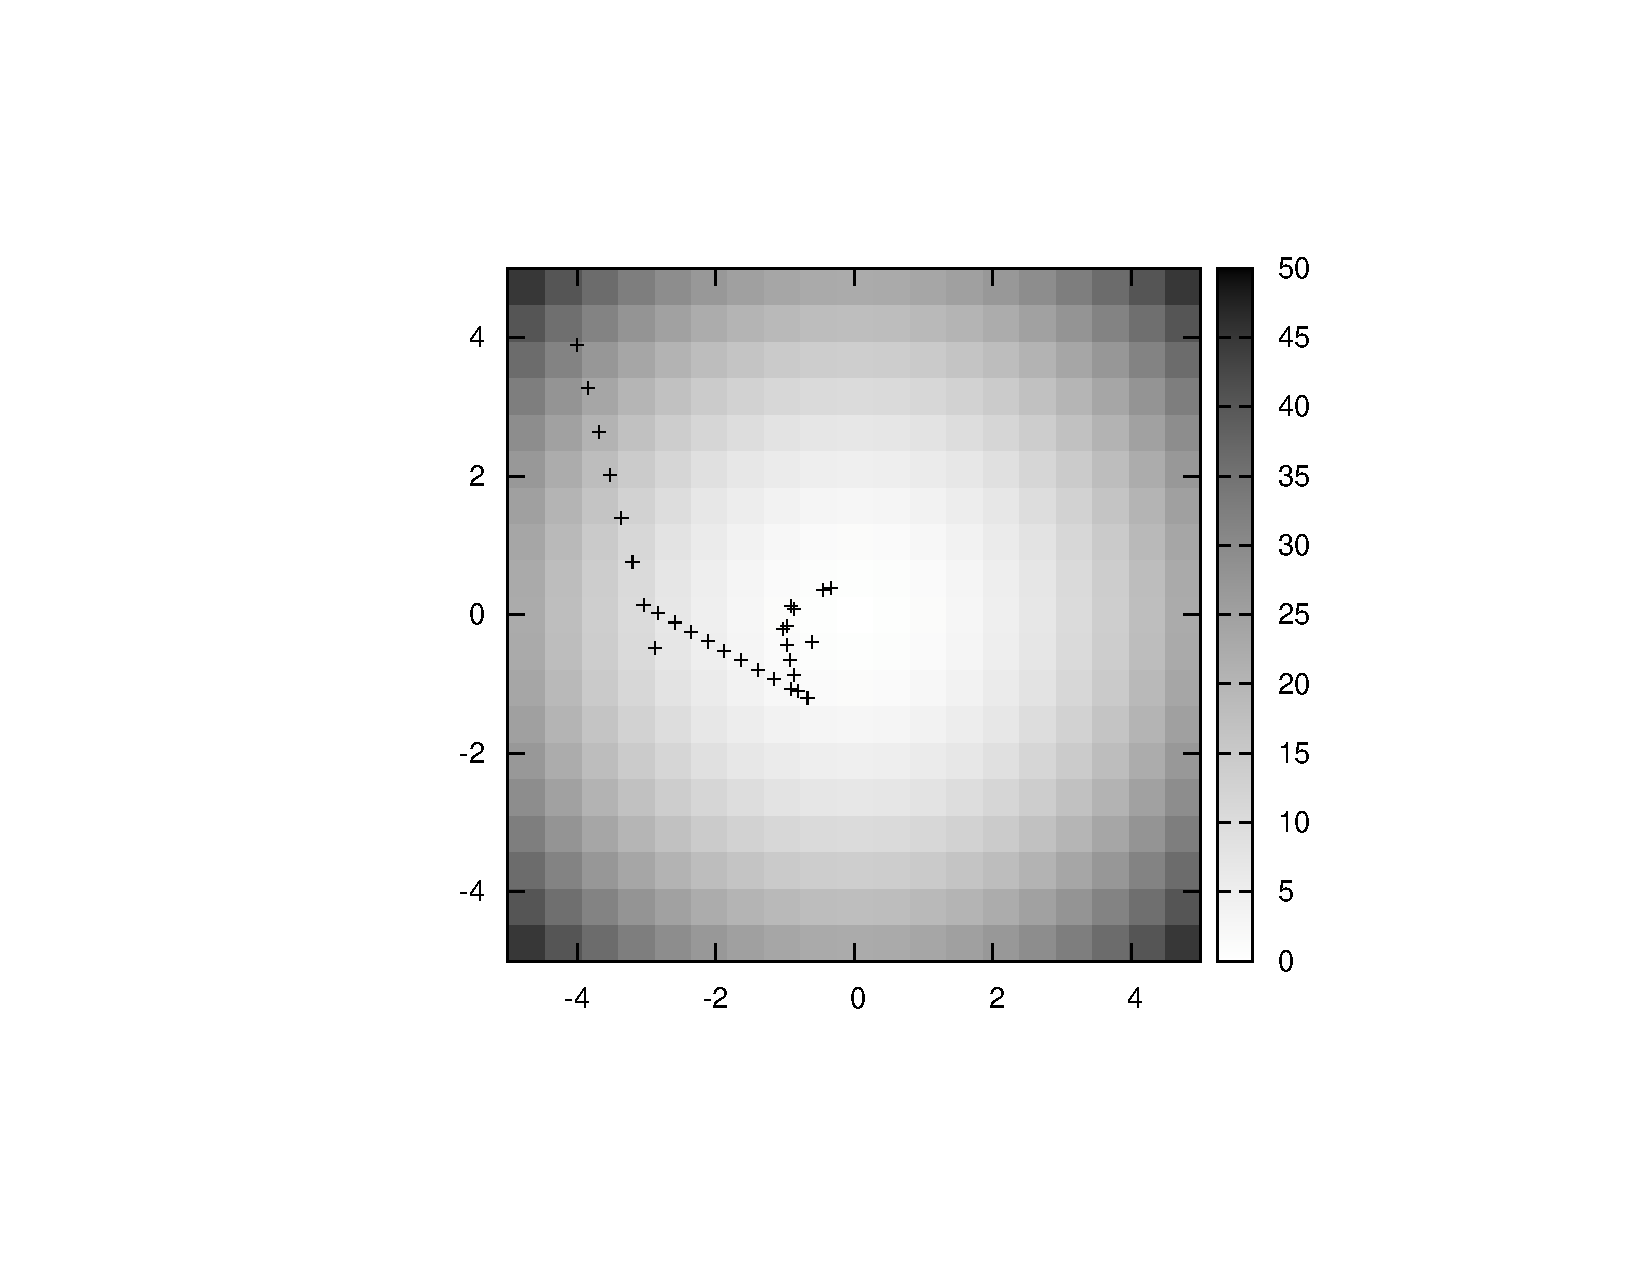
\includegraphics[trim = 2in 1.5in 2in 1.5in, clip, scale=0.5]{graphics/pso1.pdf}
\caption{Contour plot of the basin function showing the position of selected samples in the domain.}
\label{plot:pso1}
\end{figure}

Listing~\ref{pso1} provides the Gnuplot script used to prepare the plot, where \texttt{pso1.txt} is a file that contains the coordinates of the best solution found by the algorithm, with one coordinate per line separated by a space.

\begin{lstlisting}[caption=Gnuplot script use to create a contour plot and the position of selected samples from the domain., label=pso1]
set xrange [-5:5]
set yrange [-5:5]
set pm3d map
set palette gray negative
set samples 20
set isosamples 20
splot x*x+y*y, "pso1.txt" using 1:2:(0) with points
\end{lstlisting}

Listing~\ref{pso.file} provides a snippet of the first five lines of the \texttt{pso1.txt} file.

\begin{lstlisting}[caption=Snippet of the pso1.txt file., label=pso.file]
-3.9986483808224222 3.8910758979126956 31.12966051677087
-3.838580364459159 3.266132168962991 25.402318559546302
-3.678512348095896 2.6411884400132863 20.507329470753803
-3.518444331732633 2.0162447110635817 16.44469325039336
-3.35837631536937 1.391300982113877 13.214409898464986
...
\end{lstlisting}

% Traveling Salesman Problem
\subsubsection{Traveling Salesman Problem}
% general
Visualizing the results of a combinatorial optimization can provide insight into the areas of the problem that a selected technique is handling well, or  poorly.
Candidate solutions can be visualized over the course of a run to observe how the complexity of solutions found by a technique change over time. Alternatively, the best candidate solutions can be visualized at the end of a run. 

Candidate solutions for the Traveling Salesman Problem are easily visualized as tours (order of city visits) in the context of the city coordinates of the problem definition.

Figure~\ref{plot:tsp3} provides a plot of an example Nearest-Neighbor solution for the Berlin52 Traveling Salesman problem. A Nearest-Neighbor solution is constructed by randomly selecting the first city in the tour then selecting the next city in the tour with the minimum distance to the current city until a complete tour is created. 

\begin{figure}[htp]
\centering
% GNUPLOT: LaTeX picture
\setlength{\unitlength}{0.240900pt}
\ifx\plotpoint\undefined\newsavebox{\plotpoint}\fi
\sbox{\plotpoint}{\rule[-0.200pt]{0.400pt}{0.400pt}}%
\begin{picture}(1500,900)(0,0)
\sbox{\plotpoint}{\rule[-0.200pt]{0.400pt}{0.400pt}}%
\put(190.0,82.0){\rule[-0.200pt]{4.818pt}{0.400pt}}
\put(170,82){\makebox(0,0)[r]{ 0}}
\put(1430.0,82.0){\rule[-0.200pt]{4.818pt}{0.400pt}}
\put(190.0,212.0){\rule[-0.200pt]{4.818pt}{0.400pt}}
\put(170,212){\makebox(0,0)[r]{ 200}}
\put(1430.0,212.0){\rule[-0.200pt]{4.818pt}{0.400pt}}
\put(190.0,341.0){\rule[-0.200pt]{4.818pt}{0.400pt}}
\put(170,341){\makebox(0,0)[r]{ 400}}
\put(1430.0,341.0){\rule[-0.200pt]{4.818pt}{0.400pt}}
\put(190.0,471.0){\rule[-0.200pt]{4.818pt}{0.400pt}}
\put(170,471){\makebox(0,0)[r]{ 600}}
\put(1430.0,471.0){\rule[-0.200pt]{4.818pt}{0.400pt}}
\put(190.0,601.0){\rule[-0.200pt]{4.818pt}{0.400pt}}
\put(170,601){\makebox(0,0)[r]{ 800}}
\put(1430.0,601.0){\rule[-0.200pt]{4.818pt}{0.400pt}}
\put(190.0,730.0){\rule[-0.200pt]{4.818pt}{0.400pt}}
\put(170,730){\makebox(0,0)[r]{ 1000}}
\put(1430.0,730.0){\rule[-0.200pt]{4.818pt}{0.400pt}}
\put(190.0,860.0){\rule[-0.200pt]{4.818pt}{0.400pt}}
\put(170,860){\makebox(0,0)[r]{ 1200}}
\put(1430.0,860.0){\rule[-0.200pt]{4.818pt}{0.400pt}}
\put(190.0,82.0){\rule[-0.200pt]{0.400pt}{4.818pt}}
\put(190,41){\makebox(0,0){ 0}}
\put(190.0,840.0){\rule[-0.200pt]{0.400pt}{4.818pt}}
\put(330.0,82.0){\rule[-0.200pt]{0.400pt}{4.818pt}}
\put(330,41){\makebox(0,0){ 200}}
\put(330.0,840.0){\rule[-0.200pt]{0.400pt}{4.818pt}}
\put(470.0,82.0){\rule[-0.200pt]{0.400pt}{4.818pt}}
\put(470,41){\makebox(0,0){ 400}}
\put(470.0,840.0){\rule[-0.200pt]{0.400pt}{4.818pt}}
\put(610.0,82.0){\rule[-0.200pt]{0.400pt}{4.818pt}}
\put(610,41){\makebox(0,0){ 600}}
\put(610.0,840.0){\rule[-0.200pt]{0.400pt}{4.818pt}}
\put(750.0,82.0){\rule[-0.200pt]{0.400pt}{4.818pt}}
\put(750,41){\makebox(0,0){ 800}}
\put(750.0,840.0){\rule[-0.200pt]{0.400pt}{4.818pt}}
\put(890.0,82.0){\rule[-0.200pt]{0.400pt}{4.818pt}}
\put(890,41){\makebox(0,0){ 1000}}
\put(890.0,840.0){\rule[-0.200pt]{0.400pt}{4.818pt}}
\put(1030.0,82.0){\rule[-0.200pt]{0.400pt}{4.818pt}}
\put(1030,41){\makebox(0,0){ 1200}}
\put(1030.0,840.0){\rule[-0.200pt]{0.400pt}{4.818pt}}
\put(1170.0,82.0){\rule[-0.200pt]{0.400pt}{4.818pt}}
\put(1170,41){\makebox(0,0){ 1400}}
\put(1170.0,840.0){\rule[-0.200pt]{0.400pt}{4.818pt}}
\put(1310.0,82.0){\rule[-0.200pt]{0.400pt}{4.818pt}}
\put(1310,41){\makebox(0,0){ 1600}}
\put(1310.0,840.0){\rule[-0.200pt]{0.400pt}{4.818pt}}
\put(1450.0,82.0){\rule[-0.200pt]{0.400pt}{4.818pt}}
\put(1450,41){\makebox(0,0){ 1800}}
\put(1450.0,840.0){\rule[-0.200pt]{0.400pt}{4.818pt}}
\put(190.0,82.0){\rule[-0.200pt]{0.400pt}{187.420pt}}
\put(190.0,82.0){\rule[-0.200pt]{303.534pt}{0.400pt}}
\put(1450.0,82.0){\rule[-0.200pt]{0.400pt}{187.420pt}}
\put(190.0,860.0){\rule[-0.200pt]{303.534pt}{0.400pt}}
\put(1290,820){\makebox(0,0)[r]{"berlin52.nn.tour"}}
\put(1310.0,820.0){\rule[-0.200pt]{24.090pt}{0.400pt}}
\put(522,704){\usebox{\plotpoint}}
\multiput(522.00,704.58)(0.674,0.497){49}{\rule{0.638pt}{0.120pt}}
\multiput(522.00,703.17)(33.675,26.000){2}{\rule{0.319pt}{0.400pt}}
\multiput(555.92,716.14)(-0.491,-4.196){17}{\rule{0.118pt}{3.340pt}}
\multiput(556.17,723.07)(-10.000,-74.068){2}{\rule{0.400pt}{1.670pt}}
\multiput(547.58,646.50)(0.497,-0.629){59}{\rule{0.120pt}{0.603pt}}
\multiput(546.17,647.75)(31.000,-37.748){2}{\rule{0.400pt}{0.302pt}}
\multiput(578.58,598.08)(0.494,-3.545){25}{\rule{0.119pt}{2.871pt}}
\multiput(577.17,604.04)(14.000,-91.040){2}{\rule{0.400pt}{1.436pt}}
\multiput(592.58,510.53)(0.496,-0.619){39}{\rule{0.119pt}{0.595pt}}
\multiput(591.17,511.76)(21.000,-24.765){2}{\rule{0.400pt}{0.298pt}}
\multiput(611.92,484.69)(-0.497,-0.571){53}{\rule{0.120pt}{0.557pt}}
\multiput(612.17,485.84)(-28.000,-30.844){2}{\rule{0.400pt}{0.279pt}}
\multiput(576.01,455.59)(-2.751,0.482){9}{\rule{2.167pt}{0.116pt}}
\multiput(580.50,454.17)(-26.503,6.000){2}{\rule{1.083pt}{0.400pt}}
\multiput(547.47,459.92)(-1.867,-0.495){35}{\rule{1.574pt}{0.119pt}}
\multiput(550.73,460.17)(-66.734,-19.000){2}{\rule{0.787pt}{0.400pt}}
\multiput(482.94,442.00)(-0.468,7.500){5}{\rule{0.113pt}{5.300pt}}
\multiput(483.17,442.00)(-4.000,41.000){2}{\rule{0.400pt}{2.650pt}}
\multiput(478.92,494.00)(-0.498,0.756){95}{\rule{0.120pt}{0.704pt}}
\multiput(479.17,494.00)(-49.000,72.539){2}{\rule{0.400pt}{0.352pt}}
\multiput(426.36,566.92)(-1.277,-0.499){107}{\rule{1.118pt}{0.120pt}}
\multiput(428.68,567.17)(-137.679,-55.000){2}{\rule{0.559pt}{0.400pt}}
\multiput(291.58,510.60)(0.499,-0.596){215}{\rule{0.120pt}{0.577pt}}
\multiput(290.17,511.80)(109.000,-128.802){2}{\rule{0.400pt}{0.289pt}}
\multiput(400.00,381.92)(1.984,-0.497){61}{\rule{1.675pt}{0.120pt}}
\multiput(400.00,382.17)(122.523,-32.000){2}{\rule{0.838pt}{0.400pt}}
\multiput(526.00,349.92)(0.878,-0.497){61}{\rule{0.800pt}{0.120pt}}
\multiput(526.00,350.17)(54.340,-32.000){2}{\rule{0.400pt}{0.400pt}}
\multiput(582.00,317.94)(3.406,-0.468){5}{\rule{2.500pt}{0.113pt}}
\multiput(582.00,318.17)(18.811,-4.000){2}{\rule{1.250pt}{0.400pt}}
\multiput(606.00,315.59)(6.900,0.485){11}{\rule{5.300pt}{0.117pt}}
\multiput(606.00,314.17)(80.000,7.000){2}{\rule{2.650pt}{0.400pt}}
\multiput(695.92,322.00)(-0.495,2.513){31}{\rule{0.119pt}{2.076pt}}
\multiput(696.17,322.00)(-17.000,79.690){2}{\rule{0.400pt}{1.038pt}}
\multiput(677.76,458.58)(-0.547,0.491){17}{\rule{0.540pt}{0.118pt}}
\multiput(678.88,457.17)(-9.879,10.000){2}{\rule{0.270pt}{0.400pt}}
\put(680.0,406.0){\rule[-0.200pt]{0.400pt}{12.527pt}}
\multiput(669.00,477.58)(0.738,0.495){31}{\rule{0.688pt}{0.119pt}}
\multiput(669.00,476.17)(23.572,17.000){2}{\rule{0.344pt}{0.400pt}}
\multiput(694.00,494.59)(1.601,0.489){15}{\rule{1.344pt}{0.118pt}}
\multiput(694.00,493.17)(25.210,9.000){2}{\rule{0.672pt}{0.400pt}}
\multiput(722.00,501.95)(5.151,-0.447){3}{\rule{3.300pt}{0.108pt}}
\multiput(722.00,502.17)(17.151,-3.000){2}{\rule{1.650pt}{0.400pt}}
\multiput(744.92,497.34)(-0.495,-0.678){31}{\rule{0.119pt}{0.641pt}}
\multiput(745.17,498.67)(-17.000,-21.669){2}{\rule{0.400pt}{0.321pt}}
\put(669.0,468.0){\rule[-0.200pt]{0.400pt}{2.168pt}}
\multiput(771.61,477.00)(0.447,2.025){3}{\rule{0.108pt}{1.433pt}}
\multiput(770.17,477.00)(3.000,7.025){2}{\rule{0.400pt}{0.717pt}}
\multiput(774.59,487.00)(0.485,1.484){11}{\rule{0.117pt}{1.243pt}}
\multiput(773.17,487.00)(7.000,17.420){2}{\rule{0.400pt}{0.621pt}}
\put(729.0,477.0){\rule[-0.200pt]{10.118pt}{0.400pt}}
\multiput(781.00,521.92)(0.972,-0.493){23}{\rule{0.869pt}{0.119pt}}
\multiput(781.00,522.17)(23.196,-13.000){2}{\rule{0.435pt}{0.400pt}}
\multiput(806.00,510.58)(1.426,0.494){29}{\rule{1.225pt}{0.119pt}}
\multiput(806.00,509.17)(42.457,16.000){2}{\rule{0.613pt}{0.400pt}}
\multiput(851.58,520.21)(0.496,-1.637){39}{\rule{0.119pt}{1.395pt}}
\multiput(850.17,523.10)(21.000,-65.104){2}{\rule{0.400pt}{0.698pt}}
\multiput(868.88,456.92)(-0.816,-0.499){121}{\rule{0.752pt}{0.120pt}}
\multiput(870.44,457.17)(-99.440,-62.000){2}{\rule{0.376pt}{0.400pt}}
\multiput(769.92,392.84)(-0.499,-0.828){235}{\rule{0.120pt}{0.762pt}}
\multiput(770.17,394.42)(-119.000,-195.418){2}{\rule{0.400pt}{0.381pt}}
\multiput(645.13,199.58)(-1.955,0.498){87}{\rule{1.656pt}{0.120pt}}
\multiput(648.56,198.17)(-171.564,45.000){2}{\rule{0.828pt}{0.400pt}}
\multiput(424.16,244.59)(-16.816,0.485){11}{\rule{12.729pt}{0.117pt}}
\multiput(450.58,243.17)(-194.581,7.000){2}{\rule{6.364pt}{0.400pt}}
\multiput(251.52,249.92)(-1.237,-0.496){37}{\rule{1.080pt}{0.119pt}}
\multiput(253.76,250.17)(-46.758,-20.000){2}{\rule{0.540pt}{0.400pt}}
\put(781.0,507.0){\rule[-0.200pt]{0.400pt}{3.854pt}}
\multiput(207.00,202.58)(0.625,0.500){949}{\rule{0.600pt}{0.120pt}}
\multiput(207.00,201.17)(593.755,476.000){2}{\rule{0.300pt}{0.400pt}}
\multiput(799.68,678.58)(-0.573,0.499){271}{\rule{0.558pt}{0.120pt}}
\multiput(800.84,677.17)(-155.841,137.000){2}{\rule{0.279pt}{0.400pt}}
\multiput(641.78,815.58)(-0.848,0.497){55}{\rule{0.776pt}{0.120pt}}
\multiput(643.39,814.17)(-47.390,29.000){2}{\rule{0.388pt}{0.400pt}}
\multiput(596.00,842.92)(20.771,-0.491){17}{\rule{16.060pt}{0.118pt}}
\multiput(596.00,843.17)(365.667,-10.000){2}{\rule{8.030pt}{0.400pt}}
\multiput(995.58,830.06)(0.499,-1.061){263}{\rule{0.120pt}{0.948pt}}
\multiput(994.17,832.03)(133.000,-280.032){2}{\rule{0.400pt}{0.474pt}}
\multiput(1126.92,549.73)(-0.499,-0.559){165}{\rule{0.120pt}{0.548pt}}
\multiput(1127.17,550.86)(-84.000,-92.863){2}{\rule{0.400pt}{0.274pt}}
\multiput(1044.58,448.33)(0.496,-2.825){39}{\rule{0.119pt}{2.329pt}}
\multiput(1043.17,453.17)(21.000,-112.167){2}{\rule{0.400pt}{1.164pt}}
\multiput(1065.58,338.72)(0.498,-0.561){95}{\rule{0.120pt}{0.549pt}}
\multiput(1064.17,339.86)(49.000,-53.861){2}{\rule{0.400pt}{0.274pt}}
\multiput(1110.85,284.92)(-0.824,-0.498){87}{\rule{0.758pt}{0.120pt}}
\multiput(1112.43,285.17)(-72.427,-45.000){2}{\rule{0.379pt}{0.400pt}}
\multiput(1038.92,234.32)(-0.497,-1.902){59}{\rule{0.120pt}{1.610pt}}
\multiput(1039.17,237.66)(-31.000,-113.659){2}{\rule{0.400pt}{0.805pt}}
\multiput(1009.00,124.58)(1.173,0.499){173}{\rule{1.036pt}{0.120pt}}
\multiput(1009.00,123.17)(203.849,88.000){2}{\rule{0.518pt}{0.400pt}}
\multiput(1215.58,207.00)(0.498,-1.386){89}{\rule{0.120pt}{1.204pt}}
\multiput(1214.17,209.50)(46.000,-124.500){2}{\rule{0.400pt}{0.602pt}}
\multiput(1261.58,85.00)(0.499,0.530){291}{\rule{0.120pt}{0.524pt}}
\multiput(1260.17,85.00)(147.000,154.911){2}{\rule{0.400pt}{0.262pt}}
\multiput(1406.92,241.00)(-0.499,1.281){187}{\rule{0.120pt}{1.123pt}}
\multiput(1407.17,241.00)(-95.000,240.669){2}{\rule{0.400pt}{0.562pt}}
\multiput(1306.61,484.58)(-1.800,0.500){437}{\rule{1.538pt}{0.120pt}}
\multiput(1309.81,483.17)(-787.807,220.000){2}{\rule{0.769pt}{0.400pt}}
\put(522,704){\raisebox{-.8pt}{\makebox(0,0){$\Diamond$}}}
\put(557,730){\raisebox{-.8pt}{\makebox(0,0){$\Diamond$}}}
\put(547,649){\raisebox{-.8pt}{\makebox(0,0){$\Diamond$}}}
\put(578,610){\raisebox{-.8pt}{\makebox(0,0){$\Diamond$}}}
\put(592,513){\raisebox{-.8pt}{\makebox(0,0){$\Diamond$}}}
\put(613,487){\raisebox{-.8pt}{\makebox(0,0){$\Diamond$}}}
\put(585,455){\raisebox{-.8pt}{\makebox(0,0){$\Diamond$}}}
\put(554,461){\raisebox{-.8pt}{\makebox(0,0){$\Diamond$}}}
\put(484,442){\raisebox{-.8pt}{\makebox(0,0){$\Diamond$}}}
\put(480,494){\raisebox{-.8pt}{\makebox(0,0){$\Diamond$}}}
\put(431,568){\raisebox{-.8pt}{\makebox(0,0){$\Diamond$}}}
\put(291,513){\raisebox{-.8pt}{\makebox(0,0){$\Diamond$}}}
\put(400,383){\raisebox{-.8pt}{\makebox(0,0){$\Diamond$}}}
\put(526,351){\raisebox{-.8pt}{\makebox(0,0){$\Diamond$}}}
\put(582,319){\raisebox{-.8pt}{\makebox(0,0){$\Diamond$}}}
\put(606,315){\raisebox{-.8pt}{\makebox(0,0){$\Diamond$}}}
\put(697,322){\raisebox{-.8pt}{\makebox(0,0){$\Diamond$}}}
\put(680,406){\raisebox{-.8pt}{\makebox(0,0){$\Diamond$}}}
\put(680,458){\raisebox{-.8pt}{\makebox(0,0){$\Diamond$}}}
\put(669,468){\raisebox{-.8pt}{\makebox(0,0){$\Diamond$}}}
\put(669,477){\raisebox{-.8pt}{\makebox(0,0){$\Diamond$}}}
\put(694,494){\raisebox{-.8pt}{\makebox(0,0){$\Diamond$}}}
\put(722,503){\raisebox{-.8pt}{\makebox(0,0){$\Diamond$}}}
\put(746,500){\raisebox{-.8pt}{\makebox(0,0){$\Diamond$}}}
\put(729,477){\raisebox{-.8pt}{\makebox(0,0){$\Diamond$}}}
\put(771,477){\raisebox{-.8pt}{\makebox(0,0){$\Diamond$}}}
\put(774,487){\raisebox{-.8pt}{\makebox(0,0){$\Diamond$}}}
\put(781,507){\raisebox{-.8pt}{\makebox(0,0){$\Diamond$}}}
\put(781,523){\raisebox{-.8pt}{\makebox(0,0){$\Diamond$}}}
\put(806,510){\raisebox{-.8pt}{\makebox(0,0){$\Diamond$}}}
\put(851,526){\raisebox{-.8pt}{\makebox(0,0){$\Diamond$}}}
\put(872,458){\raisebox{-.8pt}{\makebox(0,0){$\Diamond$}}}
\put(771,396){\raisebox{-.8pt}{\makebox(0,0){$\Diamond$}}}
\put(652,199){\raisebox{-.8pt}{\makebox(0,0){$\Diamond$}}}
\put(477,244){\raisebox{-.8pt}{\makebox(0,0){$\Diamond$}}}
\put(256,251){\raisebox{-.8pt}{\makebox(0,0){$\Diamond$}}}
\put(207,231){\raisebox{-.8pt}{\makebox(0,0){$\Diamond$}}}
\put(207,202){\raisebox{-.8pt}{\makebox(0,0){$\Diamond$}}}
\put(802,678){\raisebox{-.8pt}{\makebox(0,0){$\Diamond$}}}
\put(645,815){\raisebox{-.8pt}{\makebox(0,0){$\Diamond$}}}
\put(596,844){\raisebox{-.8pt}{\makebox(0,0){$\Diamond$}}}
\put(995,834){\raisebox{-.8pt}{\makebox(0,0){$\Diamond$}}}
\put(1128,552){\raisebox{-.8pt}{\makebox(0,0){$\Diamond$}}}
\put(1044,458){\raisebox{-.8pt}{\makebox(0,0){$\Diamond$}}}
\put(1065,341){\raisebox{-.8pt}{\makebox(0,0){$\Diamond$}}}
\put(1114,286){\raisebox{-.8pt}{\makebox(0,0){$\Diamond$}}}
\put(1040,241){\raisebox{-.8pt}{\makebox(0,0){$\Diamond$}}}
\put(1009,124){\raisebox{-.8pt}{\makebox(0,0){$\Diamond$}}}
\put(1215,212){\raisebox{-.8pt}{\makebox(0,0){$\Diamond$}}}
\put(1261,85){\raisebox{-.8pt}{\makebox(0,0){$\Diamond$}}}
\put(1408,241){\raisebox{-.8pt}{\makebox(0,0){$\Diamond$}}}
\put(1313,484){\raisebox{-.8pt}{\makebox(0,0){$\Diamond$}}}
\put(522,704){\raisebox{-.8pt}{\makebox(0,0){$\Diamond$}}}
\put(1360,820){\raisebox{-.8pt}{\makebox(0,0){$\Diamond$}}}
\put(207.0,202.0){\rule[-0.200pt]{0.400pt}{6.986pt}}
\put(190.0,82.0){\rule[-0.200pt]{0.400pt}{187.420pt}}
\put(190.0,82.0){\rule[-0.200pt]{303.534pt}{0.400pt}}
\put(1450.0,82.0){\rule[-0.200pt]{0.400pt}{187.420pt}}
\put(190.0,860.0){\rule[-0.200pt]{303.534pt}{0.400pt}}
\end{picture}

\caption{Plot of the cities of a Nearest-Neighbor tour for the Berlin52 Traveling Salesman Problem.}
\label{plot:tsp3}
\end{figure}

Listing~\ref{tsp3} provides the Gnuplot script used to prepare the plot, where \texttt{berlin52.nn.tour} is a file that contains a listing of the coordinates of all cities in order that the cities are visited with one city per line separated by white space. The first city in the tour is repeated as the last city in the tour to provide a closed polygon in the plot.

\begin{lstlisting}[caption=Gnuplot script for plotting a tour for a Traveling Salesman Problem., label=tsp3]
plot "berlin52.nn.tour" with linespoints
\end{lstlisting}

Listing~\ref{tsp3.file} provides a snippet of the first five lines of the \texttt{berlin52.nn.tour} file.

\begin{lstlisting}[caption=Snippet of the berlin52.nn.tour file., label=tsp3.file]
475 960
525 1000
510 875
555 815
575 665
...
\end{lstlisting}

Figure~\ref{plot:tsp2} provides a plot of the known optimal solution for the Berlin52 Traveling Salesman problem. 

\begin{figure}[htp]
\centering
% GNUPLOT: LaTeX picture
\setlength{\unitlength}{0.240900pt}
\ifx\plotpoint\undefined\newsavebox{\plotpoint}\fi
\sbox{\plotpoint}{\rule[-0.200pt]{0.400pt}{0.400pt}}%
\begin{picture}(1500,900)(0,0)
\sbox{\plotpoint}{\rule[-0.200pt]{0.400pt}{0.400pt}}%
\put(150.0,82.0){\rule[-0.200pt]{4.818pt}{0.400pt}}
\put(130,82){\makebox(0,0)[r]{ 0}}
\put(1419.0,82.0){\rule[-0.200pt]{4.818pt}{0.400pt}}
\put(150.0,212.0){\rule[-0.200pt]{4.818pt}{0.400pt}}
\put(130,212){\makebox(0,0)[r]{ 200}}
\put(1419.0,212.0){\rule[-0.200pt]{4.818pt}{0.400pt}}
\put(150.0,341.0){\rule[-0.200pt]{4.818pt}{0.400pt}}
\put(130,341){\makebox(0,0)[r]{ 400}}
\put(1419.0,341.0){\rule[-0.200pt]{4.818pt}{0.400pt}}
\put(150.0,471.0){\rule[-0.200pt]{4.818pt}{0.400pt}}
\put(130,471){\makebox(0,0)[r]{ 600}}
\put(1419.0,471.0){\rule[-0.200pt]{4.818pt}{0.400pt}}
\put(150.0,600.0){\rule[-0.200pt]{4.818pt}{0.400pt}}
\put(130,600){\makebox(0,0)[r]{ 800}}
\put(1419.0,600.0){\rule[-0.200pt]{4.818pt}{0.400pt}}
\put(150.0,730.0){\rule[-0.200pt]{4.818pt}{0.400pt}}
\put(130,730){\makebox(0,0)[r]{ 1000}}
\put(1419.0,730.0){\rule[-0.200pt]{4.818pt}{0.400pt}}
\put(150.0,859.0){\rule[-0.200pt]{4.818pt}{0.400pt}}
\put(130,859){\makebox(0,0)[r]{ 1200}}
\put(1419.0,859.0){\rule[-0.200pt]{4.818pt}{0.400pt}}
\put(150.0,82.0){\rule[-0.200pt]{0.400pt}{4.818pt}}
\put(150,41){\makebox(0,0){ 0}}
\put(150.0,839.0){\rule[-0.200pt]{0.400pt}{4.818pt}}
\put(293.0,82.0){\rule[-0.200pt]{0.400pt}{4.818pt}}
\put(293,41){\makebox(0,0){ 200}}
\put(293.0,839.0){\rule[-0.200pt]{0.400pt}{4.818pt}}
\put(436.0,82.0){\rule[-0.200pt]{0.400pt}{4.818pt}}
\put(436,41){\makebox(0,0){ 400}}
\put(436.0,839.0){\rule[-0.200pt]{0.400pt}{4.818pt}}
\put(580.0,82.0){\rule[-0.200pt]{0.400pt}{4.818pt}}
\put(580,41){\makebox(0,0){ 600}}
\put(580.0,839.0){\rule[-0.200pt]{0.400pt}{4.818pt}}
\put(723.0,82.0){\rule[-0.200pt]{0.400pt}{4.818pt}}
\put(723,41){\makebox(0,0){ 800}}
\put(723.0,839.0){\rule[-0.200pt]{0.400pt}{4.818pt}}
\put(866.0,82.0){\rule[-0.200pt]{0.400pt}{4.818pt}}
\put(866,41){\makebox(0,0){ 1000}}
\put(866.0,839.0){\rule[-0.200pt]{0.400pt}{4.818pt}}
\put(1009.0,82.0){\rule[-0.200pt]{0.400pt}{4.818pt}}
\put(1009,41){\makebox(0,0){ 1200}}
\put(1009.0,839.0){\rule[-0.200pt]{0.400pt}{4.818pt}}
\put(1153.0,82.0){\rule[-0.200pt]{0.400pt}{4.818pt}}
\put(1153,41){\makebox(0,0){ 1400}}
\put(1153.0,839.0){\rule[-0.200pt]{0.400pt}{4.818pt}}
\put(1296.0,82.0){\rule[-0.200pt]{0.400pt}{4.818pt}}
\put(1296,41){\makebox(0,0){ 1600}}
\put(1296.0,839.0){\rule[-0.200pt]{0.400pt}{4.818pt}}
\put(1439.0,82.0){\rule[-0.200pt]{0.400pt}{4.818pt}}
\put(1439,41){\makebox(0,0){ 1800}}
\put(1439.0,839.0){\rule[-0.200pt]{0.400pt}{4.818pt}}
\put(150.0,82.0){\rule[-0.200pt]{0.400pt}{187.179pt}}
\put(150.0,82.0){\rule[-0.200pt]{310.520pt}{0.400pt}}
\put(1439.0,82.0){\rule[-0.200pt]{0.400pt}{187.179pt}}
\put(150.0,859.0){\rule[-0.200pt]{310.520pt}{0.400pt}}
\put(1279,819){\makebox(0,0)[r]{"./berlin52.optimal"}}
\put(1299.0,819.0){\rule[-0.200pt]{24.090pt}{0.400pt}}
\put(555,454){\usebox{\plotpoint}}
\multiput(555.58,454.00)(0.497,0.589){53}{\rule{0.120pt}{0.571pt}}
\multiput(554.17,454.00)(28.000,31.814){2}{\rule{0.400pt}{0.286pt}}
\multiput(581.92,487.00)(-0.496,0.619){39}{\rule{0.119pt}{0.595pt}}
\multiput(582.17,487.00)(-21.000,24.765){2}{\rule{0.400pt}{0.298pt}}
\multiput(560.92,513.00)(-0.494,3.302){27}{\rule{0.119pt}{2.687pt}}
\multiput(561.17,513.00)(-15.000,91.424){2}{\rule{0.400pt}{1.343pt}}
\multiput(545.92,610.00)(-0.497,0.609){61}{\rule{0.120pt}{0.588pt}}
\multiput(546.17,610.00)(-32.000,37.781){2}{\rule{0.400pt}{0.294pt}}
\multiput(513.92,649.00)(-0.497,1.107){47}{\rule{0.120pt}{0.980pt}}
\multiput(514.17,649.00)(-25.000,52.966){2}{\rule{0.400pt}{0.490pt}}
\multiput(490.00,704.58)(0.693,0.497){49}{\rule{0.654pt}{0.120pt}}
\multiput(490.00,703.17)(34.643,26.000){2}{\rule{0.327pt}{0.400pt}}
\multiput(526.58,730.00)(0.498,1.456){75}{\rule{0.120pt}{1.259pt}}
\multiput(525.17,730.00)(39.000,110.387){2}{\rule{0.400pt}{0.629pt}}
\multiput(565.00,841.92)(0.865,-0.497){55}{\rule{0.790pt}{0.120pt}}
\multiput(565.00,842.17)(48.361,-29.000){2}{\rule{0.395pt}{0.400pt}}
\multiput(615.00,812.92)(0.596,-0.499){269}{\rule{0.576pt}{0.120pt}}
\multiput(615.00,813.17)(160.804,-136.000){2}{\rule{0.288pt}{0.400pt}}
\multiput(777.00,678.58)(0.636,0.499){307}{\rule{0.608pt}{0.120pt}}
\multiput(777.00,677.17)(195.737,155.000){2}{\rule{0.304pt}{0.400pt}}
\multiput(974.58,829.14)(0.499,-1.038){269}{\rule{0.120pt}{0.929pt}}
\multiput(973.17,831.07)(136.000,-280.071){2}{\rule{0.400pt}{0.465pt}}
\multiput(1110.00,549.92)(1.394,-0.499){133}{\rule{1.212pt}{0.120pt}}
\multiput(1110.00,550.17)(186.485,-68.000){2}{\rule{0.606pt}{0.400pt}}
\multiput(1299.58,478.44)(0.499,-1.250){191}{\rule{0.120pt}{1.098pt}}
\multiput(1298.17,480.72)(97.000,-239.721){2}{\rule{0.400pt}{0.549pt}}
\multiput(1394.92,238.86)(-0.499,-0.520){297}{\rule{0.120pt}{0.516pt}}
\multiput(1395.17,239.93)(-150.000,-154.929){2}{\rule{0.400pt}{0.258pt}}
\multiput(1244.92,85.00)(-0.498,1.357){91}{\rule{0.120pt}{1.181pt}}
\multiput(1245.17,85.00)(-47.000,124.549){2}{\rule{0.400pt}{0.590pt}}
\multiput(1194.60,210.92)(-1.201,-0.499){173}{\rule{1.059pt}{0.120pt}}
\multiput(1196.80,211.17)(-208.802,-88.000){2}{\rule{0.530pt}{0.400pt}}
\multiput(988.58,124.00)(0.497,1.842){61}{\rule{0.120pt}{1.562pt}}
\multiput(987.17,124.00)(32.000,113.757){2}{\rule{0.400pt}{0.781pt}}
\multiput(1020.00,241.58)(0.835,0.498){87}{\rule{0.767pt}{0.120pt}}
\multiput(1020.00,240.17)(73.409,45.000){2}{\rule{0.383pt}{0.400pt}}
\multiput(1093.92,286.00)(-0.498,0.550){97}{\rule{0.120pt}{0.540pt}}
\multiput(1094.17,286.00)(-50.000,53.879){2}{\rule{0.400pt}{0.270pt}}
\multiput(1043.92,341.00)(-0.496,2.825){39}{\rule{0.119pt}{2.329pt}}
\multiput(1044.17,341.00)(-21.000,112.167){2}{\rule{0.400pt}{1.164pt}}
\multiput(846.92,458.00)(-0.496,1.637){39}{\rule{0.119pt}{1.395pt}}
\multiput(847.17,458.00)(-21.000,65.104){2}{\rule{0.400pt}{0.698pt}}
\multiput(821.99,524.92)(-1.400,-0.495){31}{\rule{1.206pt}{0.119pt}}
\multiput(824.50,525.17)(-44.497,-17.000){2}{\rule{0.603pt}{0.400pt}}
\multiput(776.39,509.58)(-0.972,0.493){23}{\rule{0.869pt}{0.119pt}}
\multiput(778.20,508.17)(-23.196,13.000){2}{\rule{0.435pt}{0.400pt}}
\put(848.0,458.0){\rule[-0.200pt]{42.398pt}{0.400pt}}
\multiput(753.93,501.08)(-0.485,-1.408){11}{\rule{0.117pt}{1.186pt}}
\multiput(754.17,503.54)(-7.000,-16.539){2}{\rule{0.400pt}{0.593pt}}
\multiput(746.94,482.43)(-0.468,-1.358){5}{\rule{0.113pt}{1.100pt}}
\multiput(747.17,484.72)(-4.000,-7.717){2}{\rule{0.400pt}{0.550pt}}
\multiput(741.78,477.58)(-0.542,0.496){43}{\rule{0.535pt}{0.120pt}}
\multiput(742.89,476.17)(-23.890,23.000){2}{\rule{0.267pt}{0.400pt}}
\multiput(717.92,497.46)(-0.495,-0.639){33}{\rule{0.119pt}{0.611pt}}
\multiput(718.17,498.73)(-18.000,-21.732){2}{\rule{0.400pt}{0.306pt}}
\multiput(699.93,477.00)(-0.485,1.942){11}{\rule{0.117pt}{1.586pt}}
\multiput(700.17,477.00)(-7.000,22.709){2}{\rule{0.400pt}{0.793pt}}
\multiput(688.94,501.92)(-1.433,-0.491){17}{\rule{1.220pt}{0.118pt}}
\multiput(691.47,502.17)(-25.468,-10.000){2}{\rule{0.610pt}{0.400pt}}
\multiput(662.99,491.92)(-0.785,-0.494){29}{\rule{0.725pt}{0.119pt}}
\multiput(664.50,492.17)(-23.495,-16.000){2}{\rule{0.363pt}{0.400pt}}
\put(755.0,506.0){\rule[-0.200pt]{0.400pt}{3.854pt}}
\multiput(641.00,465.93)(0.553,-0.489){15}{\rule{0.544pt}{0.118pt}}
\multiput(641.00,466.17)(8.870,-9.000){2}{\rule{0.272pt}{0.400pt}}
\put(641.0,467.0){\rule[-0.200pt]{0.400pt}{2.409pt}}
\multiput(651.00,404.92)(4.821,-0.491){17}{\rule{3.820pt}{0.118pt}}
\multiput(651.00,405.17)(85.071,-10.000){2}{\rule{1.910pt}{0.400pt}}
\multiput(741.90,394.92)(-0.506,-0.499){145}{\rule{0.505pt}{0.120pt}}
\multiput(742.95,395.17)(-73.951,-74.000){2}{\rule{0.253pt}{0.400pt}}
\multiput(667.92,317.15)(-0.498,-1.343){89}{\rule{0.120pt}{1.170pt}}
\multiput(668.17,319.57)(-46.000,-120.573){2}{\rule{0.400pt}{0.585pt}}
\multiput(621.92,199.00)(-0.498,1.239){91}{\rule{0.120pt}{1.087pt}}
\multiput(622.17,199.00)(-47.000,113.743){2}{\rule{0.400pt}{0.544pt}}
\multiput(561.75,315.61)(-5.374,0.447){3}{\rule{3.433pt}{0.108pt}}
\multiput(568.87,314.17)(-17.874,3.000){2}{\rule{1.717pt}{0.400pt}}
\multiput(547.72,318.58)(-0.866,0.497){63}{\rule{0.791pt}{0.120pt}}
\multiput(549.36,317.17)(-55.358,33.000){2}{\rule{0.395pt}{0.400pt}}
\multiput(492.92,347.03)(-0.498,-1.073){97}{\rule{0.120pt}{0.956pt}}
\multiput(493.17,349.02)(-50.000,-105.016){2}{\rule{0.400pt}{0.478pt}}
\multiput(432.67,242.92)(-3.308,-0.498){81}{\rule{2.729pt}{0.120pt}}
\multiput(438.34,243.17)(-270.337,-42.000){2}{\rule{1.364pt}{0.400pt}}
\put(651.0,406.0){\rule[-0.200pt]{0.400pt}{12.527pt}}
\multiput(168.00,231.58)(1.330,0.495){35}{\rule{1.153pt}{0.119pt}}
\multiput(168.00,230.17)(47.608,19.000){2}{\rule{0.576pt}{0.400pt}}
\multiput(218.00,250.58)(0.552,0.499){263}{\rule{0.542pt}{0.120pt}}
\multiput(218.00,249.17)(145.875,133.000){2}{\rule{0.271pt}{0.400pt}}
\multiput(363.92,383.00)(-0.499,0.586){219}{\rule{0.120pt}{0.568pt}}
\multiput(364.17,383.00)(-111.000,128.820){2}{\rule{0.400pt}{0.284pt}}
\multiput(254.00,513.58)(1.304,0.499){107}{\rule{1.140pt}{0.120pt}}
\multiput(254.00,512.17)(140.634,55.000){2}{\rule{0.570pt}{0.400pt}}
\multiput(397.58,565.09)(0.498,-0.751){97}{\rule{0.120pt}{0.700pt}}
\multiput(396.17,566.55)(50.000,-73.547){2}{\rule{0.400pt}{0.350pt}}
\multiput(447.60,471.00)(0.468,-7.500){5}{\rule{0.113pt}{5.300pt}}
\multiput(446.17,482.00)(4.000,-41.000){2}{\rule{0.400pt}{2.650pt}}
\multiput(451.00,441.58)(1.797,0.496){37}{\rule{1.520pt}{0.119pt}}
\multiput(451.00,440.17)(67.845,20.000){2}{\rule{0.760pt}{0.400pt}}
\multiput(522.00,459.93)(2.476,-0.485){11}{\rule{1.986pt}{0.117pt}}
\multiput(522.00,460.17)(28.879,-7.000){2}{\rule{0.993pt}{0.400pt}}
\put(555,454){\makebox(0,0){$+$}}
\put(583,487){\makebox(0,0){$+$}}
\put(562,513){\makebox(0,0){$+$}}
\put(547,610){\makebox(0,0){$+$}}
\put(515,649){\makebox(0,0){$+$}}
\put(490,704){\makebox(0,0){$+$}}
\put(526,730){\makebox(0,0){$+$}}
\put(565,843){\makebox(0,0){$+$}}
\put(615,814){\makebox(0,0){$+$}}
\put(777,678){\makebox(0,0){$+$}}
\put(974,833){\makebox(0,0){$+$}}
\put(1110,551){\makebox(0,0){$+$}}
\put(1299,483){\makebox(0,0){$+$}}
\put(1396,241){\makebox(0,0){$+$}}
\put(1246,85){\makebox(0,0){$+$}}
\put(1199,212){\makebox(0,0){$+$}}
\put(988,124){\makebox(0,0){$+$}}
\put(1020,241){\makebox(0,0){$+$}}
\put(1095,286){\makebox(0,0){$+$}}
\put(1045,341){\makebox(0,0){$+$}}
\put(1024,458){\makebox(0,0){$+$}}
\put(848,458){\makebox(0,0){$+$}}
\put(827,526){\makebox(0,0){$+$}}
\put(780,509){\makebox(0,0){$+$}}
\put(755,522){\makebox(0,0){$+$}}
\put(755,506){\makebox(0,0){$+$}}
\put(748,487){\makebox(0,0){$+$}}
\put(744,477){\makebox(0,0){$+$}}
\put(719,500){\makebox(0,0){$+$}}
\put(701,477){\makebox(0,0){$+$}}
\put(694,503){\makebox(0,0){$+$}}
\put(666,493){\makebox(0,0){$+$}}
\put(641,477){\makebox(0,0){$+$}}
\put(641,467){\makebox(0,0){$+$}}
\put(651,458){\makebox(0,0){$+$}}
\put(651,406){\makebox(0,0){$+$}}
\put(744,396){\makebox(0,0){$+$}}
\put(669,322){\makebox(0,0){$+$}}
\put(623,199){\makebox(0,0){$+$}}
\put(576,315){\makebox(0,0){$+$}}
\put(551,318){\makebox(0,0){$+$}}
\put(494,351){\makebox(0,0){$+$}}
\put(444,244){\makebox(0,0){$+$}}
\put(168,202){\makebox(0,0){$+$}}
\put(168,231){\makebox(0,0){$+$}}
\put(218,250){\makebox(0,0){$+$}}
\put(365,383){\makebox(0,0){$+$}}
\put(254,513){\makebox(0,0){$+$}}
\put(397,568){\makebox(0,0){$+$}}
\put(447,493){\makebox(0,0){$+$}}
\put(451,441){\makebox(0,0){$+$}}
\put(522,461){\makebox(0,0){$+$}}
\put(555,454){\makebox(0,0){$+$}}
\put(1349,819){\makebox(0,0){$+$}}
\put(168.0,202.0){\rule[-0.200pt]{0.400pt}{6.986pt}}
\put(150.0,82.0){\rule[-0.200pt]{0.400pt}{187.179pt}}
\put(150.0,82.0){\rule[-0.200pt]{310.520pt}{0.400pt}}
\put(1439.0,82.0){\rule[-0.200pt]{0.400pt}{187.179pt}}
\put(150.0,859.0){\rule[-0.200pt]{310.520pt}{0.400pt}}
\end{picture}

\caption{Plot of the cities of the optimal tour for the Berlin52 Traveling Salesman Problem.}
\label{plot:tsp2}
\end{figure}

Listing~\ref{tsp2} provides the Gnuplot script used to prepare the plot, where \texttt{berlin52.optimal} is a file that contains a listing of the coordinates of all cities in order that the cities are visited with one city per line separated by white space. The first city in the tour is repeated as the last city in the tour to provide a closed polygon in the plot.

\begin{lstlisting}[caption=Gnuplot script for plotting a tour for a Traveling Salesman Problem., label=tsp2]
plot "berlin52.optimal" with linespoints
\end{lstlisting}

Listing~\ref{tsp2.file} provides a snippet of the first five lines of the \texttt{berlin52.optimal} file.

\begin{lstlisting}[caption=Snippet of the berlin52.optimal file., label=tsp2.file]
565.0 575.0
605.0 625.0
575.0 665.0
555.0 815.0
510.0 875.0
...
\end{lstlisting}
